%% filename: amsbook-template.tex
%% version: 1.1
%% date: 2014/07/24
%%
%% American Mathematical Society
%% Technical Support
%% Publications Technical Group
%% 201 Charles Street
%% Providence, RI 02904
%% USA
%% tel: (401) 455-4080
%%      (800) 321-4267 (USA and Canada only)
%% fax: (401) 331-3842
%% email: tech-support@ams.org
%% 
%% Copyright 2006, 2008-2010, 2014 American Mathematical Society.
%% 
%% This work may be distributed and/or modified under the
%% conditions of the LaTeX Project Public License, either version 1.3c
%% of this license or (at your option) any later version.
%% The latest version of this license is in
%%   http://www.latex-project.org/lppl.txt
%% and version 1.3c or later is part of all distributions of LaTeX
%% version 2005/12/01 or later.
%% 
%% This work has the LPPL maintenance status `maintained'.
%% 
%% The Current Maintainer of this work is the American Mathematical
%% Society.
%%
%% ====================================================================

%    AMS-LaTeX v.2 driver file template for use with amsbook
%
%    Remove any commented or uncommented macros you do not use.

\documentclass[ebook, oneside, openany]{book}
\usepackage{amsfonts,bm,amsthm,amsmath,bbm,amssymb,mathtools}
\usepackage{fullpage}
\usepackage{tikz, pgfplots} % added for Lecture 2	
\usepackage{caption, subcaption}
\usepackage{float}  % added for Lecture 8
\usepackage[ruled,vlined,linesnumbered]{algorithm2e}  % added for Lecture 15
\usepackage{booktabs}  % added for Lecture 15
\usepackage{hyperref}
\hypersetup{linktocpage}
\usepackage{natbib}
\renewcommand{\cite}[1]{\citep{#1}}



\newtheorem{theorem}{Theorem}[chapter]
\newtheorem{lemma}[theorem]{Lemma}

\theoremstyle{definition}
\newtheorem{definition}[theorem]{Definition}
\newtheorem{example}[theorem]{Example}
\newtheorem{xca}[theorem]{Exercise}
\newtheorem{corollary}[theorem]{Corollary}  % added for Lecture 5
\newtheorem{proposition}{Proposition}[section]  % added for Lecture 6

\theoremstyle{remark}
\newtheorem{remark}[theorem]{Remark}

\numberwithin{section}{chapter}
\numberwithin{equation}{chapter}

%    For a single index; for multiple indexes, see the manual
%    "Instructions for preparation of papers and monographs:
%    AMS-LaTeX" (instr-l.pdf in the AMS-LaTeX distribution).
\makeindex
\def\lectureformat{0}
\usepackage{color}
\usepackage{lipsum}


% for potential improvements
\def\shownotes{0}  %set 1 to show author notes
\ifnum\shownotes=1
\newcommand{\authnoteimp}[2]{[#1: #2]}
\else
\newcommand{\authnoteimp}[2]{}
\fi
\newcommand{\tnoteimp}[1]{{\color{blue}\authnoteimp{todo}{#1}}}
\newcommand{\tnote}[1]{{\color{blue}\authnoteimp{TM}{#1}}}
\newcommand{\todo}[1]{\tnoteimp{#1}}


% for course staff to edit or comment
\def\shownotes{0}  %set 1 to show author notes
\ifnum\shownotes=1
\newcommand{\authnote}[2]{[#1: #2]}
\else
\newcommand{\authnote}[2]{}
\fi
\newcommand{\ttodo}[1]{{\color{blue}\authnote{todo for TM}{#1}}}


% for long term commnets 
\def\shownotes{0}  %set 1 to show author notes
\ifnum\shownotes=1
\newcommand{\authnotelong}[2]{[#1: #2]}
\else
\newcommand{\authnotelong}[2]{}
\fi
\newcommand{\tnotelong}[1]{{\color{blue}\authnotelong{TM}{#1}}}




\ifnum\lectureformat=1
\newcommand{\metadata}[3]
{
	\newpage
	
	\def\lectureID{#1}
	
	\setcounter{chapter}{\lectureID}

%	\draftnotice
	
	\begin{center}
		\bf\large CS229M/STATS214: Machine Learning Theory
	\end{center}
	
	\noindent
	Lecturer: Tengyu Ma   %%% FILL IN LECTURER (if not RS)
	\hfill
	Lecture \# \lectureID              %%% FILL IN LECTURE NUMBER HERE
	\\
	Scribe: #2                  %%% FILL IN YOUR NAME HERE
	\hfill
	#3           %%% FILL IN LECTURE DATE HERE
	
	\noindent
	\rule{\textwidth}{1pt}
	
	\medskip
}
\else 
\newcommand{\metadata}[3]{}
\fi

\newcommand*\circled[1]{\tikz[baseline=(char.base)]{
	\node[shape=circle,draw,inner sep=2pt] (char) {#1};}}

\DeclareMathOperator*{\Exp}{\mathbb{E}}
\DeclareMathOperator*{\argmin}{\textup{argmin}}
\DeclareMathOperator*{\argmax}{\textup{argmax}}

\newcommand{\Cov}{\operatorname{Cov}}
\newcommand{\KL}{\operatorname{KL}}
\newcommand{\margin}{\text{margin}}
\newcommand{\poly}{\operatorname{poly}}
\newcommand{\sd}{\operatorname{sd}}
\newcommand{\sgn}{\text{sgn}}
\newcommand{\tr}{\operatorname{tr}}
\newcommand{\Var}{\operatorname{Var}}
\newcommand{\ind}[1]{\mathbf{1}[#1]}

\newcommand{\err}{\ell_{\textup{0-1}}}
\newcommand{\Err}{L_{\textup{0-1}}}
\newcommand{\thetaerm}{\theta_{\textup{ERM}}}
\newcommand{\hatL}{\widehat{L}}
\newcommand{\tilO}{\widetilde{O}}
\newcommand{\iid}{\overset{\textup{iid}}{\sim}}
\newcommand\defeq{\stackrel{\mathclap{\tiny \mbox{$\Delta$}}}{=}}

\newcommand{\gammamin}{\gamma_{\mathrm{min}}}
\newcommand{\phirelu}{\phi_{\textup{relu}}}
\newcommand{\supunitball}{\sup_{\overline{u}:\norm{\overline{u}}_2 \le 1}}
\newcommand{\ubar}{\overline{u}}
\renewcommand{\Phi}{\varphi}
\newcommand{\thetazero}{\theta^{0}}
\newcommand{\popL}{L(\beta)}
\newcommand{\empL}{\hatL(\beta)}
\newcommand{\popLt}{L(\beta^t)}
\newcommand{\empLt}{\hatL(\beta^t)}
\newcommand{\yhat}[0]{\hat{y}}

\newcommand{\norm}[1]{\|#1\|}
\newcommand{\Norm}[1]{\left\|#1\right\|}
\renewcommand{\l}{\left}
\renewcommand{\r}{\right}
\newcommand{\rbr}[1]{\left(#1\right)}
\newcommand{\sbr}[1]{\left[#1\right]}
\newcommand{\cbr}[1]{\left\{#1\right\}}
\newcommand{\abs}[1]{\left\lvert#1\right\rvert}
\newcommand{\inprod}[1]{\left\langle#1\right\rangle}
\renewcommand{\because}{{\textup{because}~}}

\newcommand{\al}[1]{
	\begin{align}
	#1
	\end{align}
}

\renewcommand{\sp}[1]{^{(#1)}}

\newcommand{\cA}{\mathcal A}	
\newcommand{\cB}{\mathcal B}
\newcommand{\cC}{\mathcal C}
\newcommand{\cD}{\mathcal D}
\newcommand{\cE}{\mathcal E}
\newcommand{\cF}{\mathcal F}
\newcommand{\cG}{\mathcal G}
\newcommand{\cH}{\mathcal H}
\newcommand{\cI}{\mathcal I}
\newcommand{\cJ}{\mathcal J}
\newcommand{\cK}{\mathcal K}
\newcommand{\cL}{\mathcal L}
\newcommand{\cM}{\mathcal M}
\newcommand{\cN}{\mathcal N}
\newcommand{\cO}{\mathcal O}
\newcommand{\cP}{\mathcal P}
\newcommand{\cQ}{\mathcal Q}
\newcommand{\cR}{\mathcal R}
\newcommand{\cS}{\mathcal S}
\newcommand{\cT}{\mathcal T}
\newcommand{\cU}{\mathcal U}
\newcommand{\cV}{\mathcal V}
\newcommand{\cW}{\mathcal W}
\newcommand{\cX}{\mathcal X}
\newcommand{\cY}{\mathcal Y}
\newcommand{\cZ}{\mathcal Z}

\newcommand{\bbB}{\mathbb B}
\newcommand{\bbS}{\mathbb S}
\newcommand{\bbR}{\mathbb R}
\newcommand{\bbZ}{\mathbb Z}
\newcommand{\bbI}{\mathbb I}
\newcommand{\bbQ}{\mathbb Q}
\newcommand{\bbP}{\mathbb P}
\newcommand{\bbE}{\mathbb E}
\newcommand{\bbN}{\mathbb N}

\newcommand{\N}{\mathbb{N}}
\newcommand{\R}{\bbR}
\newcommand{\Z}{\mathbb{Z}}



\begin{document}
	
	\frontmatter
	
	\title{Lecture Notes for Machine Learning Theory (CS229M/STATS214)}
	
	%    Remove any unused author tags.
	
	%    author one information
	\author{Instructor: Tengyu Ma
	}
	%\address{}
	%\curraddr{}
	%\email{}
	%\thanks{}
	
	%    author two information
	%\author{}
	%\address{}
	%\curraddr{}
	%\email{}
	%\thanks{}
	
	%\subjclass[2010]{Primary }
	
	%\keywords{}
	
	%\date{}
	
	%\begin{abstract}
	%\end{abstract}
	
	
	\maketitle
	
	%    Dedication.  If the dedication is longer than a line or two,
	%    remove the centering instructions and the line break.
	%\cleardoublepage
	%\thispagestyle{empty}
	%\vspace*{13.5pc}
	%\begin{center}
	%  Dedication text (use \\[2pt] for line break if necessary)
	%\end{center}
	%\cleardoublepage
	
	%    Change page number to 6 if a dedication is present.
	%\setcounter{page}{1}
	
	\tableofcontents
	
	%    Include unnumbered chapters (preface, acknowledgments, etc.) here.
	%\include{}
	\mainmatter
	\let\sec\section
	\let\subsec\subsection
	
	\chapter*{Acknowledgments}
	\setcounter{page}{5}
	This monograph is a collection of scribe notes for the course CS229M/STATS214 at Stanford University. The materials in Chapter \ref{chap:supervised}--\ref{chap:gen-bounds} are mostly based on Percy Liang's lecture notes~\cite{percynotes}, and Chapter~\ref{chap:OL} is largely based on Haipeng Luo's lectures~\cite{haipengnotes}. Kenneth Tay contributed significantly to the revision of these notes as a teaching assistant for the course. The original contributor to the scribe notes are Stanford students including but not limited to Anusri Pampari, Gabriel Poesia, Alexander Ke, Trenton Chang, Brad Ross, Robbie Jones, Yizhou Qian, Will Song, Daniel Do, Spencer M. Richards, Thomas Lew, David Lin, Jinhui Wang, Rafael Rafailov, Aidan Perreault,Kevin Han, Han Wu, Andrew Wang, Rohan Taori, Jonathan Lee, Rohith Kuditipudi, Kefan Dong, Roshni Sahoo, Sarah Wu, Tianyu Du, Xin Lu, Soham Sinha, Kevin Guo, Jeff Z. HaoChen, Carrie Wu, Kaidi Cao, and Ruocheng Wang.  The notes will be updated every year with new materials. The reference list is far from complete. 
	
	
	\chapter{Supervised Learning Formulations}\label{chap:supervised}
	% reset section counter

\setcounter{section}{0}

\metadata{1}{Anusri Pampari and Gabriel Poesia}{Jan 11th, 2021}


In this chapter, we will set up the standard theoretical formulation of supervised learning and introduce the \textit{empirical risk minimization} (ERM) paradigm. The setup will apply to almost the entire monograph \tnotelong{to be updated}and the ERM paradigm will be the main focus of Chapter~\ref{chap:asymp}, \ref{chap:conc}, and \ref{chap:uc}. 

\sec{Supervised learning}\label{lec1:sec:sup-learn}
In supervised learning, we have a dataset where each data point is associated with a label, and we aim to learn from the data a function that maps data points to their labels. The learned  function can be used to infer the labels of test data points. More formally, suppose the data points, also called inputs,  belong to some input space $\cX$ (e.g. images of birds), and labels belong to the output space $\cY$ (e.g. bird species). Suppose we are interested in a specific joint probability distribution $P$ over $\cX \times \cY$ (e.g. images of birds in North America), from which we draw a \emph{training set}, i.e we draw a a set of $n$ independent and identically distributed (i.i.d.) data points $\{(x^{(i)}, y^{(i)}\}_{i=1}^n$ from $P$. The goal of supervised learning is to learn a mapping (i.e. a function) from $\cX$ to $\cY$ using the training data. Any such function $h : \cX \rightarrow \cY$ is called a \emph{predictor} (also \emph{hypothesis} or \emph{model}).

Given two predictors, how do we decide which is better? For that, we define a \emph{loss function} over the predictions. There are several ways to define loss functions: for now, define a loss function $\ell$ as a function $\ell : \cY \times \cY \rightarrow \R$. Intuitively, the loss function takes two labels, the prediction made by a model $\hat{y}$ and the true label $y$, and gives a number that captures how different the two labels are. We assume $\ell$ is non-negative, i.e $\ell(\hat{y}, y) \geq 0$. Then, the loss of a model $h$ on an example $(x, y)$ is $\ell(h(x), y)$, i.e. the difference (as measured by $\ell$) between the prediction made by $h$ and the true label.


With these definitions, we are able to formalize the problem of supervised learning. Precisely, we seek to find a model $h$ that minimizes what we call the expected loss (or population loss or expected risk or population risk):
\al{
    L(h) \defeq{} \Exp_{(x, y)\sim p} [\ell(h(x), y)].
}


Note that $L$ is nonnegative because $\ell$ is nonnegative. Typically, the loss function is designed so that the best possible loss is zero when $\hat{y}$ matches $y$ exactly. Therefore, the goal is to find $h$ such that $L(h)$ is as close to zero as possible. % The best possible $h$ would have , we would find an $h$ with expected loss $0$, since that's the best possible we can do.

\paragraph{Examples: regression and classification problems.}

Here are two standard types of supervised learning problems based on the properties of the output space:

\begin{itemize}
    \item In the problem of \emph{regression}, predictions are real numbers ($\cY = \R$). We would like predictions to be as close as possible to the real labels. A classical loss function that captures this is the squared error, $\ell(\hat{y}, y) = (\hat{y} - y)^2$.
    \item In the problem of \emph{classification}, predictions are in a discrete set of $k$ unordered classes $\cY = [k] = \{1, \cdots, k \}$. One possible classification loss is the $0-1$ loss: $\ell(\hat{y}, y) = \mathbbm{1}(\hat{y} \neq y)$, i.e. $0$ if the prediction is equal to the true label, and $1$ otherwise.
\end{itemize}

\paragraph{Hypothesis class.}

So far, we said we would like to find \emph{any function} that minimizes population risk. However, in practice, we do not have a way of optimizing over arbitrary functions. Instead, we work within a more constrained set of functions $\cH$, which we call the \emph{hypothesis family} (or \emph{hypothesis class}). Each element of $\cH$ is a function $h : \cX \rightarrow \cY$. Usually, we choose a set $\cH$ that we know how to optimize over (e.g. linear functions, or neural networks).

Given one particular function $h \in \cH$, we define the \emph{excess risk} of $h$ with respect to $\cH$ as the difference between the population risk of $h$ and the best possible population risk inside $\cH$:

$$E(h) \defeq{} L(h) - \inf_{g\in\cH} L(g).$$

Generally we need more assumptions about a specific problem and hypothesis class to bound absolute population risk, hence we focus on bounding the excess risk.

Usually, the family we choose to work with can be parameterized by a vector of parameters $\theta \in \Theta$. In that case, we can refer to an element of $\cH$ by $h_\theta$, making that explicit. An example of such a parametrization of the hypothesis class is $\cH = \{ h: h_\theta(x) = \theta^\top x, \theta \in \mathbb{R}^d \}$.

\sec{Empirical risk minimization}

Our ultimate goal is to minimize population risk. However, in practice we do not have access to the entire population: we only have a \emph{training set} of $n$ data points, drawn from the same distribution as the entire population. While we cannot compute population risk, we can compute \emph{empirical risk}, the loss over the training set, and try to minimize that. This is, in short, the paradigm known as \emph{empirical risk minimization} (ERM): we optimize the training set loss, with the hope that this leads us to a model that has low
population loss. From now on, with some abuse of notation, we often write $\ell(h_\theta(x),y)$ as $\ell((x,y),\theta)$ and use the two notations interchangeably.  Formally, we define the empirical risk of a model $h$ as:
\al{
\hatL(h_\theta) \defeq{} \frac{1}{n} \sum_{i=1}^n \ell(h_\theta(x^{(i)}), y^{(i)}) = \frac{1}{n} \sum_{i=1}^n \ell((x^{(i)}, y^{(i)}), \theta).
}
\emph{Empirical risk minimization} is the method of finding the minimizer of $\hatL$, which we call $\hat{\theta}$:
\al{
    \label{lec1:eqn:erm}
    \hat{\theta} \defeq{} \argmin_{\theta\in\Theta} \hatL(h_\theta).
}
Since we are assuming that our training examples are drawn from the same distribution as the whole population, we know that empirical risk and population risk are equal
\emph{in expectation} (over the randomness of the training dataset):
\al{
    \Exp_{(x^{(i)}, y^{(i)}) \iid P}\ \hatL(h_\theta) &= \Exp_{(x^{(i)}, y^{(i)}) \iid P} \frac{1}{n} \sum_{i=1}^n \ell(h_\theta(x^{(i)}), y^{(i)}) \\
    &= \frac{1}{n} \sum_{i=1}^n \Exp_{(x^{(i)}, y^{(i)}) \iid P} \ell(h_\theta(x^{(i)}), y^{(i)}) \\
    &= \frac{1}{n} \cdot{} n \cdot{} \Exp_{(x^{(i)}, y^{(i)}) \iid P} \ell(h_\theta(x^{(i)}), y^{(i)}) \\
    &= L(h_\theta).
}


This is one reason why it makes sense to use empirical risk: it is an unbiased estimator of the population risk.

The key question that we seek to answer in the first part of this course is: \textbf{what guarantees do we have on the excess risk for the parameters learned by ERM?} The hope with ERM is that minimizing the training error will lead to small testing error. One way to make this rigorous is by showing that the ERM minimizer's excess risk is bounded.

	
	\chapter{Asymptotic Analysis}\label{chap:asymp}
	% reset section counter
\setcounter{section}{0}

%\metadata{lecture ID}{Your names}{date}
\metadata{2}{Alexander Ke and Trenton Chang}{Jan 13th, 2021}

In this chapter, we use an asymptotic approach (i.e assuming number of training samples $n \to \infty$) to achieve a bound on the ERM. We then instantiate these results to the case where the loss function is the maximum likelihood  and discuss the limitations of asymptotics. (In future chapters we will assume finite $n$ and provide a non-asymptotic analysis.)

\sec{Asymptotics of empirical risk minimization}

For the asymptotic analysis of ERM, we would like to prove that excess risk is bounded as shown below:
\al{
    L(\hat{\theta}) - \inf_{\theta \in \Theta} L(\theta) \leq \frac{c}{n} + o\left(\frac{1}{n}\right). 
    \label{lec1:eqn:erm-bound}
}
Here $c$ is a problem dependent constant that does not depend on $n$, and $o(1/n)$ hides all dependencies except $n$. The equation above shows that as we have more training data (i.e as $n$ increases) the excess risk of ERM decrease at the rate of $\frac{1}{n}$.

Let $\{(x^{(1)},y^{(1)}), \cdots, (x^{(n)},y^{(n)})\}$ be the training data and let $\cH = \{ h_\theta: \theta \in \R^p \}$ be the parameterized family of hypothesis functions. Let the ERM minimizer be $\hat{\theta}$ as defined in Equation~\eqref{lec1:eqn:erm}. Let $\theta^{*}$ be the minimizer
of the population risk $L$, i.e. $\theta^{*} = \argmin_\theta L(\theta)$. The theorem below quantifies the excess risk $L(\hat{\theta}) - L(\theta^{*})$:

\begin{theorem}[Informally stated]
Suppose that (a) $\hat{\theta}  \overset{p}{\to} \theta^{*}$ as $n \to \infty$ (i.e consistency of $\hat{\theta}$), (b) $\nabla^{2}L(\theta^{*})$ is full rank, and  (c) other appropriate regularity conditions hold.\footnote{$X_n \overset{p}{\to} X$ implies that for all $\epsilon > 0$, $\bbP \left (\norm{X_n - X} > \epsilon \right ) \to 0$, while $X_n \overset{d}{\to} X$ implies that $\bbP(X_n \leq t) \to \bbP(X \leq t)$ at all points $t$ for which $\bbP(X \leq t)$ is continuous. These two notions of convergence are known as convergence in probability and convergence in distribution respectively. These concepts are not essential to this course, but additional information can be found by reading the Wikipedia \href{https://en.wikipedia.org/wiki/Convergence_of_random_variables}{article} on convergence of random variables.} 
Then,
\begin{enumerate}
    \item $\sqrt{n} (\hat{\theta} - \theta^{*}) = O_P(1)$, i.e. for every $\epsilon > 0$, there is an $M$ such that $\sup_n \bbP (\| \sqrt{n} (\hat{\theta} - \theta^{*}) \|_2 > M) < \epsilon$. (This means that the sequence $\{ \sqrt{n} (\hat{\theta} - \theta^{*}) \}$ is ``bounded in probability".)
    
    \item  $\sqrt{n}(\hat{\theta}-\theta^{*}) \overset{d}{\to} \mathcal{N} \left(0, (\nabla^{2}L(\theta^{*}))^{-1}\Cov(\ell((x,y), \theta^*)) (\nabla^{2}L(\theta^{*}))^{-1} \right)$.
     \item $n (L(\hat{\theta}) - L(\theta^{*})) = O_P(1)$.
    \item $n (L(\hat{\theta}) - L(\theta^{*})) \overset{d}{\to} \frac{1}{2} ||S||_{2}^{2}$ where $S \sim \mathcal{N} \left(0, (\nabla^{2}L(\theta^{*}))^{-1/2}\Cov(\ell((x,y), \theta^*)) (\nabla^{2}L(\theta^{*}))^{-1/2} \right)$.
    \item $\lim_{n \to \infty} \E \left[ n (L(\hat \theta) - L(\theta^*)) \right] = \frac12 \tr\left( \nabla^2 L(\theta^*)^{-1} \Cov(\nabla \ell ((x, y), \theta^*) \right)$.
\end{enumerate}
\label{lec1:thm:asymp}
\end{theorem}
\textbf{Remark:} In the theorem above, Parts 1 and 3 only show the rate or order of convergence, while Parts 2 and 4 define the limiting distribution for the random variables.

Theorem \ref{lec1:thm:asymp} is a powerful conclusion because once we know that $\sqrt{n}(\hat \theta  - \theta^*)$ is (asymptotically) Gaussian, we can easily work out the distribution of the excess risk. If we believe in our assumptions and $n$ is large enough such that we can assume $n \to \infty$, this allows us to analytically determine quantities of interest in almost any scenario (for example, if our test distribution changes). The key takeaway is that our parameter error $\hat{\theta} - \theta^*$ decreases in order $1/\sqrt{n}$ and the excess risk decreases in order $1/n$. While we will not discuss the regularity assumptions in Theorem~\ref{lec1:thm:asymp} in great detail, we note that the assumption that $L$ is twice differentiable is crucial. 

\subsec{Key ideas of proofs} 

We will prove the theorem above by applying the following main ideas:
\begin{enumerate}
    \item Obtain an expression for the excess risk by Taylor expansion of the derivative of the empirical risk $\nabla \hatL(\theta)$ around $\theta^{*}$.
    \item By the law of large numbers, we have that $\hatL(\theta) \overset{p}{\to} L(\theta)$, $\nabla\hatL(\theta) \overset{p}{\to} \nabla L(\theta)$   and  $\nabla^{2}\hat{L}(\theta) \overset{p}{\to} \nabla^{2} L(\theta)$ as $n \to \infty$.
    
    \item Central limit theorem (CLT).
\label{ideas}
\end{enumerate}
 
First, we state the CLT for i.i.d. means and a lemma that we will use in the proof.

\begin{theorem}[Central Limit Theorem] \label{lec1:thm:CLT}
Let $X_1, \cdots, X_n$, be i.i.d. random variables, where $\widehat{X}=\frac{1}{n} \sum_{i=1}^{n} X_i$ and the covariance matrix $\Sigma$ is finite. Then, as $n \to \infty$ we have
\begin{enumerate}
    \item $\widehat{X} \overset{p}{\to} \E[X]$, and
    \item $\sqrt{n} (\widehat{X}-\E[X]) \overset{d}{\to} \mathcal{N}(0,\Sigma)$. In particular, $\sqrt{n} (\widehat{X}-\E[X]) = O_P(1)$.
\end{enumerate}
\end{theorem}

\begin{lemma}\label{lec1:lem:dist}
\quad\quad
    \begin{enumerate}
        \item If $Z \sim N(0, \Sigma)$ and $A$ is a deterministic matrix, then $AZ \sim N(0, A \Sigma A^\top)$.
        
        \item If $Z \sim N(0, \Sigma^{-1})$ and $Z \in \bbR^p$, then $Z^\top \Sigma Z \sim \chi^2(p)$, where $\sim \chi^2(p)$ is the chi-squared distribution with $p$ degrees of freedom.
    \end{enumerate}
\end{lemma}

\subsec{Main proof}

Let us start with heuristic arguments for Parts 1 and 2. First, note that by definition, the gradient of the empirical risk at the empirical risk minimizer, $\nabla \hatL(\hat{\theta})$, is equal to $0$. From the Taylor expansion of $\nabla \hatL$ around $\theta^*$, we have that 
\begin{align}
    0 = \nabla \hatL(\hat{\theta}) = \nabla \hatL(\theta^*) + \nabla^2 \hatL(\theta^*)(\hat{\theta} - \theta^*) + O(\|\hat{\theta} - \theta^*\|^2_2).
\end{align}

Rearranging, we have

\al{
 \hat{\theta}-\theta^{*} = -(\nabla^{2}\hatL(\theta^{*}))^{-1} \nabla \hatL(\theta^{*}) + O(||\hat{\theta}-\theta^{*}||_{2}^{2}). \label{lec1:eqn:branch}} 

Multiplying by $\sqrt{n}$ on both sides,
 \al{
\sqrt{n} (\hat{\theta}-\theta^{*}) &= -(\nabla^{2}\hatL(\theta^{*}))^{-1} \sqrt{n} (\nabla \hatL(\theta^{*})) + O(\sqrt{n} ||\hat{\theta}-\theta^{*}||_{2}^{2})) \\
&\approx -(\nabla^{2}\hatL(\theta^{*}))^{-1} \sqrt{n} (\nabla \hatL(\theta^{*})). \label{lec1:eqn:interm}}

 
Applying the Central Limit Theorem (Theorem~\ref{lec1:thm:CLT}) using $X_i = \nabla \ell ((x^{(i)}, y^{(i)}), \theta^*)$ and $\widehat{X} = \nabla \hatL(\theta^*)$, and noticing that $\E[\nabla \hatL(\theta^{*})] = \nabla L(\theta^{*})$, we have
 \al{ \sqrt{n} (\nabla \hatL(\theta^{*}) - \nabla L(\theta^{*})) \overset{d}{\to} \mathcal{N}(0,\Cov(\ell((x, y), \theta^{*}))).} 
 
Note that $\nabla L(\theta^{*}) = 0$ because $\theta^{*}$ is the minimizer of  $L$, so $\sqrt{n} (\nabla \hatL(\theta^{*})) \overset{d}{\to} \mathcal{N}(0,Cov(\ell((x, y), \theta^{*})))$. By the law of large numbers, $\nabla^2 \hatL(\theta^*) \stackrel{p}{\rightarrow} \nabla^2 L(\theta^*)$. Applying these results to \eqref{lec1:eqn:interm} (together with an application of Slutsky's theorem),
\al{
\sqrt{n} (\hat{\theta}-\theta^{*}) &\overset{d}{\to} \nabla^{2}L(\theta^{*})^{-1} \mathcal{N}(0,\Cov(\ell((x,y),\theta^{*})) \\
&\stackrel{d}{=} \mathcal{N} \left( 0,\nabla^{2}L(\theta^{*})^{-1}\Cov(\ell((x,y), \theta^{*})) \nabla^{2}L(\theta^{*})^{-1} \right),
}

where the second step is due to Lemma~\ref{lec1:lem:dist}. This proves Part 2 of Theorem~\ref{lec1:thm:asymp}.

Part 1 follows directly from Part 2 by the following fact: If $X_n \stackrel{d}{\rightarrow} P$ for some probability distribution $P$, then $X_n = O_P(1)$.

We now turn to proving Parts 3 and 4. Using a Taylor expansion of $L$ with respect to $\theta$ at $\theta^*$, we find
\begin{equation}
L(\hat \theta) = L(\theta^*) 
+ \langle \nabla L(\theta^*), \hat \theta - \theta^* \rangle 
+ \frac12 \langle \hat \theta - \theta^*, \nabla^2 L(\theta^*) (\hat \theta - \theta^*) \rangle + o(\|\hat \theta - \theta^*\|_2^2).
\end{equation}
Since $\theta^*$ is the minimizer of the population risk $L$, we know that $\nabla L(\theta^*) = 0$ and the linear term is equal to 0. Rearranging and multiplying by $n$, we can write
\begin{align}
n (L(\hat \theta) - L(\theta^*)) &= \frac{n}{2} \langle \hat \theta - \theta^*, \nabla^2 L(\theta^*) (\hat \theta - \theta^*) \rangle + o(\|\hat \theta - \theta^*\|_2^2) \\
&\approx \frac12 \langle \sqrt n(\hat \theta - \theta^*), \nabla^2 L(\theta^*) \sqrt n (\hat \theta - \theta^*) \rangle \\
&= \frac12 \left\|\nabla^2 L(\theta^*)^{1/2} \sqrt n(\hat \theta - \theta^*) \right\|_2^2,
\end{align}

where the last equality follows by the fact that for any vector $v$ and positive semi-definite matrix $A$ of appropriate dimensions, the inner product $\langle v, Av\rangle = v^\top Av = \lVert A^{1/2}v \rVert_2^2$. Let $S = \nabla^2 L(\theta^*)^{1/2} \sqrt n(\hat \theta - \theta^*)$, i.e. the random vector inside the norm. By Part 2, we know the asymptotic distribution of $\sqrt n(\hat \theta - \theta^*)$ is Gaussian. Thus as $n \to \infty$, $n (L(\hat \theta) - L(\theta^*)) \overset d \to \frac12 \|S\|_2^2$ where
\begin{align}
    S &\sim \nabla^2 L(\theta^*)^{1/2} \cdot \cN \left(0, \nabla^2 L(\theta^*)^{-1} \Cov(\nabla \ell ((x, y), \theta^*) \nabla^2 L(\theta^*)^{-1} \right) \\
    &\stackrel{d}{=} \cN \left(0, \nabla^2 L(\theta^*)^{-1/2} \Cov(\nabla \ell ((x, y), \theta^*) \nabla^2 L(\theta^*)^{-1/2} \right).
\end{align}

This proves Part 4, and Part 3 follows directly from the definition of the $O_P$ notation.

Finally, for Part 5, using the fact that the trace operator is invariant under cyclic permutations, the fact that $\E [S] = 0$, and some regularity conditions,
\begin{align}
    \lim_{n \to \infty} \E \left[ n (L(\hat \theta) - L(\theta^*)) \right] &= \frac12 \E\left[ \|S\|_2^2 \right] = \frac12 \E \left[ \tr(S^\top S) \right] \\
    &= \frac12 \E \left[ \tr(S S^\top) \right]  = \frac12 \tr \left(\E[S S^\top] \right) \\
    &= \frac12 \tr \left( \Cov(S) \right) \\
    &= \frac12 \tr\left( \nabla^2 L(\theta^*)^{-1} \Cov(\nabla \ell ((x, y), \theta^*) \right).
\end{align}

\subsec{Well-specified case}

Theorem \ref{lec1:thm:asymp} is powerful because it is general, avoiding any assumptions of a probabilistic model of our data. However in many applications, we assume a model of our data and we define the log-likelihood with respect to this model. Formally, suppose that we have a family of probability distributions $P_\theta$, parameterized by $\theta \in \Theta$, such that $P_{\theta_*}$ is the true data-generating distribution. This is known as the well-specified case. To make the results of Theorem \ref{lec1:thm:asymp} more applicable, we derive analogous results for this well-specified case in Theorem \ref{lec2:thm:applied}.

\begin{theorem}
\label{lec2:thm:applied}
    In addition to the assumptions of Theorem~\ref{lec1:thm:asymp}, suppose there exists a parametric model $P(y \mid x; \theta)$, $\theta \in \Theta$, such that $\{ y\sp{i} \mid x\sp{i} \}_{i=1}^n \sim P( y\sp{i} \mid x\sp{i} ; \theta_*)$ for some $\theta_* \in \Theta$. Assume that we performing maximum likelihood estimation (MLE), i.e. our loss function is the negative log-likelihood $\ell((x\sp{i}, y\sp{i}), \theta) = - \log P( y\sp{i} \mid x\sp{i} ; \theta)$. As before, let $\hat\theta$ and $\theta^*$ denote the minimizers of empirical risk and population risk respectively. Then
    \al{
    \label{lec2:eqn:applied1}
        \theta^* = \theta_*,
    }
    \al{
    \label{lec2:eqn:applied2}
        \E \left[ \nabla \ell ((x, y), \theta^*) \right] = 0,
    }
    \al{
    \label{lec2:eqn:applied3}
        \Cov \left( \nabla \ell ((x, y), \theta^*) \right) = \nabla^2 L(\theta^*), \text{ and}
    }
    \al{
    \label{lec2:eqn:applied4}
        \sqrt n (\hat \theta - \theta^*) \overset d \to \cN (0, \nabla^2 L(\theta^*)^{-1}).
    }
\end{theorem}

\textbf{Remark 1:} You may also have seen \eqref{lec2:eqn:applied4} in the following form: under the maximum likelihood estimation (MLE) paradigm, the MLE is asymptotically efficient as it achieves the Cramer-Rao lower bound. That is, the parameter error of the MLE estimate converges in distribution to $\mathcal{N}(0, \mathcal{I}(\theta)^{-1})$, where $\mathcal{I}(\theta)$ is the Fisher information matrix (in this case, equivalent to the risk Hessian $\nabla^2 L(\theta^*)$)~\cite{rice2006mathematical}.

\textbf{Remark 2:} \eqref{lec2:eqn:applied3} is also known as Bartlett's identity~\cite{percynotes}.

Although the proofs were not presented in live lecture, we include them here.

\begin{proof}
From the definition of the population loss,
\begin{align}
    L(\theta) &= \E \left[ \ell((x\sp{i}, y\sp{i}), \theta) \right]\\
    &= \E \left[ - \log P(y \mid x; \theta) \right] \\
    &= \E \left[ - \log P(y \mid x; \theta) + \log P(y \mid x; \theta_*) \right] + \E \left[ - \log P(y \mid x; \theta_*) \right] \\
    &= \E \left[ \log \frac{P(y \mid x; \theta_*)}{P(y \mid x; \theta)} \right] + \E \left[ - \log P(y \mid x; \theta_*) \right].
\end{align}
Notice that the second term is a constant which we will express as $\cH(y \mid x; \theta_*)$. We expand the first term using the tower rule (or law of total expectation):
\begin{align}
    L(\theta) &= \E \left[ \E \left[ \log \frac{P(y \mid x; \theta_*)}{P(y \mid x; \theta)} \biggr\vert x \right] \right] + \cH(y \mid x; \theta_*).
\end{align}
The term in the expectation is just the KL divergence between the two probabilities, so 
\begin{align}
    L(\theta) &= \E \left[ \KL \left( y \mid x; \theta_* \| y \mid x; \theta \right) \right] + \cH(y \mid x; \theta_*) \\
    &\geq \cH(y \mid x; \theta_*),
\end{align}
since KL divergence is always non-negative. Since $\theta_*$ makes the KL divergence term 0, it minimizes $L(\theta)$ and so $\theta_* \in \argmin_\theta L(\theta)$. However, the minimizer of $L(\theta)$ is unique because of consistency, so  we must have $\argmin_\theta L(\theta) = \theta^*$ which proves (\ref{lec2:eqn:applied1}).

For \eqref{lec2:eqn:applied2}, recall $\nabla L(\theta^*) = 0$, so we have
\begin{equation}
0 = \nabla L(\theta^*) = \nabla \E \left[ \ell((x\sp{i}, y\sp{i}), \theta^*) \right] = \E \left[ \nabla \ell((x\sp{i}, y\sp{i}), \theta^*) \right],
\end{equation}
where we can switch the gradient and expectation under some regularity conditions.

To prove \eqref{lec2:eqn:applied3}, we first expand the RHS using the definition of covariance and express the marginal distributions as integrals:
\begin{align}
    \Cov \left( \nabla \ell ((x, y), \theta^*) \right) &= \E \left[ \nabla \ell ((x, y), \theta^*) \nabla \ell ((x, y), \theta^*)^\top \right] \\
    &= \int P(x) \left( \int P(y \mid x; \theta^*) \nabla \log P( y\sp{i} \mid x\sp{i} ; \theta^*) \nabla \log P( y\sp{i} \mid x\sp{i} ; \theta^*)^\top dy \right) dx \\
    &= \int P(x) \left( \int \frac{\nabla P(y \mid x; \theta^*) \nabla P(y \mid x; \theta^*)^\top}{P(y \mid x; \theta^*)}dy \right) dx.
\end{align}
Now we expand the LHS using the definition of the population loss and differentiate repeatedly:
\begin{align}
    \nabla^2 L(\theta^*) &= \E \left[ \nabla^2 \log P(y \mid x; \theta^*) \right] \\
    &= \int P(x) \left( \int - \nabla^2 P(y \mid x; \theta^*) + \frac{\nabla P(y \mid x; \theta^*) \nabla P(y \mid x; \theta^*)^\top}{P(y \mid x; \theta^*)}dy  \right) dx.
\end{align}
Note that we can express 
\begin{equation} \int \nabla^2 P(y \mid x; \theta^*) dy = \nabla^2 \int P(y \mid x; \theta^*) dy = \nabla 1  = 0 \end{equation}
so we find
\begin{equation} \nabla^2 L(\theta^*) = \int P(x) \left( \int \frac{\nabla P(y \mid x; \theta^*) \nabla P(y \mid x; \theta^*)^\top}{P(y \mid x; \theta^*)}dy \right) dx = \Cov \left( \nabla \ell ((x, y), \theta^*) \right). \end{equation}

Finally, \eqref{lec2:eqn:applied4} follows directly from Part 2 of Theorem~\ref{lec1:thm:asymp} and \eqref{lec2:eqn:applied3}.
\end{proof}

Using similar logic to our proof of Part 4 and 5 of Theorem~\ref{lec1:thm:asymp}, we can see that $n (L(\hat \theta) - L(\theta^*)) \overset d \to \frac12 \|S\|_2^2$ where $S \sim N(0, I)$. Since a chi-squared distribution with $p$ degrees of freedom is defined as a sum of the squares of $p$ independent standard normals, it quickly follows that $2n (L(\hat \theta) - L(\theta^*)) \sim  \chi^2(p)$, where $\theta \in \R^p$ and $n \to \infty$. We can thus characterize the excess risk in this case using the properties of a chi-squared distribution:

\al{
    \lim_{n \to \infty} \E \left[ L(\hat \theta) - L(\theta^*) \right] = \frac{p}{2n}.
}

\sec{Limitations of asymptotic analysis}

One limitation of asymptotic analysis is that our bounds often obscure dependencies on higher order terms. As an example, suppose we have a bound of the form
	\al{
		\frac{p}{2n} + o\left(\frac{1}{n}\right).
		\label{lec2:eqn:spicy_bound}
	}
(Here $o(\cdot)$ treats the parameter $p$ as a constant as $n$ goes to infinity.) 
We have no idea how large $n$ needs to be for asymptotic bounds to be ``reasonable." Compare two possible versions of \eqref{lec2:eqn:spicy_bound}: 
\begin{align}
    \frac{p}{2n} + \frac{1}{n^2} \quad \text{vs.} \quad \frac{p}{2n} + \frac{p^{100}}{n^2}.
\end{align}
Asymptotic analysis treats both of these bounds as the same, hiding the polynomial dependence on $p$ in the second bound. Clearly, the second bound is significantly more data-intensive than the first: we would need $n > p^{50}$ before $\frac{p^{100}}{n^2}$ is less than one. Since $p$ represents the dimensionality of the data, this may be an unreasonable assumption.

This is where non-asymptotic analysis can be helpful. Whereas asymptotic analysis uses large-sample theorems such as the central limit theorem and the law of large numbers to provide convergence guarantees, non-asymptotic analysis relies on concentration inequalities to develop alternative techniques for reasoning about the performance of learning algorithms.


	
	\chapter{Concentration Inequalities}\label{chap:conc}
	% reset section counter
\setcounter{section}{0}

%\metadata{lecture ID}{Your names}{date}
\metadata{3}{Brad Ross and Robbie Jones}{Jan 20, 2021}

In this chapter, we take a little diversion and develop the notion of \emph{concentration inequalities}. Assume that we have independent random variables $X_1, \ldots, X_n$. We will develop tools to show results that formalize the intuition for these statements:
\begin{enumerate}
    \item $X_1 + \ldots + X_n$ concentrates around $\Exp[X_1 + \ldots + X_n]$.
    \item More generally, $f(X_1, \ldots, X_n)$ concentrates around $\Exp[f(X_1, \ldots, X_n)]$.
\end{enumerate}

These inequalities will be used in subsequent chapters to bound several key quantities of interest.

As it turns out, the material from this chapter constitutes arguably the important mathematical tools in the entire course. No matter what area of machine learning one wants to study, if it involves sample complexity, some kind of concentration result will typically be required. Hence, concentration inequalities are some of the most important tools in modern statistical learning theory.

\sec{The big-O notation}

Throughout the rest of this course, we will use ``big-O" notation in the following sense: every occurrence of $O(x)$ is a placeholder for some function $f(x)$ such that for every $x$, $|f(x)| \leq Cx$ for some absolute/universal constant $C$. In other words, suppose $O(n_1),\dots, O(n_k)$ occur in a statement, it means that \textbf{there exists} absolute constants $C_1,\dots, C_k > 0$ and functions $f_1,\dots, f_k$ satisfying $|f_i(x)|\le C_ix$ for all $x$, such that after replacing each occurrence $O(n_i)$ by $f_i(n_i)$,  the statement is true.  (The difference with traditional ``big-O" notation is that we do not need to send $n \to \infty$ in order to define ``big-O".)

Also, for any $a, b \geq 0$, we will let $a \lesssim b$ mean that there is some absolute constant $c > 0$ such that $a \leq cb$.


\sec{Hoeffding's inequality}\label{lec2:subsec:hoeffding}

We provide a brief overview of Hoeffding's inequality, an important concentration inequality for bounded random variables:

\begin{theorem}[Hoeffding's inequality]
    Let $X_1, X_2, \dots, X_n$ be independent real-valued random variables drawn from some distribution, such that $a_i \leq X_i \leq b_i$ almost surely. Define $\bar{X} = \frac{1}{n}\sum_{i=1}^n X_i$, and let $\mu = \E [\bar{X}]$. Then for any $\varepsilon > 0$,
    \al {
    \Pr \left[ |\bar{X} - \mu | \leq \varepsilon \right] \geq 1 - 2  \exp\left(\frac{-2n^2\varepsilon^2}{\sum_{i=1}^n (b_i - a_i)^2}\right). \label{lec2:eqn:hoeffding}
    }
\end{theorem}

Note that the demoninator within the exponential term, $\sum_{i=1}^n (b_i - a_i)^2$, can be thought of as an upper bound or proxy for the variance $\Var(X_i)$. In fact, under the i.i.d. assumption, we can show
\begin{align}
    \Var\left(\bar{X} \right) &= \frac{1}{n^2}\sum_{i=1}^n \Var(x_i) \leq \frac{1}{n^2}\sum_{i=1}^n (b_i - a_i)^2.
\end{align}

Let $\sigma^2 = \frac{1}{n^2}\sum_{i=1}^n (b_i - a_i)^2$. If we take $\varepsilon = O(\sigma \sqrt{\log{n}}) = \sigma \sqrt{c \log n}$; i.e. $\varepsilon$ bounded above by some large (i.e., $c \geq 10$) multiple of the standard deviation of the $x_i$'s times $\sqrt{\log{n}}$, we can substitute this value of $\varepsilon$ into \eqref{lec2:eqn:hoeffding} to reach the following conclusion: 
\begin{align}
    \Pr \left[ |\bar{X} - \mu| \leq \varepsilon \right] &\geq 1 - 2\exp\left(\frac{-2 \varepsilon^2}{\sigma^2}\right)\\
    &= 1 - 2 \exp(-2 c \log n)\\
    &= 1 - 2 n^{-2c}
\end{align}

We can see that as $n$ grows, the right-most term tends to zero such that $\Pr[|\bar{X} - \mu| \leq \varepsilon]$ very quickly approaches 1. Intuitively, this result tells us that, with high probability, the sample mean $\bar{X}$ will not be ``much farther" from the population mean $\mu$ by some sublogarithmic ($\sqrt{c \log n}$) factor of the standard deviation.\footnote{This is with the caveat, of course, that $\sigma$ is not exactly standard deviation but a loose upper bound on standard deviation.} Thus, we can restate the above claim we reached as follows:

\begin{remark}
    For sufficiently large $n$, $|\bar{X} - \mu | \leq O(\sigma \sqrt{\log{n}})$ with high probability.
\end{remark}

\begin{remark}\label{lec2:rem:hoeffding}
    If, in addition, we have $a_i = -O(1)$ and $b_i = O(1)$, then $\sigma^2 = O \left( \frac{1}{n}\right)$, and $|\bar{X} - \mu | \leq O\left(\sqrt{\frac{\log n}{n}}\right) = \tilO\left(\frac{1}{\sqrt{n}}\right)$.\footnote{$\tilO$ is analogous to Big-$O$ notation, in that $\tilO$ hides logarithmic factors. That is; if $f(n) = O(\log n)$, then $f(n) = \tilO(1)$.}
\end{remark}

Remark~\ref{lec2:rem:hoeffding} provides a compact form of the Hoeffding bound that we can use when the $X_i$ are bounded almost surely.

\sec{Chebyshev's inequality}

\tnoteimp{This subsection should go before the subsection Hoelfding inequality; the transition sentences and the discussion around the end of this subsection need to be rephrased a bit after reorganizing the subsections}

Consider an arbitrary random variable $Z$ with finite variance. One of the most famous results characterizing its tail behavior is the following theorem:

\begin{theorem}[Chebyshev's inequality]
    Let $Z$ be a random variable with finite expectation and variance. Then
    \al{
        \Pr[|Z - \Exp[Z]| \geq t] \leq \frac{\Var(Z)}{t^2}, \quad \forall t > 0.
        \label{lec3:eqn:chebyshev}
    }
\end{theorem}

Intuitively, this means that as we approach the tails of the distribution of $Z$, the density decreases at a rate of at least $1 / t^2$. Moreover, for any $\delta \in (0, 1]$, by plugging in $t = \sd(Z) / \sqrt{\delta}$ to \eqref{lec3:eqn:chebyshev} we see that 
    \al{
        \Pr\left[|Z - \Exp[Z]| \leq \frac{\sd(Z)}{\sqrt{\delta}}\right] \geq 1 - \delta.
        \label{lec3:eqn:chebyshevdelta}
    }
    
Unfortunately, it turns out that Chebyshev's inequality is a rather weak concentration inequality. To illustrate this, assume $Z \sim \cN(0, 1)$. We can show (using the Gaussian tail bound derived in Problem 3(c) in Homework 0) that
\al{
    \Pr\left[|Z - \Exp[Z]| \leq \sd(Z)\sqrt{2 \log (2 / \delta)}\right] \geq 1 - \delta.
    \label{lec3:eqn:normaltailbound}
}
for any $\delta \in (0, 1]$. In other words, the density at the tails of the normal distribution is decreasing at an exponential rate, while Chebyshev's inequality only gives a quadratic rate. The discrepancy between \eqref{lec3:eqn:chebyshevdelta} and \eqref{lec3:eqn:normaltailbound} is made more apparent when we consider inverse-polynomial $\delta = \frac{1}{n^c}$ for some parameter $n$ and degree $c$ (we will see concrete instances of this setup in future chapters). Then the tail bound for the normal distribution \eqref{lec3:eqn:normaltailbound} implies that
\al{
    |Z - \Exp[Z]| \leq \sd(Z) \cdot \sqrt{\log{O\left(n^c\right)}} = \sd(Z) \cdot O\left(\sqrt{\log{n}}\right) \quad w.p. \; 1 - \delta,
}
while Chebyshev's inequality gives us the weaker result
\al{
    |Z - \Exp[Z]| \leq \sd(Z) \cdot \sqrt{O(n^c)} = \sd(Z) \cdot O(n^{c / 2})  \quad w.p. \; 1 - \delta.
}

Despite the previous example, Chebyshev's inequality is actually optimal without further assumptions, in the sense that there exist distributions with finite variance for which the bound is tight. With that in mind, we will need to assume more about our random variables if we want to improve upon the Chebyshev inequality's $1/t^2$ rate of tail decay. As an example, recall that when $0 \leq X_i \leq 1$ for $i = 1, \ldots, n$, Hoeffding's inequality is applicable:
\al{
    \Pr[|Z - \Exp[Z]| \geq t] \leq 2\exp(-2t^2 / n).
}
This tail probability is exponentially decaying in $t$ instead of polynomially decaying as in Chebyshev's inequality! Certainly requiring boundedness in $[0, 1]$ (or $[a, b]$ more generally) is limiting, so it is worth asking what types of distributions permit such an exponential tail bound. The following section will explore such a class of random variables: \emph{sub-Gaussian} random variables.

\sec{Sub-Gaussian random variables}

\tnoteimp{add motivations---we will extend Hoelfding inequality to unbounded random variables} 
We begin by defining the class of sub-Gaussian random variables by way of a bound on their moment generating functions, after which we will see how this bound guarantees the exponential tail decay we are after.

\begin{definition}[Sub-Gaussian Random Variables]
    A random variable $X$ with finite mean $\mu$ is \textit{sub-Gaussian} with parameter $\sigma$ if
    \al{
        \Exp \left[ e^{\lambda(X - \mu)} \right] \leq e^{\sigma^2\lambda^2 / 2}, \quad \forall\lambda\in\R.
        \label{lec3:eqn:subgassdefn}
    }
    We say that $X$ is $\sigma$-sub-Gaussian and say it has \emph{variance proxy} $\sigma^2$.
\end{definition}

\begin{remark}\label{lec3:rem:mgf_strong}
    As it turns out, \eqref{lec3:eqn:subgassdefn} is quite a strong condition, requiring that infinitely many moments of $X$ exist and do not grow too quickly. To see why, assume without loss of generality that $\mu = 0$ and take a power series expansion of the moment generating function:
    \al{
        \Exp[\exp(\lambda X)] = \Exp\left[\sum_{k = 0}^\infty \frac{(\lambda X)^k}{k!}\right] = \sum_{k = 0}^\infty\frac{\lambda^k}{k!}\Exp[X^k].
    }
    A bound on the moment generating function then is a bound on infinitely many moments of $X$, i.e. a requirement that the moments of $X$ are all finite and grow slowly enough to allow the power series to converge.
\end{remark}

\noindent Although \eqref{lec3:eqn:subgassdefn} is not a particularly intuitive definition, it turns out to imply exactly the type of exponential tail bound we want:

\begin{theorem}[Tail bound for sub-Gaussian random variables]\label{lec3:thm:subgausstail}
    If a random variable $X$ with finite mean $\mu$ is $\sigma$-sub-Gaussian, then
    \al{ 
        \Pr[|X - \mu| \geq t] \leq 2 \exp \left( -\frac{t^2}{2\sigma^2} \right), \quad \forall t \in \R.
        \label{lec3:eqn:subgausstail}
    }
\end{theorem}

\begin{proof}
Fix $t > 0$. For any $\lambda > 0$,
\al{
    \Pr[X - \mu \geq t] &= \Pr[\exp(\lambda (X - \mu)) \geq \exp(\lambda t)]  \\
    &\leq \exp(-\lambda t)\Exp[\exp(\lambda (X - \mu))] && \text{(by Markov's inequality)}  \\
    &\leq \exp(-\lambda t)\exp(\sigma^2\lambda^2/2) && \text{(by \eqref{lec3:eqn:subgassdefn})} \\
    &= \exp(-\lambda t + \sigma^2\lambda^2/2). \label{lec3:eqn:non_opt_tail_bound}
}
Because the bound \eqref{lec3:eqn:non_opt_tail_bound} holds for any choice of $\lambda$ and $\exp(\cdot)$ is monotonically increasing, we can optimize the bound \eqref{lec3:eqn:non_opt_tail_bound} by finding $\lambda$ which minimizes the exponent $-\lambda t + \sigma^2 \lambda^2/2$. Differentiating and setting the derivative equal to zero, we find that the optimal choice is $\lambda = t/\sigma^2$, yielding the one-sided tail bound
\al{\label{lec3:eqn:opt_tail_bound_right}
    \Pr[X - \mu \geq t] \leq \exp\left(-\frac{t^2}{2\sigma^2}\right).
}
Going through the same line of reasoning but for $-X$ and $-t$, we can also show that for any $t > 0$,
\al{\label{lec3:eqn:opt_tail_bound_left}
    \Pr[X - \mu \leq -t] \leq \exp\left(-\frac{t^2}{2\sigma^2}\right).
}

We can then obtain \eqref{lec3:eqn:subgausstail} by applying the union bound:
\al{
    \Pr[|X - \mu| \geq t] = \Pr[X - \mu \geq t] + \Pr[X - \mu \leq -t] \leq 2\exp\left(-\frac{t^2}{2\sigma^2}\right).
}
\end{proof}

\begin{remark}[Tail bound implies sub-Gaussianity]\label{lec3:rem:tail_bound_remark}
    In addition to being a necessary condition for sub-Gaussianity (Theorem \ref{lec3:thm:subgausstail}), the tail bound \eqref{lec3:eqn:subgausstail} for sub-Gaussian random variables is also a sufficient condition up to a constant factor. In particular, if a random variable $X$ with finite mean $\mu$ satisfies \eqref{lec3:eqn:subgausstail} for some $\sigma > 0$, then $X$ is $O(\sigma)$-sub-Gaussian. Unfortunately, the proof of this reverse direction is somewhat more involved, so we refer the interested reader to Theorem 2.6 and its proof in Section 2.4 of \cite{wainwright2019high} and Proposition 2.5.2 in \cite{vershynin2018high} for details. While the tail bound is the property we ultimately care about most when studying sub-Gaussian random variables, the definition in \eqref{lec3:eqn:subgassdefn} is a more technically convenient characterization, as we will see in the proof of Theorem \ref{lec3:thm:sum_sub_gaussian}.
\end{remark}

\begin{remark}
    Note that in light of Remark \ref{lec3:rem:mgf_strong}, the tail bound \eqref{lec3:eqn:normaltailbound} requires all central moments of $X$ to exist and not grow too quickly. In contrast, Chebyshev's inequality (and more generally any polynomial variant of Markov's inequality $\Pr[|X-\mu| \geq t] = \Pr[|X-\mu|^k \geq t^k] \leq t^{-k}\E[|X-\mu|^k]$) only requires that the second central moment $\E[(X-\mu)^2]$ (more generally, the $k$th central moment $\E[|X - \mu|^k]$) is finite to yield a tail bound. If infinite moments exist however, it turns out that $\inf_{k \in \mathbb{N}} t^{-k}\E[|X-\mu|^k] \leq \inf_{\lambda > 0} \exp(-\lambda t) \Exp[\exp(\lambda (X-\lambda))]$, i.e. the optimal polynomial tail bound is tighter than the optimal exponential tail bound (see Exercise 2.3 in \cite{wainwright2019high}). As we will see shortly though, using exponential functions of random variables allows us to prove results about sums of random variables more conveniently, which is why most researchers use exponential tail bounds in practice.
\end{remark}

Having defined and derived exponential tail bounds for sub-Gaussian random variables, we can now accomplish the first of the goals we set out at the beginning of the chapter: to show that under certain conditions, namely independence and sub-Gaussianity of $X_1, \dotsc, X_n$, the sum $Z = \sum_{i = 1}^n X_i$ concentrates around $\Exp[Z] = \Exp[\sum_{i = 1}^n X_i]$.

\begin{theorem}[Sum of sub-Gaussian random variables is sub-Gaussian]\label{lec3:thm:sum_sub_gaussian}
    If $X_1, \ldots, X_n$ are independent sub-Gaussian random variables with variance proxies $\sigma_1^2, \ldots, \sigma_n^2$, then $Z = \sum_{i = 1}^n X_i$ is sub-Gaussian with variance proxy $\sum_{i = 1}^n \sigma_i^2$. As a consequence, we have the tail bound
    \al{
        \Pr[|Z - \Exp[Z]| \geq t] \leq 2\exp\left(-\frac{t^2}{2\sum_{i = 1}^n \sigma_i^2}\right),
    }
    for all $t \in \R$.
\end{theorem}

\begin{proof}
Using the independence of $X_1, \ldots, X_n$, we have that for any $\lambda \in \R$:
 \al{
    \Exp \left[ \exp \left\{\lambda(Z - \Exp[Z]) \right\} \right] &= \Exp\left[\prod_{i = 1}^n \exp \left\{\lambda(X_i - \Exp[X_i]) \right\}\right] \\
    &= \prod_{i = 1}^n \Exp \left[ \exp \left\{\lambda(X_i - \Exp[X_i]) \right\} \right] \\
    &\leq \prod_{i = 1}^n \exp \left( \frac{\lambda^2\sigma_i^2}{2} \right) \\
    &= \exp \left( \frac{\lambda^2 \sum_{i = 1}^n\sigma_i^2}{2} \right),
 }
 so $Z$ is sub-Gaussian with variance proxy $\sum_{i = 1}^n \sigma_i^2$. The tail bound then follows immediately from \eqref{lec3:eqn:subgausstail}.
\end{proof}

The proof above demonstrates the value of the moment generating functions of sub-Gaussian random variables: they factorize conveniently when dealing with sums of independent random variables.

\subsec{Examples of sub-Gaussian random variables}

We now provide several examples of classes of random variables that are sub-Gaussian, some of which will appear repeatedly throughout the remainder of the course.

\begin{example}[Rademacher random variables]
    A \textit{Rademacher random variable} $\epsilon$ takes a value of 1 with probability $1/2$ and a value of $-1$ with probability $1/2$. To see that $\epsilon$ is $1$-sub-Gaussian, we follow Example 2.3 in \cite{wainwright2019high} and upper bound the moment generating function of $\epsilon$ by way of a power series expansion of $\exp(\cdot)$:
    \al{
        \Exp[\exp(\lambda \epsilon)] &= \frac{1}{2}\left\{\exp(-\lambda) + \exp(\lambda)\right\} \\
        &= \frac{1}{2}\left\{\sum_{k = 0}^\infty \frac{(-\lambda)^k}{k!} + \sum_{k = 0}^\infty \frac{\lambda^k}{k!}\right\} \\
        &= \sum_{k = 0}^\infty \frac{\lambda^{2k}}{(2k)!} && \text{(for odd $k$, $(-\lambda)^k + \lambda^k = 0$)} \\
        &\leq 1 + \sum_{k = 1}^\infty \frac{\left(\lambda^2\right)^{k}}{2^k k!} && \text{($2^k k!$ is every other term of $(2k)!$)} \\
        & = \exp(\lambda^2/2),
    }
    which is exactly the moment generating function bound \eqref{lec3:eqn:subgassdefn} required for $1$-sub-Gaussianity.
\end{example}

\begin{example}[Random variables with bounded distance to mean]\label{lec3:ex:rand_var_bound_dist_to_mean}
    Suppose a random variable $X$ satisfies $|X - \Exp[X]| \leq M$ almost surely for some constant $M$. Then $X$ is $O(M)$-sub-Gaussian.
\end{example}
We now provide an even more general class of sub-Gaussian random variables that subsume the random variables in Example \ref{lec3:ex:rand_var_bound_dist_to_mean}:
\begin{example}[Bounded random variables]
    \label{lec3:ex:bounded_rand_var_subg}
    If $X$ is a random variable such that $a \leq X \leq b$ almost surely for some constants $a, b \in \R$, then
    \begin{equation*}
        \Exp\left[e^{\lambda(X - \Exp[X])}\right] \leq \exp \left[ \frac{\lambda^2(b - a)^2}{8} \right],
    \end{equation*}
    i.e., $X$ is sub-Gaussian with variance proxy $(b - a)^2/4$. (We will prove this in Question 2(a) of Homework 1.) Note that combining the $(b - a)/2$-sub-Gaussianity of i.i.d. bounded random variables $X_1, \dotsc, X_n$ and Theorem \ref{lec3:thm:sum_sub_gaussian} yields a proof of Hoeffding's inequality.
\end{example}

\begin{example}[Gaussian random variables]
If $X$ is Gaussian with variance $\sigma^2$, then $X$ satisfies \eqref{lec3:eqn:subgassdefn} and \eqref{lec3:eqn:subgausstail} with equality. In this special case, the variance and the variance proxy are the same.
\end{example}

\sec{Concentrations of functions of random variables}
We now introduce some important inequalities related to the second of our two goals, namely showing that for independent $X_1, \dotsc, X_n$ and certain functions $f$, $f(X_1, \dotsc, X_n)$ concentrates around $\Exp[f(X_1, \dotsc, X_n)]$.

\begin{theorem}[McDiarmid's inequality]
    Suppose $f : \R^n \to \R$ satisfies the \emph{bounded difference condition}: there exist constants $c_1, \ldots, c_n \in \R$ such that for all real numbers $x_1, \ldots, x_n$ and $x_i'$,
    \al{\label{lec3:eqn:mcdiarmid_fn_cond}
        |f(x_1, \ldots, x_n) - f(x_1, \ldots, x_{i - 1}, x_i', x_{i + 1}, \ldots, x_n)| \leq c_i.
    }
    (Intuitively, \eqref{lec3:eqn:mcdiarmid_fn_cond} states that $f$ is not overly sensitive to arbitrary changes in a single coordinate.) Then, for any independent random variables $X_1, \ldots, X_n$,
    \al{
        \Pr \left[ f(X_1, \ldots, X_n) - \Exp[f(X_1, \ldots, X_n)] \geq t \right] \leq \exp\left(-\frac{2t^2}{\sum_{i = 1}^n c_i^2}\right). \label{lec3:eqn:mcdiarmid_bound}
    }
    Moreover, $f(X_1, \ldots, X_n)$ is $O\left(\sqrt{\sum_{i = 1}^n c_i^2}\right)$-sub-Gaussian.
\end{theorem}

\begin{remark}
    Note that McDiarmid's inequality is a generalization of Hoeffding's inequality with $f(x_1, \dotsc, x_n) = \sum_{i = 1}^n \min\{\max\{x_i, b\}, a\}$. 
    \tnoteimp{This remark seems to be a bit problematic. It's a generalization of Hoeffding when $f(x) = \sum x_i$ and $a_i
  \le x_i\le b_i$?  }
\end{remark}

\begin{proof}
    The idea of this proof is to take the quantity $f(X_1,\dots,X_n) - \Exp[f(X_1,\dots,X_n)]$ and break it into manageable components by conditioning on portions of the sample. To this end, we begin by defining:
	\begin{align*}
	 	Z_0 &= \Exp \left[f(X_1,\dots,X_n) \right] &&\text{constant}\\
	 	Z_1 &= \Exp \left[f(X_1,\dots,X_n) \lvert X_1 \right] &&\text{a function of $X_1$} \\
        &\cdots \\
        Z_i &= \Exp \left [f(X_1,\dots,X_n) | X_1,\dots,X_i \right] &&\text{a function of $X_1,\dots,X_i$} \\
	 	&\cdots \\
        Z_n &= f(X_1,\dots,X_n)
	\end{align*}
    Using the law of total expectation, we show also that the expectation of $Z_i$ equals $Z_0$ for all $i$.
    \begin{align*}
        \Exp [Z_i] &= \Exp \left [ \Exp \left [f(X_1,\dots,X_n) | X_1,\dots,X_i \right] \right] \\
        &= \Exp[f(X_1,\dots,X_n)] \\
        &= Z_0
    \end{align*}
    The fact that $\E[D_i] = 0$, where $D_i = Z_i - Z_{i - 1}$, is an immediate corollary of this result. Next, we observe that we can rewrite the quantity of interest, $Z_n - Z_0$, as a telescoping sum in the increments $Z_i - Z_{i - 1}$:
    \begin{align*}
        Z_n - Z_0 &= (Z_n - Z_{n - 1}) + (Z_{n - 1} - Z_{n - 2}) + \cdots + (Z_1 - Z_0) \\
        &= \sum_{i = 1}^n D_i
    \end{align*} 
    Next, we show that conditional on $X_1,\dots,X_{i - 1}$, $D_i$ is a bounded random variable. First, observe that:
    \begin{align*}
        A_i = \inf_x \Exp \left[ f(X_1,\dots,X_n) | X_1,\dots,X_{i - 1}, X_i = x \right] - \Exp \left[ f(X_1,\dots,X_n) | X_1,\dots,X_{i - 1} \right] \\
        B_i = \sup_x \Exp \left [ f(X_1,\dots,X_n) | X_1,\dots,X_{i = 1}, X_i = x \right] - \Exp \left[ f(X_1,\dots,X_n) | X_1,\dots,X_{i - 1} \right]
    \end{align*}
    It is clear from their definition that $A_i \leq D_i \leq B_i$. Furthermore, by independence of the $X_i$'s, we have that:
    \begin{align*}
        B_i - A_i &\leq \sup_{x_{1:i - 1}} \sup_{x, x'} \int \left (f(x_1,\dots,x_{i - 1}, x, x_{i + 1},\dots,x_n) - f(x_1,\dots,x_{i - 1}, x', x_{i + 1},\dots,x_n)\right) dP(x_{i + 1},\dots,x_n) \\
        &\leq c_i
    \end{align*}
    Using this bound, the properties of conditional expectation, and Example~\ref{lec3:ex:bounded_rand_var_subg}, we can now prove that that $Z_n - Z_0$ is $O\left(\sqrt{\sum_{i = 1}^n c_i^2}\right)$-sub-Gaussian.
    \begin{align*}
        \Exp \left[e^{\lambda(Z_n - Z_0)} \right] &= \Exp \left[e^{\lambda \sum_{i = 1}^n (Z_i - Z_{i - 1})} \right] \\
        &= \Exp \left[ \Exp \left[e^{\lambda (Z_n - Z_{n - 1})} \biggr\lvert X_1,\dots,X_{n - 1} \right]e^{\lambda \sum_{i = 1}^{n - 1} (Z_i - Z_{i - 1})} \right] \\
        &\leq e^{\lambda^2 c_n^2/8} \Exp \left[ e^{\lambda \sum_{i = 1}^{n - 1} (Z_i - Z_{i - 1})} \right] \\
        &\cdots \\
        &\leq e^{\lambda^2 (\sum_{i = 1}^n c_i^2)/8}
    \end{align*}
    The final inequality given in \eqref{lec3:eqn:mcdiarmid_bound} follows by Theorem~\ref{lec3:thm:subgausstail}.
\end{proof}

A more general version of McDiarmid's inequality comes from Theorem 3.18 in~\cite{vanhandel2016high}. The setup for this theorem requires defining the \emph{one-sided differences} of a function $f : \R^n \to \R$:
\al{
    D_i^-{f(x)} &= f(x_1, \ldots, x_n) - \inf_z f(x_1, \ldots, x_{i - 1}, z, x_{i + 1}, \ldots, x_n) \\
    D_i^+{f(x)} &= \sup_z f(x_1, \ldots, x_{i - 1}, z, x_{i + 1}, \ldots, x_n) - f(x_1, \ldots, x_n).
}
These two quantities are functions of $x \in \R^n$, and hence can be interpreted as describing the sensitivity of $f$ \emph{at a particular point}. (Contrast this with the bounded difference condition \eqref{lec3:eqn:mcdiarmid_fn_cond}, which bounds the sensitivity of $f$ universally over all points.) For convenience, define
\al{
    d^+ &= \Norm{\sum_{i = 1}^n |D_i^+{f}|^2}_\infty = \sup_{x_1, \ldots, x_n}\sum_{i = 1}^n[|D_i^+{f(x_1, \ldots, x_n)}]^2 \\
    d^- &= \Norm{\sum_{i = 1}^n |D_i^-{f}|^2}_\infty = \sup_{x_1, \ldots, x_n}\sum_{i = 1}^n [D_i^-{f(x_1, \ldots, x_n)}]^2.
}
\begin{theorem}[Bounded difference inequality, Theorem 3.18 in~\cite{vanhandel2016high}]
    Let $f : \R^n \to \R$, and let $X_1, \ldots, X_n$ be independent random variables. Then, for all $t \geq 0$,
    \al{
        \Pr[f(X_1, \ldots, X_n) \geq \Exp[f(X_1, \ldots, X_n)] + t] &\leq \exp\left(-\frac{t^2}{4d^-}\right) \\
        \Pr[f(X_1, \ldots, X_n) \leq \Exp[f(X_1, \ldots, X_n)] - t] &\leq \exp\left(-\frac{t^2}{4d^+}\right).
    }
\end{theorem}

\subsec{Bounds for Gaussian random variables}
Unfortunately, the bounded difference condition (\ref{lec3:eqn:mcdiarmid_fn_cond}) is often only satisfied by bounded random variables or a bounded function. To get similar concentration inequalities for unbounded random variables, we need some other special conditions. The following inequalities assume that the random variables have the standard normal distribution.

\begin{theorem}[Gaussian Poincar\'{e} inequality, Corollary 2.27 in~\cite{vanhandel2016high}]
    Let $f : \R^n \to \R$ be smooth. If $X_1, \ldots, X_n$ are independently sampled from $\cN(0, 1)$, then
    \al{
        \Var(f(X_1, \ldots, X_n)) \leq \Exp \left[ \norm{\nabla{f}(X_1, \ldots, X_n)}_2^2 \right].
    }
\end{theorem}

Before introducing the next theorem, we recall that a function $f : \R^n \to \R$ is \emph{$L$-Lipschitz} with respect to the $\ell_2$-norm if there exists a non-negative constant $L \in \R$ such that for all $x, y \in \R^n$,
\al{
    |f(x) - f(y)| \leq L\norm{x - y}_2.
}
We emphasize that $L$ is universal for all points in $\R^n$.

\begin{theorem}[Theorem 2.26 in~\cite{wainwright2019high}]
    Suppose $f : \R^n \to \R$ is $L$-Lipschitz with respect to Euclidean distance, and let $X = (X_1, \ldots, X_n)$, where $X_1, \ldots, X_n \iid \cN(0, 1)$. Then for all $t \in \R$,
    \al{
        \Pr[|f(X) - \Exp[f(X)]| \geq t] \leq 2\exp\left(-\frac{t^2}{2L^2}\right).
    }
In particular, $f(X)$ is sub-Gaussian.
\end{theorem}

	
	\chapter{Generalization Bounds via Uniform Convergence}\label{chap:uc}
	% reset section counter
\setcounter{section}{0}

%\metadata{lecture ID}{Your names}{date}
\metadata{4}{Yizhou Qian}{Jan 25th, 2021}

In Chapter \ref{chap:asymp}, we pointed out some limitations of asymptotic analysis. In this chapter, we will turn our focus to \textit{non-asymptotic analysis}, where we provide convergence guarantees without having the number of observations $n$ go off to infinity. A key tool for proving such guarantees is \textit{uniform convergence}, where we have bounds of the following form:
\al{
 \Pr \left[ \sup_{h \in \cH} \vert \hat L(h) - L(h) \vert \leq \epsilon \right] \geq 1 - \delta.
\label{lec4:eqn:uniformconvergence}
}
In other words, the probability that the difference between our empirical loss and population loss is larger than $\epsilon$ is at most $\delta$. We give motivation for uniform convergence and show how it can give us non-asymptotic guarantees on excess risk.

\sec{Basic concepts}

A central goal of learning theory is to bound the \emph{excess risk} $L(\hat{\theta}) - L(\theta^*)$. This is important as we don't want the expected risk of our ERM to be much larger than the expected risk of the best possible model. As we will see in the remainder of this section, uniform convergence is a technique that helps us achieve such bounds.

Uniform convergence is a property of a parameter set $\Theta$, which gives us bounds of the form
\al{
    \Pr \left[|\hat{L}(\theta) - L(\theta)| \geq \varepsilon \right] \leq \delta; \; \forall \theta \in \Theta.\label{lec2:eqn:uc}
}
In other words, uniform convergence tells us that for any choice of $\theta$, our empirical risk is always close to our population risk with high probability. Let's look at a motivating example for why this type of bound is useful.

\subsec{Motivation: Uniform convergence implies generalization}\label{sec:uc-gen}

Consider the standard supervised learning setup where we have some i.i.d. $(x\sp{i}, y\sp{i})$. Furthermore, assume that we have a bounded loss function; specifically, suppose that $0 \leq \ell((x, y); \theta) \leq 1$, as in the case of the zero-one loss function. We show that uniform convergence implies generalization.

First, via telescoping sums, we can decompose the excess risk into three terms:
\al{
    L(\hat{\theta}) - L(\theta^*) = \underbrace{L(\hat{\theta}) - \hat{L}(\hat{\theta})}_\text{\circled{1}} + \underbrace{\hat{L}(\hat{\theta}) - \hat{L}(\theta^*)}_\text{\circled{2}} + \underbrace{\hat{L}(\theta^*) - L(\theta^*)}_\text{\circled{3}}.
}
We know that $\hat{L}(\hat{\theta}) - \hat{L}(\theta^*) \leq 0$ since $\hat{\theta}$ is a minimizer of $\hat{L}$. This allows us to write
\begin{align}
L(\hat{\theta}) - L(\theta^*) &\leq |L(\hat{\theta}) - \hat{L}(\hat{\theta})| + \hat{L}(\hat{\theta}) - \hat{L}(\theta^*) + |\hat{L}(\theta^*) - L(\theta^*)|\\
&\leq |L(\hat{\theta}) - \hat{L}(\hat{\theta})| + 0 + |\hat{L}(\theta^*) - L(\theta^*)|\\
&\leq 2\;\sup_{\theta \in \Theta } |L(\theta) - \hat{L}(\theta)|. \label{lec2:eqn:1}
\end{align}
This result tells us that if $\sup_{\theta \in \Theta } |L(\theta) - \hat{L}(\theta)|$ is small (say, less than $\varepsilon/2$), then excess risk $L(\hat{\theta}) - L(\theta^*)$ is less than $\varepsilon$. But this is exactly in the form of the bound in \eqref{lec2:eqn:uc}. Hence, if we can show that a parameter family exhibits uniform convergence, we can get a bound on excess risk as well.

For future references, Equation~\eqref{lec2:eqn:1} can be strengthened straightforwardly into the following with slightly more careful treatment of the signs of each term:
\begin{align}
L(\hat{\theta}) - L(\theta^*) \le |\hat{L}(\theta^*) - L(\theta^*)|+  L(\hat{\theta}) - \hat{L}(\hat{\theta})  \le |\hat{L}(\theta^*) - L(\theta^*)|+ \sup_{\theta \in \Theta} \left(L(\hat{\theta}) - \hat{L}(\hat{\theta})\right)\label{lec2:eqn:2}
\end{align}
This will make some of our future derivations technically slightly more convenient, but the nuanced difference between Equations~\eqref{lec2:eqn:1} and~\eqref{lec2:eqn:2} does not change the fundamental idea and the discussions in this chapter. 

Let us try to apply our knowledge of concentration inequalities to this problem. Earlier we assumed that $\ell((x, y); \theta)$ is bounded, so we can bound $\circled{3}$ \todo{replace $\circled{3}$ etc by something that looks more aesthetic} 
by $\tilO\left(\frac{1}{\sqrt{n}}\right)$ via Hoeffding's inequality (Remark \ref{lec2:rem:hoeffding}). However, we cannot apply the same concentration inequality to $\circled{1}$: since $\hat{\theta}$ is data-dependent by definition, the i.i.d. assumption no longer holds. (To see this, note that $\hat\theta$ depends on the training dataset $(x\sp{i}, y\sp{i})$, so the terms in $\hatL (\theta)$, $\ell ((x\sp{i}, y\sp{i}); \hat\theta)$, all depend on the training dataset too.) This is concerning: it is certainly possible that $L(\hat{\theta}) - \hat{L}(\hat{\theta})$ is large. You've probably encountered this yourself when a model exhibits low training loss, but high validation/testing loss. 

\subsec{Deriving uniform convergence bounds}

Uniform convergence is one way we can fix this issue. The high-level idea is as follows: 
\begin{itemize}
    \item Suppose we have a bound of the form $\Pr[|\hat{L}(\theta) - L(\theta)| \geq \varepsilon'] \leq \delta'$ for some single, fixed choice of $\theta$.
    \item If we know \emph{all possible values of $\theta$} in advance, we can use the above bound to create a more general bound over all values of $\theta$.
\end{itemize}
In particular, we can use the union-bound inequality to create the general bound described in the second bullet point, using the bound in the first bullet point:
\al{
    \Pr \left[\forall \theta \in \Theta, |\hat{L}(\theta) - L(\theta)| \geq \varepsilon' \right] \leq \sum_{\theta \in \Theta} \Pr \left[|\hat{L}(\theta) - L(\theta)| \geq \varepsilon' \right].
}
We can then use Hoeffding's inequality to deal with the summands as $\theta$ there is no longer data-dependent. We will talk more later about proving statements of this form.

\subsec{Intuitive interpretation of uniform convergence}

Since uniform convergence implies generalization, if we know that population risk and empirical risk are always ``close," then excess risk is ``small" as well (Figure \ref{lec2:fig:uc}). In fact, it is possible to show that not only is $L(\theta)$ ``close" to $\hat{L}(\theta)$ for sufficiently large data, but that the ``shape" of $\hat{L}$ is ``close" to the shape of $L$ as well (Figure \ref{lec2:fig:shape}). This holds for the convex case; furthermore, there are conditions under which this holds in the non-convex case, for which a rigorous treatment can be found in~\cite{mei2017landscape}. (\emph{Figure design and some wording in this section was inspired by~\cite{percynotes, thomasliu2018}.})

\begin{figure}[t]
    \centering
    \begin{tikzpicture}
    \draw[help lines, color=gray!30, dashed] (-4.9,-4.9) grid (4.9,4.9);
    \draw[->,ultra thick] (-5,0)--(5,0) node[right]{$\theta$};
    \draw[->,ultra thick] (0,-5)--(0,5) node[above]{$L$};
    \draw[blue, thick]   plot[smooth,domain=-5:5] (\x, {0.1* (\x*\x)});
    \draw[red, dashed]   plot[smooth,domain=-5:5] (\x, {0.1* (\x*\x) + 1});
    \draw[red, dashed]   plot[smooth,domain=-5:5] (\x, {0.1* (\x*\x) - 1});
    \draw[green, thick]   plot[smooth,domain=-5:5] (\x, {0.1* (\x*\x) + 0.8 * sin(3000 * \x)});
\end{tikzpicture}
    \caption{Empirical risk landscape under uniform convergence: \textcolor{green}{Green:} empirical risk, \textcolor{blue}{blue:} population risk, \textcolor{red}{red, dashed:} $\varepsilon$ additive error bounds for excess risk.
    \todo{make the figure slightly smaller, and have a more self-contained caption}
    }
    \label{lec2:fig:uc}
\end{figure}

\begin{figure}[t]
    \centering
    \begin{tikzpicture}
    \draw[help lines, color=gray!30, dashed] (-4.9,-4.9) grid (4.9,4.9);
    \draw[->,ultra thick] (-5,0)--(5,0) node[right]{$\theta$};
    \draw[->,ultra thick] (0,-5)--(0,5) node[above]{$L$};
    \draw[black, thick]   plot[smooth,domain=-5:5] (\x, {0.01*\x*\x*\x*\x - 0.3*\x*\x + 2});
    \draw[blue, thick]   plot[smooth,domain=-5:5] (\x, {0.011*\x*\x*\x*\x -0.003*\x*\x*\x - 0.32*\x*\x + 2.15});
\end{tikzpicture}
    \caption{Empirical risk landscape under uniform convergence: \textcolor{blue}{Blue:} empirical risk, \textcolor{black}{black:} population risk.\todo{a bit more self-contained caption, and perhaps merge with the previous figure (making them both subfigures)}
    }
    \label{lec2:fig:shape}
\end{figure}

\sec{Finite hypothesis class}

In this section, assume that $\cH$ is finite. The following theorem gives a bound for the excess risk $L(\hat{h}) - L(h^{*})$, where $\hat{h}$ and $h^*$ are the minimizers of the empirical loss and population loss respectively.

\begin{theorem}\label{lec4:thm:finite}
Suppose that our hypothesis class $\cH$ is finite and that our loss function $\ell$ is bounded in $[0,1]$, i.e. $0 \leq \ell((x, y), h) \leq 1$. Then $\forall \delta \  s.t. \  0 < \delta < \frac{1}{2}$ , with probability at least $1 - \delta$, we have 
\al {
\vert L(h) - \hat{L}(h) \vert \leq \sqrt{\frac{\ln{\vert \cH \vert} + \ln{(2 / \delta)}}{2n}} \qquad \forall h \in \cH.
\label{lec4:eqn:finiteuniformbound}
}
As a corollary, we also have 
\al {
L(\hat{h}) - L(h^{*}) \leq \sqrt{\frac{ 2(\ln{\vert \cH \vert} + \ln{(2 / \delta)}) }{n}}.
\label{lec4:eqn:finiteexcessriskbound}
}
\end{theorem}

\begin{proof}
We will prove this in two steps:
\begin{enumerate}
\item Use concentration inequalities to prove the bound for a fixed $h \in \cH$, then
\item Use a union bound across the $h$'s. (Recall that if $E_1, \dots, E_k$ are a finite set of events, then the union bound states that $\Pr ( E_1 \cup \dots \cup E_k) \leq \sum_{i = 1}^k \Pr(E_i)$.)
\end{enumerate}

Fix some $\epsilon > 0$. By applying Hoeffding's inequality on the $\ell( (x\sp{i}, y\sp{i}), h)$, we know that 

\al{
\Pr \left( \vert \hat{L}(h) - L(h) \vert \geq \epsilon \right) &\leq 2\exp\left(-\frac{2n^2\epsilon^2}{\sum_{i = 1}^n(b_i - a_i)^2}\right) \\
&= 2\exp\left(-\frac{2n^2\epsilon^2}{n}\right) \\
&= 2\exp(-2n\epsilon^2),
\label{lec4:eqn:boundedconcentration}
}
since we can set $a_i = 0, b_i = 1$. The bound above holds for a single fixed $h$. To prove a similar inequality that holds for all $h \in \cH$, we apply the union bound with $E_h = \{\vert \hat{L}(h) - L(h) \vert \geq \epsilon \}$:

\al {
\Pr \left( \exists h \text{ s.t. } \vert \hat{L}(h) - L(h) \vert \geq \epsilon \right) &\leq \sum_{h \in \cH} \Pr \left(\vert \hat{L}(h) - L(h) \vert \geq \epsilon \right) \\
&\leq \sum_{h \in \cH} 2\exp(-2n\epsilon^2) \\
&= 2\vert \cH \vert \exp(-2n\epsilon^2). 
\label{lec4:eqn:unionboundforh}
}
If we take $\delta$ such that $2\vert \cH \vert \exp(-2n\epsilon^2) = \delta$, then it follows that 
\al {
\epsilon = \sqrt{\frac{\ln{\vert \cH \vert} + \ln{(2 / \delta)}}{2n}},
\label{lec4:eqn:probabilitytoerror}
}
which proves \eqref{lec4:eqn:finiteuniformbound}. \eqref{lec4:eqn:finiteexcessriskbound} follows by the inequality we stated in Section \ref{sec:uc-gen} and taking $\epsilon = \sqrt{\frac{ 2(\ln{\vert \cH \vert} + \ln{(2 / \delta)}) }{n}}$:
\begin{align}
\Pr \left( | L(\hat{h}) - L(h^{*}) | \geq \epsilon \right) &\leq \Pr \left( 2 \sup_{h \in \cH} | L(\hat{h}) - L(h^{*}) | \geq \epsilon \right) \\
&\leq 2 |\cH| \exp \left( -\frac{n\epsilon^2}{2} \right).
\end{align}
\end{proof}

\subsec{Comparing Theorem \ref{lec4:thm:finite} with standard concentration inequalities}
With standard concentration inequalities, we have the following bound that depends on empirical risk:
\al{
\forall h \in \cH, \quad w.h.p. \quad \vert \hat{L}(h) - L(h) \vert \leq \tilde{O} \left( \frac{1}{\sqrt{n}} \right).
\label{lec4:eqn:centrallimitconvergence}
}
The bound here depends on each $h$. In contrast, the uniform convergence bound we obtain from \eqref{lec4:eqn:probabilitytoerror} is uniform over all $h \in \cH$:
\al{
w.h.p., \quad \forall h \in \cH, \quad \vert \hat{L}(h) - L(h) \vert \leq \tilde{O} \left( \frac{ \ln |\cH|}{\sqrt{n}} \right),
}
if we omit the $\ln{(1/\delta)}$ factor (we can do this since $\ln{(1/\delta)}$ is small in general and we take $\delta = \frac{1}{poly(n)}$). Hence, the extra $\ln{\vert \cH \vert}$ term that depends on the size of our finite hypothesis family $\cH$ can be viewed as a trade-off in order to make the bound uniform.

\begin{remark}
There is no standard definition for the term \textit{with high probability} (\textit{w.h.p}). For this class, the term is equivalent to the condition that the probability is higher than $1 - n^{-c}$ for some constant $c$.
\end{remark}

\subsec{Comparing Theorem \ref{lec4:thm:finite} with asymptotic bounds}
We can also compare the bound in Theorem \ref{lec4:thm:finite} with our original asymptotic bound, namely,
\al{
L(\hat{h}) - L(h^*) \leq \frac{c}{n} + o \left(n^{-1} \right).
\label{lec4:eqn:asymptotics}
}
The $o(n^{-1})$ term can vary significantly depending on the problem. For instance, both $n^{-2}$ and $p^{100}n^{-2}$ are $o(n^{-1})$ but the second one converges much more slowly. With the new bound, there are no longer any constants hidden in an $o(n^{-1})$ term (in fact that term is no longer there). However, we now have a slower convergence rate of $O(n^{-1/2})$.

\begin{remark}
$O(n^{-1/2})$ convergence is sometimes known as the \textit{slow rate} while $O(n^{-1})$ convergence is known as the \textit{fast rate}. We were only able to get the slow rate from uniform convergence: we needed asymptotics to get the fast rate. (It is possible to get the fast rate from uniform convergence under certain conditions, e.g. when the population risk on the true $h^*$ is very low.)
\end{remark}

\sec{Bounds for infinite hypothesis class via discretization}
Unfortunately, we cannot generalize the results from the previous section directly to the case where the hypothesis class $\cH$ is infinite, since we cannot apply the union bound to an infinite number of hypothesis functions $h \in \cH$. However, if we consider a \emph{bounded} and \emph{continuous} parameterized space of $\cH$, then we can obtain a similar uniform bound by applying a technique called \emph{brute-force discretization}.

For this section, assume that our infinite hypothesis class $\cH$ can be parameterized by $\theta \in \mathbb{R}^p$ with $\Vert \theta \Vert_2 \leq B$ for some fixed $B > 0$. That is, we have 
\al{
\cH = \{h_{\theta} : \theta \in \mathbb{R}, \Vert \theta \Vert_2 \leq B \}.
\label{lec4:eqn:infiniteclass}
}

The intuition behind brute-force discretization is as follows: Let $E_\theta = \{ |\hatL(\theta) - L(\theta)| \geq \epsilon \}$ be the ``bad" event. We want the bound the probability of any one of these bad events happening (i.e. $\bigcup_\theta E_\theta$). The union bound does not work as we end up with an infinite sum. However, the union bound is very loose: these events can overlap with each other significantly. Instead, we can try to find ``prototypical" bad events $E_{\theta_1}, \dots, E_{\theta_N}$ that are somewhat disjoint so that $\bigcup_\theta E_\theta \approx \bigcup_{i=1}^N E_{\theta_i}$. We can then use the union bound on $\bigcup_{i=1}^N E_{\theta_i}$ to get a non-vacuous upper bound.

We make these ideas precise in the following section.

\subsec{Discretization of the parameter space by $\epsilon$-covers}

We start by defining the notion of an \emph{$\epsilon$-cover} (also \textit{$\epsilon$-net}):

\begin{definition}[$\epsilon$-cover]
Let $\epsilon>0$. An \emph{$\epsilon$-cover} of a set $S$ with respect to distance metric $\rho$ is a subset $C \subseteq S$ such that $\forall x \in S$, $\exists x' \in C$ such that $\rho(x,x') \le \epsilon$, or equivalently,
\begin{align}
S &\subseteq \bigcup_{x \in C} \mathrm{Ball}(x, \epsilon, \rho), \quad \text{where} \\
\mathrm{Ball}(x, \epsilon, \rho) &\triangleq \{ x': \rho(x, x') \leq \epsilon \}.
\end{align}
\end{definition}

(We note that in some definitions it is possible for points in $C$ to lie outside of $S$; we do not worry about this technicality the class.) The following lemma tells us that our parameter space $S = \{\theta \in \R^p: \|\theta\|_2 \le B\}$ has an $\epsilon$-cover with not too many elements:

\begin{lemma}[$\epsilon$-cover of $\ell_2$ ball]\label{lec4:lem:ECSize}
Let $B,\epsilon>0$ with $\epsilon \le B \sqrt{p}$, and let $S = \{x \in \R^p: \|x\|_2 \le B\}.$ Then there exists an $\epsilon$-cover of $S$ with respect to the $\ell_2$-norm with at most $\left(\frac{3B\sqrt{p}}{\epsilon}\right)^p$ elements.
\end{lemma}

\begin{proof}
	\tnoteimp{I think we should remove the condition ``$\epsilon \le B \sqrt{p}$'' in the lemma, and remark here that if $\epsilon > B \sqrt{p}$, even though the set $C$ contains only 1 point (the origin), the proof still works}
Set
\begin{equation}
C = \left\{ x \in S: x_i = k_i \frac{\epsilon}{\sqrt{p}}, k_i \in \mathbb{Z}, |k_i| \leq  \frac{B\sqrt{p}}{\epsilon}  \right\},
\end{equation}
i.e. $C$ is the set of grid points in $\R^p$ of width $\tfrac{\epsilon}{\sqrt{p}}$ that are contained in $S$. See Figure \ref{lec5:fig:ecover} for an illustration. 
\begin{figure}[ht]
\centerline{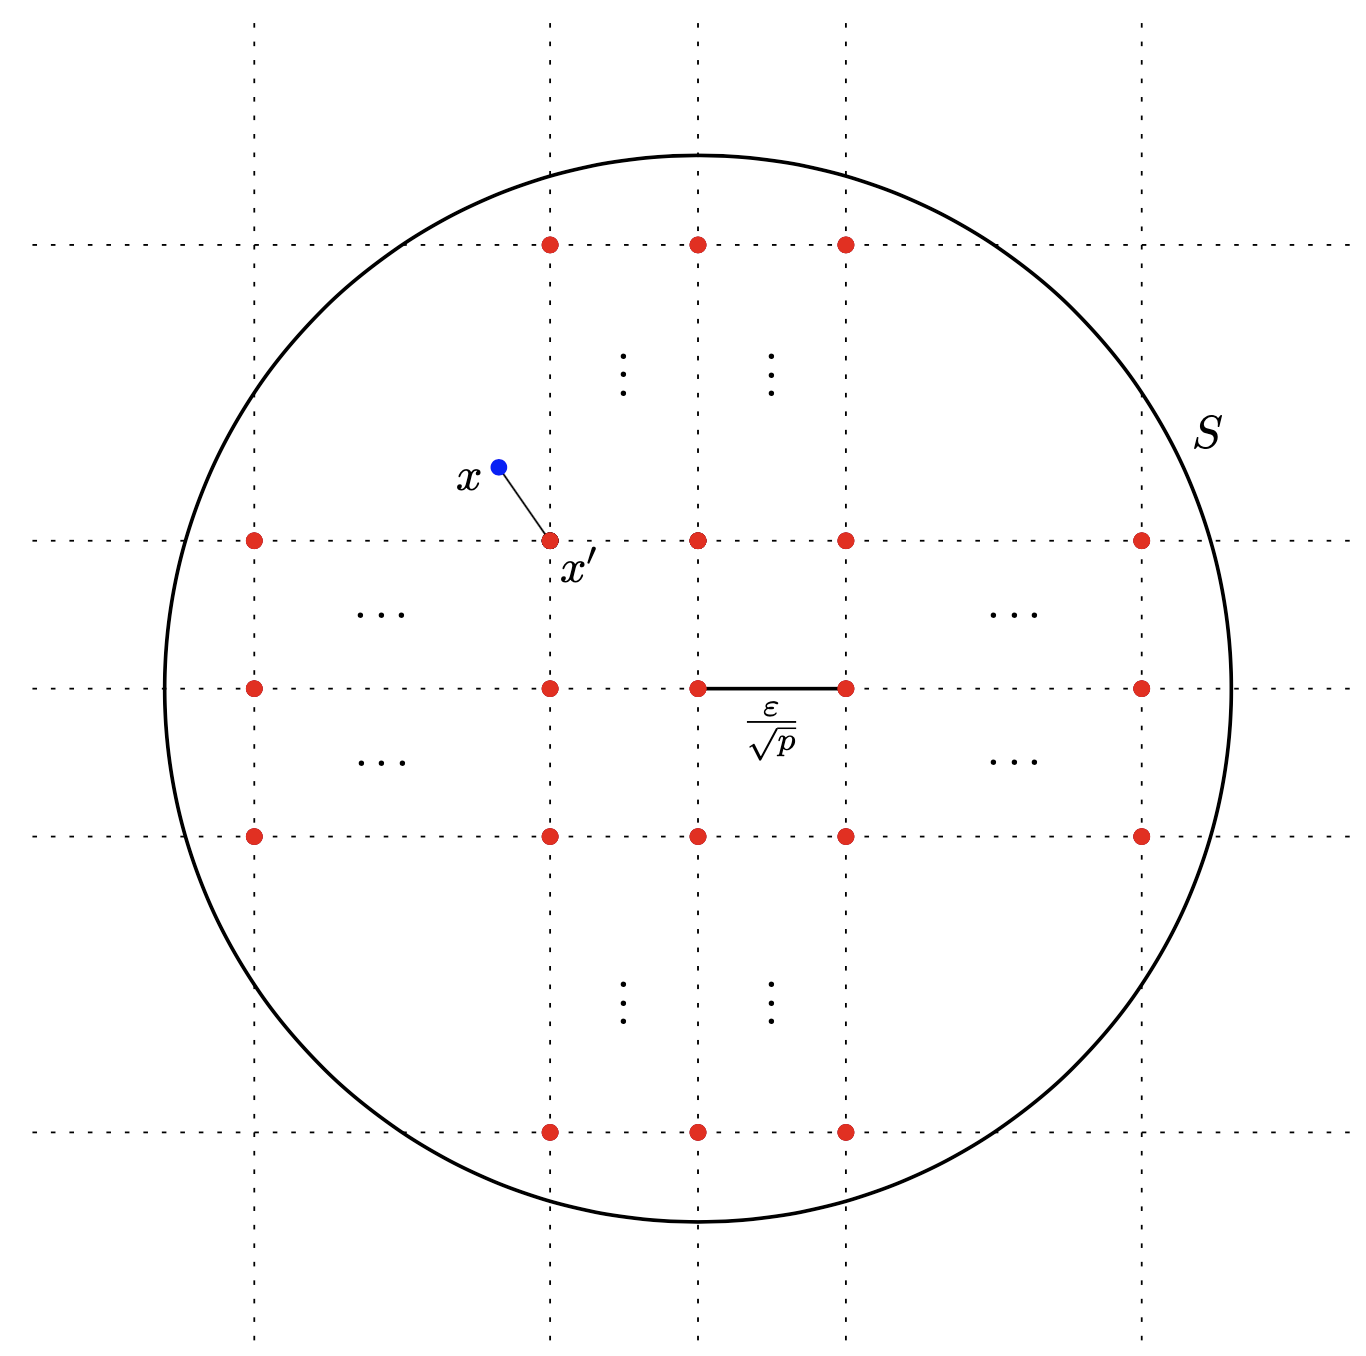
\includegraphics[width=3in]{figures/ECover.png}}
\caption[lec5:fig:ecover]{Our chosen $\epsilon$-cover (shown in red) of $S$. For $x \in S$, we choose the grid point $x'$ such that $\norm{x-x'}_2 \le \epsilon$. \tnoteimp{mention which lemma this figure is for}}
\label{lec5:fig:ecover}
\end{figure}

We claim that $C$ is an $\epsilon$-cover of $S$ with respect to the $\ell_2$-norm: $\forall x \in S$, there exists a grid point $x' \in C$ such that $|x_i-x_i'| \le \tfrac{\epsilon}{\sqrt{p}}$ for each $i$. Therefore,
$$\norm{x-x'}_2 = \sqrt{\sum_{i = 1}^p |x_i - x_i'|^2} \leq \sqrt{p\cdot \frac{\epsilon^2}{p}} = \epsilon.$$

We now bound the size of $C$. Since each $k_i$ in the definition of $C$ has at most $2\tfrac{B\sqrt{p}}{\epsilon}+1$ choices, we have 
\begin{equation}
|C| \le \left( \frac{2B\sqrt{p}}{\epsilon} +1\right)^p \le \left(\frac{3B\sqrt{p}}{\epsilon}\right)^p.
\end{equation}
\end{proof}

\begin{remark}
If $\epsilon > B\sqrt{p}$, then $S$ is contained in the ball centered at the origin with radius $\epsilon$ and the $\epsilon$-cover has size 1.
\end{remark}

\begin{remark}\label{lec4:rem:enet}
We can actually prove a stronger version of Lemma \ref{lec4:lem:ECSize}: there exists an $\epsilon$-cover of $S$ with at most $\left(\frac{3B}{\epsilon}\right)^p$ elements. We will be using this version of the lemma in the proof below. (We will leave the proof of this stronger version as a homework exercise.)
\end{remark}

\subsec{Uniform convergence bound for infinite $\cH$}

\begin{definition}[$\kappa$-Lipschitz functions]
Let $\kappa \ge 0$ and $\norm{\cdot}$ be a norm on the domain $D$. A function $L:D \to \R$ is said to be \emph{$\kappa$-Lipschitz} with respect to $\norm{\cdot}$ if for all $\theta, \theta' \in D$, we have
$$
    |L(\theta)-L(\theta')| \le \kappa \norm{\theta-\theta'}.
$$
\end{definition}

Assume that our infinite hypothesis class $\cH$ can be parameterized by $\cH = \{h_{\theta} : \theta \in \mathbb{R}, \Vert \theta \Vert_2 \leq B\}$. We have the following uniform convergence theorem for our infinite hypothesis class $\cH$:

\begin{theorem}\label{lec4:thm:main}
Suppose $\ell((x,y), \theta) \in [0,1]$, and $\ell((x,y), \theta)$ is $\kappa$-Lipschitz in $\theta$ with respect to the $\ell_2$-norm for all $(x, y)$. Then, with probability  at least $1-O(\exp(-\Omega(p)))$, we have
\begin{equation}
    \forall \theta, \quad |\hat L(\theta)- L(\theta)| \leq  O\left(\sqrt{\frac{p \max(\ln{(\kappa Bn), 1)}}{n}}\right).
\end{equation}
\end{theorem}

\begin{proof}[Proof of Theorem \ref{lec4:thm:main}]
Fix parameters $\delta, \epsilon>0$ (we will specify their values later). Let $C$ be the $\epsilon$-cover of our parameter space $S$ with respect to the $\ell_2$-norm constructed in Lemma \ref{lec4:lem:ECSize}. Define event $E = \left\{ \forall \theta \in C, \; |\hat L(\theta) - L(\theta)| \le \delta \right\}$. By Theorem 4.1, we have $\Pr (E) \ge 1 - 2|C|\exp(-2n\delta^2)$.

Now for any $\theta \in S$, we can pick some $\theta_0 \in C$ such that $\norm{\theta-\theta_0}_2 \le \epsilon$. Since $L$ and $\hatL$ are $\kappa$-Lipschitz functions (this follows from the Lipschitzness of $\ell$), we have
\begin{align}
|L(\theta) - L(\theta_0)| &\le \kappa \norm{\theta-\theta_0}_2 \le \kappa \epsilon, \text{ and} \\
|\hat L(\theta) - \hat L(\theta_0)| &\le \kappa \norm{\theta-\theta_0}_2 \le \kappa \epsilon.
\end{align}

Therefore, conditional on $E$, we have
\begin{equation}
    |\hat L(\theta) -  L(\theta)| \le |\hat L(\theta)-\hat L(\theta_0)| + |\hat L(\theta_0) -  L(\theta_0)| + | L(\theta_0) - L(\theta)| \le 2 \kappa\epsilon+\delta.
\end{equation}

It remains to choose suitable parameters $\delta$ and $\epsilon$ to get the desired bound in Theorem \ref{lec4:thm:main} while making the failure probability small. First, set $\epsilon = \delta / (2 \kappa)$ so that conditional on $E$,
\begin{equation} \label{lec4:eqn:triangle}
    |\hat L(\theta) -  L(\theta)| \le 2\delta.
\end{equation}

If we set $\delta = \sqrt{\frac{c_0 p \max(1, \ln{(\kappa Bn)})}{n}}$ with $c_0 = 36$ (see Remark \ref{lec4:rem:delta} for some intuition), then by Remark \ref{lec4:rem:enet},
\begin{align}
\ln{\vert C \vert} - 2n\delta^2 &\leq p \ln\left(\frac{6B \kappa}{\delta}\right) - 2n\delta^2 \\
&\leq p \ln\left(\frac{6B\kappa \sqrt{n}}{ \sqrt{c_0 p \max(1, \ln{(\kappa Bn)})} }\right) - 2n \frac{c_0p}{n} \ln(\kappa Bn) &(\text{dfn of } \delta)  \\
&\leq p\ln\left(\frac{B\kappa \sqrt{n}}{\sqrt{p}}\right) - 72 p \ln(\kappa Bn) &(\max(1, \ln{(\kappa Bn)}) \geq 1, c_0 = 36) \\
&\leq p \ln(B\kappa n) - 72 p \ln(B\kappa n) &(\sqrt{n/p} \leq n) \\
&\leq -p,
\end{align}
since $\ln (B\kappa n) \geq 1$ for large enough $n$. Therefore, with probability greater than $1 - 2|C| \exp(-2n\delta^2) = 1 - 2 \exp(\ln{|C|} - 2n\delta^2) \geq 1 - O(e^{-p})$, we have
\al{
\vert \hat L(\theta) - L(\theta) \vert \leq 2\delta = O\left(\sqrt{\frac{p}{n}\max(1,\ln(\kappa Bn))}\right).
}
\end{proof}

\begin{remark}\label{lec4:rem:delta}
\sloppy Here is the intuition for the choice of $\delta$: The event $E$ happens with probability $1 - 2|C|\exp(-2n\delta^2) = 1 - 2 \exp(\ln{|C|} - 2n\delta^2)$. From Remark \ref{lec4:rem:enet}, we know that $\ln{|C|} \leq p \ln{ (3B / (\delta / 2)) }$. If we ignore the log term and assume $\ln{|c|} \leq p$, then this would give us the high probability bound we want:
\al{
   2|C| \exp(-2n\delta^2)  = 2\exp(\ln{\vert C \vert} - 2n\delta^2) \leq 2\exp(p - 2p) = 2\exp(-p).
}

(At the same time, we see from \eqref{lec4:eqn:triangle} that this choice of $\delta$ gives $|\hat L(\theta)- L(\theta)| \le 2 \sqrt{\frac{p}{n}}$, which is roughly the bound we want.)

Since we cannot drop the log term in the inequality, we need to make $\delta$ a little big bigger. $\delta$ in the proof was chosen with this intuition in mind to make the subsequent chain of logic work.
\end{remark}

\begin{remark}
We bounded the generalization error $\vert \hat L(\theta) - L(\theta) \vert$ by $\delta + 2\epsilon \kappa \leq \sqrt{\frac{\ln{\vert C \vert}}{n}} + 2\epsilon \kappa$. The term $2\epsilon \kappa$ represents the error from our brute-force discretization. It is not a problem is because we can always choose $\epsilon$ small enough without worrying about the growth of the first term $\sqrt{\frac{\ln{\vert C \vert}}{n}}$. This in turn is because $\ln{\vert C \vert} \approx p\ln{\epsilon^{-1}}$, which is very insensitive to $\epsilon$, even if we let $\epsilon = \frac{1}{poly(n)}$. We also observe that both $\sqrt{\frac{\ln{\vert C \vert}}{n}}$ and $\sqrt{\frac{p}{n}}$ are bounds that depend on the ``size" of our hypothesis class, in terms of either its total size or dimensionality. This possibly explains why one may need more training samples when the hypothesis class is larger.
\end{remark}
	% reset section counter
%\setcounter{section}{0}

%\metadata{lecture ID}{Your names}{date}
\metadata{5}{Will Song}{Jan 27th, 2021}

\sec{Rademacher complexity}

\subsec{Motivation for a new complexity measure}

Recall that our goal is to bound the \textit{excess risk} $L(\hat{h}) - L(h^*)$, where $L$ is the expected loss (or population loss), $\hat{h}$ is our estimated hypothesis and $h^*$ is the hypothesis in the hypothesis class $\cH$ which minimizes the expected loss. We previously showed that to do so it suffices to upper bound $\sup_{h\in \cH} (L (h) - \hatL(h))$. (Note: we often call $L(\hat{h}) - \hatL(\hat{h})$ the \textit{generalization gap} or \textit{generalization error}.)

In the previous sections, we derived bounds for the generalization gap in two cases:
\begin{enumerate}
	\item If the hypothesis class $\cH$ is finite,
	\begin{equation}\label{lec5:eqn:bound-finite}
	L(\hat h) - \hat L(\hat h) \leq \tilde O \l( \sqrt{\frac{\log |\cH|}{n}} \r).
	\end{equation}
	\item If the hypothesis class $\cH$ is $p$-dimensional,
	\begin{equation}\label{lec5:eqn:bound-p}
	L(\hat h) - \hat L(\hat h) \leq \tilde O \l( \sqrt{\frac{p}{n}} \r).
	\end{equation}
\end{enumerate} 
Both of these bounds have a $\frac{1}{\sqrt{n}}$-dependency on $n$, which is known as the ``slow rate". The terms in the numerator ($\log |\cH|$ and $p$ resp.) can be thought of as complexity measures of $\cH$.

The bound \eqref{lec5:eqn:bound-p} is not precise enough: it depends solely on $p$ and is not always optimal. For example, this would be a poor bound if the hypothesis class $\cH$ has very high dimension but small norm. One specific example is for the following two hypothesis classes:
$$ \{\theta : \|\theta\|_1 \leq B\} \qquad \text{vs.} \qquad \{\theta : \|\theta\|_2 \leq B\},$$
\eqref{lec5:eqn:bound-p} would give both hypothesis classes the same bound of $\tilde O \l( \sqrt{\frac{p}{n}} \r)$. Intuitively, we should take into account the norms to prove a better bound.

With the complexity measure to be introduced, we will prove a bound of the form
\begin{align}
    L(\hat h) - \hat L(\hat h) \leq \tilde O\l(\sqrt{\frac{\text{Complexity}(\Theta)}{n}}\r).
\end{align}

This complexity measure will depend on the distribution $P$ over $\cX \times \cY$ (the input and output spaces), and hence takes into account how easy it is to learn $P$. If $P$ is easy to learn, then this complexity measure will be small even if the hypothesis space is big.

One of the practical implications of having such a complexity measure is that we can restrict the hypothesis space by regularizing the complexity measure (assuming it is something we can evaluate and train with). If we successfully find a low complexity model, then this generalization bound guarantees that we have not overfit.

\subsec{Definitions}

In uniform convergence, we sought a high probability bound for $\sup_{h \in H}(L(h) - \hat L (h))$. Here we have a weaker goal: we try to obtain an upper bound for its expectation instead, i.e.
\begin{equation}
\Exp\l[ \sup_{h \in H}(L(h) - \hat L (h)) \r] \leq \text{ upper bound}. \label{lec5:eq:generror}
\end{equation}
The expectation is over the randomness in the training data $\{(x^{(i)}, y^{(i)}\}_{i=1}^n$.\footnote{Though we might like to pull the $\sup$ outside of the $\Exp$ operator, and bound the expectation of the excess risk (a far simpler quantity to deal with!), in general, the $\sup$ and $\Exp$ operators do not commute. In particular, $\Exp\left [\sup_{h \in \cH} (L(h) - \hat{L}(h)) \right ] \geq \sup_{h \in \cH} \Exp \left[ L(h) - \hat{L} (h) \right]$.}

To do so, we first define \textit{Rademacher complexity}.

\begin{definition}[Rademacher complexity] \label{lec5:dfn:rc}
Let $\cF$ be a family of functions mapping $Z \mapsto \bbR$, and let $P$ be a distribution over $Z$. The \textit{(average) Rademacher complexity} of $\cF$ is defined as 
\begin{align}
    R_n(F) \triangleq \Exp_{z_1, \dots, z_n \iid P} \l[ 
    \Exp_{\sigma_1, \dots, \sigma_n \iid\{ \pm 1 \}} \l[ \sup_{f\in F} \frac{1}{n} \sum^n_{i=1} \sigma_i f(z_i) \r] \r], \label{lec5:eqn:Rn}
\end{align}
where $\sigma_1, \dots, \sigma_n$ are independent \textit{Rademacher random variables}, i.e. each taking on the value of $1$ or $-1$ with probability $1/2$.
\end{definition}

\begin{remark}
For applications to empirical risk minimization, we will take $\cZ = \cX \times \cY$. However, Definition \ref{lec5:dfn:rc} holds for abstract input spaces $\cZ$ as well.
\end{remark}

\begin{remark}
Note that $R_n(\cF)$ is also dependent on the measure $P$ of the space, so technically it should be $R_{n,P}(\cF)$, but for brevity, we refer to it as $R_n(\cF)$.
\end{remark}

An interpretation is $R_n(\cF)$ is the maximal possible correlation between outputs of some $f \in \cF$ (on points $f(z_1), \dots, f(z_n)$) and random Rademacher variables $ (\sigma_1, \dots, \sigma_n).$ Essentially, functions with more random sign outputs will better match random patterns of Rademacher variables and have higher complexity (greater ability to mimic or express randomness).

The following theorem is the main theorem involving Rademacher complexity:

\begin{theorem} \label{lec5:thm:thm1}
    \begin{align}
       \Exp_{z_1, \dots, z_n \iid P} \l[ \sup_{f\in F} \l[ \frac{1}{n} \sum^n_{i=1} f(z_i) -  \Exp_{z\sim P} [f(z)] \r]\r] \leq 2 R_n(\cF). \label{lec5:eqn:thm1}
    \end{align}
\end{theorem}

\begin{remark}
We can think of $\frac{1}{n} \sum^n_{i=1} f(z_i)$ as an empirical average and $\Exp_{z\sim P} [f(z)]$ as a population average.
\end{remark}
\noindent\textit{Why is Theorem \ref{lec5:thm:thm1} useful to us?} We can set $\cF$ to be the family of loss functions, i.e.
\begin{equation}
\cF = \l\{ z = (x,y) \in \cZ \mapsto \ell((x,y),h) \in \bbR : h \in \cH \r\}.
\end{equation} 
This is the family of losses induced by the hypothesis functions in $\cH$. We also define the function class $-\cF$ as $\{-f : f \in \cF\}$. It should be obvious from this definition that $R_n(\cF) = R_n(-\cF)$ since $\sigma_i \stackrel{d}{=} -\sigma_i$ for all $i$. Then, letting $z_i = (x^{(i)}, y^{(i)})$,
\begin{align}
    \Exp\l[ \sup_{h \in \cH}\l( L(h) - \hat L (h) \r) \r] &= \Exp_{\{(x^{(i)}, y^{(i)})\}} \l[ \sup_{h \in \cH} \l[L(h) - \frac{1}{n} \sum^n_{i=1} \ell((x^{(i)}, y^{(i)}, h)) \r] \r] \\
    &= \Exp_{\{z_i\}} \l[\sup_{f \in \cF} \l(\Exp[f(z)] - \frac{1}{n} \sum^n_{i=1} f(z_i) \r)\r] \\
    &= \Exp_{\{z_i\}} \l[\sup_{f \in -\cF} \l(\frac{1}{n} \sum^n_{i=1} f(z_i) - \Exp[f(z)] \r)\r] \\
    &\leq 2 R_n(-\cF) = 2R_n(\cF)
\end{align}
where the last step follows by Theorem \ref{lec5:thm:thm1}. 

Thus, $2R_n(\cF)$ is an upper bound for the generalization error. In this context, $R_n(\cF)$ can be interpreted as how well the loss sequence $\ell((x^{(1)}, y^{(1)}), h), \dots \ell((x^{(n)}, y^{(n)}), h)$ correlates with $\sigma_1, \dots, \sigma_n$.
\begin{example}
Consider the binary classification setting where $y \in \{\pm 1\}$. Let $\ell_{0-1}$ denote the zero-one loss function. Note that
\begin{equation}\label{lec5:eqn:01}
    \ell_{0-1}((x,y), h) = \mathbf{1}\{h(x) \neq y\} = \frac{1-yh(x)}{2}.
\end{equation}

Hence,
\begin{align}
    R_n(\cF) &= \Exp_{\{(x^{(i)}, y^{(i)})\}, \sigma_i} \l[ \sup_{h \in \cH} \frac{1}{n}\sum^n_{i=1} \ell_{0-1}((x^{(i)}, y^{(i)}),h)\sigma_i \r] &(\text{by definition}) \\
    &= \Exp_{\{(x^{(i)}, y^{(i)})\}, \sigma_i} \l[ \sup_{h \in \cH} \frac{1}{n}\sum^n_{i=1} \l(\frac{-h(x^{(i)})y^{(i)}+1}{2}\r)\sigma_i \r] &(\text{by } \eqref{lec5:eqn:01}) \\
    &= \frac{1}{2} \Exp_{\{(x^{(i)}, y^{(i)})\}, \sigma_i} \l[ \frac{1}{n}\sum^n_{i=1}\sigma_i + \sup_{h \in \cH} \frac{1}{n}\sum^n_{i=1} -h(x^{(i)})y^{(i)}\sigma_i \r] &(\sup \text{only over } \cH) \\
    &= \frac{1}{2} \Exp_{\{(x^{(i)}, y^{(i)})\}, \sigma_i} \l[\sup_{h \in \cH} \frac{1}{n}\sum^n_{i=1} -h(x^{(i)})y^{(i)}\sigma_i \r] &(\Exp [\sigma_i] = 0) \\
    &=\frac{1}{2} \Exp_{\{(x^{(i)}, y^{(i)})\}, \sigma_i} \l[\sup_{h \in \cH} \frac{1}{n}\sum^n_{i=1} h(x^{(i)})\sigma_i \r] &(-y_i \sigma_i \stackrel{d}{=} \sigma_i) \\
    &= \frac{1}{2}R_n(\cH). &(\text{by definition})
\end{align}

In this setting, $R_n(\cF)$ and $R_n(\cH)$ are the same (except for the factor of 2). $R_n(\cH)$ has a slightly more intuitive interpretation: it represents how well $h \in \cH$ can fit random patterns.

\textbf{Warning!} $R_n(\cF)$ is not always the same as $R_n(\cH)$ in other problems.
\end{example}

\begin{remark}
Rademacher complexity is invariant to translation. This property manifests in the previous example when the $+1$ in the $\l(\frac{-h(x^{(i)})y^{(i)}+1}{2}\r)$ term essentially vanishes in the computation.
\end{remark}

Let us now prove Theorem \ref{lec5:thm:thm1}.

\begin{proof}[Proof of Theorem \ref{lec5:thm:thm1}]
We use a technique called \textit{symmetrization}, which is a very important technique in probability theory. We first fix $z_1, \dots, z_n$and draw $ z_1', \dots z_n' \iid P$. Then we can rewrite the term in the expectation on the LHS of \eqref{lec5:eqn:thm1}:
\begin{align}
    \sup_{f \in \cF} \l( \frac{1}{n} \sum^n_{i=1} f(z_i) - \Exp[f] \r) &= \sup_{f \in \cF} \l( \frac{1}{n} \sum^n_{i=1} f(z_i) - \Exp_{z_1',\dots, z_n'} \l[ \frac{1}{n} \sum^n_{i=1} f(z_i')\r] \r) \\
    &= \sup_{f \in \cF} \l( \Exp_{z_1',\dots, z_n'} \l[\frac{1}{n} \sum^n_{i=1} f(z_i) -  \frac{1}{n} \sum^n_{i=1} f(z_i')\r] \r)\\
    &\leq \Exp_{z_1',\dots, z_n'} \l[\sup_{f \in \cF} \l( \frac{1}{n} \sum^n_{i=1} f(z_i) -  \frac{1}{n} \sum^n_{i=1} f(z_i')\r)\r]. \label{lec5:eqn:thm1-pf1}
\end{align}

The last inequality is because in general,
\begin{align}
    \sup_u \l(\Exp_v[g(u,v)]\r) \leq \sup_u \l( \Exp_v\l[\sup_{u'}g(u',v)\r]\r) = \Exp_v \l[\sup_u (g(u,v))\r]
\end{align}
since the $\sup$ over $u$ becomes vacuous after we replace $u$ with $u'$.

Now, if we take the expectation over $z_1, \dots, z_n$ for both sides of \eqref{lec5:eqn:thm1-pf1},
\begin{align}
    \Exp_{z_1, \dots, z_n} \l[\sup_{f \in \cF} \l( \frac{1}{n} \sum^n_{i=1} f(z_i) - \Exp[f] \r) \r] 
    &\leq \Exp_{z_i} \l[ \Exp_{z_i'} \l[\sup_{f \in \cF} \l( \frac{1}{n} \sum^n_{i=1} \l(f(z_i) -  f(z_i')\r)\r)\r]\r]\\
    &= \Exp_{z_i,z_i'} \l[ \Exp_{\sigma_i} \l[\sup_{f \in \cF} \l( \frac{1}{n} \sum^n_{i=1} \sigma_i\l(f(z_i) -  f(z_i')\r)\r)\r]\r] \label{lec5:eqn:thm1-pf2} \\
 &\leq \Exp_{z_i,z_i', \sigma_i} \l[\sup_{f \in \cF} \l( \frac{1}{n} \sum^n_{i=1} \sigma_i f(z_i)\r)+\sup_{f \in \cF} \l( \frac{1}{n} \sum^n_{i=1} -\sigma_i f(z_i')\r)\r] \\
    &= 2R_n(\cF),
\end{align}
where \eqref{lec5:eqn:thm1-pf2} is because $\sigma_i(f(z_i) - f(z_i')) \stackrel{d}{=} f(z_i) - f(z_i')$ since $f(z_i) - f(z_i')$ has a symmetric distribution. The last equality holds since $-\sigma_i \overset{d}{=} \sigma_i$ and $z_i, z_i'$ are drawn iid from the same distribution. 
\end{proof}

Here is an intuitive understanding of what Theorem \ref{lec5:thm:thm1} achieves. Consider the quantities on the LHS and RHS of \eqref{lec5:eqn:thm1}:
\begin{align*}
    \sup_{f\in \cF} \l(\frac{1}{n} \sum_{i=1}^n f(z_i) - \Exp[f(z)]\r) \qquad \text{v.s.} \qquad \sup_{f\in \cF} \l(\frac{1}{n} \sum_{i=1}^n \sigma_i f(z_i)\r).
\end{align*}
First, we removed $\Exp[f(z)]$, which is hard to control quantitatively since it is deterministic. Second, we added more randomness in the form of Rademacher variables. This will allow us to shift our focus from the randomness in the $z_i$'s to the randomness in the $\sigma_i$'s. In the future, our bounds on the Rademacher complexity will typically only depend on the randomness from the $\sigma_i$'s.

\subsec{Dependence of Rademacher complexity on $P$}
For intuition on how Rademacher complexity depends on the distribution $P$, consider the extreme example where $P$ is a point mass, i.e. $z = z_0$ almost surely. Assume that $-1 \leq f(z_0) \leq 1$ for all $f \in \cF$. Then
\begin{align}
    \Exp_{z_1, \dots, z_n \sim P} \l[ \sup_{f \in \cF} \frac{1}{n} \sum^n_{i=1} \sigma_i f(z_i)\r]
    &= \Exp_{\sigma_1, \dots, \sigma_n} \l[ \sup_{f \in \cF} \frac{1}{n}f(z_0) \sum^n_{i=1} \sigma_i \r] \\
    &\leq \Exp_{\sigma_1, \dots, \sigma_n} \l[ \l| \frac{1}{n} \sum^n_{i=1} \sigma_i \r|\r] &(\text{since } f(z_0) \in [-1,1]) \\
    &\leq \Exp_{\sigma_i} \l[ \l( \frac{1}{n} \sum^n_{i=1} \sigma_i \r)^2\r]^\frac{1}{2} &(\text{Jensen's Inequality}) \\
    &= \frac{1}{n}\l( \Exp_{\sigma_i, \sigma_j} \l[ \sum^n_{i, j=1} \sigma_i\sigma_j \r] \r)^\frac{1}{2}\\
    &= \frac{1}{n}\l( \Exp_{\sigma_i} \l[ \sum^n_{i=1} \sigma_i^2 \r] \r)^\frac{1}{2} \\
    &= \frac{1}{n} \cdot \sqrt{n} = \frac{1}{\sqrt{n}}.
\end{align}
This bound does not depend on $\cF$ (except that it is bounded). This example illustrates that a bound on the Rademacher complexity can sometimes only depend on the (known) distribution of the Rademacher random variables.

\sec{Empirical Rademacher complexity}

In the previous section, we bounded the expectation of $\sup_{f\in F} \l[ \frac{1}{n} \sum^n_{i=1} f(z_i) -  \Exp_{z\sim P} [f(z)] \r]$. This expectation is taken over the training examples $z_1, \dots, z_n$. In many instances we only have one training set, and do not have access to many training sets. Thus, the bound on the expectation does not give a guarantee for the one training set that we have. In this section, we seek to bound the quantity itself with high probability.

\begin{definition}[Empirical Rademacher complexity]
Given a dataset $S = \{z_1, \dots, z_n\}$, the \textit{emprical Rademacher complexity} is defined as
\begin{equation}
R_S(\cF) \overset{\Delta}{=} \Exp_{\sigma_1,\dots, \sigma_n} \l[ \sup_{f\in \cF} \frac{1}{n} \sum^n_{i=1} \sigma_i f(z_i) \r].
\end{equation}
$R_S(\cF)$ is a function of both the function class $\cF$ and the dataset $S$.
\end{definition}

Note that, as the name suggests, the expectation of the empirical Rademacher complexity is the Rademacher complexity:
\begin{align}
    R_n(\cF) = \underset{S=\{z_1,\dots, z_n\}}{\underset{z_1, \dots, z_n \iid P}\Exp}\l[ R_S(\cF) \r].
\end{align}


Here is the theorem involving empirical Rademacher complexity:

\begin{theorem}\label{lec5:thm:thm2}
    Suppose for all $f \in \cF$, $0 \leq f(z) \leq 1$. Then, with probability at least $1-\delta$,
    \begin{align}
        \sup_{f\in \cF} \l[ \frac{1}{n} \sum^n_{i=1} f(z_i) - \Exp[f(z)] \r] \leq 2 R_S(\cF) + 3\sqrt{\frac{\log{(2/\delta)}}{2n}}.
    \end{align}
\end{theorem}

\begin{proof}
For conciseness, define
\begin{equation} g(z_1, \dots, z_n) \triangleq \sup_{f\in F} \l[ \frac{1}{n} \sum^{n}_{i=1} f(z_i) - \Exp[f(z)]\r]. \end{equation}

We prove the theorem in 4 steps.

\textbf{Step 1:} We bound $g$ using McDiarmid's Inequality. To use McDiarmid's inequality, we check that the bounded difference condition holds:
\begin{align}
    g(z_1, \dots, z_n) - g(z_1, \dots, z_i', \dots, z_n)
    &\leq \sup_{f\in \cF} \l[ \frac{1}{n} \sum^{n}_{j=1} f(z_j) \r] - \sup_{f\in \cF} \l[ \l(\frac{1}{n} \sum^{n}_{j=1, j \neq i} f(z_j)\r) + \frac{f(z_i')}{n} \r]  \\
    &\leq \sup_{f\in \cF} \l[ \frac{1}{n} \sum^{n}_{j=1} f(z_j) - \l(\frac{1}{n} \sum^{n}_{j=1, j \neq i} f(z_j)\r) - \frac{f(z_i')}{n} \r] \label{lec5:eqn:thm2-pf1} \\
    &= \sup_{f\in \cF}\l[ \frac{1}{n} \l( f(z_i) - f(z_i') \r) \r] \\
    &\leq \frac{1}{n}. \label{lec5:eqn:thm2-pf2}
\end{align}
\eqref{lec5:eqn:thm2-pf1} holds because in general, $\sup_f A(f) - \sup_f B(f) \leq \sup_f [A(f) - B(f)]$, and \eqref{lec5:eqn:thm2-pf2} holds since $f$ is bounded by $[0,1]$. We can thus apply McDiarmid's Inequality with parameters $c_1 = \dots = c_n = 1/n$:
\begin{align}
    \Pr\l[ g(z_1, \dots, z_n) \geq \Exp_{z_1,\dots, z_n \iid P}[g] + \epsilon \r] \leq \exp{\l( \frac{-2\epsilon^2}{\sum^n_{i=1} c_i^2 }\r)} = \exp(-2n\epsilon^2).
\end{align}

\textbf{Step 2:} We apply Theorem \ref{lec5:thm:thm1} to get 
\begin{align}
 \Exp_{z_1,\dots, z_n \iid P}[g] \leq 2R_n(\cF).
\end{align}

\textbf{Step 3:} Define
\begin{equation} \tilde g (z_1, \dots, z_n) = R_S(\cF) \triangleq \Exp_{\sigma_i}\l[\sup_{f\in \cF} \frac{1}{n} \sum^n_{i=1} \sigma_i f(z_i)\r]. \end{equation}

Using a similar argument to that of Step 1, we show that $\tilde g$ satisfies the bounded difference condition:
\begin{align}
    &\tilde g(z_1, \dots, z_n) - \tilde g(z_1, \dots, z_i', \dots, z_n) \nonumber \\
    &\leq \Exp_{\sigma_i} \l[\sup_{f\in F} \l[ \frac{1}{n} \sum^{n}_{j=1} \sigma_j f(z_j) \r] - \sup_{f\in F} \l[ \l(\frac{1}{n} \sum^{n}_{j=1, j \neq i} \sigma_j f(z_j)\r) + \frac{1}{n} \sigma_if(z_i')\r]\r]\\
    &\leq \Exp_{\sigma_i}\l[\sup_{f\in F} \l(\frac{1}{n} \sigma_i(f(z_i) - f(z_i'))\r)\r] \\
    &\leq \frac{1}{n},
\end{align}
since the term inside the $\sup$ is always upper bounded by 1. We can thus apply McDiarmid's Inequality with parameters $c_1 = \dots = c_n = 1/n$:
\begin{align}
    \Pr\l[ \tilde g - \Exp[\tilde g] \geq \epsilon \r] \leq \exp(-2n \epsilon^2), \quad\text{and}\quad
    \Pr\l[ \tilde g - \Exp[\tilde g] \leq -\epsilon \r] \leq \exp(-2n \epsilon^2).
\end{align}

\textbf{Step 4:} We set $\delta$ such that $\exp(-2n \epsilon^2) = \delta/2$. (This implies that $\epsilon = \sqrt{\frac{\log(2/\delta)}{2n}}$.) Then, with probability $\geq 1 - \delta$,
\begin{align}
    \sup_{f\in \cF} \l[ \frac{1}{n} \sum^n_{i=1} f(z_i) - \Exp[f]\r] = g &\leq \Exp[g] + \epsilon &\text{(Step 1)} \\
    &\leq 2R_n(\cF) + \epsilon &\text{(Step 2)} \\
    &\leq 2(R_S(\cF) + \epsilon) + \epsilon &\text{(Step 3)} \\
    &= 2R_S(\cF) + 3\epsilon,
\end{align}
as required.
\end{proof}

Setting $\cF$ to be a family of loss functions bounded by $[0,1]$ in Theorem \ref{lec5:thm:thm2} gives the following corollary:
\begin{corollary}\label{lec6:cor:ggap-rsbound}
Let $\cF$ to be a family of loss functions $\cF = \l\{ (x,y) \mapsto \ell((x,y),h): h \in \cH \r\}$ with $\ell((x,y), h) \in [0,1]$ for all $\ell$, $(x,y)$ and $h$. Then, with probability $1-\delta,$ the generalization gap is
    \begin{equation}\label{lec6:eqn:ggap-rsbound}
        \hat{L}(h) - L(h) \leq 2R_S(\cF) + 3\sqrt{\frac{\log(2/\delta)}{2n}} \quad \text{for all } h\in \cH.
    \end{equation}
\end{corollary}

\begin{remark}
If we want to bound the generalization gap by the average Rademacher complexity instead, we can replace the RHS of \eqref{lec6:eqn:ggap-rsbound} with $2R_n(\cF) + \sqrt{\frac{\log(2/\delta)}{2n}}$.
\end{remark}

\paragraph{Interpretation of  Corollary \ref{lec6:cor:ggap-rsbound}.}
\sloppy It is typically the case that $O\l(\sqrt{\frac{\log (2/\delta)}{n}}\r) \ll R_S(\cF)$ and $O\l(\sqrt{\frac{\log (2/\delta)}{n}}\r) \ll R_n(\cF)$. This is the case because $R_S(\cF)$ and $R_n(\cF)$ often take the form $\frac{c}{\sqrt{n}}$ where $c$ is a big constant depending on the complexity of $\cF$, whereas we only have a logarithmic term in the numerator of $O\l(\sqrt{\frac{\log (2/\delta)}{n}}\r)$. As a result, we can view the $3\sqrt{\frac{\log (2/\delta)}{n}}$ term in the RHS of Corollary \ref{lec6:cor:ggap-rsbound} as negligible. Another way of seeing this is noting that a $\tilO \left( \frac{1}{\sqrt{n}} \right)$ term is necessary even for the concentration bound of a single function $h\in\cH$. Previously, we bounded $L(h)-\hat{L}(h)$ using a union bound over $h\in\cH$, which necessarily needs to be larger than $\tilO \left(\frac{1}{\sqrt{n}} \right)$. As a result, the $O\l(\sqrt{\frac{\log (2/\delta)}{n}}\r)$ term is not significant.

%\subsec{Empirical Rademacher complexity viewed in the output/function space}
%Assume we have a fixed dataset $S = \{z_1, \dots, z_n\}$. Since $z_1,\dots, z_n$ is fixed, each function $f\in\cF$ corresponds to a single output $(f(z_1),\dots,f(z_n))\in \R^n$. Hence, we can express the set of outputs for every function $f\in\cF$ as
%\begin{align}
%    Q_\cF = \left\{ \begin{pmatrix}f(z_1), \dots, f(z_n) \end{pmatrix} \mid f\in\cF \right\}.
%\end{align}
%
%Now we can mathematically re-express the empirical Rademacher complexity as an inner product:
%\begin{align}
%R_S(\cF) &= \Exp_{\sigma_1,\dots, \sigma_n} \l[ \sup_{f\in \cF} \frac{1}{n} \sum^n_{i=1} \sigma_i f(z_i) \r] \\
%&= \Exp_{\sigma_1,\dots, \sigma_n} \l[ \sup_{v\in Q} \frac{1}{n}\langle\sigma, v\rangle \r],
%\end{align}
%where $\sigma=(\sigma_1,\dots,\sigma_n)$. (See Figure \ref{lec6:fig:rs-innerprod} for an illustration of this idea.) This perspective will be helpful later on when proving bounds on the empirical Rademacher complexity.




\subsec{Rademacher complexity is translation invariant}
A useful fact is that both empirical Rademacher complexity and average Rademacher complexity are translation invariant. (This is not obvious when thinking of how translation affects the picture in Figure \ref{lec6:fig:rs-innerprod}.)

\begin{proposition}
Let $\cF$ be a family of functions mapping $Z \mapsto \R$ and define $\cF' = \{f'(z) = f(z) + c_0\mid f\in \cF\}$ for some $c_0\in\R$. Then $R_S(\cF) = R_S(\cF')$ and $R_n(\cF) = R_n(\cF')$.
\end{proposition}

\begin{proof}
We will prove here that empirical Rademacher complexity is translation invariant.
\begin{align}
R_S(\cF') &= \Exp_{\sigma_1,\dots, \sigma_n} \l[ \sup_{f'\in \cF'} \frac{1}{n} \sum^n_{i=1} \sigma_i f(z_i) \r] \\
&= \Exp_{\sigma_1,\dots, \sigma_n} \l[ \sup_{f\in \cF} \frac{1}{n} \sum^n_{i=1} \sigma_i (f(z_i)+c_0) \r] \\
&= \Exp_{\sigma_1,\dots, \sigma_n} \l[ \frac{1}{n} \sum^n_{i=1} \sigma_i c_0 + \sup_{f\in \cF} \frac{1}{n} \sum^n_{i=1} \sigma_i f(z_i) \r] \\
&= \Exp_{\sigma_1,\dots, \sigma_n} \l[\sup_{f\in \cF} \frac{1}{n} \sum^n_{i=1} \sigma_i f(z_i) \r] = R_S(\cF), \label{lec6:eqn:rs-translation}
\end{align}
where \eqref{lec6:eqn:rs-translation} follows because $\Exp_{\sigma_1,\dots,\sigma_n} \frac{1}{n}\sum_{i=1}^n \sigma_i c_0 = 0$, since the $\sigma_i$'s are Rademacher random variables.
\end{proof}


	 % reset section counter
%\setcounter{section}{0}
\metadata{8}{David Lin and Jinhui Wang}{Feb.~8th, 2021}

\sec{Covering number upper bounds Rademacher complexity}
In Chapter \ref{chap:gen-bounds}, we will prove Rademacher complexity bounds that hinge on elegant, ad-hoc algebraic manipulations that may not extend to more general settings. Here, we consider a more fundamental approach for proving empirical Rademacher complexity bounds based on coverings of the output space. The trade-off is generally more tedium.

The first important observation is that for purposes of computing the \textbf{empirical} Rademacher complexity on samples $z_1, ..., z_n$, 
\al{
    R_S(\cF) = \Exp_\sigma \sbr{\sup_{f \in \cF} \frac 1 n \sum_{i=1}^n \sigma_i f(z_i)},
}
we only care about the output of function $f \in \cF$, and not the function itself (i.e. it is sufficient for our purposes to know $f(z_1),\dots, f(z_n)$, but not know $f$). In other words, we can characterize $f \in \cF$ by $f(z_1),\dots, f(z_n)$. In the sequel, we will take advantage of this simplification from the (potentially large) space of all functions $\cF$ to the \textit{output space},
\begin{equation}
\cQ \triangleq \cbr{ \begin{pmatrix} f(z_1), \dots, f(z_n) \end{pmatrix}^\top: f\in \cF} \subseteq \R^n, \label{lec6:eqn:shattercoef}
\end{equation}
which may be drastically smaller than $\cF$. Correspondingly, the empirical Rademacher complexity can be rewritten as a maximization over the output space $\cQ$ instead of the function space $\cF$: 
\al{
    R_S(\cF) &= \Exp_\sigma \sbr{\sup_{v\in \cQ} \frac 1 n \inprod{\sigma, v}}.
}
In other words, the complexity of $\cF$ can be also interpreted as how much the vectors in $Q$ can be correlated with a random vector $\sigma.$ See Figure \ref{lec6:fig:rs-innerprod} for an illustration of this idea. One can also view $\Exp_\sigma \sbr{\sup_{v\in \cQ} \frac 1 n \inprod{\sigma, v}}$ as a complexity measure for the set $Q$. If we replace $\sigma$ by a Gaussian vector with spherical covariance, then the corresponding quantity (without the $\frac 1 n$ scaling), $\Exp_{g\sim N(0,I)} \sbr{\sup_{v\in \cQ} \inprod{g, v}}$, is often referred to as the Gaussian complexity of the set $Q$. (It turns out that Gaussian complexity and Rademacher complexity are closely related.)

Another corollary of this is that the empirical Rademacher complexity only depends on the functionality of $\cF$ but not on the exact parameterization of $\cF$ . For example, suppose we have two parameterizations $\cF = \left\{f(x)=\sum \theta_{i} x_{i} \mid \theta \in \mathbb{R}^{d}\right\}$ and $\cF' = \left\{f(x)=\sum \theta_{i}^{3} \cdot w_{i} x_{i} \mid \theta \in \R^{d}, w \in \mathbb{R}^{d}\right\}$. Since $Q_\cF$ and $Q_{\cF'}$ are the same, we see that $R_S(\cF) = R_S(\cF')$ since our earlier expression for $R_S(\cF)$ only depends on $\cF$ through $Q_\cF$. 

\begin{figure}[ht!]
	\begin{center}
		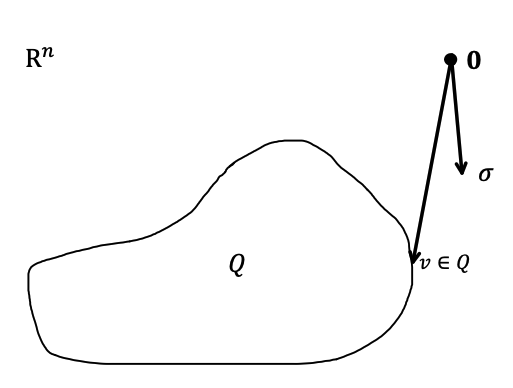
\includegraphics[width=.5\textwidth]{figures/remark2.png}
	\end{center}
	\caption{We can view empirical Rademacher complexity as the expectation of the maximum inner product between $\sigma$ and $v\in Q$.}
	\label{lec6:fig:rs-innerprod}
\end{figure}

\paragraph{Rademacher complexity of finite hypothesis classes.} In practice, we cannot directly evaluate the Rademacher complexity, so we instead bound its value using quantities that are computable. Given finite $|\cQ|$, we often rely on the following bound, which is also known as Masssart's finite lemma: 
\begin{proposition}
    Let $\cF$ be a collection of functions mapping $Z \mapsto \mathbb{R}$ and let $\cQ$ be defined as in \eqref{lec6:eqn:shattercoef}. Assume that $\frac{1}{\sqrt{n}} \norm{v}_2 \le M < \infty$ for all $v \in \cQ$. Then,
    \begin{align}
        R_S(\cF) \leq \sqrt{\frac{2 M^2 \log |\cQ|}{n}}
    \end{align}
    \label{lec6:prop:massartlemma}
\end{proposition}
We prove a (slightly) simplified version of this result in Problem 3(c) of Homework 2, so we omit the proof of Massart's lemma here. 

\begin{remark}
    Using Massart's lemma, we can bound the Rademacher complexity without referring to $\cQ$. Restating the assumption accordingly, we observe that if $\sqrt{\frac{1}{n}\sum_{i=1}^n f(z_i)^2} \le M$ for all $f \in \cF$, then $R_s(\cF) \le \sqrt{\frac{2M^2\log \abs{\cF}}{n}}$. Note that this corollary yields a looser bound than Massart's lemma since $|\cQ| \leq |\cF|$. 
\end{remark}
    
In practice, we rarely apply Massart's lemma directly since $|\cQ|$ is typically infinite. In the sequel, we discuss alternative approaches to bounding the Rademacher complexity that are appropriate for this setting.

\paragraph{Bounding Rademacher complexity using $\epsilon$-covers.}
When $|\cQ|$ is infinite, we can apply the same discretization trick that we used to prove the generalization bound for an infinite-hypothesis space. This time, instead of trying to cover the parameter space, we will cover the output space. To this end, we first recall a few definitions concerning $\epsilon$-covers.

\begin{definition}
$\cC$ is an \emph{$\epsilon$-cover} of $\cQ$ with respect to metric $\rho$ if for all $v' \in \cQ$, there exists $v \in \cC $ such that $\rho(v,v')\le \epsilon$.
\end{definition}

\begin{definition}
The \emph{covering number} is defined as the minimum size of an $\epsilon$-cover, or explicitly:
\begin{align}
    N(\epsilon, \cQ, \rho) \overset \triangle = (\text{min size of $\epsilon$-cover of $\cQ$ w.r.t.\ metric $\rho$}).
\end{align}
\end{definition}

\begin{figure}[h]
	\begin{center}
		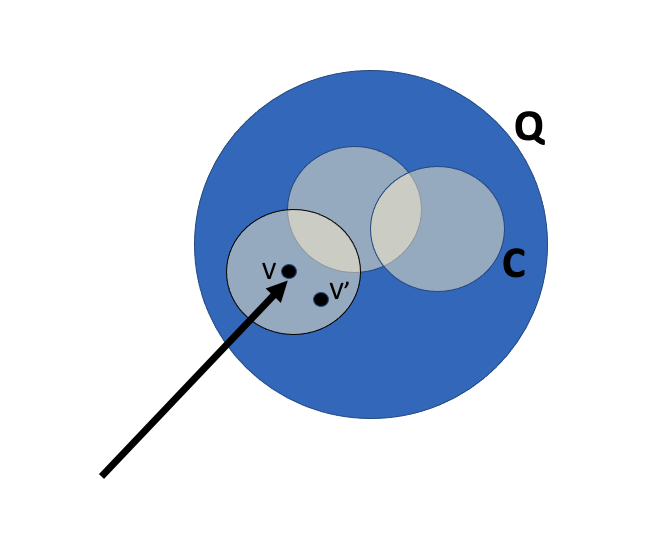
\includegraphics[width=.5\textwidth]{figures/onestep_bound.png}
	\end{center}
	\caption{We can visualize the $\epsilon$-cover $\cC$ by depicting a set of $\epsilon$-balls that cover the output space $\cQ$. The yellow circles denote the $\epsilon$-neighborhoods of the covering points $v \in \cC$.}
	\label{lec9:fig:eps-cover}
\end{figure}

In subsequent derivations, we will use the metric $\rho(v,v') = \frac 1 {\sqrt{n}} \norm{v-v'}_2$. 

\begin{remark}
We normalize the $\ell_2$ norm in $\rho$ by $\frac{1}{\sqrt{n}}$ to simplify comparisons to the functional analysis view of the Rademacher complexity. In the literature, the $\epsilon$-cover of $\cQ$ defined above is also referred to as an $\epsilon$-cover of the function class $\cF$ under the $L_2[P_n]$ metric.\footnote{$P_n$ denotes the empirical distribution, i.e. the uniform distribution over the observations $z_1,\dots,z_n$. More generally the $L_p[Q]$ metric is defined by $\Exp_Q \left [\left (f(z) - f'(z) \right )^p \right]^{1/p}$.} In particular, 
\begin{align}
L_2[P_n](f,f') = \sqrt{ \frac 1 n \sum_{i=1}^n (f(z_i) - f'(z_i))^2 }.
\end{align}
Recall we have established the following correspondences between the set of functions $\cF$ and the output space $\cQ$:
\begin{align}
    f \in \cF \iff \begin{pmatrix} f(z_1) \\ \vdots \\ f(z_n) \end{pmatrix} \in \cQ
\end{align}

We can write a trivial correspondence between both the output and function class points of view as follows:
\begin{align}
N(\epsilon, \cF, L_2(P_n)) = N\left (\epsilon, \cQ, \frac{1}{\sqrt{n}} || \cdot ||_2 \right )
\end{align}
The results below will be stated in the function-space notation, but in the proofs we will shift to the $\cQ$-formulation for the sake of clarity.
In general, we prefer to reason about covering numbers on $\cQ$ as it is more natural to analyze vector spaces compared to function spaces.
\label{lec8:rmk:l2pncover}
\end{remark}

Equipped with the definition of minimal $\epsilon$-covers, we can prove the following Rademacher complexity bound:

\begin{theorem}\label{lec8:thm:rc-covering-bd}
Let $\cF$ be a family of functions $Z \mapsto [-1,1]$. Then
\begin{equation}
R_S(\cF) \le \inf_{\epsilon > 0} \rbr{ \epsilon + \sqrt{ \frac {2\log N(\epsilon, \cF, L_2[P_n])} n } }. \label{lec8:eqn:rc-covering-bd}
\end{equation}
\end{theorem}

The $\epsilon$ term can be thought of as the discretization error, while the second term follows from Proposition~\ref{lec6:prop:massartlemma}.

\begin{proof}
Fix any $\epsilon > 0$. Let $\cC$ be the minimal $\epsilon$-cover $\cC$ of $\cQ$ with respect to the metric $\rho(v,v') = \frac 1 {\sqrt{n}} \norm{v-v'}_2$. 

For every point $v\in \cQ$, $v=v'+z$, where $v'\in \cC$ and $z$ is small (specifically, $\frac 1 {\sqrt{n}} \norm{z}_2 \le \epsilon$). This gives
\al{
    \frac 1 n \inprod{v, \sigma} &= \frac 1 n \inprod{v',\sigma} + \frac 1 n \inprod{z, \sigma}\\
    &\le \frac 1 n \inprod{v', \sigma} + \frac 1 n \norm{z}_2 \norm{\sigma}_2 
        &&\text{(Cauchy-Schwarz)} \label{lec8:eqn:cs-step}\\
    &\le \frac 1 n \inprod{v', \sigma} + \epsilon.
        &&\text{(since $\norm{z}_2\le \sqrt{n}\epsilon$ and $\norm{\sigma}_2 \le \sqrt{n}$)}
}
Taking the expectation of the supremum on both sides of this inequality gives
\al{
    R_S(\cF) &= \Exp_\sigma \sbr{\sup_{v\in \cQ} \frac 1 n \inprod{v,\sigma} }\\
    &\le \Exp_\sigma \sbr{\sup_{v'\in \cC} \rbr{\frac 1 n \inprod{v',\sigma} + \epsilon}}\\ 
    &\le \epsilon + \sqrt{ \frac {2\log \abs{\cC}} n } &\text{(Proposition~\ref{lec6:prop:massartlemma})} \\
    &= \epsilon + \sqrt{ \frac {2\log N(\epsilon, \cQ , \rho)} n } \\
    &= \epsilon + \sqrt{ \frac {2\log N(\epsilon, \cF , L_2[P_n])} n } &\text{(Remark~\ref{lec8:rmk:l2pncover})}
}
Since the argument above holds for any $\epsilon > 0$, we can take the infimum over all $\epsilon$ to arrive at Equation \eqref{lec8:eqn:rc-covering-bd}.

\end{proof}

\sec{Chaining and Dudley's theorem}

While Theorem \ref{lec8:thm:rc-covering-bd} is useful, the bound in Equation \eqref{lec8:eqn:cs-step} is rarely tight as $z$ might not be perfectly correlated with $\sigma$. It is possible to obtain a stronger theorem by constructing a chained $\epsilon$-covering scheme. Specifically, when we decompose $v=v'+z$, we can construct a finer-grained covering of the ball $B(v',\epsilon)$, and then we can decompose $z$ into smaller components and so on (see Figure \ref{lec9:fig:chaining_diag} for an illustration).

Using this method of chaining, we can obtain the following (stronger) result:

\begin{theorem}[Dudley's Theorem]
If $\cF$ is a function class from $Z$ to $\R$, then
\begin{equation}
    R_S(\mathcal{F})\leq 12\int_{0}^{\infty}\sqrt{\frac{\log N(\epsilon, \mathcal{F}, L_2[P_n])}{n}}d\epsilon. \label{lec9:eqn:dudley}
\end{equation}
\end{theorem}

Note that this theorem does not require the functions to be bounded.

\begin{remark}

It is not obvious how \eqref{lec9:eqn:dudley} improves upon the one-step discretization bound given by \eqref{lec8:eqn:rc-covering-bd}. At a high level, we can interpret this bound as removing the discretization error term by averaging over different scales of $\epsilon$.  But before we can explicitly prove this claim, we motivate our approach. In the proof of Theorem~\ref{lec8:thm:rc-covering-bd}, we approximated $v$ with $v' + z$ where $v'$ is the closest point to $v$ in the minimal $\epsilon$-cover of $\cQ$, and $z$ is the vector between $v'$ and $v$. In particular,
\begin{equation}
    \frac 1 n \inprod{v, \sigma} = \frac 1 n \inprod{v', \sigma} + \frac 1 n \inprod{z, \sigma} \label{lec9:eqn:disc_decomp}
\end{equation}
The difficult term to deal with is the last one, $\frac 1 n \inprod{z, \sigma}$. In the previous derivation, we naively upper bounded $\inprod{z, \sigma}$ using Cauchy-Schwarz,
\begin{equation}
    \frac 1 n \inprod{z,\sigma} \le \frac{\norm{z}_2\cdot \norm{\sigma}_2} n,
\end{equation}
but this bound is only tight if $z$ is perfectly correlated with $\sigma$. We claim that such perfect correlation is unlikely. Recall that the output space is defined by possible outputs of $f \in \cF$ given $n$ inputs. Unless our function class is extremely expressive, the set of radius $\epsilon$ around $v'$ contained in $\cQ$ will only be a small subset of the $\epsilon$-ball centered at $v'$; thus, $\sup_{z} \frac{1}{n} \inprod{z, \sigma} \ll \frac{\norm{z}_2 \cdot \norm{\sigma}_2}{n}$.

To more tightly bound $\Exp \l[ \sup \frac 1 n \inprod{z,\sigma}\r]$, we repeat the $\epsilon$-covering argument again with a smaller choice of $\epsilon$. Intuitively, this  procedure amounts to decomposing $\inprod{z, \sigma}$ from \eqref{lec9:eqn:disc_decomp} into another pair of terms corresponding to the new $\epsilon$-cover and the discretization error. ``Chaining'' then repeats this decomposition countably many times. Putting this argument in terms of Rademacher complexity, we can think of each chaining iteration as bounding $R_S(B_{v} \cap \cQ)$ where $B_{v}$ denotes the $\epsilon$-ball around $v \in \cC$ for the $\epsilon$-cover $\cC$ defined in the previous iteration. This procedure is illustrated visually by Figure~\ref{lec9:fig:chaining_diag}, and we formalize this argument in the sequel.
\end{remark}

\begin{figure}[ht!]
    \centering
    \begin{subfigure}[t]{0.45\textwidth}
        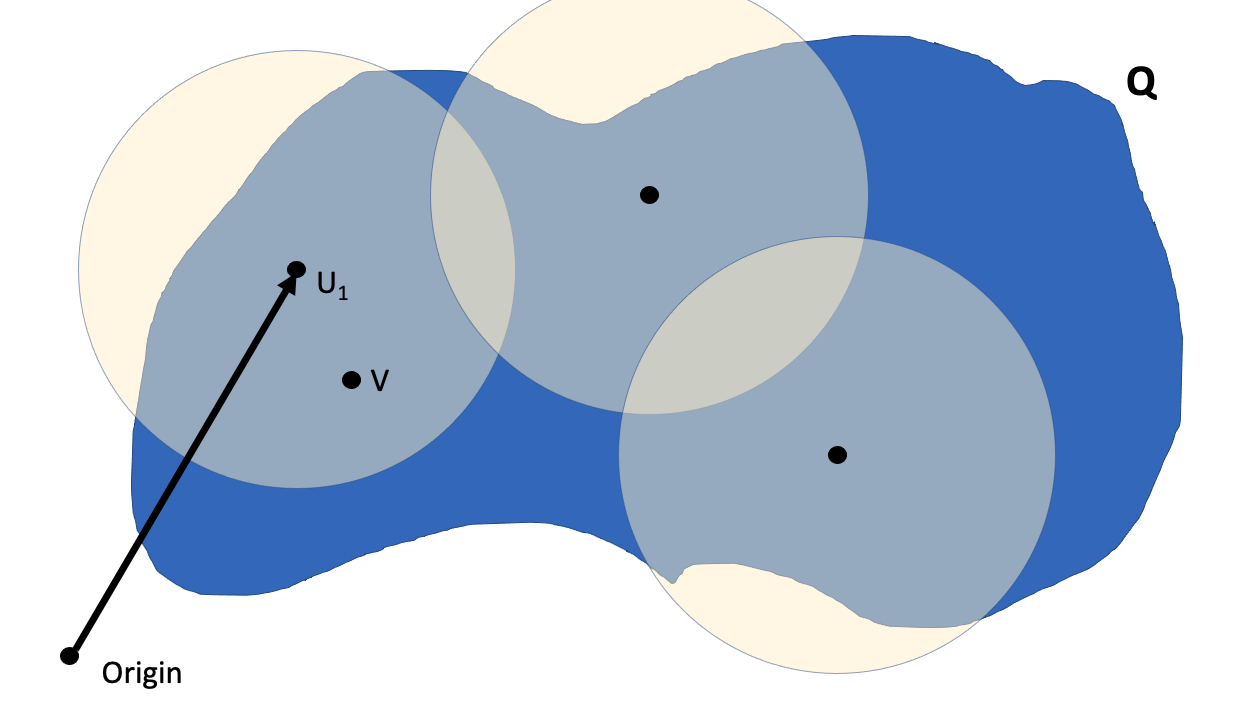
\includegraphics[width=\textwidth]{figures/chaining_1.png}
        \caption{}
        \label{lec9:fig:chaining_1}
    \end{subfigure}
    \hfill
    \begin{subfigure}[t]{0.45\textwidth}
        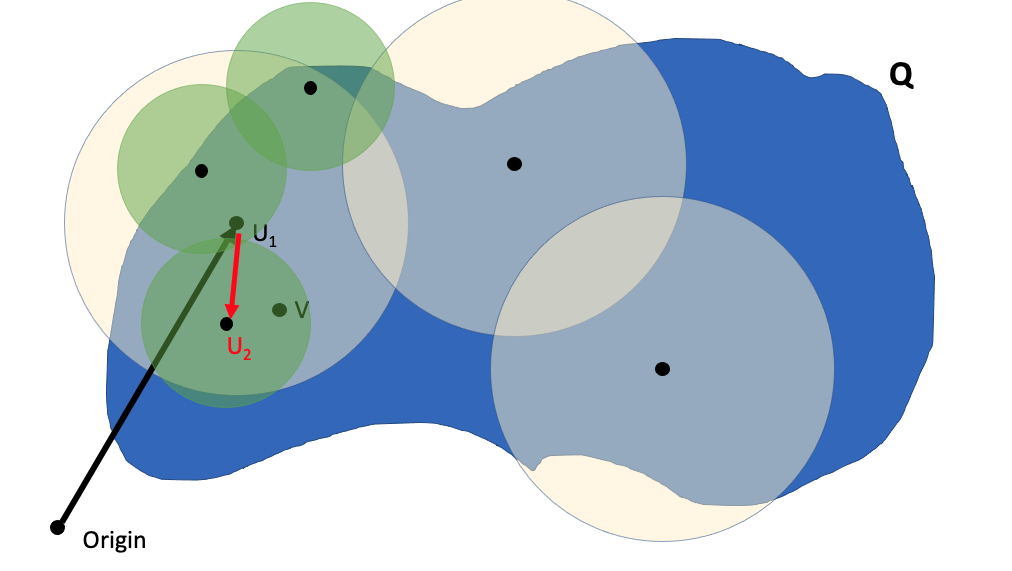
\includegraphics[width=\textwidth]{figures/chaining_2.png}
        \caption{}
        \label{lec9:fig:chaining_2}
    \end{subfigure}
    \hfill
    \begin{subfigure}[t]{0.45\textwidth}
        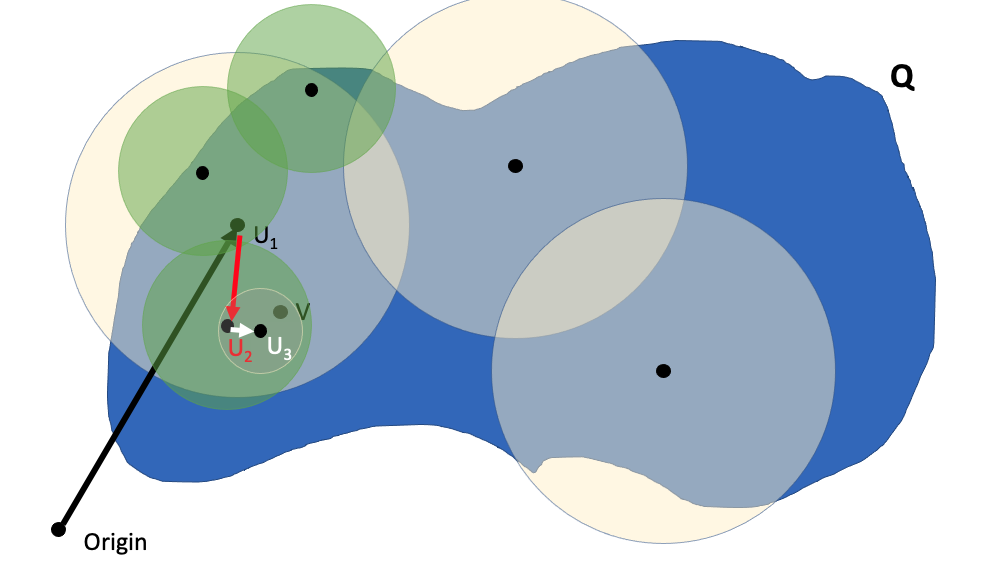
\includegraphics[width=\textwidth]{figures/chaining_3.png}
        \caption{}
        \label{lec9:fig:chaining_3}
    \end{subfigure}
    \caption{We depict how the chaining procedure approximates $v$ using a sequence of progressively finer discretizations. Figure~\ref{lec9:fig:chaining_1} illustrates how we first approximate $v$ using the nearest covering point $u_1$, while Figures~\ref{lec9:fig:chaining_2} and \ref{lec9:fig:chaining_3} describe how we refine this approximation using two finer covers, whose nearest points are denoted by $u_2$ and $u_3$, respectively.}
    \label{lec9:fig:chaining_diag}
\end{figure}

\begin{proof} 
    Let $\epsilon_0 = \sup_{f\in \cF} \max_i \abs{f(z_i)}$, so that $\forall v \in \cQ$,
    \begin{equation}
        \epsilon_0 \ge \sqrt{\frac 1 n \sum_{i=1}^nf(z_i)^2}  = \sqrt{\frac 1 n \sum_{i=1}^n \norm{v}_2^2}.
    \end{equation}
    
    Define $\epsilon_1 = 2^{-1}\epsilon_0, \epsilon_2 = 2^{-2}\epsilon_0, \epsilon_j = 2^{-j}\epsilon_0$ and let $\cC_j$ be an $\epsilon_j$-cover of $\cQ$. Then, $\cC_0$ is the coarsest cover of $\cQ$, and as $j$ increases, we obtain progressively more fine-grained covers $\cC_j$.
    
    We use this sequence of covers to define a telescoping series that equals $v$ whose terms can be analyzed using tools that we have developed in the prequel. In particular, for $v \in \cQ$, let $\pi_i(v)$ denote the nearest neighbor of $v$ in $\cC_i$. Taking $\pi_0(v) = 0$, it follows from our definition of $\cC_i$ that
    \begin{align}
        v &= \pi_1(v) + \sum_{i = 2}^\infty (\pi_i(v) - \pi_{i - 1}(v)) \\
        &= \sum_{i = 1}^\infty (\pi_i(v) - \pi_{i - 1}(v)).
    \end{align}
    
    By definition, $\rho(v, \pi_i(v)) \le \epsilon_i$ and thus $\frac 1 {\sqrt n} \norm{v - \pi_i(v)}_2 \le \epsilon_i$. Examining our previous expression of interest, 
    \al{
        \Exp\l[\sup_{v \in \cQ} \frac 1 n \inprod{v, \sigma}\r]&= \Exp\l[\sup_{v \in \cQ} \frac 1 n \sum_{i=1}^\infty \inprod{\pi_i(v)-\pi_{i - 1}(v), \sigma}\r]\\
        &\le \Exp\l[\sum_{i=1}^\infty \sup_{u_i \in \cC_i, u_{i - 1} \in \cC_{i - 1}} \frac 1 n\inprod{u_i - u_{i - 1}, \sigma}\r]\\
        &= \sum_{i=1}^\infty \Exp\l[ \sup_{u_i \in \cC_i, u_{i - 1} \in \cC_{i - 1}} \frac 1 n\inprod{u_i - u_{i - 1}, \sigma}\r]. \label{lec9:eqn:chaining_expansion}
    }
    Observe that
    \begin{equation}
        \Exp\l[ \sup_{u_i \in \cC_i, u_{i - 1} \in \cC_{i - 1}} \frac 1 n\inprod{u_i-u_{i - 1}, \sigma}\r]
    \end{equation}
    is a Rademacher complexity defined over the \emph{finite} space $\cC_i \times \cC_{i - 1}$, so we can use Massart's lemma to obtain a tractable upper bound. To do so, we must first compute an upper bound on $\frac{1}{\sqrt{n}} \norm{u_i - u_{i - 1}}_2$, i.e. compute $M$ from Proposition~\ref{lec6:prop:massartlemma}:
    \al{
        \frac 1 {\sqrt n} \norm{u_i - u_{i - 1}}_2 &= \frac 1 {\sqrt{n}} \norm{(u_i - v) - (u_{i - 1} - v)}_2\\
        &\le \frac 1 {\sqrt{n}} \l(\norm{u_i - v}_2 - \norm{u_{i - 1} - v}_2 \r)\\
        &\le \epsilon_i + \epsilon_{i - 1} \\
        &= 3 \epsilon_i & \text{($\epsilon_{i - 1} \defeq 2 \epsilon_i$)}
    }
    Now we apply Proposition~\ref{lec6:prop:massartlemma} with $M = 3 \epsilon_i$ and $\abs{\cQ} = \abs{\cC_i \times \cC_{i - 1}} \leq \abs{\cC_i} \cdot \abs{\cC_{i - 1}}$.
    \al{
        \Exp\l[\sup_{u_i \in \cC_i, u_{i - 1} \in \cC_{i - 1}} \frac 1 n \inprod{u_i - u_{i - 1}, \sigma} \r] & \le \sqrt{\frac{2(3 \epsilon_i)^2\log (\abs{\cC_i}\cdot \abs{\cC_{i-1}})}{n}}\\
        &= \frac{3 \epsilon_i}{\sqrt{n}}\sqrt{2(\log \abs{\cC_i} + \log \abs{\cC_{i-1}})}\\
        &\le \frac{6 \epsilon_i}{\sqrt{n}}\sqrt{\log \abs{\cC_i}} & (\abs{\cC_i} \ge \abs{\cC_{i - 1}}) \label{lec9:eqn:massartbound}
    }
    
    Applying \eqref{lec9:eqn:massartbound} to each term in \eqref{lec9:eqn:chaining_expansion} and substituting the covering number $N(\epsilon_i, \cF, L_2[P_n])$ for $|\cC_i|$, we obtain the following upper bound on the Rademacher complexity:
    \al{
        \Exp\l[\sup_{v \in \cQ} \frac 1 n \inprod{v, \sigma} \r] & \le \sum_{i = 1}^\infty \frac{6 \epsilon_i}{\sqrt{n}}\sqrt{\log N(\epsilon_i, \cF, L_2[P_n])}. \label{lec9:eqn:dudley_sumbound}
    }
    
    Recognizing that $\epsilon_i - \epsilon_{i + 1} = \frac{\epsilon_i}{2}$, we can rewrite \eqref{lec9:eqn:dudley_sumbound} as a right Riemann sum. In particular,
    \begin{align}
        \sum_{i = 1}^\infty \frac{6 \epsilon_i}{\sqrt{n}}\sqrt{\log N(\epsilon_i, \cF, L_2[P_n])} &= \frac{12}{\sqrt{n}} \sum_{i = 1}^\infty (\epsilon_i - \epsilon_{i + 1}) \sqrt{\log N(\epsilon_i, \cF, L_2[P_n])} \label{lec9:eqn:dudley_rriemann} \\
        &\le \frac{12}{\sqrt{n}} \int_{0}^{\epsilon_0} \sqrt{\log N(\epsilon, \cF, L_2[P_n])} d\epsilon, \label{lec9:eqn:dudley_almost}
    \end{align}
    where the last step follows by observing that $\log N(\epsilon, \cF, L_2[P_n])$ is decreasing in $\epsilon$ (illustrated in Figure~\ref{lec9:fig:chaining_riemann}).

    \begin{figure}[h!]
        \begin{center}
            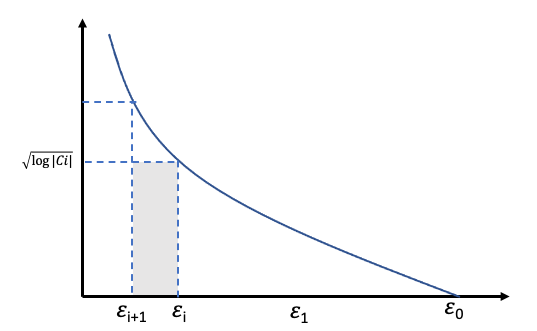
\includegraphics[width=.6\textwidth]{figures/chaining_riemann.png}
        \end{center}
        \caption{We observe that $\log N(\epsilon, \cF, L_2[P_n])$ is monotone decreasing in $\epsilon$. As a result, the right Riemann sum in \eqref{lec9:eqn:dudley_rriemann} will be upper bounded by the integral.}
        \label{lec9:fig:chaining_riemann}
    \end{figure}    

    To complete the proof, observe that $\log N(\epsilon, \cF, L_2[P_n]) = 0$ for all $\epsilon > \epsilon_0$. This allows us to extend the upper limit of the integral given by \eqref{lec9:eqn:dudley_almost} to $\infty$ and yields the desired result:
    \begin{align}
        \Exp\l[\sup_{v \in \cQ} \frac 1 n \inprod{v, \sigma} \r] & \le \frac{12}{\sqrt{n}} \int_{0}^\infty \sqrt{\log N(\epsilon, \cF, L_2[P_n])} d\epsilon
    \end{align}
\end{proof}

\begin{remark}
If $\mathcal{F}$ consists of functions bounded in $[-1,1]$, then, we have that for all $\epsilon > 1, N(\epsilon, \mathcal{F}, L_2[P_n])=1$. To see this choose $\{f\equiv 0\}$, which is a complete cover for $\epsilon>1$. Hence, the limits of integration in \eqref{lec9:eqn:dudley} can be truncated to $[0,1]$:
    
    \begin{equation}
    R_S(\mathcal{F})\leq 12\int_{0}^{1}\sqrt{\frac{\log N(\epsilon, \mathcal{F}, L_2[P_n])}{n}}d\epsilon,
    \end{equation}
    
since $\log N(\epsilon, \mathcal{F}, L_2[P_n])=0$ for $\epsilon >1$.
\end{remark}

\subsec{Covering number regimes for which Dudley's theorem is finite}

Of course, the bound in \eqref{lec9:eqn:dudley} is only useful if the integral on the RHS is finite. Here are some setups where this is the case (we continue to assume that the functions in $\cF$ are bounded in $[-1, 1]$):

\begin{enumerate}
\item If $N(\epsilon, \mathcal{F}, L_2[P_n])\approx (1 / \epsilon)^R$ (ignoring multiplicative and additive constants), then we have $\log N(\epsilon, \mathcal{F}, L_2[P_n]) \approx  R\log (1/\epsilon)$. We can plug this into the RHS of \eqref{lec9:eqn:dudley} to get
        
\begin{equation}
\int_{0}^{1}\sqrt{\frac{\log N(\epsilon, \mathcal{F}, L_2[P_n])}{n}}d\epsilon = \int_{0}^1\sqrt{\frac{R\log(1/\epsilon)}{n}}d\epsilon \approx \sqrt{\frac{R}{n}}.
\end{equation}
            
\item If the covering number has the form $N(\epsilon, \mathcal{F}, L_2[P_n])\approx a^{R/\epsilon}$ for some $a$, then we have $\log N(\epsilon, \mathcal{F}, L_2[P_n]) \approx \frac{R}{\epsilon}\log a$. The bound in \eqref{lec9:eqn:dudley} becomes
        
\begin{align}
\int_0^1\!\!\sqrt{\frac{\log N(\epsilon, \mathcal{F}, L_2[P_n])}{n}}d\epsilon &\approx \int_0^1\!\!\sqrt{\frac{R}{n\epsilon}\log a}\, d\epsilon \\
&= \sqrt{\frac{R}{n}\log a} \int_0^1\!\!\sqrt{\frac{1}{\epsilon}}d\epsilon \\
&= \tilO \l(\sqrt{\frac{R}{n}}\r).
\end{align}
        
\item If the covering number has the form $N(\epsilon, \mathcal{F}, L_2[P_n])\approx a^{R/\epsilon^2}$, then $\log N(\epsilon, \mathcal{F}, L_2[P_n])\approx \frac{R}{\epsilon^2}\log a$. In this case we have:
        
\begin{equation}\int_0^1\sqrt{\frac{\log N(\epsilon, \mathcal{F}, L_2[P_n])}{n}}d\epsilon \approx \sqrt{\frac{R}{n}\log a} \underbrace{\int_0^1\frac{1}{\epsilon}d\epsilon}_{=\infty}=\infty,
\end{equation}

i.e. the bound in \eqref{lec9:eqn:dudley} is vacuous. This is because of the behavior of $\epsilon \mapsto 1/\epsilon^2$ near 0: the function goes to infinity too quickly for us to upper bound its integral. Fortunately, there is an ``improved'' version of Dudley's theorem that is applicable here:
        
\begin{theorem}[Localized Dudley's Theorem]\label{lec9:thm:better-dudley}
If $\cF$ is a function class from $Z$ to $\R$, then for any fixed cutoff $\alpha \geq 0$ we have the bound
\begin{equation}\label{lec9:eqn:better-dudley}
R_S(\mathcal{F})\leq 4\alpha + 12\int_{\alpha}^{\infty}\sqrt{\frac{\log N(\epsilon, \mathcal{F}, L_2[P_n])}{n}}d\epsilon.      
\end{equation}
\end{theorem}
The proof of this theorem is similar to the proof of the original Dudley's theorem, except that the iterative covering procedure is stopped at the threshold $\epsilon = \alpha$ at the cost of the extra $4\alpha$ term above.
        
Theorem \ref{lec9:thm:better-dudley} allows us to avoid the problematic region around $\epsilon=0$ in the integral in \eqref{lec9:eqn:dudley}. If we let $\alpha = 1/\mathsf{poly}(n)$, where $\mathsf{poly}(n)$ denotes some polynomial function of $n$, the bound in \eqref{lec9:eqn:better-dudley} becomes
\begin{align}
R_S(\mathcal{F}) &\leq \frac{1}{\mathsf{poly}(n)} + \frac{\sqrt{R\log a}}{\sqrt{n}}\int_{\alpha}^1\frac{1}{\epsilon}d\epsilon \\
&= \frac{1}{\mathsf{poly}(n)}  + \frac{\sqrt{R\log a}}{\sqrt{n}} \log(1/\alpha) \\
&= \tilO \l(\sqrt{\frac{R}{n}}\r).
\end{align}
\end{enumerate}

In summary, we have that $R_S(\mathcal{F}) \leq \tilO\l(\sqrt{\frac{R}{n}}\r)$ for these three dependencies on $\epsilon$: when $\log N(\epsilon, \mathcal{F}, L_2[P_n]) \approx R\log (1/\epsilon),\ \frac{R}{\epsilon} \log a,\text{ or } \frac{R}{\epsilon^2} \log a$ for some $a$. Note that if the dependence on $\epsilon$ is $1/\epsilon^c$ for $c > 2$, then even the improved Dudley's theorem does not help us. This is because the $\log(1/\alpha)$ term above becomes $\alpha^{1-c/2}$, and when $\alpha = 1/\mathsf{poly}(n)$, this term leads to a bad dependence on $n$.

\subsec{Regimes where we can get covering number bounds}
The previous remarks discuss how strong our bounds on covering number need to be in order to get a useful result. Here we describe some situations in which we know how to obtain these covering number bounds, though we omit the proofs here.

First, consider the following covering number bound for linear models:

\begin{theorem}[\cite{zhang2002}]
Suppose $x^{(1)}, \cdots, x^{(n)} \in \mathbb{R}^d$ are $n$ data points, and $p, q$ satisfies $p^{-1} + q^{-1} = 1$ and $2 \le p \le \infty$. Assume that $||x^{(i)}||_p \le C$ for all $i$. Let:
\begin{align}
    F_q = \{x \to w^T x : ||w||_q \le B\}
\end{align}
and let $\rho = L_2[P_n]$. Then, $\log N(\epsilon, F_q, \rho) \le \l [\frac{B^2c^2}{\epsilon^2}\r ] \log_2 (2d + 1)$. When $p = 2, q = 2$, we further obtain that:
\begin{align}
    \log N(\epsilon, F_2, \rho) \le \l [\frac{B^2c^2}{\epsilon^2} \r ] \log_2 (2 \min (n, d ) + 1)
\end{align}
\end{theorem}
\begin{remark}
Using the covering number bound derived above, it is also possible to show that the Rademacher complexity of this class of linear models is bounded by
\begin{align}
    R_s(F_q) &\le \tilO{\left( \frac{BC}{\sqrt{n}} \right)}
\end{align} 
\end{remark}
For multivariate linear functions, let $\norm{M^T}_{2,1}$ denote the sum of the $\ell_2$ norms of the $n$ rows of $M$ where $M = (M_1, \cdots, M_n) \in \mathbb{R}^{m \times n}$. 
\begin{theorem}
Let $\cF = \{x \to Wx : W \in \mathbb{R}^{m \times d}, ||W^T||_{2, 1} \le B\}$ and let $C = \sqrt{\frac{1}{n} \sum_{i = 1}^n ||x^{(i)}||_2^2}$. Then, 
\begin{equation}
\log N(\epsilon, F, L_2(P_n)) \le \l [\frac{c^2B^2}{\epsilon^2} \r ] \log (2dm).
\end{equation}
\end{theorem}

Covering numbers also interact nicely with composition by Lipschitz functions. The following result is the analog of Talagrand's lemma for covering numbers.
\begin{lemma} Suppose $\phi$ is $\kappa$-Lipschitz, and $\rho = L_2[P_n]$. Then,
    \begin{align}
        \log N(\epsilon, \phi \circ \cF, \rho) \le \log N(\epsilon / \kappa, \cF, \rho) \label{lec9:eqn:covering-num-lipschitz}
    \end{align}
\end{lemma}
\begin{proof}
Let $\cC$ denote an $\epsilon/\kappa$-cover for $\cF$. Then $\phi \circ \cC$ is an $\epsilon$-cover of $\phi \circ \cF$.
\begin{align}
\rho(\phi \circ f', \phi \circ f) &= \sqrt{\frac{1}{n} \sum (\phi(f'(z_i)) - \phi(f(z_i)))^2} \\ 
&\le \sqrt{\frac{1}{n} \cdot \kappa^2 \sum(f'(z_i) - f(z_i))^2}\\
&\le \kappa \cdot \frac{\epsilon}{\kappa} = \epsilon
\end{align}
\end{proof}

Using these results, we can obtain a bound on the Rademacher complexity of a dense neural network. Consider a deep network
\begin{equation}
f(x) = W_r\sigma(W_{r-1}\sigma(\cdots \sigma(W_1x)\ldots),
\end{equation}

where $W_i$ are layer-wise weights and $\sigma$ is an activation function which is 1-Lipschitz. For this setup we have the following Rademacher complexity bound:
\begin{equation}
R_S (\cF) \leq \underbrace{\l(\prod_{i=1}^r\|W_i\|_{\textup{op}} \r)}_{\text{relatively large}} \cdot \underbrace{\l( \sum_{i=1}^r\frac{\|W_i^\top\|^{2/3}_{2,1}}{\|W_i\|_{\textup{op}}^{2/3}}\r)^{3/2}}_{\text{relatively small}}.
\end{equation}
        
Here $\|W\|_{\textup{op}}$ is the operator norm (or spectral norm) of $W$, and $\|W_i^\top\|_{2,1}$ denotes the sum of the $l_2$ norms of the rows of $W_i$. The second term is relatively small as it is a sum of matrix norms, and so the bound is dominated by the first term, which is a product of matrix norms. This first term comes from composition of Lipschitz functions as in \eqref{lec9:eqn:covering-num-lipschitz} above, since the Lipschitz constant of a linear operator is its spectral norm. The full details are presented in \cite{bartlett2017}.


\sec{VC dimension and its limitations}
We will focus on classification and will be working within the framework of supervised learning stated in Chapter \ref{chap:supervised}. The labels belong to the output space $\mathcal{Y} = \{-1, 1\}$, each classifier is a function $h:\mathcal{X}\to\R$ for all $h \in \cH$, and the prediction is the sign of the output, i.e. $\hat{y} = \sgn(h(x))$. We will look at zero-one loss, i.e. $\err((x,y), h) = \mathbbm{1}(\sgn(h(x))\neq y)$. Note that we can re-express the loss function as
\begin{equation}
\err((x,y), h) = \frac{1-\sgn(h(x))y}{2}.
\end{equation}

The first approach is to reason directly about the Rademacher complexity of $\err$ loss, i.e. considering the family of functions $\cF = \left\{ z = (x, y) \mapsto \err((x, y), h) : h \in \cH \right\}$. Define $Q$ to be the set of all possible outputs on our dataset: $Q=\left\{\left(\sgn\left(h\left(x^{(1)}\right)\right), \dots, \sgn \left(h\left(x^{(n)}\right)\right)\right)\mid  h \in \cH \right\}$. Then, using our earlier remark about viewing the empirical Rademacher complexity as an inner product between $v\in Q$ and $\sigma$, we have
\begin{align}
R_S(\cF) &= \Exp_{\sigma_1,\dots, \sigma_n} \l[ \sup_{f\in \cF} \frac{1}{n} \sum^n_{i=1} \sigma_i \frac{1-\sgn(h(x^{(i)}))y_i}{2} \r] \\
&= \Exp_{\sigma_1,\dots, \sigma_n} \l[ \sup_{f\in \cF} \frac{1}{n} \sum^n_{i=1} \sigma_i \frac{\sgn(h(x^{(i)}))}{2} \r] \\
&= \frac{1}{2}\Exp_{\sigma_1,\dots, \sigma_n} \l[ \sup_{v\in Q} \frac{1}{n} \langle \sigma, v\rangle \r].
\end{align}

Notice that the supremum is now over $Q$ instead of $\cF$. If $n$ is sufficiently large, then it is typically the case that $|Q|>|\cF|$. To see why this is the case, note that each function $f$ corresponds to a single element in $Q$. However, as $n$ increases, $|Q|$ increases as well. For any particular $v\in Q$, notice that $\langle v, \sigma\rangle$ is a sum of bounded random variables, so we can use Hoeffding's inequality to obtain
\begin{equation}
\Pr\left[\frac{1}{n}\langle\sigma, v\rangle\geq t\right] \leq \exp (-n t^2 / 2).
\end{equation}
Taking the union bound over $v\in Q$, we see that 
\begin{equation}
\Pr\left[\exists v\in Q \text{ such that } \frac{1}{n}\langle\sigma, v\rangle \geq t\right] \leq |Q| \exp (-nt^2 / 2).
\end{equation}
Thus, with probability at least $1-\delta$, it is true that $\sup _{v \in Q} \frac{1}{n}\langle v, \sigma \rangle \leq \sqrt{\frac{2(\log|Q| + \log (2/\delta))}{n}}$. Similarly, we can show that $\Exp \left[ \sup _{v \in Q} \frac{1}{n}\langle v, \sigma \rangle \right] \leq O\l(\sqrt{\frac{\log|Q| + \log (2/\delta)}{n}}\r)$ holds.

The key point to notice here is that the upper bound on $R_S(\cF)$ depends on $\log |Q|$. \textit{VC dimension} is one way that we deal with bounding the size of $Q$ We will not delve into the details of this approach (for those interested, see Section 3.11 of \cite{percynotes}). VC dimension, however, has a number of limitations. For one, we will always end up with a bound that depends somehow on the dimension. For linear models, we obtain a bound $\log |Q| \lesssim d \log n$, corresponding to a bound on Rademacher complexity that looks like
\begin{equation}
R_S(\cF) \leq \tilO \left( \sqrt{\frac{d}{n}} \right),
\end{equation}
so we still have a $\sqrt{d}$ term. This will not be a good bound for high-dimensional models. For general models, we will arrive a bound of the form 
\begin{equation}
R_S(\cF) \leq \tilO \left( \sqrt{\frac{\text{\# of parameters}}{n}} \right).
\end{equation}
This upper bound only depends on the number of parameters in our model, and does not take into the account the scale and norm of the parameters. Additionally, this doesn't work with kernel methods since the explicit parameterization is possibly infinite-dimensional, and therefore this upper bound becomes useless.

These limitations motivation the use of margin theory, which does take into account the norm of parameters and provides a theoretical basis for regularization techniques such as $L_1$ and $L_2$ regularization.
	
	\chapter{Rademacher Complexity Bounds for Concrete Models and Losses}\label{chap:gen-bounds}
	% reset section counter
%\setcounter{section}{0}

%\metadata{lecture ID}{Your names}{date}
\metadata{6}{Daniel Do}{February 1st, 2021}

In this chapter, we will instantiate Rademacher complexity for two important hypothesis classes: linear models and two-layer neural networks. In the process, we will develop margin theory and use it to bound the generalization gap for binary classifiers.

\sec{Margin theory for classification problems}

\subsec{Intuition}
Assume that we are in the same setting as in the previous section. A fundamental problem we face in this setting is that we do not have a continuous loss: everything is discrete in the output space. We need to find a way to reason about the scale of the output. An example of this is logistic regression: the logistic regression model outputs a probability, and while we compare it to the outcome (0 or 1), how close it is to the true output gives us a measure of how confident we are in the prediction.

Figure \ref{lec6:fig:margin} gives similar intuition for linear classifiers. Intuitively, the black line is a "better" decision boundary than the red line because the minimum distance from any point to the black boundary is greater than the minimum distance from any point to the red line. In the next section, we will formalize this intuition by proving that the larger this margin is, the smaller the bound on generalization gap is.

\begin{figure}[ht!]
    \begin{center}
  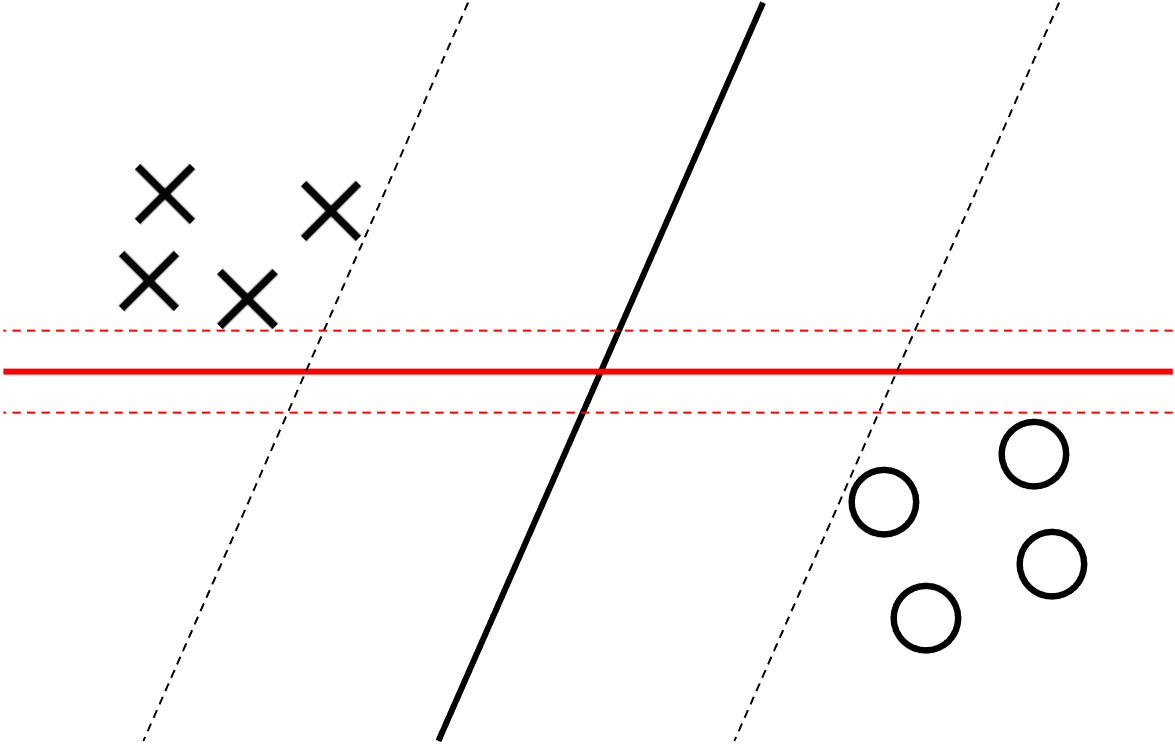
\includegraphics[width=0.5\textwidth]{figures/margin.png}
  \end{center}
  \caption{The red and black lines are two decision boundaries. The X's are positive examples and the O's are negative examples. The black line has a larger margin than the red line, and is intuitively a better classifier.}
  \label{lec6:fig:margin}
\end{figure}

\subsec{Formalizing margin theory}
First, assume that the dataset $\cD = ((x\sp{1}, y\sp{1}), \dots, (x\sp{n}, y\sp{n}))$ is \textit{completely separable}. In other words, there exists some $h_\theta\in\cH$ such that $y^{(i)} = \sgn(h_\theta(x^{(i)}))$ holds for all $( x^{(i)},y^{(i)})\in \cD$. This is not a necessary condition for our final bound but will make the derivation cleaner.

\begin{definition}[(Unnormalized) Margin]
Fix the hypothesis $h_\theta$. The \textit{(unnormalized) margin} for example $(x, y)$ is defined as $\margin(x) = yh_\theta(x)$. Margin is only defined on examples where $\sgn(h_\theta(x)) = y$. (Note that $\margin(x)\geq 0$ because of our assumption of complete separability.)
\end{definition}

\begin{definition}[Minimum margin] Given a dataset $\cD = ((x\sp{1}, y\sp{1}), \dots, (x\sp{n}, y\sp{n}))$, the \textit{minimum margin} over the dataset is defined as $\gamma_{\min} \triangleq \min_{i\in\{1,\dots,|\cD|\}} y^{(i)}h_\theta(x^{(i)})$.
\end{definition}

Our final bound will have the form (generalization gap)$\leq f(\text{margin},\text{parameter norm})$. This is very generic since there are many different bounds we could derive based on what margin we use. For this current setting we are using $\gamma_{\min}$, which is the minimum margin, but in other settings could use $\gamma_{\text{average}}$, which is the average margin of each point in the dataset.

We will begin by introducing the idea of a \textit{surrogate loss}, a loss function which approximates zero-one loss but takes the scale of the margin into account. The \textit{margin loss} (also known as \textit{ramp loss}) is defined as 
\begin{equation}
    \ell_\gamma(t) = \begin{cases} 
      0 & t\geq \gamma \\
      1 & t\leq 0 \\
      1-t/\gamma & 0\leq t\leq \gamma
   \end{cases}
\end{equation}

\begin{figure}[ht!]
    \begin{center}
  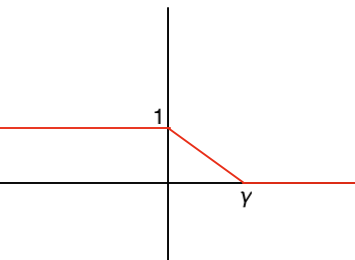
\includegraphics[width=0.5\textwidth]{figures/margin_loss.png}
  \end{center}
  \caption{Plotted margin loss.}
  \label{lec6:fig:marginloss}
\end{figure}

It is plotted in Figure \ref{lec6:fig:marginloss}. For convenience, define $\ell_\gamma((x,y), h) \triangleq \ell_\gamma(yh(x))$. We can view $\ell_\gamma$ as a continuous version of $\err$ while being more sensitive to the scale of the margin on $[0,\gamma]$. Notice that $\err$ is always less than or equal to the $\ell_\gamma$ when $\gamma\geq 0$, i.e.
\begin{equation}
    \err((x,y), h) = \ind{yh(x) < 0}\leq \ell_\gamma(yh(x)) =\ell_\gamma ((x,y), h)
\end{equation}
holds for all $(x,y)\sim P$. Taking the expectation over $(x,y)$ on both sides of this inequality, we see that
\begin{equation}
    L(h) = \Exp_{(x,y)\sim P} \left[ \err((x,y), h) \right] \leq \Exp_{(x,y)\sim P} \left[ \ell_\gamma ((x,y), h) \right].
\end{equation}

Therefore, the population loss is bounded by the expectation of the margin loss, and so it is sufficient to bound the expectation of the margin loss in order to bound the population loss.

Define the population and empirical version of the margin loss:
\begin{equation}
L_\gamma(h) = \Exp_{(x,y)\sim P}\l[ \ell_\gamma((x,y), h)\r], \quad \hat{L}_\gamma(h) = \sum_{i=1}^n\l [\ell_\gamma((x^{(i)},y^{(i)}), h)\r].
\end{equation}

By Corollary \ref{lec6:cor:ggap-rsbound}, we see that with probability at least $1-\delta$ that
\begin{equation}
L_\gamma(h) - \hat{L}_\gamma(h)\leq 2R_S(\cF) + 3\sqrt{\frac{\log (2/\delta)}{2n}},
\end{equation}
where $\cF = \{(x,y)\mapsto \ell_\gamma((x,y), h)\mid h\in\cH\}$. Note that if we set $\gamma\leq \gamma_{\min}$, then $\hat{L}_{\gamma}(h) = 0$. This follows because by definition of $\gamma_{\min}$, $y^{(i)}h(x^{(i)})\geq \gamma_{\min}$ for any $(x^{(i)}, y^{(i)})\in \cD$. As a result, $\ell_\gamma((x^{(i)}, y^{(i)}), h) = \ell_\gamma(y^{(i)}h(x^{(i)})) = 0$ holds. Therefore, it suffices to bound $R_S(\cF)$.

We will now use \textit{Talagrand's lemma} to bound $R_S(\cF)$ in terms of $R_S(\cH)$ to remove any dependence on the loss function from the upper bound. 
 
\begin{lemma}[Talagrand's lemma] \label{lec6:lem:talagrand_lemma}
Let $\phi:\R\to\R$ be a $\kappa$-Lipschitz function. Then \begin{equation}
    R_S(\phi\circ \cH)\leq \kappa R_S(\cH),
\end{equation} 
where $\phi\circ\cH = \{z\mapsto \phi(h(z))\mid h\in\cH\}$.
\end{lemma}

We can use Talagrand's lemma directly with $\phi(t) = \ell_\gamma(t)$, which is $\frac{1}{\gamma}$-Lipschitz. We can express $\cF$ as $\cF=\ell_\gamma\circ\cH'$ where $\cH' = \{(x,y)\to yh(x)\mid h\in\cH\}$. Applying Talagrand's lemma, we see that

\begin{align}
R_S(\cF) &\leq \frac{1}{\gamma}R_S(\cH') \\
&= \frac{1}{\gamma}\Exp_{\sigma_1,\dots, \sigma_n} \l[ \sup_{h\in \cH} \frac{1}{n} \sum^n_{i=1} \sigma_i y^{(i)}h(x^{(i)}) \r] \\
&= \frac{1}{\gamma}\Exp_{\sigma_1,\dots, \sigma_n} \l[ \sup_{h\in \cH} \frac{1}{n} \sum^n_{i=1} \sigma_i h(x^{(i)})  \r] \\
&= \frac{1}{\gamma}R_S(\cH).
\end{align}

Putting this all together, we have shown that for $\gamma = \gamma_{\min}$,
\begin{align}
\Err(h) \leq L_\gamma(h) &\leq 0 + O \left( \frac{R_S(\cH)}{\gamma} \right) + \tilO \left( \sqrt{\frac{\log (2 / \delta)}{2n}} \right) \\
&= O \left( \frac{R_S(\cH)}{\min_i y\sp{i} h(x\sp{i}) } \right) + \tilO \left( \sqrt{\frac{\log (2 / \delta)}{2n}} \right).
\end{align}

In other words, for training data of the form $S = \{(x\sp{i},y\sp{i})\}_{i=1}^n \subset \mathbb{R}^d \times \{-1,1\}$, a hypothesis class~$\mathcal{H}$ and 0-1 loss, we can derive a bound of the form
\begin{equation}\label{lec7:eqn:generalization_loss}
    \text{generalization loss} \leq \frac{2R_S(\mathcal{H})}{\gamma_{\mathrm{min}}} + \text{low-order term},
\end{equation}
where $\gamma_\mathrm{min}$ is the minimum margin achievable on~$S$ over those hypotheses in $\cH$ that separate the data, and $R_S(\cH)$ is the empirical Rademacher complexity of $\cH$. Such bounds state that simpler models will generalize better beyond the training data, particularly for data that is strongly separable.

\begin{remark} \label{lec7:rmk:union_bound_margin}
Note there is a subtlety here. If we think of the dataset as random, it follows that $\gamma_{\min}$ is a random variable. Consequently, the $\gamma$ we choose to define the hypothesis class is random, which is not a valid choice when thinking about Rademacher complexity! Technically we cannot apply Talagrand's lemma with a random $\kappa$ (which we took to be $1/\gamma$). Also, when we used concentration inequalities, we implicitly assume that the $\ell_\gamma((x\sp{i}, y\sp{i}), h)$ are independent of each other. That is not the case if $\gamma$ is dependent on the data.

We sketch out how one might address this issue below. The main idea is to do another union bound over $\gamma$. Choose a family $\Gamma = \left\{ 2^k: k \in [-B, B] \right\}$ for some $B$. Then, for every fixed $\gamma \in \Gamma$, with probability greater than $1 - \delta$,
\begin{align}
\Err(h) \leq \hatL_\gamma (h) + O \left( \frac{R_S(\cH)}{\gamma} \right) + \tilO \left( \sqrt{\frac{\log \frac{1}{\delta}}{n}} \right).
\end{align}
Taking a union bound over all $\gamma \in \Gamma$, it further holds that for all $\gamma \in (0, B)$, 
\begin{align}
    \Err(h) \leq \hatL_\gamma (h) + O \left( \frac{R_S(\cH)}{\gamma} \right) + \tilO \left( \sqrt{\frac{\log \frac{1}{\delta}}{n}}\right) + \tilO \left ( \sqrt{\frac{\log B}{n}} \right ). \label{lec7:eqn:unionboundmargin}
\end{align}
Last, choose the largest $\gamma \in \Gamma$ such that $\gamma \leq \gamma_{\min}$. Then, for this value of $\gamma$, our desired bound directly follows from the bound in \eqref{lec7:eqn:unionboundmargin}. Namely, we have that $\hatL_{\gamma} (h) = 0$ and $O \left( \frac{R_S(\cH)}{\gamma} \right) = O \left( \frac{R_S(\cH)}{\gamma_{\min}} \right)$. The additional term, $\tilO\left ( \sqrt{\frac{\log B}{n} }\right )$, is the price exacted by the uniform convergence argument required to correct the heuristic bound given in \eqref{lec7:eqn:generalization_loss}.

\end{remark}
	% reset section counter
%\setcounter{section}{0}

%\metadata{lecture ID}{Your names}{date}
\metadata{7}{Spencer M.~Richards and Thomas Lew}{Feb.~3rd, 2021}

\sec{Linear models}\label{lec7:sec:lin_models}

\subsec{Linear models with weights bounded in \texorpdfstring{$\ell_2$}{L2} norm}
We begin with the Rademacher complexity of linear models using weights with bounded $\ell_2$ norm.

\begin{theorem}\label{lec7:thm:l2-thm}
    Let $\mathcal{H} = \{x \mapsto \inprod{w,x} \mid w \in \R^d, \Norm{w}_2 \le B\}$ for some constant $B > 0$. Moreover, assume $\Exp_{x \sim P}\sbr{\Norm{x}_2^2} \leq C^2$, where $P$ is some distribution and $C > 0$ is a constant. Then
    \begin{align}
        R_S(\mathcal{H}) &\le \frac{B}{n} \sqrt{\sum_{i=1}^n \Norm{x\sp{i}}_2^2},  \label{lec7:eqn:linear-sample}
        \intertext{and}
        R_n(\mathcal{H}) &\le \frac{BC}{\sqrt{n}}.  \label{lec7:eqn:linear}
    \end{align}
\end{theorem}

Generally speaking, there are two methods with which we can bound the Rademacher complexity of a model. The first method, which we used in Chapter \ref{chap:uc}, consists of discretizing the space of possible outputs from our hypothesis class, then using a union bound or covering number argument to bound the Rademacher complexity of the model. While this method is powerful and generally applicable, it yields bounds that depend on the logarithm of the cardinality of this discretized output space, which in turn depends on the number of data points~$n$. In the proof below, we will instead use a more elegant, albeit limited technique which does not rely on discretization of the output space.

\begin{proof}
We start with the proof of \eqref{lec7:eqn:linear-sample}. By definition,
\begin{align}
    R_S(\mathcal{H}) 
    &= \Exp_\sigma\sbr{ \sup_{\Norm{w}_2 \le B} \frac{1}{n} \sum_{i=1}^n\sigma_i \inprod{w,x\sp{i}} }
    \\&= \frac{1}{n} \Exp_\sigma\sbr{ \sup_{\Norm{w}_2 \le B} \inprod{w,\sum_{i=1}^n\sigma_i x\sp{i}} }
    \\&= \frac{B}{n} \Exp_\sigma\sbr{ \Norm{\sum_{i=1}^n \sigma_i  x\sp{i}}_2 }
        &&\text{($\textstyle\sup_{\Norm{w}_2 \le B} \langle w,v\rangle =B\Norm{v}_2$)}
    \\&\leq \frac{B}{n} \sqrt{ \Exp_\sigma\sbr{\Norm{ \sum_{i=1}^n \sigma_i x\sp{i} }_2^2} }
        &&\text{(Jensen's ineq. for $\alpha \mapsto \alpha^2$)} 
    \\&= \frac{B}{n} \sqrt{ \Exp_\sigma \sbr{\sum_{i=1}^n \rbr{\sigma_i^2 \Norm{x\sp{i}}_2^2 + \inprod{\sigma_ix\sp{i},\sum_{j \ne i}^n \sigma_j x\sp{j}} }} }
    \\&= \frac{B}{n} \sqrt{\sum_{i=1}^n \Norm{x\sp{i}}_2^2}.
        &&\text{($\sigma_i$ indep. and $\Exp[\sigma_i]=0$)}
\end{align}
This completes the proof of \eqref{lec7:eqn:linear-sample} for the empirical Rademacher complexity. The bound on the average Rademacher complexity in \eqref{lec7:eqn:linear} follows from taking the expectation of both sides to get
\begin{equation}
    R_n(\mathcal{H}) = \Exp\sbr{ R_S(\mathcal{H}) }
    = \frac{B}{n} \Exp\sbr{ \sqrt{\sum_{i=1}^n \Norm{x\sp{i}}_2^2} }
    \le \frac{B}{n} \sqrt{ \sum_{i=1}^n \Exp\sbr{\Norm{x\sp{i}}_2^2} }
    \le \frac{BC}{\sqrt{n}},
\end{equation}
where the first inequality is another application of Jensen's inequality, and the second follows from the assumption $\Exp_{x \sim P}\sbr{\Norm{x}_2^2} \leq C^2$.

\end{proof}

We observe that both the empirical and average Rademacher complexities scale with the upper $\ell_2$-norm bound $\Norm{w}_2 \le B$ on the parameters~$w$, which motivates regularizing the model. However, smaller weights in the model may reduce the margin $\gamma_\mathrm{min}$, which in turn hurts generalization according to \eqref{lec7:eqn:generalization_loss}.

\begin{remark}
Note that if we scale the data by some multiplicative factor, the bound on empirical Rademacher complexity $R_S(\cH)$ will scale accordingly. However, at the same time, we expect the margin to scale by the same multiplicative factor, so the bound on the generalization gap in \eqref{lec7:eqn:generalization_loss} does not change. This lines up with our intuition that the bound should not depend on the scaling of the data.
\end{remark}

\subsec{Linear models with weights bounded in \texorpdfstring{$\ell_1$}{L1} norm}
Now, we consider linear models again, except we restrict the $\ell_1$-norm of the parameters and assume an $\ell_\infty$-norm bound on the data.

\begin{theorem}\label{lec7:thm:l1-thm}
    Let $\mathcal{H} = \cbr{x \mapsto \inprod{w,x} \mid w \in \R^d, \Norm{w}_1 \le B}$ for some constant $B > 0$. Moreover, assume $\Norm{x\sp{i}}_\infty \leq C$ for some constant $C > 0$ and all points in $S = \{x\sp{i}\}_{i=1}^n \subset \R^d$. Then
    \begin{equation}
        R_S(\mathcal{H}) \leq BC\sqrt{\frac{2\log(2d)}{n}}.
    \end{equation}
\end{theorem}

To prove the theorem, we will need Massart's lemma, which provides a bound for the Rademacher complexity of a finite hypothesis class.

    \begin{lemma}[Massart's lemma]
        Suppose $\mathcal{Q} \subset \R^n$ is finite and contained in the $\ell_2$-norm ball of radius $M\sqrt{n}$ for some constant $M > 0$, i.e.,
        \begin{equation}
            \mathcal{Q} \subset \{v \in \R^n \mid \Norm{v}_2 \leq M\sqrt{n} \}.
        \end{equation}
        Then, for Rademacher variables $\sigma = (\sigma_1,\sigma_2,\dots,\sigma_n) \in \R^n$,
        \begin{equation}
            \Exp_\sigma \left[ \sup_{v\in \mathcal{Q}} \frac{1}{n}\inprod{\sigma,v} \right] \leq M\sqrt{\frac{2\log|\mathcal{Q}|}{n}}.
        \end{equation}
        As a corollary, if $\mathcal{F}$ is a set of real-valued functions satisfying
        \begin{equation}
            \sup_{f\in\mathcal{F}} \frac{1}{n}\sum_{i=1}^n f(z\sp{i})^2 \leq M^2,
        \end{equation}
        over some data $S = \{z\sp{i}\}_{i=1}^n$, then
        \begin{align}
            R_S(\mathcal{F}) \leq M\sqrt{\frac{2\log|\mathcal{F}|}{n}}, \quad\text{and}\quad
            R_n(\mathcal{F}) \leq M\sqrt{\frac{2\log|\mathcal{F}|}{n}}.
        \end{align}
    \end{lemma}

We will not prove Massart's lemma in detail. The intuition is to use concentration inequalities to bound $\frac{1}{n}\inprod{\sigma, v}$ for fixed $v$, then to use a union bound over the elements $v \in \mathcal{Q}$.

We will now prove Theorem \ref{lec7:thm:l1-thm}:

\begin{proof}[Proof of Theorem \ref{lec7:thm:l1-thm}]
    By definition,
    \begin{align}
        R_S(\mathcal{H}) &= \Exp_\sigma\sbr{ \sup_{\Norm{w}_1 \le B} \frac{1}{n} \sum_{i=1}^n\sigma_i \inprod{w,x\sp{i}} } \\
        &= \frac{1}{n} \Exp_\sigma\sbr{ \sup_{\Norm{w}_1\le B} \inprod{w,\sum_{i=1}^n\sigma_i x\sp{i}} } \\
        &= \frac{B}{n} \Exp_\sigma\sbr{ \Norm{\sum_{i=1}^n \sigma_i  x\sp{i}}_\infty  },
    \end{align}
    
    where the last equality is because $\sup_{\Norm{w}_1 \leq B}\inprod{w,v} = B\Norm{v}_\infty$, i.e., the $\ell_\infty$-norm is the dual of the $\ell_1$-norm, which is a consequence of H\"older's inequality. However, the $\ell_\infty$-norm is difficult to simplify further. Instead, we use the fact that $\sup_{\Norm{w}_1 \leq 1} \inprod{w,v}$ for any $v \in \R^d$ is always attained at one of the vertices $\mathcal{W} = \bigcup_{i=1}^d \{-e_i,e_i\}$, where $e_i \in \R^d$ is the $i$-th coordinate unit vector. Defining the restricted hypothesis class $\bar{\mathcal{H}} = \{x \mapsto \inprod{w,x} \mid w \in \mathcal{W}\} \subset \mathcal{H}$, this yields
    \begin{align}
        R_S(\mathcal{H}) &= \frac{1}{n} \Exp_\sigma\sbr{ \sup_{\Norm{w}_1 \le B} \inprod{w,\sum_{i=1}^n\sigma_i x\sp{i}} } \\
        &= \frac{B}{n} \Exp_\sigma\sbr{ \max_{w\in\mathcal{W}} \inprod{w,\sum_{i=1}^n\sigma_i x\sp{i}} } \\
        &= BR_S(\bar{\mathcal{H}}).
    \end{align}
    
    In particular, the model class $\bar{\mathcal{H}}$ is bounded and finite with cardinality $|\bar{\mathcal{H}}| = 2d$. This suggests using Massart's lemma to complete the proof. To do so, we need to confirm that $\mathcal{\bar{H}}$ is bounded with respect to the $\ell_2$-metric. Indeed, since the inner product of $x\sp{i}$ with a coordinate vector $e_j$ just selects the $j$-th coordinate of $x\sp{i}$, for any $w \in \mathcal{W}$ we have
    \begin{equation}
        \frac{1}{n}\sum_{i=1}^n \inprod{w,x\sp{i}}^2 \leq \frac{1}{n}\sum_{i=1}^n \Norm{x\sp{i}}^2_\infty \leq \frac{1}{n}\sum_{i=1}^n C^2 = C^2,
    \end{equation}
    where the last inequality uses the assumption $\Norm{x_i}_\infty \leq C$. So $\bar{\mathcal{H}}$ is bounded in the $\ell_2$-metric and finite, thus by Massart's Lemma we have
    \begin{equation}
        R_S(\mathcal{H}) = B R_S(\bar{\mathcal{H}}) \leq BC\sqrt{\frac{2\log|\bar{\mathcal{H}}|}{n}} = BC\sqrt{\frac{2\log(2d)}{n}},
    \end{equation}
    which completes the proof.
\end{proof}

\subsec{Comparing the bounds for different \texorpdfstring{$\cH$}{H}}

First, we note that for this hypothesis class of linear models, it is possible to obtain an upper bound proportional to $\sqrt{d/n}$ using the VC~dimension, which grows quickly with the data dimension~$d$. Our bound is better since it does not have as strong of a dependence on~$d$, and accounts for the norms of our model parameters and the data.

In the two subsections above, we considered two different hypothesis classes of linear models, each restricting different norms. In both cases, the bound on the average Rademacher complexity depended on the product of the norm bound on the parameters $w$ and the norm bound on each data point $x$. To determine which choice of hypothesis class is better, consider the bounds
    \begin{equation*}
        \Norm{w}_2\Norm{x}_2 \quad\text{vs.}\quad \Norm{w}_1\Norm{x}_\infty
    \end{equation*}
    and see how they compare in different settings. We consider 3 settings here:
    
    \begin{itemize}
    \item Suppose $w$ and $x$ are random variables with $w_i$ and $x_i$ close to the set of values $\{-1,1\}$. Then we have
    \begin{equation*}
        \sqrt{d}\cdot \sqrt{d} \quad\text{vs.}\quad d\cdot 1.
    \end{equation*}
    In this case, there is no difference in using either linear hypothesis class.
    
    \item If we additionally suppose $w$ is sparse with at most $k$ non-zero entries, then we have
    \begin{equation*}
        \sqrt{k}\cdot\sqrt{d} \quad\text{vs.}\quad k\cdot 1.
    \end{equation*}
    So for $d \gg k$, we have $\sqrt{kd} \gg k$ and thus $\ell_1$-norm regularization leads to a better complexity bound when $w$ is suspected to be sparse. Indeed, $\sqrt{d}\Norm{x}_\infty \approx \Norm{x}_2$ when the entries of $x$ are somewhat uniformly distributed, and so in the sparse case we have
    \begin{equation}
        \Norm{w}_2\Norm{x}_2 \geq \sqrt{d}\Norm{w}_2\Norm{x}_\infty \geq \Norm{w}_1\Norm{x}_\infty. 
    \end{equation}
    
    \item On the other hand, if $w$ is dense in the sense that $\Norm{w}_2\approx {\sqrt{d}}\Norm{w}_1$ (i.e., if all entries in $w$ are close to each other in magnitude), then
    \begin{equation}
        \Norm{w}_2\Norm{x}_2 \leq \frac{1}{\sqrt{d}}\Norm{w}_1 \cdot \sqrt{d} \Norm{x}_\infty \leq \Norm{w}_1\Norm{x}_\infty.
    \end{equation}
    In this case, it makes sense to regularize the $\ell_2$-norm instead.
    \end{itemize}
    
    In practice, other multiplicative factors enter the generalization bound, so regularizing both the $\ell_1$- and $\ell_2$-norms of the model parameters $w$ is preferable.

    Continuing with this rough style of analysis, for the hypothesis class with restricted $\ell_2$-norm, we can write the bound on the generalization gap in \eqref{lec7:eqn:generalization_loss} as
    \begin{equation}
        \text{generalization loss} \lesssim \frac{\Norm{w}_2\Norm{x}_2}{\sqrt{n}\gamma_{\mathrm{min}}} + \text{low-order term}.
    \end{equation}
    The presence of $\Norm{w}_2/\gamma_{\mathrm{min}}$ motivates both the minimum norm and the maximum margin formulations of the Support Vector Machine (SVM) problem as good methods to improve generalization performance of binary classifiers.

%*****************************************************************************
\sec{Two-layer neural networks}
We now compute a bound for the Rademacher complexity of two-layer neural networks.  Throughout this section, we use the following notation:
\begin{itemize}
    \item $\theta = (w, U)$ are the parameters of the model with $w \in \R^m$ and $U \in \R^{m \times d}$, where $m$ denotes the number of hidden units. We use $u_i\in\R^d$ to denote the $i$-th row of $U$ (written as a column vector).
    \item $\phi(z) = \max(z, 0)$ is the ReLU activation function applied element-wise.
    \item $f_\theta(x) = \inprod{w,\phi(Ux)} = w^\top \phi(Ux)$ is the model.
    \item $\{ (x\sp{i}, y\sp{i}) \}_{i=1}^n$ is the training set, with $x\sp{i}\in\R^d$ and $y\sp{i}\in\R$.
\end{itemize}
We start with a somewhat weak bound which introduces the technical tools we need to derive tighter bounds subsequently.

\begin{theorem}\label{lec7:thm:thm_3}
    For some constants $B_w > 0$ and $B_u > 0$, let
    \begin{equation}
        \mathcal{H} = \cbr{ f_\theta \mid \Norm{w}_2 \leq B_w,\ \Norm{u_i}_2 \leq B_u,\ \forall i \in \{1,2,\dots,m\} }, \label{lec7:eqn:thm_3}
    \end{equation}
    and suppose $\Exp\sbr{\Norm{x}_2^2} \leq C^2$. Then
    \begin{align}
        R_n(\mathcal{H}) \le 2 B_w B_u C\sqrt{\frac{m}{n}}.
    \end{align}
\end{theorem}

This bound is not ideal as it depends on the number of neurons~$m$. Empirically, it has been found that the generalization error does \emph{not} increase monotonically with~$m$. As more neurons are added to the model, thereby giving it more expressive power, studies have shown that generalization is improved \cite{belkin2019}. This contradicts the bound above, which states that more neurons leads to worse generalization. We also note that the theorem can be generalized straightforwardly to the setting where the $w$ and $U$ are jointly constrained in the sense that we set $\mathcal{H} = \cbr{ f_\theta \mid \Norm{w}_2\cdot \left(\max_i\Norm{u_i}_2\right) \leq B}$ and obtain the generalization bound $        R_n(\mathcal{H}) \le 2 B C\sqrt{\frac{m}{n}}.$ However, the $\sqrt{m}$ dependency still exists under this formulation of $\cH$. 
Nevertheless, we now derive this bound.

\begin{proof}
    By definition,
    \begin{align}
        R_S(\mathcal{H}) 
        &= \Exp_\sigma\sbr{ \sup_\theta \frac{1}{n} \sum_{i=1}^n \sigma_i \inprod{w,\phi(Ux\sp{i})} }
        \\&= \frac{1}{n} \Exp_\sigma\sbr{ \sup_{U : \Norm{u_j}_2 \leq B_u} \sup_{\Norm{w}_2 \leq B_w} \inprod{w,\sum_{i=1}^n \sigma_i \phi(Ux\sp{i})} }
        \\&= \frac{B_w}{n}\Exp_\sigma\sbr{ \sup_{U : \Norm{u_j}_2 \leq B_u} \Norm{ \sum_{i=1}^n \sigma_i \phi(Ux\sp{i})}_2 }
            &&\text{($\textstyle\sup_{\Norm{w}_2\leq B}\inprod{w,v} = B\Norm{v}_2$)}
        \\&\leq \frac{B_w\sqrt{m}}{n}\Exp_\sigma\sbr{ \sup_{U : \Norm{u_j}_2 \leq B_u} \Norm{ \sum_{i=1}^n \sigma_i \phi(Ux\sp{i})}_\infty }
            &&\text{($\Norm{v}_2 \leq \sqrt{m}\Norm{v}_\infty$)}
        \\&= \frac{B_w\sqrt{m}}{n}\Exp_\sigma\sbr{ \sup_{U : \Norm{u_j}_2 \leq B_u} \max_{1\leq j\leq m} \abs{ \sum_{i=1}^n \sigma_i \phi(u_j^\top x\sp{i})} } 
        \\&= \frac{B_w\sqrt{m}}{n}\Exp_\sigma\sbr{ \sup_{\Norm{u}_2 \leq B_u} \abs{ \sum_{i=1}^n \sigma_i \phi(u^\top x\sp{i})} }
        \\&\leq \frac{2B_w\sqrt{m}}{n}\Exp_\sigma\sbr{ \sup_{\Norm{u}_2 \leq B_u} \sum_{i=1}^n \sigma_i \phi(u^\top x\sp{i}) }
            &&\text{(by Lemma \ref{lec8:lemma:absfortwo})} \label{lec7:eqn:nn-proof1}
        \\&\leq \frac{2B_w\sqrt{m}}{n}\Exp_\sigma\sbr{ \sup_{\Norm{u}_2 \leq B_u} \sum_{i=1}^n \sigma_i u^\top x\sp{i} }, \label{lec7:eqn:nn-proof2}
    \end{align}
    where the last inequality follows by applying the contraction lemma (Talagrand's lemma) and observing that the ReLU function is $1$-Lipschitz. (Observe that the expectation in \eqref{lec7:eqn:nn-proof1} is the Rademacher complexity for $\{ x \mapsto \phi(u^\top x) \mid \Norm{u}_2 \leq B_u \}$: this is the family that we are applying the contraction lemma to.)
    
    We now observe that the expectation in \eqref{lec7:eqn:nn-proof2} is the Rademacher complexity of the family of linear models $\{x \mapsto \inprod{u,x} \mid \Norm{u}_2\leq B_u\}$. Thus, applying Theorem~\ref{lec7:thm:l1-thm} yields
    \begin{equation}
        R_S(\mathcal{H}) \leq \frac{2B_w\sqrt{m}}{n}B_u\sqrt{\sum_{i=1}^n \Norm{x\sp{i}}_2^2}.
    \end{equation}
    
    Taking the expectation of both sides and using similar steps to those in the proof of Theorem~\ref{lec7:thm:l1-thm} gives us
    \begin{align}
        R_n(\mathcal{H})  &= \Exp\left[ R_S(\mathcal{H})\right] \\
        &\leq \frac{2B_wB_u\sqrt{m}}{n} \Exp\sbr{\sqrt{\sum_{i=1}^n \Norm{x\sp{i}}_2^2}} \\
        &\leq \frac{2B_wB_u\sqrt{m}}{n} C\sqrt{n} \\
        &= 2 B_w B_u C\sqrt{\frac{m}{n}},
    \end{align}
    which completes the proof.
    
\end{proof}

This upper bound is undesirable since it grows with the number of neurons $m$, contradicting empirical observations of the generalization error decreasing with $m$.

%*****************************************************************************

\subsec{Refined bounds}
\newcommand{\boundsforcomp}{B}
Next, we look at a finer bound that results from defining a new complexity measure. A recurring theme in subsequent proofs will be the functional invariance of two-layer neural networks under a class of rescaling transformations. The key ingredient will be the \textit{positive homogeneity} of the ReLU function, i.e.
\begin{equation}
\alpha \phi(x) = \phi(\alpha x) \qquad \forall \alpha > 0.
\end{equation}
This implies that for any $\lambda_i > 0$ ($i = 1, \dots, m$), the transformation $\theta = \{(w_i, u_i)\}_{1 \leq i \leq m} \mapsto \theta' = \{(\lambda_i w_i,  u_i / \lambda_i )\}_{1 \leq i \leq m}$ has no net effect on the neural network's functionality (i.e. $f_{\theta} = f_{\theta'}$) since 
\begin{equation}
w_i\cdot \phi \left(u_i^\top x\sp i \right) = (\lambda_i w_i) \cdot \phi\l(\l( \frac{u_i}{\lambda_i}\r)^\top x\sp i\r).   
\end{equation}
In light of this, we devise a new complexity measure $C(\theta)$ that is also invariant under such transformations and use it to prove a better bound for the Rademacher complexity. This positive homogeneity property is absent in the complexity measure used in the hypothesis class \eqref{lec7:eqn:thm_3} of Theorem \ref{lec7:thm:thm_3}.

\begin{theorem}\label{lec8:thm:thm-improved-nn-rc}
$\operatorname{Let} C(\theta)=\sum_{j=1}^{m}\left|w_{j}\right|\left\|u_{j}\right\|_{2},$ and for some constant $\boundsforcomp>0$ consider the hypothesis class
\begin{equation}
\mathcal{H}=\left\{f_{\theta} \mid C(\theta) \leq \boundsforcomp\right\}. \label{eqn:H}
\end{equation}
If $\left\|x\sp{i}\right\|_{2} \leq C$ for all $i \in\{1, \ldots, n\},$ then
\begin{equation}
R_{S}(\mathcal{H}) \leq \frac{2 \boundsforcomp C}{\sqrt{n}}.
\end{equation}
\end{theorem}

\begin{remark}
	Compared to Theorem~\ref{lec7:thm:thm_3}, this bound does not explicitly depend on the number of neurons $m$. Thus, it is possible to use more neurons and still maintain a tight bound if the value of the new complexity measure $C(\theta)$ is reasonable. In contrast, the bound of Theorem \ref{lec7:thm:thm_3} explicitly grows with the total number of neurons. In fact, Theorem~\ref{lec8:thm:thm-improved-nn-rc} is strictly stronger than Theorem~\ref{lec7:thm:thm_3} as elaborated below. Note that 
	\begin{align}
		\sum |w_j|\|u_j\|_2 &\le \left(\sum |w_j|^2\right)^{1/2} \left(\sum\|u_j\|_2^2\right)^{1/2} \tag{by Cauchy-Schwarz inequality} \\
		& \le \|w\|_2 \cdot \sqrt{m} \cdot \max_{j}\|u_j\|_2
	\end{align}
	Therefore, if we consider $\cH^1 = \{f_\theta \mid \sum |w_j|\|u_j\|_2\le B'\}$ and $\cH^2 = \{f_\theta \mid \|w\|_2 \cdot \sqrt{m} \cdot \max_{j}\|u_j\|_2 \le B'\}$, then either Theorem~\ref{lec8:thm:thm-improved-nn-rc} on $\cH^1$ or Theorem~\ref{lec7:thm:thm_3} on $\cH^2$ gives the same generalization bound $O(B'/\sqrt{n})$, but $\cH^1 \supset \cH^2$. 
	
	Moreover, Theorem~\ref{lec8:thm:thm-improved-nn-rc} is stronger as we have more neurons---this is because the hypothesis class $\cH$ as defined in~\eqref{eqn:H} is bigger as $m$ increases. Because of this, it's possible to obtain a generalization guarantee that decreases as $m$ increases, as shown in Section~\ref{sec:gen-bounds:decreasing-in-m}. 
	
%	For example, consider solving the constrained problem
%	\begin{equation}
%	\rho_m = \min_\theta C(\theta) 
%	\quad \text{such that}\quad 
%	\text{$f_\theta$ fits the data  $\{(x\sp{i}, y\sp{i})\}_{i=1}^n$.}
%	\end{equation}
%	In this case, $\rho_m$ monotonically decreases as the number of neurons $m$ increases. Indeed, models with more parameters necessarily include models with a lower number of parameters and thus those of lower complexity.  As a result, it is possible to obtain lower complexity models by increasing the number of parameters $m$.
\end{remark}

\begin{proof}[Proof of Theorem~\ref{lec8:thm:thm-improved-nn-rc}]
Due to the positive homogeneity of the ReLU function $\phi$, it will be useful to define the $\ell_2$-normalized weight vector $\bar{u}_j \defeq u_j / \norm{u_j}_2$ so that $\phi\left(u_j^\top x\right) = \norm{u_j}_2 \cdot \phi(\bar{u}_j^\top x)$. The empirical Rademacher complexity satisfies
\allowdisplaybreaks
\al{
R_S(\cH) &= \frac{1}{n}\Exp_{\sigma}\left[ \sup_{\theta} \sum_{i=1}^n \sigma_i f_{\theta}\left(x\sp{i}\right) \right] \\
&= \frac{1}{n}\Exp_{\sigma}\left[ \sup_{\theta} \sum_{i=1}^n \sigma_i \left[\sum_{j=1}^m w_j \phi\left(u_j ^ T x\sp{i}\right) \right] \right] &&\text{(by dfn of $f_\theta$)} \\
&=  \frac{1}{n}\Exp_{\sigma}\left[ \sup_{\theta} \sum_{i=1}^n \sigma_i \left[\sum_{j=1}^m w_j \norm{u_j}_2  \phi\left(\bar{u}_j ^ T x\sp{i}\right) \right] \right]  
    && \text{(by positive homogeneity of $\phi$)}\\
&= \frac{1}{n}\Exp_{\sigma}\left[ \sup_{\theta}  \sum_{j=1}^m w_j \norm{u_j}_2 \left[ \sum_{i=1}^n \sigma_i  \phi\left(\bar{u}_j ^ T x\sp{i}\right) \right] \right] \\ 
&\leq \frac{1}{n}\Exp_{\sigma}\left[ \sup_{\theta}  \sum_{j=1}^m |w_j| \norm{u_j}_2 \max_{k \in [n]}\left| \sum_{i=1}^n \sigma_i  \phi\left(\bar{u}_k ^ T x\sp{i}\right) \right| \right] && \l(\because \sum_j \alpha_j \beta_j \leq \sum_j |\alpha_j| \max_{k} |\beta_k|\r) \\ 
&\leq \frac{\boundsforcomp}{n} \Exp_{\sigma}\sbr{ \sup_{\theta = (w, U)} \max_{k \in [n]} \left| \sum_{i=1}^n \sigma_i  \phi\left(\bar{u}_k ^ T x\sp{i}\right) \right| } && \text{($\because C(\theta) \leq \boundsforcomp$)} \\
&=  \frac{\boundsforcomp}{n} \Exp_{\sigma}\sbr{ \sup_{\bar{u}: \norm{\bar{u}}_2 = 1} \left| \sum_{i=1}^n \sigma_i  \phi\left(\bar{u} ^ T x\sp{i}\right) \right| } \\
&\le \frac{\boundsforcomp}{n} \Exp_{\sigma}\sbr{ \sup_{\bar{u}: \norm{\bar{u}}_2 \le 1} \left| \sum_{i=1}^n \sigma_i  \phi\left(\bar{u} ^ T x\sp{i}\right) \right| } \\
&\le \frac{2\boundsforcomp}{n}  \Exp_{\sigma}\sbr{ \sup_{\bar{u}: \norm{\bar{u}}_2 \le 1} \sum_{i=1}^n \sigma_i  \phi\left(\bar{u} ^ T x\sp{i}\right) } && \text{(see Lemma \ref{lec8:lemma:absfortwo})} \\
&= 2\boundsforcomp R_S(\cH '),
}
where $\cH' = \l\{x \mapsto \phi(\bar{u}^\top x) :  \bar{u} \in \mathbb{R}^d, \norm{\bar{u}}_2 \leq 1 \r\}$. By Talagrand's lemma, since $\phi$ is $1$-Lipschitz, $R_S(\cH') \leq R_S(\cH'')$ where  $\cH'' = \l\{x \mapsto \bar{u}^\top x :  \bar{u} \in \mathbb{R}^d, \norm{\bar{u}}_2 \leq 1 \r\}$ is a linear hypothesis space. Using $R_S(\cH'') \leq \frac{C}{\sqrt{n}}$ by Theorem \ref{lec7:thm:l2-thm} then concludes the proof.

\end{proof}

We complete the proof by deriving the Lemma \ref{lec8:lemma:absfortwo} used in the second-to-last inequality. Notably, the lemma's assumption holds in the current context, since
\al{
\sup_{\theta} \langle \sigma, f_{\theta}(x) \rangle = \sup_{\bar{u}: \norm{\bar{u}}_2 \leq 1} 
\sum_{i=1}^n \sigma_i \phi \l(\bar{u}^\top x\sp i \r)  \geq 0.
}
since one can take $\bar{u} = 0$ for any $\sigma = (\sigma_1, \dots, \sigma_n)$.

\begin{lemma}\label{lec8:lemma:absfortwo}
Let $\sigma = (\sigma_1, ..., \sigma_n)$ and $f_{\theta}(x) = \l(f_{\theta}\l(x\sp{1}\r), ...,  f_{\theta}\l(x\sp{n} \r)\r)$. Suppose that for any $\sigma \in \{\pm 1\}^n$, $\sup_{\theta} \langle \sigma, f_{\theta}(x) \rangle \geq 0$. Then, 
\begin{equation}
\mathbb{E}_{\sigma}\l[ \sup_{\theta}  \l | \langle \sigma, f_{\theta}(x) \rangle \r|  \r] \leq 2 \mathbb{E}_{\sigma}\l[ \sup_{\theta}  \langle \sigma, f_{\theta}(x) \rangle   \r].
\end{equation}
\end{lemma}

\begin{proof}
Letting $\phi$ be the ReLU function, the lemma's assumption implies that $\sup_{\theta} \phi\left(\langle \sigma, f_{\theta}(x) \rangle\right) = \sup_{\theta}\langle \sigma, f_{\theta}(x) \rangle$ for any $\sigma \in \{\pm 1\}^n$. Observing that $|z| = \phi(z) + \phi(-z)$, 
\begin{align}
\sup_{\theta} \abs{\inprod{ \sigma, f_{\theta}(x) }}%
&= \sup_{\theta} \left[ \phi \l(\inprod{ \sigma, f_{\theta}(x) } \r) + \phi \l(\inprod{-\sigma, f_{\theta}(x) } \r)\right] \\
&\le \sup_{\theta}  \phi \l(\inprod{ \sigma, f_{\theta}(x) } \r) +  \sup_{\theta}  \phi \l(\inprod{-\sigma, f_{\theta}(x) } \r)  \\
&= \sup_{\theta} \inprod{ \sigma, f_{\theta}(x) } +  \sup_{\theta}  \inprod{-\sigma, f_{\theta}(x) }. 
\end{align}
Taking the expectation over $\sigma$ (and noting that $\sigma \overset d = -\sigma$), we get the desired conclusion.
\end{proof}



\sec{More implications and discussions on two-layer neural nets}
In this section, we discuss practical implications of the refined neural network bound. 

\subsec{Connection to \texorpdfstring{$\ell_2$}{L2} regularization}\label{sec:gen-bounds:impliciation}

Recall that margin theory yields
\begin{equation}
\text{for all } \theta, \quad \Err(\theta) \leq \frac{2R_S(\cH)}{\gammamin} + \tilO\l(\sqrt{\frac{\log \l( 2 / \delta \r)}{n}}\r), \label{lec8:eqn:margin-bound}
\end{equation}
with probability at least $1 -\delta$. Thus, Theorem \ref{lec8:thm:thm-improved-nn-rc} motivates us to minimize $\frac{R_S(\cH)}{\gammamin}$ by regularizing $C(\theta)$. Concretely, this can be formulated as the optimization problem 
\al{
\text{minimize} & \qquad C(\theta) = \sum_{j=1}^m |w_j|\cdot \norm{u_j}_2 \nonumber \tag{I} \label{lec8:eqn:opt1} \\ 
\text{subject to} & \qquad \gammamin(\theta)\ge 1, \nonumber
}
or equivalently,
\al{
\text{maximize} & \qquad \gammamin(\theta) \nonumber \tag{II} \label{lec8:eqn:opt2} \\ 
\text{subject to} & \qquad C(\theta)\le 1. \nonumber
}

At first glance, the above seems orthogonal to techniques used in practice. However, it turns out that the optimal neural network from \eqref{lec8:eqn:opt1} is functionally equivalent to that of the new problem:
\al{
\text{minimize} & \qquad C_{\ell_2}(\theta) = \frac{1}{2}\sum_{j=1}^m |w_j|^2 + \frac{1}{2}\sum_{j=1}^m \norm{u_j}_2^2 \nonumber \tag{I*} \label{lec8:eqn:opt1star} \\ 
\text{subject to} & \qquad \gammamin(\theta)\ge 1. \nonumber
}
This is a simple consequence of the positive homogeneity of $\phi$. For any scaling factor $\lambda=(\lambda_1, \dots, \lambda_m)\in \R_+^m$, the rescaled neural network $\theta_\lambda \defeq \{(\lambda_i w_i, u_i/\lambda_i)\}$ has the same functionality as the original neural network $\theta = \{w_i, u_i \}$ (i.e. it achieves the same $\gammamin$). Thus, 
\al{
\min_{\theta} C_{\ell_2}(\theta) &= \min_{\theta} \min_{\lambda} \rbr{ \frac{1}{2}\sum_{j=1}^m \lambda_j^2 |w_j|^2 + \frac{1}{2}\sum_{j=1}^m \lambda_j^{-2}\norm{u_j}_2^2 }\\
&= \min_{\theta}  \sum_{j=1}^m |w_j|\cdot \norm{u_j}_2 \\
&= \min_{\theta}  C(\theta)
}
where we have used the equality case of the AM-GM inequality, attainable by $\lambda_j^* = \sqrt{\frac{\norm{u_j}_2}{|w_j|}}$, in the second step. This equality case also shows that $\theta^* = \{(w_i, u_i ) \}$ is the optimal solution of \eqref{lec8:eqn:opt1} if and only if $\hat{\theta}^* = \theta_{\lambda^*}$ is the optimal solution of \eqref{lec8:eqn:opt1star}---proving that $\hat{\theta}^*$ and $\theta^*$ are functionally equivalent since they only differ by a positive scale factor. 

This connects our $C(\theta)$ regularization to $\ell_2$-norm penalties that are more prevalent in practice. In retrospect, we see this equivalence is essentially due to the positive homogeneity of the neural network which ``homogenizes'' any inhomogeneous objective such as $C_{\ell_2}$. Hence, we can just deal with $C(\theta)$ which is transparently homogeneous.

\subsec{Generalization bounds that are decreasing in \texorpdfstring{$m$}{m}} \label{sec:gen-bounds:decreasing-in-m}

Next, we show that the generalization bound given by Theorem \ref{lec8:thm:thm-improved-nn-rc} does not deteriorate with the network width (number of neurons) $m$, which is consistent with experimental results. To this end, the perspective of \eqref{lec8:eqn:opt2} enables us to isolate all dependencies of $m$ in $\gammamin$. Letting $\widehat \theta_m$ denote the minimizer of program \eqref{lec8:eqn:opt2} with width $m$ and defining optimal value $\gamma_m^* = \gammamin\l(\widehat \theta_m\r)$, we can rewrite the margin bound \eqref{lec8:eqn:margin-bound} as 
\begin{equation}
L(\widehat \theta_m) \le \frac{4C}{\sqrt{n}} \cdot \frac{1}{\gamma_m^*} + \text{(lower-order terms)},
\end{equation}
where all dependencies on $m$ are now contained in $\gamma_m^*$. Hence, to show that this bound does not worsen as $m$ grows, we just have to show that $\gamma_m^*$ is non-decreasing in $m$. This is intuitively the case since a neural network of width $m+1$ contains one of width $m$ under the same complexity constraints. The following theorem formalizes this hunch:

\begin{theorem}
Let $\gamma_m^*$ be the minimum margin obtained by solving \eqref{lec8:eqn:opt2} with a two-layer neural network of width $m$. Then $\gamma_m^* \leq \gamma_{m+j}^*$ for all positive integers $j$.
\end{theorem}

\begin{proof}
Suppose $\theta = \{(w_i, u_i)\}_{1 \leq i \leq m}$ is a two-layer neural network of width $m$ satisfying $C(\theta)\le 1$. Then we may construct a neural network $\widetilde \theta = \{(\tilde w_i, \tilde u_i)\}_{1 \leq i \leq m+1}$ of width $m+1$ by simply taking
\al{
(\widetilde w_i, \widetilde u_i) = \begin{cases}
(w_i, u_i) & i\le m, \\
(0,0) & \text{otherwise.}
\end{cases}
}
$\widetilde \theta$ is functionally equivalent to $\theta$ and $C(\widetilde \theta) = C(\theta) \le 1$. This means maximizing $\gammamin$ over $\{C(\widetilde \theta): \widetilde \theta\text{ of width }m+1\}$ should give no lower of a value than the maximum of $\gammamin$ over $\{C(\theta): \theta\text{ of width }m\}$.
\end{proof}

\subsec{Equivalence to an \texorpdfstring{$\ell_1$}{L1}-SVM in \texorpdfstring{$m \to \infty$}{m -> inf} limit}

Since $\gamma_m^*$ is non-decreasing in $m$, the quantity 
\begin{equation}
\gamma_\infty ^* = \lim_{m\to \infty } \gamma_m^*
\end{equation}
is well-defined. The next interesting fact is that in this $m \to \infty$ limit, $\gamma_{\infty}^*$ of the two-layer neural network is equivalent to the minimum margin of an $\ell_1$-SVM. As a brief digression, we recap the formulation of $\ell_p$-SVMs and discuss the importance of $\ell_1$-SVMs in particular.

Since a collection of data points with binary class labels may not be a priori separable, a \textit{kernel model} first transforms an input $x$ to $\varphi(x)$ where $\varphi: \mathbb{R}^d \to \mathcal{G}$ is known as the \textit{feature map}. The model then seeks a separating hyperplane in this new (extremely high-dimensional) feature space $\mathcal{G}$, parameterized by a vector $\mu$ pointing from the origin to the hyperplane. The prediction of the model on an input $x$ is then a decision score that quantifies $\varphi(x)$'s displacement with respect to the hyperplane:
\begin{equation}
g_{\mu, \varphi}(x) \defeq \l\langle \mu, \varphi(x) \r\rangle.
\end{equation}
Motivated by margin theory, it is desirable to seek the maximum-margin hyperplane under a constraint on $\mu$ to guarantee the generalizability of the model. In particular, a kernel model with an $\ell_p$-constraint seeks to solve the following program:
\al{
\text{maximize} & \qquad \gamma_{min} \coloneqq \min_{i \in [n]} y\sp{i}\langle \mu, \varphi(x\sp{i}) \rangle \\ 
\text{subject to} & \qquad \norm{\mu}_p \le 1. \nonumber
}
Observe that both the prediction and optimization of the feature model only rely on inner products in $\mathcal{G}$. The ingenuity of the SVM is to choose maps $\varphi$ such that $K(x, x') = \l\langle \varphi(x), \varphi(x') \r\rangle$ can be directly computed in terms of $x$ and $x'$ in the original space $\mathbb{R}^d$, thereby circumventing the need to perform expensive inner products in the large space $\mathcal{G}$. Remarkably, this ``kernel trick'' enables us to even operate in an implicit, infinite-dimensional $\mathcal{G}$. 

The case of $p=1$ is particularly useful in practice as $\ell_1$-regularization generally produces sparse feature weights (the constrained parameter space is a polyhedron and the optimum tends to lie at one of its vertices). Hence, $\ell_1$-regularization is an important feature selection method when one expects only a few dimensions of $\cG$ to be significant. Unfortunately, the $\ell_1$-SVM is not kernelizable due to the kernel trick relying on $\ell_2$-geometry, and is hence infeasible to implement. However, our next theorem shows that a two-layer neural network can approximate a particular $\ell_1$-SVM in the $m \to \infty$ limit (and in fact, for finite $m$). For the sake of simplicity, we sacrifice rigor in defining the space $\mathcal{G}$ and convey the main ideas.

\begin{theorem}\label{lec8:thm:thm8.5}
Define the feature map $\phirelu: \mathbb{R}^d \to \mathcal{G}$ such that $x$ is mapped to $\phi(u^\top x)$ for all vectors $u$ on the $d-1$-dimensional sphere $\mathcal{S}^{d-1}$. Informally, 
$$\phirelu(x) \defeq \begin{bmatrix} \vdots \\ \phi(u^\top x) \\ \vdots \end{bmatrix}_{u\in S^{d-1}}$$
is an ``infinite-dimensional vector'' that contains an entry $\phi(u^\top x)$ for each vector $u \in \mathcal{S}^{d-1}$, and we let $\phirelu(x)[u]$ denote the ``$u$''-th entry of this vector. Noting that $\mathcal{G}$ is the space of functions which can be indexed by $u \in S^{d-1}$, the inner product structure on $\mathcal{G}$ is defined by $\langle f, g \rangle = \int_{S^{d-1}} f[u]g[u] du$.

Under this set-up, we have
\begin{equation}
\gamma_{\infty}^* = \gamma_{\ell_1}^*,
\end{equation}
where $\gamma_{\ell_1}^*$ is the minimum margin of the optimized $\ell_1$-SVM with $\varphi = \phirelu$.
\end{theorem}

\begin{proof}

We will only prove the $\gamma_{\infty}^* \leq \gamma_{\ell_1}^*$ direction. (The $\gamma_{\infty}^* \geq \gamma_{\ell_1}^*$ direction requires substantial functional analysis.)

Suppose $\gamma_\infty^*$ is obtained by network weights $(w_1,w_2, \cdots), (u_1, u_2, \cdots)$ where $w_i\in \R, u_i\in \R^d$ (there is a slight subtlety here to be rectified later). Define renormalized versions of $\{w_i\}$ and $\{u_i\}$:
\begin{equation}
\widetilde w_i \defeq w_i\cdot \norm{u_i}_2, \qquad \overline u_i \defeq \frac {u_i} {\norm{u_i}_2}.   
\end{equation}
Note that $\{(\widetilde w_i, \overline u_i)\}$ has the same functionality (and also the same complexity measure $C(\theta)$, margin, etc.) as that of $\{(w_i,u_i)\}$, but now $\overline u_i$ has unit $\ell_2$-norm (i.e. $\bar{u}_i \in \mathcal{S}^{d-1}$). Thus, $\phi(\overline u_i ^\top x)$ can be treated as a feature in $\cG$ and we can construct an equivalent $\ell_1$-SVM (denoted by $\mu$) such that $\widetilde w_i$ is the coefficient of $\mu$ associated with that feature. Since $\widetilde w_i$ must only be ``turned on" at $\overline u_i $, we have 
\al{
\mu[u] = \sum_{i \in \mathcal{S}^{d-1}} \tilde{w}_i \delta(u - \overline u_i),
}
where $ \delta(u)$ is the Dirac-delta function. Given this $\mu$, we can check that the SVM's prediction is
\al{
g_{\mu, \phirelu}(x) &= \int_{S^{d-1}} \mu[u] \phirelu(x)[u] du \\
&= \int_{S^{d-1}}   \sum_{i \in \mathcal{S}^{d-1}} \tilde{w}_i \delta(u - \overline u_i) \phi\left(\overline u ^\top x\right) du \\
&= \sum_{i \in \mathcal{S}^{d-1}}  \tilde{w}_i \phi\left(\overline u_i ^\top x\right) ,
}
which is identical to the output $f_{\{(\widetilde w_i, \overline u_i)\}}(x)$ of the neural network. Furthermore, 
\al{
\norm{\mu}_1 =  \sum_{i=1}^{\infty} |\widetilde w_i| = \sum_{i=1}^{\infty} |w_i|\cdot \norm{u_i}_2 \leq 1,
}
where the last equality holds because $\{(\widetilde w_i, \overline u_i)\}$ satisfies the constraints of \eqref{lec8:eqn:opt2}. This shows that our constructed $\mu$ satisfies the $\ell_1$-SVM constraint. Thus, $\gamma_{\infty}^* \leq \gamma_{\ell_1}^*$ since the functional behavior of the optimal neural network is contained in the search range of the SVM.

\end{proof}

\begin{remark}
How well does a finite-dimensional neural network approximate the infinite-dimensional $\ell_1$ network? Proposition B.11 of \cite{wei2020regularization} shows that you only need $n+1$ neurons. Another way to say this is that $\{\gamma_m\}$ stabilizes once $m=n+1$:
\begin{equation}
\gamma_1^* \le \gamma_2^* \le \dots \le \gamma_{n+1}^* = \gamma_\infty^*.
\end{equation}
The main idea of the proof is that if we have a neural net $\theta$ with $(n+2)$ neurons, then we can always pick a simplification $\theta'$ with $(n+1)$ neurons such that $\theta,\theta'$ agree on all $n$ datapoints.

As an aside, this result also resolves the issue in our partial proof. A priori, $\gamma_{\infty}^*$ may not necessarily be attained by a set of weights $\{(\widetilde w_i, \overline u_i)\}$, but the above shows that it is achievable with just $n+1$ non-zero indices.

\end{remark}

	
	\chapter{Theoretical Mysteries in Deep Learning}
	% reset section counter
\setcounter{section}{0}

%\metadata{lecture ID}{Your names}{date}
\metadata{9}{Rafael Rafailov and Aidan Perreault}{Feb 10th, 2021}

We now turn to a high-level overview of deep learning theory. To begin, we outline a framework for classical machine learning theory, then discuss how the situation is different from deep learning theory.

\sec{Framework for classical machine learning theory}
At the risk of oversimplification, we can divide classical machine learning theory into three parts:

\begin{enumerate}
\item {\bf Approximation theory} attempts to answer whether there is any choice of parameters $\theta$ that achieves low population error. In other words, is the choice of hypothesis class good enough to approximate the ground truth function? Using notation from earlier in this course, the goal is to upper bound $L(\theta^*) = \min_{\theta \in \Theta} L(\theta).$
    
\item {\bf Statistical generalization} focuses on bounding the excess risk $L(\hat{\theta}) - L(\theta^*)$. In Chapter \ref{chap:uc} we obtained the following bound:
    
\begin{equation}
L(\hat{\theta})-L(\theta^*)\leq \underbrace{L(\hat{\theta})-\hat{L}(\hat{\theta})}_{\text{generalization error}} + |L(\theta^*)-\hat{L}(\theta^*)|.
\end{equation}
    
The first term here is the generalization error, which usually has an upper bound of the form $R(\theta)/\sqrt{n}$, where $R(\theta)$ is some complexity measure.\footnote{In earlier chapters, we defined the complexity of a hypothesis class, not of a specific parameter value. To reconcile these two approaches, think of $R$ as a measure of complexity (such as a norm) that we can then use to define a hypothesis class $\Theta$, i.e.~$\Theta = \{\theta' : R(\theta') \le R(\theta)\}$.} This is a demonstration of \textit{Occam's Razor}: the principle that simple (low-complexity) explanations generalize better. 
    
This statistical approach allows us to define a regularized loss  $\hat{L}_{\textup{reg}}(\theta)=\hat{L}(\theta)+\lambda R(\theta)$. Minimizing this loss gives us a solution $\hat{\theta}_\lambda$ which simultaneously has low training error and low complexity, which lets us bound both the training error and the generalization error. To summarize, in the classical setting, we can prove statements of the form
    
\begin{equation}\label{lec9:eqn:classical-guarantee}
\text{If }\hat{\theta}_\lambda \text{ minimizes } \hat{L}_{\textup{reg}},\text{ then } L(\hat{\theta}_\lambda) - L(\theta^*) \text{ is small.}
\end{equation}

\item {\bf Optimization} considers how to obtain the minimizer $\hat\theta$ or $\hat{\theta}_\lambda$ computationally. This usually involves convex optimization: if $\hat{L}$ or $\hat{L}_{\textup{reg}}$ is convex, then we have a polynomial-time algorithm to find the global minimum.
\end{enumerate}

While there are many tradeoffs to consider between these three components (for example, we may be able to find a loss function for which optimization is easy, but generalization becomes worse), it is still possible to study each area individually, then combine all three to get a result.

\sec{Deep learning theory and its differences}
The situation is more complex for deep learning theory. Two prominent differences are (a) the models are non-linear and the objective functions are non-convex, and (b) in deep learning, researchers have observed in many cases that more parameters typically help improve the performance, and many state-of-the-art models have much more parameters than the number of training data. (b) is often referred as to ``over-parameterization". \tnoteimp{add the figure overparameterization.png in the figure folder and add some caption (feel free to trim the figure and move the citation info to the caption)}

Let us consider the difference in each of the three components described for classical machine learning theory. 

\begin{enumerate} 
\item {\bf Approximation theory:} Large neural net models are considered to be very expressive. That is, both the population loss $L(\theta^*)$ and the finite sample loss $\hat{L}(\hat\theta)$ can be made small. In fact, neural networks are \textit{universal approximators}; see for example \cite{hornik1991}. This can be a somewhat misleading statement as the definition of universal approximator allows for the size of the network to be impracticably large, but morally it seems to hold true in practice anyway.
        
This expressivity is possible because neural networks are usually highly \textit{over-parametrized}: they have many more parameters than samples. It is possible to prove that in this regime, the network can ``memorize'' the entire dataset and achieve approximately zero training error.
    
\item {\bf Statistical generalization:} Relatively weak regularization is used in practice. In many cases only weak $\ell_2$ regularization is used, i.e.
\begin{equation}
\widehat{L}_{\textup{reg}}(\theta)=\hat{L}(\theta)+\lambda\|\theta\|_2^2.
\end{equation}
    
The first interesting fact is that this regularized loss does not have a unique (approximate) global minimizer. This is due to overparametrization: there are so many degrees of freedom that there are many approximate global minimizers with approximately the same $\ell_2$ norm.
    
However, it turns out that these global minimizers are not equally good: many models which achieve zero training error may have very bad test error. Take, for example, using stochastic gradient descent (SGD) to learn a model to classify the dataset CIFAR-10. Consider two instantiations of this: one starting with a large learning rate and slowly decreasing it, and one with a small learning rate throughout. Even though both instantiations result in approximately zero training error, the former leads to much better test performance. \tnoteimp{add deep-learning-implicit-reg.png in the figure folder. perhaps can also include ``bad global min'' as a demonstration}

Therefore, the goal in deep learning theory is not just to find an arbitrary global minimum: we need to find the right global minimum. This contrasts sharply with \eqref{lec9:eqn:classical-guarantee} from the classical setting, where achieving a global minimum leads to good guarantees on generalization error. This means that \eqref{lec9:eqn:classical-guarantee} is simply not powerful enough to deal with deep learning, because it cannot distinguish between $\theta$'s with good test error and bad test error.

\item {\bf Optimization:} The discussion above means that optimization plays a significant role in generalization for deep learning. Different training algorithms have different ``implicit biases'', causing them to converge to different global minimizers. Understanding the implicit biases of algorithms is thus a central goal of deep learning theory. It is impossible to design a good optimization algorithm without also considering its impact on generalization. In fact, many algorithms for non-convex optimization have been proposed that work well for minimizing training loss, but because their implicit bias is different, they lead to worse test performance and are therefore not too useful.
    
Often these implicit biases can be interpreted as encouraging $\hat\theta$ to have low complexity in some sense. The deep learning analog of  \eqref{lec9:eqn:classical-guarantee} is that ``low complexity solutions generalize''. This means that we end up doing more work on the optimization front in order to understand the implicit bias of our algorithm, and then proving generalization bounds works similarly to the classical setting once we understand how our optimizer finds a low-complexity solution.
    
\end{enumerate}

To explain the success of deep learning, we will cover three tasks in the next two chapters:

\begin{enumerate}
    \item Prove that our optimization algorithm converges to an approximate global minimum, even though the objective function is non-convex. Our results here will mostly be for simplified models (e.g. linearized neural nets). (We will also show later that this can be accomplished separately from the other tasks using a special optimization setup (the ``NTK approach"). However, the generalization of this approach can be poor.)
    
    \item Show that the solution $\hat{\theta}$ has low complexity $R(\hat{\theta})\leq C$. We can only answer this question for some special cases of models (e.g. logistic regression, matrix factorization) and optimizers (e.g. gradient descent, label noise in SGD, dropout, learning rate).
    
    \item Show that for all $\theta$ such that $R(\theta)\leq C$ with $\hat{L}(\theta)\approx 0$, we have $L(\theta)$ is small. That is, we show that low-complexity solutions to the empirical risk problem generalize well. We will be working with more fine-grained complexity measures, and several of the tools we used in classical machine learning can still apply.
\end{enumerate}
	
	\chapter{Nonconvex Optimization}
	% reset section counter
\setcounter{section}{0}

%\metadata{lecture ID}{Your names}{date}
\metadata{10}{Kevin Han and Han Wu}{Feb 17th, 2021}

In the previous chapter, we outlined conceptual topics in deep learning theory and how the situation was different from classical machine learning theory. In particular, we described \textit{approximation theory}, \textit{statistical generalization} and \textit{optimization}. In this chapter, we will focus on optimization theory in deep learning. We will introduce some basics about optimization (Section~\ref{sec:optim_convergence}), discuss how we can make the notion ``all local minima are global minima'' rigorous, and walk through two examples where this is the case (Section~\ref{sec:two_optim_examples}). Finally, we introduce the neural tangent kernel approach which allows us to characterize of the loss of general neural networks near a specific initialization (or under specific parameterization).

\sec{Optimization landscape} \label{sec:optim_intro}

The big question that we have in mind is the following: many existing optimizers are designed for optimizing convex functions. \textbf{Why do they still work well empirically for non-convex functions?} We note that it is not true that these optimizers always work well with non-convex functions: there are still some very hard cases that give trouble (e.g. very deep feed-forward networks are still hard to fit because of issues like vanishing and exploding gradients). One possible reason is that the non-convex functions that we are minimizing in deep learning usually have some nice properties: see Figure \ref{lec10:fig:optimization} for an illustration.

\begin{figure}[ht!]
    \centering
    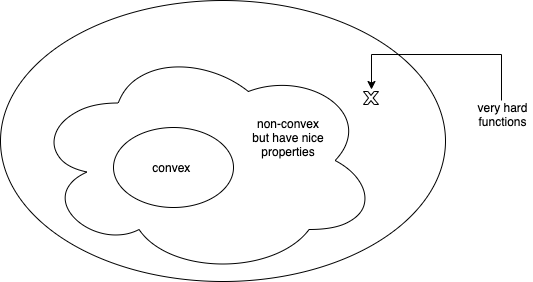
\includegraphics[scale = 0.5]{figures/landscape.png}
    \caption{Classification of different functions for optimization. The functions we optimize in deep learning seem to fall mostly within the middle cloud.}
    \label{lec10:fig:optimization}
\end{figure}

\begin{figure}[ht!]
    \centering
    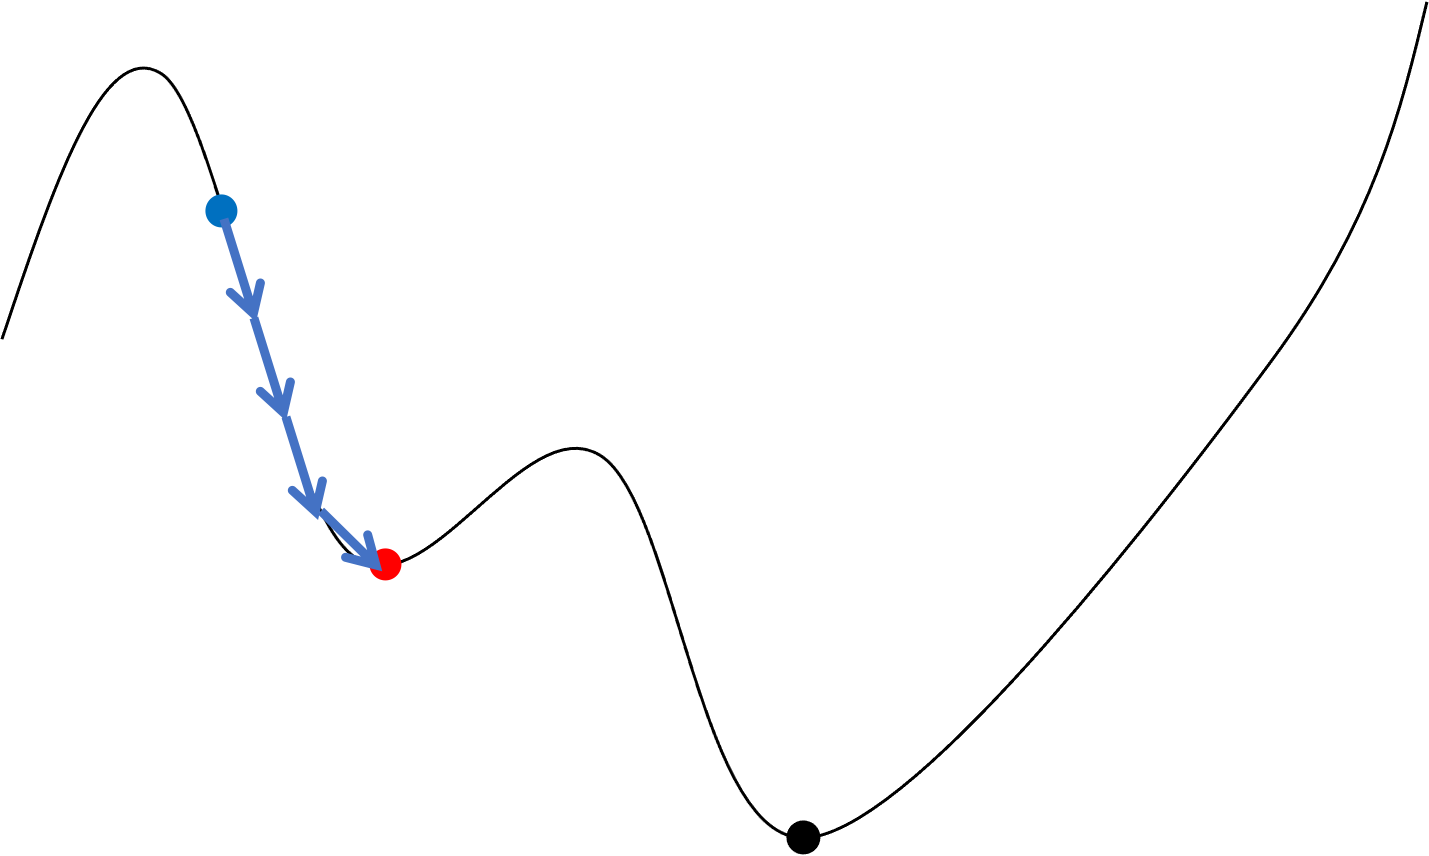
\includegraphics[scale = 0.3]{figures/gradient_descent.png}
    \caption{Illustration of how gradient descent does not always find the global minimum. In the picture, gradient descent initialized at the blue point only makes it to the local minimum at the red point: it does not find the global minimum at the black point.}
    \label{lec10:fig:gradient_descent}
\end{figure}
Before diving into details, we first highlight some observations that will be important to keep in mind when discussing optimization in deep learning. Suppose $g(\theta)$ is the loss function. Recall that the \textit{gradient descent (GD)} algorithm would do the following:
\begin{enumerate}
    \item $\theta_0$ := initialization
    \item $\theta_{t + 1} = \theta_t - \eta\nabla g(\theta_t)$, where $\eta$ is the step size.
\end{enumerate}
Here are some observations to :
\begin{enumerate}
    \item[] \textit{Observation 1}: Gradient descent can find a global minimum for convex functions\footnote{A more precise version of this claim is that gradient descent can find a point that has function value arbitrary close to the global minimal value. } but cannot always find the global minimum for any general continuous functions (see Figure \ref{lec10:fig:gradient_descent} for an illustration).
    \item[] \textit{Observation 2}: Finding the global minimum of general non-convex functions is NP-hard.
%    \item[] \textit{Observation 3}: Gradient descent .
    \item[] \textit{Observation 3}: The objective function in deep learning is non-convex., but empirically gradient descent/stochastic gradient descent typically finds an approximate global minimum of loss function in deep learning.
\end{enumerate}

These observations motivate the following two-step plan:

\begin{enumerate}
    \item Identify a large set of functions that stochastic gradient descent/gradient descent can solve.
    \item Prove that some of the loss functions in machine learning problems belong to this set. (Most of the effort will be spent here.)
\end{enumerate}
\textbf{Basic idea:} Gradient descent can find local minimum $+$ all local minima of $f$ are also global $\Rightarrow$ Gradient descent can find global minima.

\sec{Efficient convergence to (approximate) local minima} \label{sec:optim_convergence}
Let $f$ be a twice-differentiable function. We start with the following definition:
\begin{definition} [Local minimum of a function]
We say that $x$ is a \textit{local minimum} of a function $f$ if there exists an open neighborhood $N$ around $x$ such that in $N$, the function values are at least $f(x)$.
\end{definition}

Note that if $x$ is a local minimum of $f$, then $\nabla f(x) = 0$ and $\nabla^2 f(x) \succeq 0$. However, as the next example shows, the reverse is not true. When $\nabla f(x) = 0$ and $\nabla^2 f(x)$ vanishes in some direction (i.e. merely positive semi-definite instead of being strictly positive definite), higher-order derivatives start to matter.

\begin{example}
\label{lec10:ex:counterexample}
Consider the function $f(x_1, x_2) = x_1^2 + x_2^3$. $(x_1, x_2) = (0, 0)$ satisfies $\nabla f(x) = 0$ and $\nabla^2 f(x)|_{(x_1, x_2) = (0, 0)} = \begin{bmatrix} 2 & 0 \\
0 & 0\end{bmatrix} \succeq 0$. However, if we move in the negative direction of $x_2$, we can decrease the function value. Hence, this example shows why $\nabla f(x) = 0$ and $\nabla^2 f(x) \succeq 0$ does not imply that $x$ is a local minimum.
\end{example}

It is generally not easy to verify if a point is a local minimum. In fact, we have the following theorem regarding the computational tractability:
\begin{theorem}
\label{lec10:thm:np_hard}
It is NP-hard to check whether a point is a local minimum or not \cite{murty1987}. In addition, Hillar and Lim \cite{hillar2013} show that a degree four polynomial is NP-hard to optimize.
\end{theorem}

\subsec{Strict-saddle condition}
Theorem~\ref{lec10:thm:np_hard} forces us to consider more specific types of functions to be able to obtain computational tractability. To this end, we define the following \textit{strict-saddle condition}:

\begin{definition} [Strict-saddle condition \cite{lee2016}]
For positive $\alpha, \beta, \gamma$, we say that $f: \R^d \mapsto \R$ is \textit{$(\alpha, \beta, \gamma)$-strict-saddle} if every $x \in \bbR^d$ satisfies one of the following:
\begin{enumerate}
    \item $\|\nabla f(x)\|_2 \geq \alpha$.
    \item $\lambda_{\min}(\nabla^2 f(x)) \leq -\beta$.
    \item $x$ is $\gamma$-close to a local minimum $x^*$ in Euclidean distance, i.e. $\|x - x^*\|_2 \leq \gamma$.
\end{enumerate}
\end{definition}

Intuitively speaking, this definition is saying if a point has zero gradient and positive semi-definite Hessian, it must be close to a local minimum, i.e. there is no pathological case like Example \ref{lec10:ex:counterexample}.

We have the following theorem for functions that satisfy strict-saddle condition:

\begin{theorem} [Informally stated]
If $f$ is $(\alpha, \beta, \gamma)$-strict-saddle for some positive $\alpha, \beta, \gamma$, then many optimizers (e.g. gradient descent, stochastic gradient descent, cubic regularization) can converge to a local minimum with $\epsilon$-error in Euclidean distance in time $poly \left(d, \frac{1}{\alpha}, \frac{1}{\beta}, \frac{1}{\gamma}, \frac{1}{\epsilon}\right)$.
\end{theorem}

Therefore, if all local minima are global minima and the function satisfies the strict-saddle condition, then optimizers can converge to a global minimum with $\epsilon$-error in polynomial time. (See Figure \ref{lec10:fig:strict-saddle} for an example of a function whose local minima are all global minima.) The next theorem expresses this concretely by being explicit about the strict-saddle condition:

\begin{theorem}
Suppose $f$ is a function that satisfies the following condition: $\exists  \ \epsilon_0, \tau_0, c > 0$ such that if $x \in \bbR^d$ satisfies $\|\nabla f(x)\|_2 \leq \epsilon < \epsilon_0$ and $\nabla^2 f(x) \succeq -\tau_0I$, then $x$ is $\epsilon^c$-close to a global minimum of $f$. Then many optimizers can converge to a global minimum of $f$ up to $\delta$-error in Euclidean distance in time $poly\left(\frac{1}{\delta}, \frac{1}{\tau_0}, d \right)$.
\end{theorem}

\begin{figure}[ht!]
    \centering
    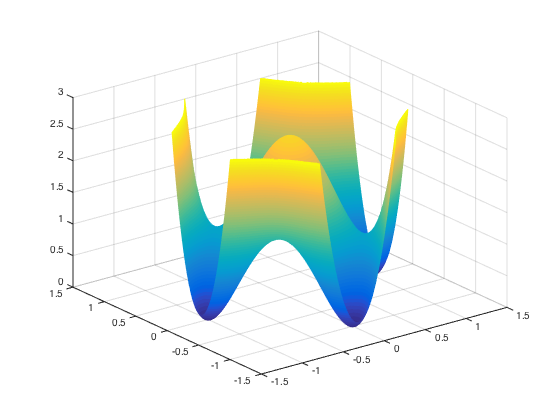
\includegraphics[scale = 0.5]{figures/localmin.png}
    \caption{A two-dimensional function with the property that all local minima are global minima. It also satisfies the strict-saddle condition because all the saddle points have a strictly negative curvature in some direction.}
    \label{lec10:fig:strict-saddle}
\end{figure}

\sec{All local minima are global minima: two examples} \label{sec:two_optim_examples}
So far, we have focused on general results. Next, we give two concrete examples that have the property that all local minima are global minima: (i) principal components analysis (PCA)/matrix factorization/linearized neural nets, and (ii) matrix completion. \tnote{need some quick literature survey; Tengyu will add}%There is a rich literature on this topic and 

\subsec{Principal components analysis (PCA)}
Let matrix $M \in \bbR^{d \times d}$ be symmetric and positive semi-definite. Consider the problem of finding the best rank-1 approximation of the matrix $M$. The objective function here is non-convex:
\begin{equation}
    \min_{x \in \bbR^d}g(x) \triangleq \frac{1}{2}\|M - xx^\top \|_F^2.
\end{equation}

\begin{theorem}
All local minima of $g$ are global minima (even though $g$ is non-convex).
\end{theorem}

\begin{remark}
For $d = 1$, $g(x) = \frac{1}{2}(m - x^2)^2$ for some constant $m$. Figure~\ref{lec10:fig:pca_objective} below shows such an example. We can see that all local minima are indeed global minima.
\end{remark}

\begin{figure}[ht!]
    \centering
    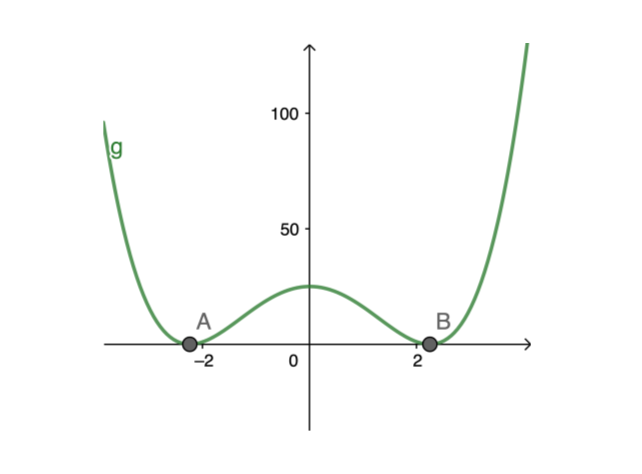
\includegraphics[scale = 0.4]{figures/pca.png}
    \caption{Objective function for principal components analysis (PCA) when $d = 1$.}
    \label{lec10:fig:pca_objective}
\end{figure}

\begin{proof}

\textit{Step 1: Show that all stationary points must be eigenvectors.} From HW0, we know that $\nabla g(x) = -(M - xx^\top )x$, hence
\begin{equation}\label{lec10:eqn:pca-firstorder}
\nabla g(x) = 0 \implies Mx = \|x\|_2^2\cdot x,
\end{equation}
which implies that $x$ is an eigenvector of $M$ with eigenvalue $\|x\|_2^2$. From the Eckart–Young–Mirsky theorem we know the global minimum (i.e. the best rank-1 approximation) is the eigenvector with the largest eigenvalue.

\textit{Step 2: Show that all local minima must be eigenvectors of the largest eigenvalue.} We use the second order condition for this. For $x$ to be a local minimum we need $\nabla^2g(x) \succeq 0$, which means for any $v \in  \bbR^d$, 
\begin{equation}
\langle v, \nabla^2g(x) v \rangle \geq 0.
\end{equation}
To compute $\langle v, \nabla^2g(x) v \rangle$, we use the following trick: expand $g(x + v)$ into $g(x) + \text{linear term in } v + \text{quadratic term in } v$, then the quadratic term will be $\frac{1}{2}\langle v, \nabla^2g(x) v \rangle$ (see HW0 Problem 2d for an example). Using this trick, we get 

\begin{align}
    g(x+v) &= \frac{1}{2}\|M - (x+v)(x+v)^\top \|_F^2 \\
           &= \frac{1}{2}\|M-xx^\top\|_F^2 - \langle M-xx^\top , xv^\top + vx^\top\rangle + \frac{1}{2}\langle xv^\top + vx^\top , xv^\top + vx^\top \rangle \nonumber \\
          & \quad -\langle M-xx^\top, vv^\top\rangle + \text{higher order terms in }v.
\end{align}
Hence, we have 
\begin{align}
    \frac{1}{2}\langle v, \nabla^2g(x) v \rangle & = \frac{1}{2}\langle xv^\top + vx^\top, xv^\top + vx^\top \rangle
          -\langle M-xx^\top, vv^\top\rangle  \\
          &= \langle x, v\rangle^2 + \|x\|_2^2\|v\|_2^2 - v^ Mv + \langle x, v\rangle^2 \\
          & = 2\langle x, v\rangle^2 + \|x\|_2^2\|v\|_2^2 - v^\top Mv.
\end{align}

Picking $v = v_1$, the unit eigenvector with the largest eigenvalue (denoted $\lambda_1$), for $x$ to be a local minimum it must satisfy 
\begin{equation}
\langle v_1, \nabla^2g(x) v_1 \rangle = 2\langle x, v_1 \rangle^2 - v_1^\top Mv_1 + \|x\|_2^2 \geq 0.
\end{equation}

Note that by \eqref{lec10:eqn:pca-firstorder}, all our candidates for local minima are eigenvectors of $M$ so naturally we have two cases:
\begin{itemize}
\item \textit{Case 1: $x$ has eigenvalue $\lambda_1$}. Then x is the global minimum (by the Eckart–Young–Mirsky theorem).
\item \textit{Case 2: $x$ has eigenvalue $\lambda < \lambda_1$}. Then we know $x$ and $v_1$ are orthogonal (eigenvectors with different eigenvalues are always orthogonal), hence 
\begin{equation}
2\langle x, v_1 \rangle^2 - v_1^\top Mv_1 + \|x\|_2^2 = 0  -\lambda_1 + \lambda \geq 0,
\end{equation}
which implies $\lambda \geq \lambda_1$, a contradiction. 
\end{itemize}

In summary, if $x$ is a stationary point and $x$ is not a global minimum, then moving in the direction of $v_1$ would lead to second-order improvement and $x$ cannot be a local minimum. 
\end{proof}

	% reset section counter
%\setcounter{section}{0}

%\metadata{lecture ID}{Your names}{date}
\metadata{11}{Andrew Wang}{Feb 22nd, 2021}

\subsec{Matrix Completion \texorpdfstring{\cite{ge2016}}{[Ge et al., 2016]}}
We consider rank-1 matrix completion for simplicity. Let $M = zz^\top$ be a rank-1 symmetric and positive semi-definite matrix for some $z\in \bbR^d$. Given random entries of $M$, our goal is to recover the rest of entries. Formally, we have the following definitions:

\begin{definition}
Suppose $M\in \bbR^{d\times d}$ and $\Omega \subseteq [d] \times [d]$, we define $P_{\Omega}(M)$ to be the matrix obtained by zeroing out every entry outside $\Omega$. 
\end{definition}

\begin{definition}[Matrix Completion]
Suppose $M\in \bbR^{d\times d}$ and every entry of $M$ is included in $\Omega$ with probability $p$. The \textit{matrix completion task} is to recover $M$ (with respect to some loss functions) given the observation $P_{\Omega}(M)$.
\end{definition}

A nice real world example of matrix completion is when we have a matrix describing the user ratings for each item. We only observe a small portion of the entries as each customer only buys a small subset of the items. A good matrix completion algorithm is indispensable for a recommendation engine. 

\begin{remark}
We need $d$ parameters to describe a rank-1 matrix $M$ and the number of observations is roughly $pd^2$. Thus, for identifiability we need to work in the regime where $pd^2 > d$, i.e. $p \gg \frac{1}{d}$. 
\end{remark}

We define our non-convex loss functions to be 
\begin{align}
    \min_{x \in \bbR^d} f(x) & \triangleq \frac{1}{2}\sum_{(i,j)\in \Omega}(M_{ij}-x_ix_j)^2 \\
     & = \frac{1}{2}\|P_{\Omega}(M-xx^\top)\|_F^2.
\end{align}

To really solve our problem we need some regularity condition on the ground truth vector $z$ (recall $M = zz^\top$). \textit{Incoherence} is one such condition:
\begin{definition}[Incoherence]
Without loss of generality, assume the ground truth vector $z\in\bbR^d$ satisfies $\|z\|_2 = 1$. $z$ satisfies the \textit{incoherence condition} if $\|z\|_{\infty} \leq \frac{\mu}{\sqrt{d}}$, where $\mu$ is considered to be a constant or log in dimension $d$. 
\end{definition}

\begin{remark}
A nice counterexample to think about why such condition is necessary is when $z = e_1$ and $M = e_1 e_1^\top$. All entries of $M$ are 0 except for a 1 in the top-left corner. There is no way to recover $M$ without observing the top-left corner.
\end{remark}

The goal is to prove that local minima of this objective function are close to a global minimum:

\begin{theorem}\label{lec11:thm:matrix-completion}
Assume $p = \dfrac{\textrm{poly}(\mu, \log d)}{d\epsilon^2}$ for some sufficient small constant $\epsilon$ and assume $z$ is incoherent. Then with high probability, all local minima of $f$ are $O(\sqrt{\epsilon})$-close to $+z$ or $-z$ (the global minima of $f$).
\end{theorem}

Before presenting the proof, we make some observations that will guide the proof strategy.

\begin{remark}
$f(x)$ can be viewed as a sampled version of the PCA loss function $g(x) = \frac{1}{2}\norm{M - xx^\top}_F^2 = \frac{1}{2}\sum_{(i,j) \in [d]\times[d]} (M_{ij} - x_ix_j)^2$, in which we only observe a subset of the matrix entries. Thus, we would like to claim that $f(x) \approx g(x)$. However, matching the values of $f$ and $g$ is not sufficient to prove the theorem: even a small margin of error between $f$ and $g$ could lead to creation of many spurious local minima (see Figure~\ref{lec11:fig:matrix_completion_f_g} for an illustration). In order to ensure that the local minima of $f$ look like the local minima of $g$, we will need further conditions like $\nabla f(x) \approx \nabla g(x)$ and $\nabla^2 f(x) \approx \nabla^2 g(x)$.
\end{remark}

\begin{figure}
    \centering
    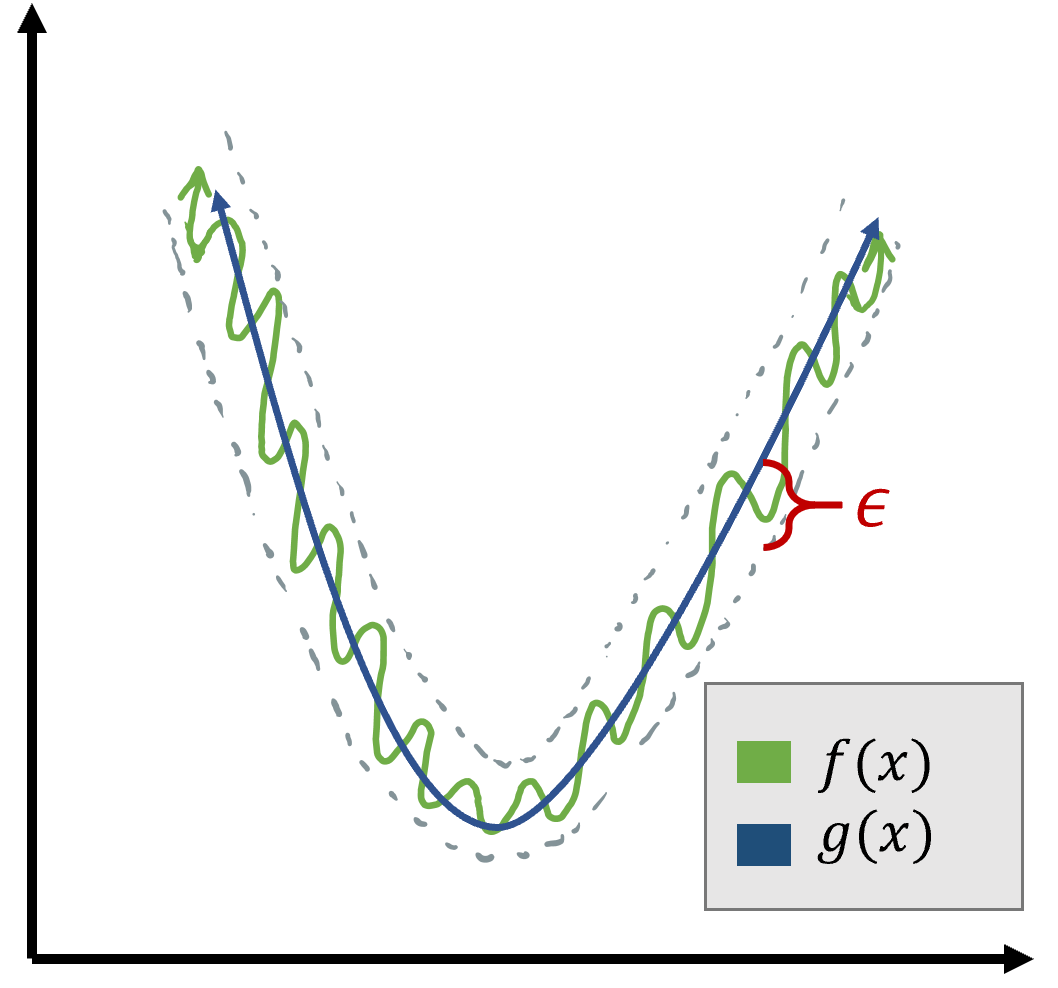
\includegraphics[width=2.5in]{figures/matrix-completion-f-g.png}
    \caption{Even if $f(x)$ and $g(x)$ are no more than $\epsilon$ apart at any given $x$, without any additional knowledge, the local minima of $f$ may possibly look dramatically different from the local minima of $g$. However, the proofs in this section show that the landscape of $f$ (the matrix completion objective) and $g$ (the PCA objective) are have similar properties by proving more advanced concentration inequalities. }
    \label{lec11:fig:matrix_completion_f_g}
\end{figure}

\begin{remark}
Key idea: concentration for scalars is easy. We can approximate a sum of scalars via a sample:
\begin{equation}
\sum_{(i,j) \in \Omega} T_{ij} \approx p\sum_{(i,j) \in [d]\times[d]} T_{ij},
\end{equation}
where we use $\approx$ to mean that
\begin{equation}
\Bigl| \sum_{(i,j) \in \Omega} T_{ij} - p\sum_{(i,j) \in [d]\times[d]} T_{ij} \Bigr| < \epsilon
\end{equation}
with high probability. This suggests the strategy of casting the estimation of our desired quantities in the form of estimating a scalar sum via a sample. In particular, we note that for any matrices $A$ and $B$,
\begin{equation}
\langle A, P_\Omega(B) \rangle = \sum_{(i,j) \in \Omega} A_{ij}B_{ij} \approx p\langle A, B \rangle.
\end{equation}
\end{remark}

To make use of this observation to understand the quantities of interest ($\nabla f(x)$ and $\nabla^2 f(x)$), we compute the bilinear and quadratic forms for $\nabla f(x)$ and $\nabla^2 f(x)$ respectively:
\begin{equation}
\langle v, \nabla f(x) \rangle = \langle v, P_\Omega(M-xx^\top)x \rangle = \langle vx^\top, P_\Omega(M-xx^\top) \rangle,
\end{equation}
where we have used the fact that $\langle A,BC \rangle = \langle AC^\top,B\rangle$. Also note that $vx^\top$ is a rank-1 matrix and $M-xx^\top$ is a rank-2 matrix.
\begin{align}
\langle v, \nabla^2 f(x) v \rangle &= \norm{P_\Omega(vx^\top + xv^\top)}_F^2 - 2\langle P_\Omega(M-xx^\top), vv^\top \rangle \\
&=  \langle P_\Omega(vx^\top + xv^\top), vx^\top + xv^\top \rangle - 2\langle P_\Omega(M-xx^\top), vv^\top \rangle,
\end{align}

where we have used the fact that $\norm{P_\Omega(A)}_F^2 = \langle P_\Omega(A), P_\Omega(A)\rangle = \langle P(\Omega(A), A\rangle$.

The key lemma that applies the scalar concentration to these matrix quantities is as follows:

\begin{lemma}
Let $\epsilon>0$, $p = \dfrac{\textrm{poly}(\mu, \log d)}{d\epsilon^2}$. Given that $A = uu^\top, B=vv^\top$ for some $u, v$ satisfying $\norm{u}_2 \leq 1$, $\norm{v}_2 \leq 1$, $\norm{u}_\infty \leq \mu / \sqrt{d}$, $\norm{v}_\infty \leq \mu / \sqrt{d}$, we have $|\langle P_\Omega(A), B \rangle/p - \langle A, B\rangle| \leq \epsilon$ w.h.p.
\label{lec11:lem:concentration_lemma}
\end{lemma}

If we can show that $g$ has no bad local minima via a proof that only uses $g$ via terms of the form $\langle v, \nabla g(x) \rangle$ and $\langle v, \nabla^2 g(x) v \rangle$, then by Lemma~\ref{lec11:lem:concentration_lemma} this proof will automatically generalize to $f$ by concentration.

Next, we prove some facts about $g$ and show the analogous proofs for $f$ that we will use in the proof of Theorem~\ref{lec11:thm:matrix-completion}.

\begin{lemma}[Connecting inner product and norm for $g$]\label{lec11:lem:inner-g}
If $x$ satisfies $\nabla g(x) = 0$, then $\langle x,z \rangle^2 = \norm{x}_2^4$.
\end{lemma}

\begin{proof}
\begin{align}
    \nabla g(x) = 0 &\implies \langle x, \nabla g(x) \rangle = 0 \\
   & \implies \langle x, (zz^\top-xx^\top)x \rangle = 0 & (\because \nabla g(x) = (M - xx^\top)x) \\
   & \implies \langle x,z \rangle^2 = \norm{x}_2^4.
\end{align}
\end{proof}

\begin{lemma}[Connecting inner product and norm for $f$]\label{lec11:lem:inner-f}
Suppose $\norm{x}_\infty \leq 2\mu / \sqrt{d}$. If $x$ satisfies $\nabla f(x) = 0$, then $\langle x,z \rangle^2 \geq \norm{x}_2^4 - \epsilon$ with high probability.
\label{inner_prod_norm_f}
\end{lemma}

\begin{proof}
\begin{align}
    \nabla f(x) = 0 &\implies \langle x, \nabla f(x) \rangle = 0 \\
    & \implies \langle x, \nabla g(x) \rangle \approx \langle x, \nabla f(x) \rangle/p \pm \epsilon & \text{(by Lemma \ref{lec11:lem:concentration_lemma})} \\
   & \implies |\langle x, (zz^\top-xx^\top)x \rangle| \leq \epsilon & \text{w.h.p.} \\
   & \implies \langle x,z \rangle^2 \geq \norm{x}_2^4 - \epsilon & \text{w.h.p.}
\end{align}
\end{proof}

\begin{lemma}[Bound norm for $g$]\label{lec11:lem:bound-g}
    If $\nabla^2 g(x) \succeq 0$, then $\norm{x}_2^2 \geq 1/3$.
\end{lemma}

\begin{proof}
\begin{align}
    \nabla^2 g(x) \succeq 0
    &\implies \langle z, \nabla^2 g(x)z\rangle \geq 0 \\
    &\implies \norm{zx^\top + xz^\top}_F^2 - 2z^\top(zz^\top-xx^\top)z \geq 0 \\
    &\implies 2 \norm{x}^2_2 + 2 \inprod{x, z}^2 - 2 + 2 \inprod{x, z}^2 \geq 0 &\text{(cyclic trace prop.)} \\
    &\implies 3\norm{x}_2^2 = \norm{x}_2^2 + 2\norm{x}_2^2 \geq \norm{x}_2^2 + 2\langle x,z \rangle^2 \geq 1 &\text{(by Cauchy-Schwarz)} \\
    &\implies \norm{x}_2^2 \geq 1/3.
\end{align}
\end{proof}

\begin{lemma}[Bound norm for $f$]\label{lec11:lem:bound-f}
    Suppose $\norm{x}_\infty \leq \mu / \sqrt{d}$. If $\nabla^2 f(x) \succeq 0$, then $\norm{x}_2^2 \geq 1/3 - \epsilon/3$ with high probability.
\end{lemma}
\begin{proof}
\begin{align}
    \nabla^2 f(x) \succeq 0
    &\implies \langle z, \nabla^2 f(x)z \rangle \geq 0 \\
    &\implies \langle z, \nabla^2g(x)z \rangle \geq -\epsilon & \text{w.h.p. (by Lemma \ref{lec11:lem:concentration_lemma})} \\
    &\implies 3\norm{x}_2^2 \geq 1-\epsilon & \text{w.h.p.} \\
    &\implies \norm{x}_2^2 \geq 1/3 - \epsilon/3 & \text{w.h.p.}
\end{align}
\end{proof}

\begin{lemma}[$g$ has no bad local minimum]
    All local minima of $g$ are global minima.
\end{lemma}

\begin{proof}
\begin{align}
    \nabla g(x) = 0
    & \implies \langle z, \nabla g(x) \rangle = 0 \\
    & \implies \langle z, (zz^\top-xx^\top)x \rangle = 0 \\
    & \implies \langle x,z\rangle (1-\norm{x}_2^2) = 0.
\end{align}
Since $|\langle x,z \rangle| \geq 1/3 \neq 0$ (by Lemma~\ref{lec11:lem:bound-g}), we must have $\norm{x}_2^2 = 1$. But then Lemma~\ref{lec11:lem:inner-g} implies $\langle x, z\rangle^2 = \norm{x}_2^4 = 1$, so $x = \pm z$ by Cauchy-Schwarz.
\end{proof}

We now prove Theorem~\ref{lec11:thm:matrix-completion}, restated for convenience:
\begin{theorem}[$f$ has no bad local minimum]
Assume $p = \dfrac{\textrm{poly}(\mu, \log d)}{d\epsilon^2}$. Then with high probability, all local minima of $f$ are $O(\sqrt{\epsilon})$-close to $+z$ or $-z$.
\end{theorem}

\begin{proof}
Observe that $\norm{x-z}_2^2 = \norm{x}_2^2 + \norm{z}_2^2 - 2\langle x,z \rangle \leq \norm{x}_2^2 + 1 - 2\langle x,z \rangle$. Our goal is to show that this quantity is small with high probability, hence we need to bound $\norm{x}_2^2$ and $\langle x,z \rangle$ w.h.p. Note that the following bounds in this proof are understood to hold w.h.p.
    
Let $x$ be such that $\nabla f(x) = 0$. For $\epsilon \leq 1/16$,
\begin{align}
\langle x,z \rangle^2 &\geq \norm{x}_2^4 - \epsilon &\text{(by Lemma~\ref{lec11:lem:inner-f})} \\
&\geq (1/3-\epsilon/3)^2 - \epsilon &\text{(by Lemma~\ref{lec11:lem:bound-f})} \\
&\geq 1/32. \label{lec11:eqn:xz-bound}
\end{align}

With this, we can get a bound on $\norm{x}_2^2$:
\begin{align}
\nabla f(x) = 0 &\implies \langle x, \nabla f(x) \rangle = 0 \\
&\implies |\langle z, \nabla g(x) \rangle| \leq \epsilon & \text{(by Lemma \ref{lec11:lem:concentration_lemma})} \\
&\implies |\langle x,z\rangle| \cdot |1-\norm{x}_2^2| \leq \epsilon &\text{(by dfn of $g$)} \\
&\implies |1-\norm{x}_2^2| \leq 32\epsilon = O(\epsilon) &\text{(by \eqref{lec11:eqn:xz-bound})} \\
&\implies \norm{x}_2^2 = 1 \pm O(\epsilon). \label{lec11:eqn:xnorm-bound}
\end{align}
    
Next, we bound $\langle x,z \rangle$:
\begin{align}
\langle x, z \rangle^2 &\geq \norm{x}_2^4 - \epsilon &\text{(by Lemma \ref{inner_prod_norm_f})} \\
&\geq (1-O(\epsilon))^2 - \epsilon &\text{(by \eqref{lec11:eqn:xnorm-bound})} \\
&= 1 - O(\epsilon).
\end{align}

Finally, we put these quantities together to bound $\norm{x-z}_2^2$. We have two cases:
    
\textbf{Case 1}: $\langle x,z\rangle \geq 1 - O(\epsilon)$. Then
\begin{align}
\norm{x-z}_2^2 &= \norm{x}_2^2 + \norm{z}_2^2 - 2\langle x,z \rangle \\
&\leq \norm{x}_2^2 + 1 - 2\langle x,z \rangle \\
&\leq 1 + O(\epsilon) + 1 - 2(1-O(\epsilon)) \\
&\leq O(\epsilon).
\end{align} 
    
Hence we conclude $x$ is $O(\sqrt{\epsilon})$-close to $z$.
    
\textbf{Case 2}: $\langle x,z\rangle \leq -(1 - O(\epsilon))$. Then by an analogous argument, $x$ is $O(\sqrt{\epsilon})$-close to $-z$.
\end{proof}

We have shown above that matrix completion of a rank-1 matrix has no spurious local minima. This proof strategy can be extended to handle higher-rank matrices and noisy matrices \cite{ge2016}. The proof also demonstrates a generally useful proof strategy: often, reducing a hard problem to an easy problem results in solutions that do not give much insight into the original problem, because the proof techniques do not generalize. It can often be fruitful to seek a proof in the simplified problem that makes use of a restricted set of tools that could generalize to the harder problem. Here we limited ourselves to only using $\langle v, \nabla g(x)\rangle$ and $\langle v, \nabla^2 g(x) v\rangle$ in the easy case; these quantities could then be easily converted to analogous quantities in $f$ via the concentration lemma (Lemma~\ref{lec11:lem:concentration_lemma}).

\subsec{Other problems where all local minima are global minima}
We have now demonstrated that two classes of machine learning problems, rank-1 PCA and rank-1 matrix completion, have no spurious local minima and are thus amenable to being solvable by gradient descent methods. We now outline some major classes of problems for which it is known that there are no spurious local minima.

\begin{itemize}
    \item Principal component analysis (covered in previous lecture).
    \item Matrix completion (and other matrix factorization problems). On a related note, it has also been shown that linearized neural networks of the form $y = W_1W_2x$, where $W_1$ and $W_2$ are optimized separately, have no spurious local minima \cite{baldi1989neural}. It should be noted that linearized neural networks are not very useful in practice since the advantage of optimizing $W_1$ and $W_2$ separately versus optimizing a single $W=W_1W_2$ is not clear.
    \item Tensor decomposition. The problem is as follows:
    \begin{align}
        \text{maximize }\quad \sum_{i=1}^d \sum_{j=1}^d \sum_{k=1}^d \sum_{l=1}^d T_{ijkl} x_ix_jx_kx_l \quad \text{such that } \quad \norm{x}_2 = 1.
    \end{align}
    Additionally, constraints are imposed on the tensor $T$ to make the problem tractable. For example, one condition is that $T$ must be a low-rank tensor with orthonormal components \cite{ge2015}.
\end{itemize}
	% reset section counter
%\setcounter{section}{0}

%\metadata{lecture ID}{Your names}{date}
\metadata{12}{Rohan Taori and Jonathan Lee}{Feb 24nd, 2021}

\sec{Neural tangent kernel (NTK) approach}
In general, the loss landscapes of neural networks (with nonlinearities) is currently not as well understood. We now introduce the \textit{neural tangent kernel} which allows us to make some characterizations of the loss near a given neural network initialization.

\begin{figure}
    \centering
    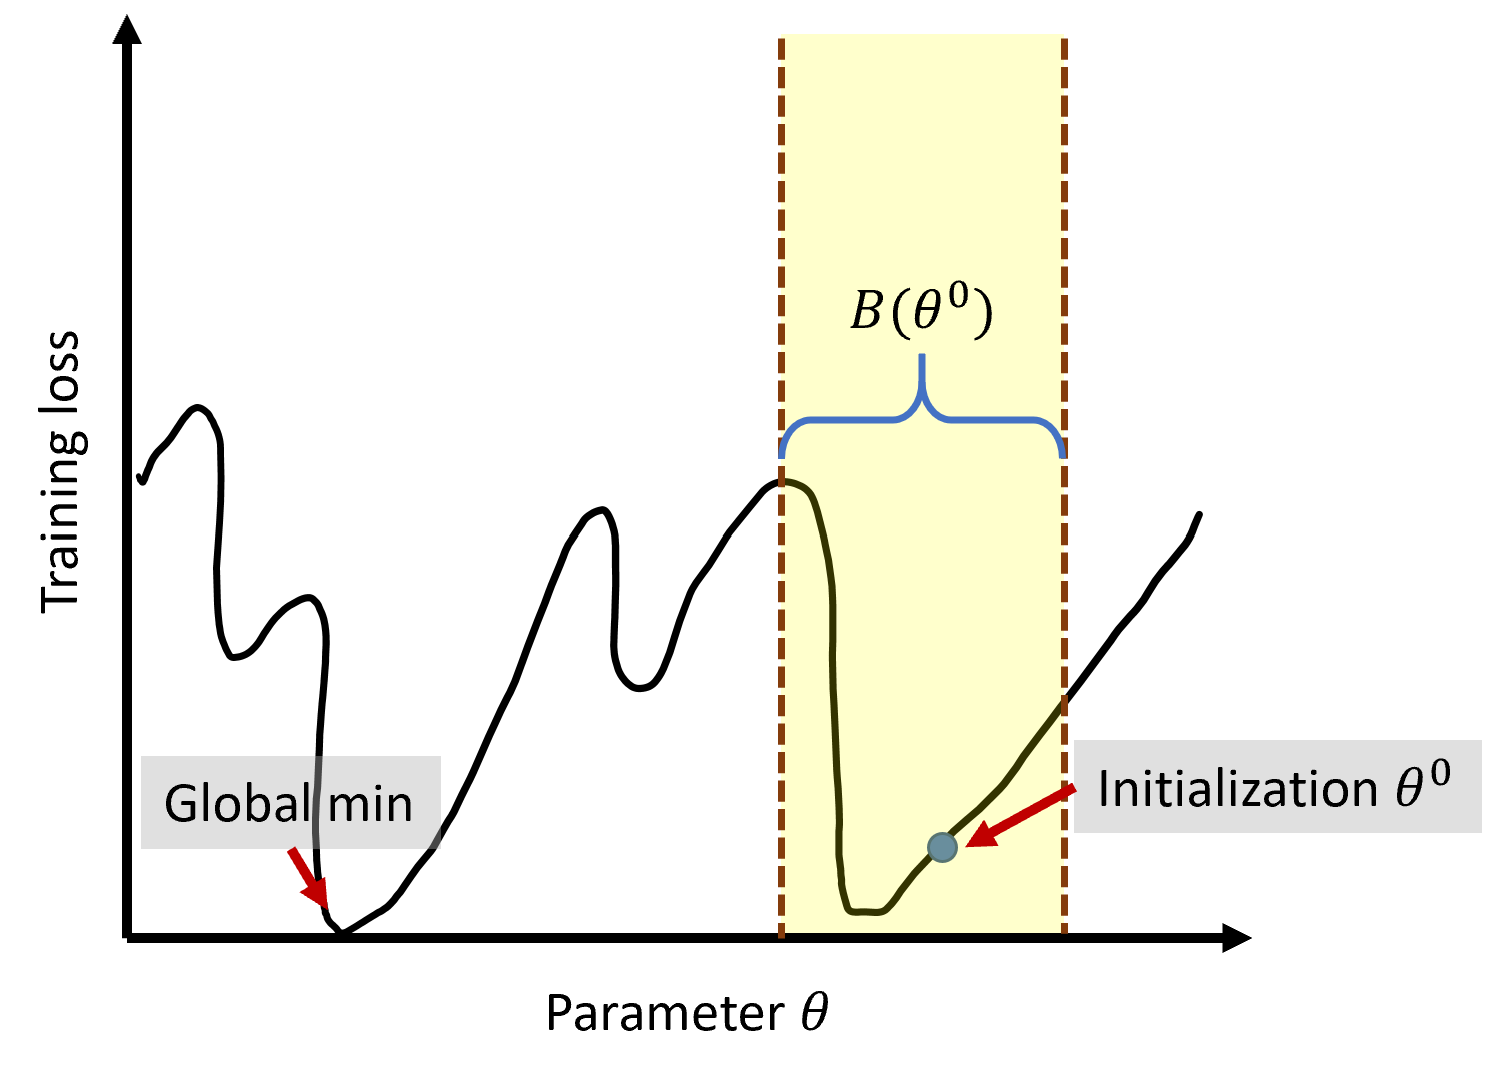
\includegraphics[width=2.5in]{figures/ntk-loss-landscape.png}
    \caption{The training loss landscape around a given parameter initialization $\theta^0$. We hope that the neighborhood around $\theta^0$ contains a local minimum that is close to the global minimum.}
    \label{lec11:fig:ntk_loss_landscape}
\end{figure}

The key insight of the NTK approach is that if we take an appropriate random parameter initialization $\theta^0$ (which we will choose later), we can identify a special neighborhood of $\theta^0$, denoted $B(\theta^0)$, where ``everything is nice''. That is, the function is convex in $B(\theta^0)$, there is a global minimum in the $B(\theta^0)$, and the algorithm starting at $\theta^0$ will converge to that global minimum. (See Figure~\ref{lec11:fig:ntk_loss_landscape} for an illustration.)

Take a random initialization $\theta = \theta^0$ and Taylor expand the loss around $\theta^0$ w.r.t. $\theta$:
\begin{align}
f_\theta(x) &= \underbrace{f_{\theta^0}(x) + \langle \nabla_\theta f_{\theta^0}(x), \theta - \theta^0 \rangle}_{g_\theta(x)} + O((\theta-\theta^0)^2).
\end{align}

In other words, we take the tangent plane to $f_\theta$ at $x$ (a linear approximation). We observe that $g_\theta$ is an affine function of $\theta$. Additionally, defining $\Delta \theta = \theta - \theta^0$, we see that the first term does not depend on $\Delta \theta$ while the second term $\langle \nabla_\theta f_{\theta^0}(x), \theta - \theta^0 \rangle$ is linear in $\Delta \theta$. (For convenience, we will sometimes choose to design $\theta^0$ such that $f_{\theta^0}(x) = 0$ so that $g_\theta$ is linear in $\theta^0$. However, the difference is not very important since $f_{\theta^0}(x)$ can simply be subsumed in the training labels $y$ via $y' = y - f_{\theta^0}(x)$.)

Now we have that $y \approx \nabla_\theta f_{\theta^0}(x)^T \Delta \theta$. We can view $\phi(x) \triangleq \nabla_\theta f_{\theta^0}(x)$ as a feature map, i.e. we can rewrite the expression as $\phi(x)^T \Delta \theta$ where $\phi(x)$ is fixed (only depends on $\theta^0$ and the architecture). This observation motivates the definition of the \textit{neural tangent kernel}:

\begin{definition}[Neural tangent kernel]
The \emph{neural tangent kernel} $K$ is defined as the function
\begin{equation}
K(x, x') = \langle \phi(x), \phi(x')\rangle = \langle \nabla f_{\theta^0}(x), \nabla f_{\theta^0}(x') \rangle.
\end{equation}
\end{definition}

Suppose we fit $g_\theta(x)$ to $y$, i.e. we minimize the loss 
\begin{equation}
\textrm{Loss} = \ell(\phi(x)^T \Delta \theta, y),
\end{equation}
where $\phi(x)^T\Delta \theta$ is linear and the loss as a whole is convex.
We will show that for a sufficiently wide neural network with proper initialization $\theta^0$, optimizing $f_\theta(x)$ starting from $\theta^0$ never leaves the neighborhood of $\theta^0$, effectively behaving the same as optimizing $g_\theta(x)$. In particular, two questions have to be answered:

\begin{enumerate}
    \item \textit{Why does there exist a small neighborhood $B(\theta^0)$ such that there exists a global minimum in $B(\theta^0)$?} This is more surprising, and it involves proper design of $\theta^0$. We will spend the rest of this chapter answering this question mathematically.
    \item \textit{Does gradient descent on the original loss with respect to $f_\theta(x)$ stay in the neighborhood $B(\theta^0)$?} The answer to this question is ``yes''. However, more technical machinery is required to prove it. We skip discussion of this as it is the less surprising claim.
\end{enumerate}

\subsec{The two-layer network case}

We demonstrate the NTK approach for the two-layer network setup. For $i \in [m]$, let $a_i \in \R$ be scalars and let $w_i \in \R^d$ be vectors. Let $\sigma: \R \to \R$ be the ReLU activation function defined as $\sigma(t) = \max\{ t, 0\}$. Suppose we have the following two-layer network:
\begin{equation}\label{lec12:eqn:network}
\hat{y} = f_\theta(x) = \frac{1}{\sqrt{m}} \sum_{i=1}^m a_i \sigma (w_i^\top x),
\end{equation}
for some input $x$.

Our weight matrix is $W = \begin{bmatrix} w_1^\top \\ \vdots \\ w_m^\top \end{bmatrix} \in \R^{m \times d}$. We initialize $W$ randomly using $W_{ij} \stackrel{i.i.d.}{\sim} \mathcal{N}(0, 1)$ for all $i$ and $j$. We initialize $a_i \in \{\pm 1\}$ and assume that the $a_i$'s are fixed after initialization, i.e. not updated during training. (We fix $a_i$ for simplicity: the results still hold when we are allowed to optimize $a_i$ in training.) We also assume that $x$ has norm on the order of $1$, and that the true label $y$ is on the order of $1$.

In our analysis, we will assume we have sufficiently large $m = \poly(n, d)$. In other words, the width of the network $m$ is sufficiently large such that $\poly(n, d)$ factors are not important in the analysis. For simplicity, we write $O_{d,n}(1)$ to hide polynomial dependencies on $d$ and $n$. Thus $O_{d,n}(m^c) = m^c \cdot \poly(n, d)$.

\textbf{Why do we need the scaling factor $1 / \sqrt{m}$ in Equation~\eqref{lec12:eqn:network}?} It is included to prevent the model outputs from blowing up when we increase the number of neurons $m$. Note that $\sigma (w_i^\top x) \approx O_{d,n}(1)$ since $w_i^\top \approx O_{d,n}(1)$ and $x \approx O_{d,n}(1)$. Since $a_i \in \{ \pm 1\}$ for all $i$, this implies that $ \sum_{i=1}^m a_i \sigma (w_i^\top x) \approx O_{d,n}(\sqrt{m})$. Thus, the scaling factor is needed to obtain $\hat{y} = f_\theta(x) = O_{d,n}(1)$.

Next, we introduce some notation that will be helpful for our analysis. Let $\Delta \theta = \theta - \thetazero$. Suppose we have $n$ examples $x^{(1)},...,x^{(n)}$ and labels $y^{(1)},...,y^{(n)}$. Let $\vec{y} = \begin{bmatrix} y^{(1)} & \dots & y^{(n)} \end{bmatrix}^\top$. Let
\begin{equation}
\vec{y'} = \begin{bmatrix} y^{(1)}-f_{\thetazero}(x^{(1)}) \\ \vdots \\ y^{(n)}-f_{\thetazero}(x^{(n)}) \end{bmatrix}
\end{equation}
be the transformed labels where we subsume the affine term in the label, allowing us to treat this as a purely linear model without loss of generality. Note that $\theta = \text{vec}(W) \in \R^{dm}$ is the vectorized version of the weights. Let $\Phi^{(i)} = \nabla_\theta f_{\thetazero}(x^{(i)}) \in R^{dm}$ be the feature associated with the $i$th example, and let $\Phi$ denote the collection of the features across the examples:
\begin{equation}
\Phi = \begin{bmatrix} \Phi^{(1)^\top} \\ \vdots \\ \Phi^{(n)^\top} \end{bmatrix} \in R^{n \times dm}.
\end{equation}

Recall that we defined
\begin{align}
    g_\theta(x) = f_{\thetazero}(x) + \langle\nabla_\theta f_{\thetazero}, \theta - \thetazero\rangle,
\end{align}
which is the linear approximation of $f_\theta(x)$ at $\thetazero$. If we wish to fit $g_\theta(x)$ to $y$ with the $\ell_2$-loss, we may consider minimizing the following objective function over $\theta$:
\begin{align}
\sum_{i=1}^n \left( y^{(i)} - f_{\thetazero}(x^{(i)}) - \langle \nabla_\theta f_{\thetazero}(x\sp{i}), \theta - \thetazero \rangle \right)^2 
&=  \sum_{i=1}^n \left(y^{(i)} - f_{\thetazero}(x^{(i)}) - \Delta\theta^\top \Phi^{(i)} \right)^2 \\
&=  \norm{\vec{y'} - \Phi \Delta\theta}_2^2.
\end{align}
This is equivalent to the following optimization problem:
\begin{align}
    \min_{\Delta \theta} \quad \norm{\vec{y'} - \Phi \Delta\theta}_2^2. \label{lec12:eqn:opt-problem}
\end{align}
Since $n \ll dm$, so we have an undetermined linear system. Since our goal is to show that the relevant neighborhood around $\thetazero$ is small, we should choose the minimum norm solution which can be found directly by the pseudoinverse: $\hat{\theta} = \Phi^\dagger \vec{y'}$,  where $\Phi^\dagger$ is the pseudoinverse of $\Phi$ given by $\Phi^\dagger = \Phi^\top (\Phi \Phi^\top)^{-1}$.

It remains to show that the norm of $\hat{\theta}$ is small. Before we can do that, we will prove some useful claims:

\begin{lemma}[$\Phi$ is a well-conditioned matrix]\label{lec12:lem:claim1}
When $\thetazero$ is random, $\Phi$ is well-conditioned in the sense that \begin{align}
\sigma_{\min}(\Phi) \approx \frac{1}{\sqrt{n}} \norm{\Phi}_F \quad \text{and} \quad
\sigma_{\max}(\Phi) \approx \frac{1}{\sqrt{n}} \norm{\Phi}_F.
\end{align}
($\sigma_{\min}(\Phi)$ and $\sigma_{\max}(\Phi)$ denote the smallest and largest singular values of $\Phi$ respectively.) Specifically, $\sigma_{min}(\Phi) \gtrsim \Omega \left( \frac{1}{\sqrt{n}} \norm{\Phi}_F \right)$, and vice-versa for $\sigma_{\max}(\Phi)$.
{\color{blue} Note: this lemma is very problematic and perhaps outright wrong. It will be updated in the next revision} \tnoteimp{Tengyu will fix this}
\end{lemma}

We omit the proof as it uses tools from random matrix theory that are not required for this course. (The high-level idea is to show that $\Phi \Phi^\top \approx c \cdot I$ for some constant scalar $c$.)

\begin{remark}
Since $\Phi \in R^{n \times dm}$, $\Phi$ has at most $n$ singular values $\sigma_1 \geq \ldots \geq \sigma_n \geq 0$. Since $\norm{\Phi}_F = \sqrt{\sigma_1^2 + ... + \sigma_n^2}$, the fact that $\sigma_n \approx \frac{1}{\sqrt{n}} \norm{\Phi}_F$ means that all the singular values are not very different from each other.
\end{remark}

\begin{lemma}[Frobenius norm of $\Phi$ is order $1$]\label{lec12:lem:phi-norm}
$\norm{\Phi}_F \asymp \Theta_{d,n}(1)$, which implies that
\begin{equation}
\norm{\Phi}_{\text{op}}, \ \norm{\Phi^\dagger}_{\text{op}}  \asymp \Theta_{d,n}(1).
\end{equation}
\end{lemma}

\begin{proof}
Applying the definition of $\Phi^{(i)}$, we have 
\begin{align}
    \Phi^{(i)} &= \text{vec}\left(\frac{\partial f_{\theta}(x^{(i)})}{\partial W}\right) = \frac{1}{\sqrt{m}} (a \odot \sigma' (w x^{(i)})) \cdot \left(x^{(i)}\right)^\top.
\end{align}

Thus, its norm can be written as
\begin{align}
\norm{\Phi^{(i)}}_2 &= \frac{1}{\sqrt{m}} \norm{a \odot \sigma' (w x^{(i)})}_2 \cdot \norm{x^{(i)}}_2  \\
&\approx \Theta_{d,n}\left(\frac{1}{\sqrt{m}} \cdot \sqrt{m} \cdot 1 \right) \label{lec12:eqn:approx} \\
&\approx \Theta_{d,n}(1).
\end{align}
The first equality is because $\norm{ab^\top}_2 = \norm{a}_2 \cdot \norm{b}_2 / \norm{ab^\top}_F$ for any vectors $a$ and $b$, and \eqref{lec12:eqn:approx} is because $\norm{x^{(i)}}_2$ is on order of $1$, $a \odot \sigma' (w x^{(i)})$ is a vector of length $m$ with each entry being on the order of $1$ (each $a_i$ is either $1$ or $-1$, and $\sigma'$ is either $0$ or $1$). Summing up over the $\Phi^{(i)}$'s,
\begin{align}
\norm{\Phi}_F &= \sqrt{\sum_{i=1}^n \norm{\Phi^{(i)}}_2^2} \approx \Theta_{d,n}(1).
\end{align}

Putting this together with Lemma~\ref{lec12:lem:claim1}, all the singular values of $\Phi$ are $\Theta_{d,n}(1)$. By extension,  $\norm{\Phi^\dagger}_{\text{op}} \asymp \Theta_{d,n}(1)$ as well, since if a matrix $A$ has singular values $\sigma_1, \dots,\sigma_n$, $A^\dagger$ has singular values $1 / \sigma_1, \dots,1/\sigma_n$. 
\end{proof}

Now we can leverage the previous two lemmas to produce a bound on the $\ell_2$-norm of the solution of the optimization problem~\eqref{lec12:eqn:opt-problem}, $\hat \theta$. Recall that $\hat \theta = \Phi^\dagger \vec {y'}$. Upper bounding the norm yields
\begin{align}
    \| \hat \theta\|_2 & \leq \| \Phi^\dagger \|_{\text{op}} \cdot \|\vec{y'} \|_2  \\
    & \leq O_{d, n} (1) \cdot \|\vec{y'} \|_2 &\text{(by Lemma~\ref{lec12:lem:phi-norm})} \\
    & \leq  O_{d, n} (1),
\end{align}
where the last inequality is because $\vec{y'}$ is of dimension $n$ and each entry is on the order of $1$ (the original labels are on the order of $1$ and the shifts $f_{\thetazero}(x\sp{i})$ are also on the order of $1$). Although $\| \hat \theta\|_2$ may not appear to be small, since it may still be $\poly(d, n)$, we can view it as comparatively small relative to the size of $\thetazero$ since
\begin{align}
    \| \thetazero \|_2 &= \| W^0 \|_F^2 \\
    &\asymp \sqrt {dm} &\text{(because $ W^0$ has $dm$ entries of order $1$)} \\
    &= \Theta_{d, n}(\sqrt m).
\end{align}
Thus, the neighborhood size is much smaller than the norm of the initialization in terms of $m$. Further justification of the $\ell_2$-norm as a reasonable metric for defining neighborhood size may require deeper inspection of the higher order terms and their behavior within the neighborhood. The intuition is that one only needs to move a little to reach the solution. Relative to the norm of the initialization, the neighborhood size is shrinking.

\begin{remark}
While we do not cover this in detail, the main takeaway on the optimization front is that the problem of fitting $g_\theta(x)$ is a standard strongly convex optimization problem, which enjoys the geometric rate of convergence.
\end{remark}

\subsec{Limitations of NTK}

The NTK approach has its limitations.
\begin{itemize}
    \item Empirically, optimizing $g_\theta(x)$ as described in the theory does not work as well as state-of-the-art (or even standard) deep learning methods. For example, using the NTK approach (i.e., taking the Taylor expansion and optimizing $g_{\theta}(x)$) with a ResNet generally does not perform as well as ResNet with best-tuned hyperparameters.
    
    \item The NTK approach requires a specific initialization scheme and learning rate which may not coincide with what is commonly used in practice.
    
    \item The analysis above was for gradient descent, while stochastic gradient descent is used in practice, introducing noise in the procedure. This means that NTK with stochastic gradient descent requires a small learning rate to stay in the initialization neighborhood. Deviating from the requirements can lead to leaving the initialization neighborhood.
\end{itemize}

One possible explanation for the gap between theory and practice is because NTK effectively requires a fixed kernel, so there is no incentive to select the right features. Furthermore, the minimum $\ell_2$-norm solution is typically dense. This is similar to the difference between sparse and dense combinations of features observed in the $\ell_1$-SVM/two-layer network versus the standard kernel method SVM (or $\ell_2$-SVM) analyzed previously.

To make these ideas more concrete, consider the following example \cite{wei2020regularization}. 
\begin{example}\label{lec12:ex:sparse123}
Let $x \in \R^d$ and $y \in \{-1, 1\}$. Assume that each component of $x$ satisfies $x_i \in \{ -1, 1\}$. Define the output $y = x_1x_2$, that is, $y$ is only a function of the first two components of $x$.

This output function can be described exactly by a neural network consisting of a sparse combination of the features (4 neurons to be exact):
\begin{align}
\hat y &= \frac{1}{2} \left[ \phirelu(x_1 + x_2) + \phirelu(-x_1 - x_2)  - \phirelu(x_1 - x_2) -  \phirelu(x_2 - x_1)  \right] \\
&= \frac{1}{2}\left( |x_1 + x_2| - |x_1 - x_2| \right) \label{lec12:eqn:ex1} \\
&= x_1x_2. \label{lec12:eqn:ex2}
\end{align}
\eqref{lec12:eqn:ex1} follows from the fact that $\phirelu(t) + \phirelu(-t) = |t|$ for all $t$, while \eqref{lec12:eqn:ex2} follows from evaluating the 4 possible values of $(x_1, x_2)$. Thus, we can solve this problem exactly with a very sparse combination of features.

However, if we were to use the NTK approach (kernel method), the network's output will always involve $\sigma(w^\top x)$ where $w$ is random so it includes all components of $x$ (i.e. a dense combination of features), and cannot isolate just the relevant features $x_1$ and $x_2$. This is illustrated in the following informal theorem:
\begin{theorem}
The kernel method with NTK requires $n = \Omega(d^2)$ samples to learn Example \ref{lec12:ex:sparse123} well. In contrast, the neural network regularized by $\sum_{j = 1}^m | u_j| \| w_j\|_2$ only requires $n = O(d)$ samples.
\end{theorem}
\end{example}
	
	\chapter{Implicit/Algorithmic Regularization Effect}
	% reset section counter
\setcounter{section}{0}

%\metadata{lecture ID}{Your names}{date}
\metadata{13}{Rohith Kuditipudi and Kefan Dong}{Mar 1st, 2021}

One of the miracles of modern deep learning is the phenomenon of \textit{algorithmic regularization} (also known as \textit{implicit regularization} or \textit{implicit bias}): although the loss landscape may contain infinitely many global minimizers, many of which do not generalize well, in practice our optimizer (e.g. SGD) tends to recover solutions with good generalization properties.

The focus of this chapter will be to illustrate algorithmic regularization in simple settings. In particular, we first show that gradient descent (with the right initialization) identifies the minimum norm interpolating solution in overparametrized linear regression. Next, we show that for a certain non-convex reparametrization of the linear regression task where the data is generated from a sparse ground-truth model, gradient descent (again, suitably initialized) approximately recovers a sparse solution with good generalization. Finally, we discuss algorithmic regularization in the classification setting, and how stochasticity can contribute to algorithmic regularization.

\sec{Algorithmic regularization in overparametrized linear regression}\label{lec13:sec:olr}
We prove that gradient descent initialized at the origin converges to the minimum norm interpolating solution (assuming such a solution exists). Let $X:= \l[x\sp{1},...,x\sp{n} \r]^\top \in \bbR^{n \times d}$ denote our data matrix and $y:= \l[y\sp{1},...,y\sp{n} \r]^\top \in \bbR^n$ denote our label vector, where $n < d$. Assume $X$ is full rank. Our goal is to find a weight vector $\beta$ that minimizes our empirical loss function $\hatL (\beta) := \frac{1}{2}||y - X\beta||_2^2$.

\subsec{Analysis of algorithmic regularization}
As we are in the overparametrized setting with $n < d$ and $X$ full rank, there exist infinitely many global minimizers that interpolate the data and hence achieve zero loss. In fact, the following lemma shows that the set of global minimizers forms a subspace.

\begin{lemma}\label{lec13:lem:soln-subspace}
Let $X^+$ denote the pseudoinverse\footnote{Since $X$ is full rank, $XX^\top$ is invertible and so we have $X^+ = X^\top (X X^\top)^{-1}$. Note that $X X^+ X = X$.} of $X$. Then $\beta$ is a global minimizer if and only if $\beta = X^+ y + \zeta$ for some $\zeta$ such that $\zeta \perp x_1,...,x_n$.
\end{lemma}

\begin{proof}
For any $\beta \in \R^d$, we can decompose it as $\beta = X^+ + \zeta$ for some $\zeta \in \R^d$. Since
\begin{equation}
X\beta = X (X^+ y + \zeta) = y + X\zeta,
\end{equation}

$\beta$ is a global minimizer if and only if $X\zeta = 0$, which happens if and only if $\zeta \perp x_1,...,x_n$.

\end{proof}

From Lemma~\ref{lec13:lem:soln-subspace}, we can derive an explicit formula for the minimum norm interpolant $\beta^\star := \arg \min_{\beta : \hatL(\beta) = 0} ||\beta||_2$.
\begin{corollary}
$\beta^\star = X^+ y$.
\end{corollary}

\begin{proof}
Take any $\beta$ such that $\hatL(\beta) = 0$, and write $\beta = X^+ y + \zeta$. Then from the definition of $X^+$ and the fact that $X \zeta = 0$ (see the proof of Lemma~\ref{lec13:lem:soln-subspace}), we have 
\begin{align}
    ||\beta||_2^2 &= ||X^+ y||_2^2 + ||\zeta||_2^2 + 2 \langle X^+ y, \zeta \rangle \\
    &= ||X^+ y||_2^2 + ||\zeta||_2^2 + 2 \langle X^\top(X X^\top)^{-1} y, \zeta \rangle \\
    &= ||X^+ y||_2^2 + ||\zeta||_2^2 + 2 \langle (X X^\top)^{-1} y, X \zeta \rangle \\
    &= ||X^+ y||_2^2 + ||\zeta||_2^2 &\text{(because $X\zeta = 0$)} \\
    &\geq ||X^+ y||_2^2,
\end{align}
with equality if and only if $\zeta = 0$.

\end{proof}

Now, suppose we learn $\beta$ using gradient descent with initialization $\beta^0$, where at iteration $t$ we set $\beta^t = \beta^{t-1} - \eta \nabla \hatL(\beta^{t-1})$ for some learning rate $\eta$. Since $\hatL (\beta)$ is convex, we know from standard results in convex optimization that gradient descent will converge to a global minimizer for a suitably chosen learning rate $\eta$ (in particular, taking $\eta$ to be sufficiently small). Assuming $\beta^0 = 0$, we will in fact recover the minimum norm interpolating solution.
\begin{theorem}\label{lec13:thm:linear-main}
Suppose gradient descent on $\hatL(\beta)$ with initialization $\beta^0 = 0$ converges to a solution $\hat \beta$ such that $\hatL(\hat \beta) = 0$. Then $\hat \beta = \beta^\star$.
\end{theorem}

The main idea of the proof is that the iterates of gradient descent always lie in the span of the $x\sp{i}$'s (see Figure \ref{lec13:fig:1} for an illustration).

\begin{figure}
\centering
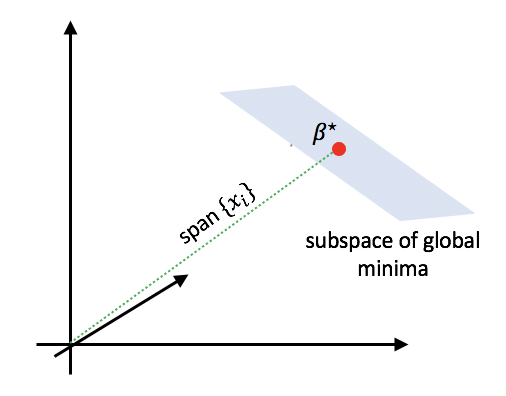
\includegraphics[width=.35\linewidth]{figures/subspace-global-min.png}
\caption{Visualization of proof intuition for Theorem~\ref{lec13:thm:linear-main}. The solution $\beta^\star$ is the projection of the origin onto the subspace of global minima.}
\label{lec13:fig:1}
\end{figure}

\begin{proof}
We first show via induction that $\beta^t \in \text{span}\l\{ x\sp{1}, \dots,x\sp{n} \r\}$ for all $t$. For the induction base case, note that $\beta^0 = 0 \in \text{span}\l\{ x\sp{1}, \dots,x\sp{n} \r\}$. Now suppose $\beta^{t-1} \in \text{span}\l\{ x\sp{1}, \dots,x\sp{n} \r\}$. Recall that $\beta^t = \beta^{t-1} - \eta \nabla \hatL(\beta^{t-1})$. Since left-multiplying any vector by $X^\top$ amounts to taking a linear combination of the rows of $X$, it follows that $\eta \nabla \hatL(\beta^{t-1}) = \eta X^\top(X\beta^{t-1} - y) \in \text{span}\l\{ x\sp{1}, \dots,x\sp{n} \r\}$, and so $\beta^t = \beta^{t-1} - \eta \nabla \hatL(\beta^{t-1}) \in \text{span}\l\{ x\sp{1}, \dots,x\sp{n} \r\}$. This proves the induction step.

Next, we show that $\hat \beta \in \text{span}\l\{ x\sp{1}, \dots,x\sp{n} \r\}$ and $\hatL(\hat \beta) = 0$ implies $\hat \beta = \beta^\star$. By definition, $\hat \beta \in \text{span}\l\{ x\sp{1}, \dots,x\sp{n} \r\}$ implies $\hat \beta = X^\top v$ for some $v \in \bbR^n$. Since $\hatL(\hat \beta) = 0$, we have $0 = X\hat \beta - y = X X^\top v - y$. This implies $v = (X X^\top)^{-1}y$, and so $\hat \beta = X^\top v = X^\top (X X^\top)^{-1} y = X^+ y = \hat \beta^\star$.
\end{proof}

\sec{Algorithmic regularization in non-linear models}
We give an example of algorithmic regularization in a non-convex version of the overparametrized linear regression task considered in the previous section.

Take $X$ and $y$ as defined in Section~\ref{lec13:sec:olr}. This time, our goal is to find a weight vector that minimizes our empirical loss function
\begin{equation}
\hatL(\beta) := \frac{1}{4n}\sum_{i=1}^n \left(y\sp{i} - f_\beta(x\sp{i})\right)^2,
\end{equation}
where $f_\beta(x):= \langle \beta \odot \beta, x\rangle$. (The operation $\odot$ denotes the Hadamard product: for $u,v \in \bbR^d$, $u \odot v \in \bbR^d$ is defined by $(u \odot v)_i := u_i v_i$ for $i = 1, \dots, d$.)

We assume $x\sp{1},...,x\sp{n} \iid \cN(0,I_{d \times d})$ and $y\sp{i} = f_{\beta^\star}(x\sp{i})$, where the ground truth vector $\beta^\star$ is $r$-sparse (i.e. $\|\beta^\star\|_0 = r$). For simplicity, we assume $\beta_i^\star = \mathbf{1} \{i \in S\}$ for some $S \subset [d]$ such that $|S| = r$. We again analyze the overparametrized setting, where this time $n \ll d$ but also $n \geq \widetilde \Omega(r^2)$.

\subsec{Main results of algorithmic regularization}
Note that while $f_\beta$ is still linear over $x$, our loss is no longer convex over $\beta$. (To see this, suppose $\beta \neq 0$ is a global minimizer. Then we have $\hatL(0) > \hatL(\beta) = \hatL(-\beta)$.) Thus, the effect of algorithmic regularization induced by gradient descent will be much different from the overparametrized linear regression setting. 

In the previous setting of linear regression, solutions with low $\ell_2$ norm are desirable as they tend to generalize well. In the present setting, we know our ground-truth parameter $\beta^\star$ is sparse. Thus, we want to learn a sparse solution $\hat \beta$, avoiding non-sparse solutions that may not generalize well. One approach to finding sparse solutions, called \textit{lasso regression}, is to minimize the $\ell_1$-regularized proxy loss
\begin{equation}
\sum_{i=1}^n \left(\langle \theta, x\sp{i} \rangle - y\sp{i} \right)^2 + \lambda \| \theta \|_1
\end{equation}
with respect to $\theta$, where $\theta = \beta \odot \beta$. However, it turns out that we can equivalently learn a sparse solution by running gradient descent from a suitable initialization on the original \textit{unregularized} loss.

To be specific, let $\beta^0=\alpha \mathbf{1} \in \R^d$ be the initialization where $\alpha$ is a small positive number. The update rule of gradient descent algorithm is given by $\beta^{t+1}=\beta^t-\eta\nabla \hatL(\beta^{t}).$ The next theorem shows that when $n=\widetilde{\Omega}(r^2)$, gradient descent on $\hatL(\beta)$ converges to $\beta^\star.$

\begin{theorem}\label{lec13:thm:non-linear-main}
Let $c$ be a sufficiently large universal constant. Suppose $n\ge cr^2\log^2(d)$ and $\alpha\le 1 / d^c$, then when $\dfrac{\log(d/\alpha)}{\eta}\lesssim T\lesssim \dfrac{1}{\eta\sqrt{d\alpha}},$ we have
\begin{equation}\label{lec13:eqn:non-linear-main}
    \l\|\beta^\top\odot\beta^\top-\beta^\star\odot\beta^\star \r\|_2^2\le O \l( \alpha\sqrt{d} \r).
\end{equation}

(Here, $T$ indexes the gradient descent steps.)
\end{theorem}

We make several remarks about Theorem~\ref{lec13:thm:non-linear-main} before presenting the proof.

\begin{remark}
In this problem we do not use $\beta^0=0$ as the initialization point because $\beta=0$ is a critical point, that is, $\nabla\hatL(0)=0$. Note that the lower bound on $T$ depends logarithimically on $1/\alpha$, so we can take $\alpha$ to be a small inverse polynomial on $d$ and the lower bound won't change much. Also, the upper bound depends polynomially on $1/\alpha$ (which is considered very big when $c$ is sufficiently large), so we do not need to use early stopping in a serious way.
\end{remark}

\begin{remark}
Theorem~\ref{lec13:thm:non-linear-main} is a simplified version of Theorem 1.1 in \cite{li2018algorithmic}.
\end{remark}

\begin{remark}
$\hatL(\beta)$ has many global minima. To see this, observe that the number of parameters is $d$ and the number of constraints to fit all the examples is $O(n)$ because there are only $n$ examples. Recall that for overparameterized model we have $d\gg n$; consequently, there exists many global minima of $\hatL(\beta)$.
\end{remark}

\begin{remark}
$\beta^\star$ is the min-norm solution in this case. That is,
    \begin{align}\label{lec13:eqn:opt}
        \beta^\star=\argmin \|\beta\|_2^2\qquad \text{s.t. }\hatL(\beta)=0.
    \end{align}
    Informally, this is because we can view $\beta\odot \beta$ as a vector $\theta\in \R^{d}$, which leads to $\|\beta\|_2^2 =\|\theta\|_1.$ Then in the $\theta$ space (and with a little abuse of notation), the optimization problem~\eqref{lec13:eqn:opt} becomes
    \begin{align}\label{lec13:eqn:opt-theta}
        \theta^\star=\argmin \|\theta\|_1 \qquad \text{s.t. }\hatL(\theta)=0,
    \end{align}
    which is a lasso regression, whose solution is sparse.
\end{remark}

\begin{remark}    
In this non-linear case and the linear case before, gradient descent with small initialization converges to minimum $\ell_2$-norm solution. Similarly, in the NTK regime, gradient descent converges to a solution that is very close to the initialization. Therefore, it seems conceivable that GD generally prefers global minima nearest to the initialization. However, we do not have a general theorem for this phenomenon (and the instructor also believes that this is not universally true without other conditions). 
\end{remark}

\subsec{Ground work for proof and the restricted isometry property}\label{lec13:sec:rip}

In this section we prepare the ground work for the proof of Theorem~\ref{lec13:thm:non-linear-main}.

We start by showing several basic properties about $\hatL(\beta)$. Note that for any fixed vector $v\in\R^{d}$ and $x\in \R^{d}$, when $x$ is drawn from $\cN(0,I)$, we have
\begin{equation}\label{lec13:eqn:gaussian-product}
    \Exp \l[\langle x, v\rangle^2 \r]=\Exp \l[ v^\top xx^\top v \r]=v^\top\Exp \l[ xx^\top \r]v=\|v\|_2^2.
\end{equation}

It follows that 
\begin{align}
    L(\beta)&=\frac{1}{4}\Exp_{x\sim \cN(0,I)} \l[(y-\langle \beta\odot\beta,x\rangle^2 \r] \\
    &=\frac{1}{4}\Exp_{x\sim \cN(0,I)} \l[\langle \beta^\star\odot\beta^\star-\beta\odot\beta,x\rangle^2 \r] &\text{(by definition of $y$)} \\
    &=\frac{1}{4} \l\| \beta^\star\odot\beta^\star-\beta\odot\beta \r\|_2^2.\label{lec13:eqn:loss-form} &\text{(by \eqref{lec13:eqn:gaussian-product})}
\end{align}
Note that \eqref{lec13:eqn:loss-form} is the metric that we use to characterize how close $\beta$ is to the ground-truch parameter $\beta^\star$ (see \eqref{lec13:eqn:non-linear-main}).

In the following lemma we show that $\hatL(\beta) \approx L(\beta)$ by uniform convergence. Generally speaking, uniform convergence of the loss function for all $\beta$ requires $n\ge \Omega(d)$ samples, so in our setting (where $n\ll d$) $\hatL(\beta) \approx L(\beta)$ does not always hold. However, since we assume $\beta^\star$ is sparse, the analysis only requires uniform convergence for sparse vectors.

\begin{lemma}\label{lec13:lem:RIP}
Assume $n\ge \widetilde\Omega(r^2)$. With high probability over the randomness in $x^{(1)},\cdots,x^{(n)}$, $\forall v$ such that $\|v\|_0\le r$ we have
\begin{equation}\label{lec13:eqn:RIP}
(1-\delta)\|v\|_2^2\le \frac{1}{n}\sum_{i=1}^{n}\langle v,x^{(i)}\rangle^2\le (1+\delta)\|v\|_2^2.
\end{equation}
\end{lemma}

Lemma~\ref{lec13:lem:RIP} is a special case of Lemma 2.2 in \cite{li2018algorithmic} so the proof is omitted here. We say the set $\l\{ x^{(1)},\cdots,x^{(n)} \r\}$ (or $X=[x^{(1)},\cdots,x^{(n)}]$) satisfies $(r,\delta)$\textit{-RIP condition} (\textit{restricted isometric property}) if \eqref{lec13:eqn:RIP} holds.

By algebraic manipulation, \eqref{lec13:eqn:RIP} is equivalent to 
\begin{align}\label{lec13:eqn:RIP-2}
(1-\delta)\|v\|_2^2\le v^\top \left(\frac{1}{n}\sum_{i=1}^{n}x^{(i)}(x^{(i)})^\top\right)v\le (1+\delta)\|v\|_2^2.
\end{align}
In other words, from the point of view of a sparse vector $v$ we have $\sum_{i=1}^{n}x^{(i)}(x^{(i)})^\top\approx I$. (Note however that $\sum_{i=1}^{n}x^{(i)}(x^{(i)})^\top$ is not close to $I_{d\times d}$ in other notions of closeness. For example, $\sum_{i=1}^{n}x^{(i)}(x^{(i)})^\top$ is not close to $I_{d\times d}$ in spectral norm. Another way to see this is that $\sum_{i=1}^{n}x^{(i)}(x^{(i)})^\top$ is a $d \times d$ matrix but only has rank $n \ll d$.)

As a result, with the RIP condition we have $\hatL(\beta)\approx L(\beta)$ if $\beta$ is sparse. With more tools we can also get $\nabla \hatL(\beta)\approx \nabla L(\beta)$. Let us define the set $S_r=\{\beta:\|\beta\|_0\le O(r)\}$, the set where we have uniform convergence of $\hatL$ and $\nabla \hatL$. Informally, as long as we are in the set $S_r$, $\hatL$ and $\nabla\hatL$ have similar behavior to their population counterparts. (Note, on the other hand, that there exists a dense $\beta\not\in S_r$ such that $\hatL(\beta)=0$ but $L(\beta)\gg 0.$)

The RIP condition also gives us the following lemma which will be needed for the proof of Theorem \ref{lec13:thm:non-linear-main}.

\begin{lemma}\label{lec14:lem:rip}
    Suppose $x^{(1)}, x^{(2)}, \dots x^{(n)}$ satisfy the $(r, \delta)$-RIP condition. Then, $\forall v, w$ such that $\Norm{v}_{0} \leq r$ and $\Norm{w}_{0} \leq r$, we have that
    \begin{align}
        \left| \frac{1}{n} \sum_{i=1}^{n} \langle x^{(i)}, v \rangle \langle x^{(i)}, w \rangle  - \langle v, w \rangle \right| &= \left|  v^{T} \l(\frac{1}{n} \sum_{i=1}^{n}  x^{(i)} (x^{(i)})^\top \r)  w  - \langle v, w \rangle \right| \\
        &\leq 4 \delta \Norm{v}_{2} \cdot \Norm{w}_{2}.
    \end{align} 
\end{lemma}

\tnotelong{To add proof of this lemma in the future.}
\begin{corollary}\label{lec14:cor:rip}
    Taking $w = e_1, \dots, e_d$ in Lemma~\ref{lec14:lem:rip}, we can conclude that
    \begin{align}
        \Norm{ \frac{1}{n} \sum_{i=1}^n \langle x^{(i)}, v\rangle x^{(i)} - v }_\infty &= \Norm{ \l(\frac{1}{n} \sum_{i=1}^n x^{(i)}(x^{(i)})^\top \r)v - v }_\infty \\
        &\leq 4\delta \Norm{v}_2.
    \end{align}
\end{corollary}

\subsec{Warm up: Gradient descent on population loss}

The main intuition for proving Theorem~\ref{lec13:thm:non-linear-main} is to leverage the uniform convergence when $\beta$ belongs to the set $S_r$ (see Figure~\ref{lec13:fig:uc-sr}). Note that the initialization $\beta^0$ is not exactly $r$-sparse, but taking $\alpha$ to be sufficiently small, $\beta^0$ is approximately $0$-sparse. The proof is decomposed into the following steps:

\begin{enumerate}
    \item Gradient descent on $L(\beta)$ converges to $\beta^\star$ without leaving $S_r$, and
    \item Gradient descent on $\hatL(\beta)$ is similar to gradient descent on $L(\beta)$ inside $S_r$.
\end{enumerate}

Combining the two steps we can show that gradient descent on $\hatL(\beta)$ does not leave $S_r$ and converges to $\beta^\star.$

\begin{figure}
\centering
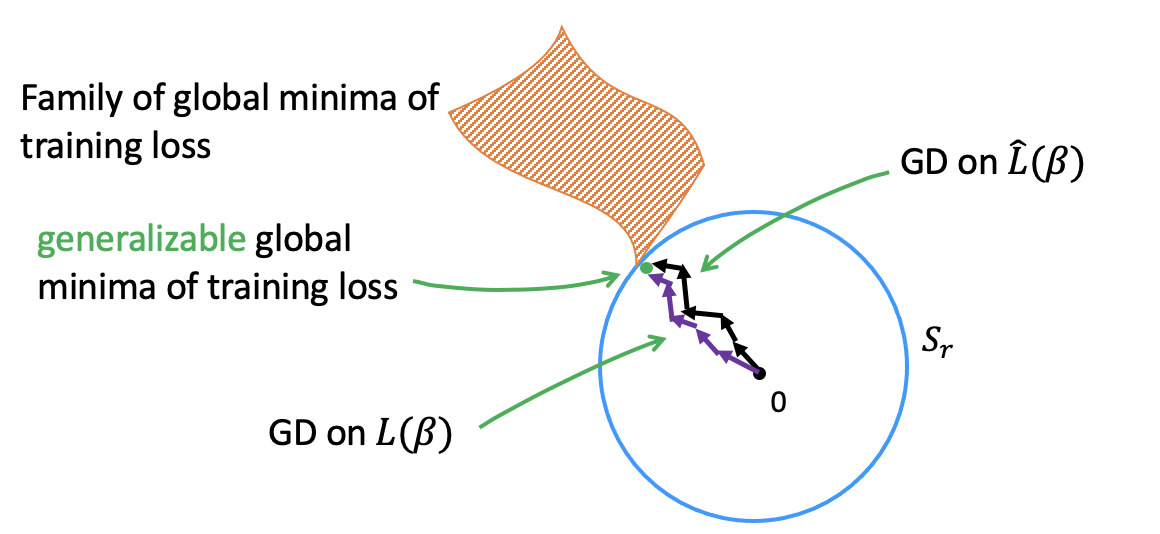
\includegraphics[width=.7\linewidth]{figures/uc-sr.png}
\caption{Visualization of proof intuition for Theorem~\ref{lec13:thm:non-linear-main}.}
\label{lec13:fig:uc-sr}
\end{figure}

As a warm up, we prove the following theorem for gradient descent on $L(\beta).$
\begin{theorem}
For sufficiently small $\eta$, gradient descent on $L(\beta)$ converges to $\beta^\star$ in $\Theta\left(\dfrac{\log (1/ (\epsilon\alpha) )}{\eta}\right)$ iteration with $\epsilon$-error in $\ell_2$-distance.
\end{theorem}

\begin{proof}

Since
\begin{equation}
\nabla L(\beta) = (\beta\odot \beta-\beta^\star\odot\beta^\star)\odot\beta,
\end{equation}

the gradient descent step is
\begin{equation}
\beta^{t+1} = \beta^t - \eta (\beta^t \odot \beta^t -\beta^\star \odot \beta^\star)\odot\beta^t.
\end{equation}

Recall that $\beta^\star=\mathbf{1} \{i \in S \}$ and $\beta^0=\alpha \mathbf{1}$, and the update rule above decouples across the coordinates of $\beta^t$. Thus, we only need to show that $| \beta_i^\star - \beta^t | \leq \epsilon$ for the number of iterations stated in the Theorem.

\underline{Case 1: $i\in S$.} For $i \in S$, the update rule for coordinate $i$ is
\begin{align}
\beta_i^{t+1} &= \beta_i^t - \eta (\beta_i^t \cdot \beta_i^t - 1 \cdot 1) \cdot\beta_i^t \\ 
&= \beta_i^t - \eta \l[ \left(\beta_i^t\right)^2 - 1 \r] \beta_i^t.
\end{align}

Consider the following two cases:

\begin{itemize}
\item If $\beta_i^t\le 1/2$, we have
\begin{align}
\beta_i^{t+1}&=\beta_i^{t} \l[ 1+\eta \l(1- \l(\beta_i^t \r)^2 \r) \r] \\
&\ge \beta_i^t \l( 1+\frac{3}{4}\eta \r).
\end{align}

Consequently, $\beta_i^{t+1}$ grow exponentially, and it takes $\Theta\left(\dfrac{\log (1/\alpha)}{\eta}\right)$ iterations for $\beta_i^t$ to grow from $\alpha$ to at least $1/2.$\footnote{This is because $(1+\eta)^{1/\eta}\approx e$, so $(1+\eta)^{c/\eta}\approx e^{c}.$} This will bring us into the second case.
    
\item if $\beta_i^t\ge 1/2$, we have
\begin{align}
1-\beta_i^{t+1}&=1-\beta_i^t+\eta \l[ \l(\beta_i^t \r)^2-1 \r] \beta_i^t\\
&=1-\beta_i^{t}-\eta \l( 1-\beta_i^t \r) \l(1+\beta_i^t \r)\beta_i^t\\
&\le 1-\beta_i^t-\eta \l( 1-\beta_i^t \r)\beta_i^t &\text{(because $1+\beta_i^t\ge 1$)} \\
&= \l(1-\beta_i^t \r) \l( 1-\eta \beta_i^t \r) \\
&\le \l( 1-\beta_i^t \r) \l(1-\eta/2 \r). &\text{(because $\beta_i^t\ge 1/2$)}
\end{align}

Therefore it takes $\Theta\left(\dfrac{\log (1/\epsilon)}{\eta}\right)$ iterations to achieve $1-\beta_i^t\le \epsilon.$
\end{itemize}

\underline{Case 2: $i \notin S$.} For all $i \notin S$, we claim (informally) that it is sufficient to show that when $t \leq 1 / (10 \eta \alpha^{2})$, $\beta_{i}^{t} \leq 2\alpha$. This is because when $i \notin S$, $\beta_{i}$ stays small and will take many iterations before it even gets to $2\alpha$, which is close to $0$ since $\alpha$ is chosen to be small.

For a coordinate $i\notin S$, the gradient descent update for this problem becomes
\begin{align}
    \beta_i^{t+1} &= \left[ \beta^{t} - \eta (\beta^{t} \odot \beta^{t} - \beta^\star \odot \beta^\star) \odot \beta^{t} \right]_i \\
    &= \beta_i^{t} - \eta (\beta_i^{t} \cdot \beta_i^{t}) \cdot \beta_i^{t} & (\text{since } \beta_{i}^\star = 0 \ \forall i \notin S) \\
    &= \beta_i^{t} - \eta (\beta_i^{t})^{3}.
\end{align}

Since our initialization $\beta^{0}$ was small, the update to these coordinates will be even smaller because $(\beta_{i}^{t})^{3}$ is small. We can prove the desired claim using strong induction. Suppose $\beta_{i}^{s} \leq 2\alpha$ for all $s \leq t$ and $i \notin S$, and that $t+1 \leq 1 / (10\eta \alpha^{2})$. Then, for all $s \leq t$,
\begin{align}
\beta_{i}^{s+1} %&= \beta^{s}_{i} - \eta (\beta_{i}^{s})^{3} \\
    &= (1 - \eta (\beta_{i}^{s})^{2})\beta_{i}^{s} \\
    &\leq (1 + \eta (\beta_{i}^{s})^{2}) \beta_{i}^{s} \\
    &\leq (1 + 4\eta \alpha^{2}) \beta_{i}^{s}. & (\text{since } \beta_{i}^{s} \leq 2\alpha)
\end{align}

With strong induction, we can repeatedly apply this gradient update starting from $t=0$ to obtain
\begin{align}
    \beta_{i}^{t+1} &\leq \beta_{0} \cdot (1 + 4 \eta \alpha^{2})^t \\
    &\leq \beta_{0} ( 1 + 4 \eta \alpha^{2})^{\frac{1}{10 \eta \alpha^{2} }} \\
    &\leq \beta_{0} \exp \bigg(\frac{4\eta \alpha^{2}}{10 \eta \alpha^{2}} \bigg) \\
    &=  \beta_{0} \cdot e^{2/5} \\
    &\leq 2 \alpha,
 \end{align}
 which completes the inductive proof of the claim.

\end{proof}
	% reset section counter
%\setcounter{section}{0}

%\metadata{lecture ID}{Your names}{date}
\metadata{14}{Roshni Sahoo and Sarah Wu}{Mar 3rd, 2021}

\subsec{Proof of main result: gradient descent on empirical loss}

Analyzing gradient descsent on the empirical risk $\empL$ is more complicated than analyzing gradient descent on the population risk, so we focus on the case when $\beta^\star$ is $1$-sparse, i.e. $r=1$. (When $r>1$, the main idea is the same but requires some more advanced analysis techniques.) 

Note that in our setup, i.e. when $x^{(1)} \ldots x^{(n)} \iid \mathcal{N}(0, I_{d\times d})$ and when $n\geq \widetilde{\Omega}(r/\delta^2)$, with high probability the data satisfy the $(r, \delta)$-RIP condition. It follows that when $r=1$ and $\delta = \tilO(1/\sqrt{n})$, the data are $(1, \delta)$-RIP. This will allow us to use the lemmas involving the RIP condition for the proof.

We restate the case of $r=1$ in the following theorem.
 
\begin{theorem} \label{lec14:thm:main}
Suppose $\eta \geq \widetilde{\Omega}(1).$ Then, gradient descent on $\empL$ with $t = \Theta \l(\frac{\alpha \log (1/\delta)}{\eta}\r)$ steps satisfies 
\begin{equation}
\Norm{\beta^{t} \odot \beta^{t} - \beta^\star \odot \beta^\star}_{2}^{2} \leq \tilO\l(\frac{1}{\sqrt{n}}\r).
\end{equation} 
\end{theorem}

\begin{remark}
Note that Theorem~\ref{lec14:thm:main} is a slightly weaker version of Theorem~\ref{lec13:thm:non-linear-main} for $r=1$, since the bound on the RHS depends on the number of examples and not the initialization $\alpha$. In Theorem~\ref{lec13:thm:non-linear-main}, we could take $\alpha$ as small as we like to drive the bound to zero; we cannot do this for Theorem~\ref{lec14:thm:main}.
\end{remark}

We proceed to prove Theorem~\ref{lec14:thm:main} with the follow steps:
\begin{enumerate}
\item Computing the gradient update $\nabla \empL$,
\item Dynamics analysis of noise $\zeta_t$, 
\item Dynamics analysis of signal $r_t$, and
\item Putting it all together.
\end{enumerate}

\underline{Computing the gradient update $\nabla \empL$}

WLOG, assume that $\beta^\star = e_{1}.$ We can decompose the gradient descent iterate $\beta^{t}$ as
\begin{equation}
    \beta^{t} = r_{t} \cdot e_{1} + \zeta_{t},
\end{equation}
where $\zeta_t \perp e_1$. The idea is to prove convergence to $\beta^\star$ by showing that (i) $r_{t} \rightarrow 1$ as $t \rightarrow \infty$, and (ii) $\norm{\zeta_{t}}_{\infty} \leq O(\alpha)$ for $t \leq \tilO\big(1/\eta).$ In other words, the \textit{signal} $r_{t}$ converges quickly to $1$ while the \textit{noise} $\zeta_t$ remains small for some number of initial iterations. One may be concerned that it is possible for the noise to amplify after many iterations, but we will not have to worry about this scenario if we can guarantee that $\beta^{t}$ converges to $\beta^\star$ first.

We can compute the gradient of $\empLt$ as follows. Since $y\sp{i} = \langle \beta^\star \odot \beta^\star, x\sp{i} \rangle$ and $\beta^{t} = r_{t}e_{1} + \zeta_{t} = r_{t}\beta^\star + \zeta_{t}$,
\begin{align}
    \nabla \empLt &= \frac{1}{n} \sum_{i=1}^{n} (\langle \beta^{t} \odot \beta^{t}, x\sp{i} \rangle - y\sp{i} ) x\sp{i} \odot \beta^{t} \\
    &= \frac{1}{n} \sum_{i=1}^{n} ( \langle \beta^{t} \odot \beta^{t} - \beta^\star \odot \beta^\star, x\sp{i} \rangle ) x\sp{i} \odot \beta^{t} \\
    &= \frac{1}{n} \sum_{i=1}^{n} \langle r_{t}^{2} \beta^\star \odot \beta^\star + \zeta_{t} \odot \zeta_{t} - \beta^\star \odot \beta^\star, x\sp{i}  \rangle x\sp{i} \odot \beta^{t} \\
    &= \underbrace{\frac{1}{n} \sum_{i=1}^{n} \Big\langle \big(r_{t}^{2} - 1\big) \beta^\star \odot \beta^\star + \zeta_{t} \odot \zeta_{t}, x\sp{i}  \Big\rangle x\sp{i}}_{m_t} \odot \beta^{t}.
\end{align}

To simplify the analysis, we can rearrange some of the terms that are part of the gradient. Define $m_{t} $ such that $\nabla \empLt = m_{t} \odot \beta^{t}.$ Also, let $X = \frac{1}{n} \sum_{i=1}^{n} x\sp{i}(x\sp{i})^\top.$ Then,
\begin{align}
    m_{t} &= \frac{1}{n} \sum_{i=1}^{n} \Big\langle \big(r_{t}^{2} - 1\big) \beta^\star \odot \beta^\star + \zeta_{t} \odot \zeta_{t}, \ x\sp{i}  \Big\rangle \ x\sp{i} \\
    &= \l( \frac{1}{n} \sum_{i=1}^{n} x\sp{i}\big(x\sp{i}\big)^\top \r) \l(r_{t}^{2} - 1\r) \cdot \l(\beta^\star \odot \beta^\star\r) + \l( \frac{1}{n} \sum_{i=1}^{n} x\sp{i}(x\sp{i})^\top \r) \l(\zeta_{t} \odot \zeta_{t}\r) \\
    &= \underbrace{X \big(r_{t}^{2} - 1\big) \cdot \big(\beta^\star \odot \beta^\star\big)}_{\text{part of } u_t} + \underbrace{X \big(\zeta_{t} \odot \zeta_{t}\big)}_{v_t}.
\end{align}

Now, define $u_{t} := (r_{t}^{2} - 1) (\beta^\star \odot \beta^\star) - X (r_{t}^{2} - 1) (\beta_{*} \odot \beta_{*})$ and $v_{t} := X \big(\beta_{t} \odot \beta_{t}\big)$. Then we can rewrite the gradient as

\begin{equation}
    \nabla \empLt = m_{t} \odot \beta^{t} = [(r_{t}^{2} -1) \beta^\star \odot \beta^\star - u_{t} + v_{t}] \odot \beta_{t}. \label{lec14:eqn:emp-gradient}
\end{equation}

Our goal is to show that both $u_t$ and $v_t$ are small, so that $\nabla \empLt$ is close to its population version $\nabla L(\beta^t)$. Observe that $X$ appears in both $u_{t}$ and $v_{t}$. This matrix is challenging to deal with mathematically because it does not have full rank (because $n < d$). Instead, we rely on the RIP condition to reason about the behavior of $X$: the idea is that $X$ behaves like the identity for sparse vector multiplication. Applying Corollary~\ref{lec14:cor:rip}, we can bound $\Norm{u_{t}}_{\infty}$ as
\begin{equation} \label{lec14:eqn:u-inf-norm}
    \Norm{u_{t}}_{\infty} \leq 4\delta \Norm{(r_t^2 - 1)  \beta^\star \odot \beta^\star }_{2} 
    \leq 4\delta ||\beta^\star \odot \beta^\star||_{2} \leq 4\delta.
\end{equation}

(In the second inequality, we assume that $|r_t| < 1$. We can do this because $r_t$ starts out at $\alpha$ which is small; if $r_t \geq 1$, then we are already in the regime where gradient descent has converged.) We can bound $\Norm{v_{t}}_{\infty}$ in a similar manner: since Corollary~\ref{lec14:cor:rip} implies $\Norm{v_t - \zeta_t \odot \zeta_t}_\infty \leq 4\delta \Norm{\zeta_{t} \odot \zeta_{t}}_{2}$,
\begin{align}
    \Norm{v_{t}}_{\infty} &\leq \Norm{\zeta_{t} \odot \zeta_{t}}_{\infty} + 4\delta \Norm{\zeta_{t} \odot \zeta_{t}}_{2} &(\text{by the triangle inequality}) \\
    &\leq \Norm{\zeta_{t}}_{\infty}^{2} + 4\delta \Norm{\zeta_{t} \odot \zeta_{t}}_{1} &(\text{since } \zeta_t \text{ very small}) \\
    &= \Norm{\zeta_{t}}_{\infty}^{2} + 4\delta \Norm{\zeta_{t}}_{2}^{2}. \label{lec14:eqn:v-inf-norm}
\end{align}

Note that the size of $v_t$ depends on the size of the noise $\zeta_t$. Thus, by bounding $\zeta_t$ (e.g. with a small initialization), we can ensure that $v_t$ is also small. (Ensuring bounds on $u_t$ is more difficult because it depends only on $\delta$.) In the next two subsections, we analyze the growth of $\zeta_t$ and $r_t$.

\underline{Dynamics analysis of $\zeta_t$}

First, we analyze the dynamics of the noise $\zeta_t$, which we want to ensure does not grow too fast.

\begin{lemma} \label{lec14:lem:dynamics_noise}
    For all $t\leq 1 / (c\eta\delta)$ with sufficiently large constant $c$, we have
    \begin{equation} \label{lec14:eqn:dynamics_noise}
        \Norm{\zeta_t}_\infty \leq 2\alpha, \quad \quad \Norm{\zeta_t}_2^2 \leq \frac{1}{2}, \quad \quad \text{and} \quad \Norm{\zeta_{t+1}}_\infty \leq \big(1 + O(\eta\delta)\big) \Norm{\zeta_t}_\infty.
    \end{equation}
\end{lemma}
Note that this result is weaker than what we were able to show for the population gradient (exponential growth with a small fixed rate), but we will ultimately show that the growth of the signal will be even faster.

\begin{proof}
Recall that the empirical gradient \eqref{lec14:eqn:emp-gradient} is $\nabla \hat{L}(\beta) = \big[(r_{t}^{2} - 1) \beta^\star \odot \beta^\star - u_{t} + v_{t} \big] \odot \beta^{t}$. Hence, the gradient update to $\beta^{t}$ is

\begin{align}
\beta^{t+1} &= \beta^{t} - \eta \l[\l(r_{t}^{2} - 1\r) \beta^\star \odot \beta^\star - u_{t} + v_{t} \r] \odot \beta^{t} \\
&= \underbrace{\beta^{t} - \eta \l(r_{t}^{2} - 1\r) \beta^\star  \odot \beta^\star \odot \beta^{t}}_{\text{GD update for population loss}} - \eta \l(- u_{t} + v_{t}\r) \odot \beta^{t}. \label{lec14:eqn:gd-update}
\end{align}
    
Recall that $\zeta_{t+1}$ is simply $\beta^{t+1}$ except for the first coordinate (where it has a zero instead of $r_{t+1}$), i.e. $\zeta_{t+1}$ is the projection of $\beta^{t+1}$ onto the subspace orthogonal to $e_1$. Hence,
\begin{align}
\zeta_{t+1} &= \l(I - e_{1} e_{1}^\top\r) \beta^{t+1} \\
&= \l(I - e_{1} e_{1}^\top\r) \cdot \beta^{t} - \eta \l(I - e_{1} e_{1}^\top\r) (v_{t} - u_{t}) \odot \beta^{t} &\text{(by \eqref{lec14:eqn:gd-update}, second term = 0)} \\
&= \zeta_{t} - \eta \l[\l(I - e_{1}e_{1}^{T}\r) (v_{t} - u_{t}) \odot \l(I - e_{1}e_{1}^{T}\r) \beta^{t}\r] &(\text{by distribution law for $\odot$}) \\
&= \zeta_t - \eta \underbrace{\l[ \l(I - e_{1}e_{1}^{T}\r) \l(v_t - u_t\r)\r]}_{\rho_t} \odot \zeta_t.
\end{align}
    
If we define $\rho_t$ such that $\zeta_{t+1} = \zeta_t - \eta \rho_t \odot \zeta_t$, then the growth of $\zeta_t$ is dictated by the size of $\rho_t$. We can bound this as
\begin{equation}
\Norm{\zeta_{t+1}}_{\infty} \leq (1 + \eta \Norm{\rho_{t}}_{\infty}) \Norm{\zeta_{t}}_{\infty}. \label{lec14:eqn:zeta-growth-bd}
\end{equation}

Now, we will prove the lemma by using strong induction on $t$. Suppose that the first two pieces of \eqref{lec14:eqn:dynamics_noise} hold for all iterations up to $t$. We can show that
\begin{align}
\Norm{\rho_{t}}_{\infty} &\leq \Norm{u_{t}}_{\infty} + \Norm{v_{t}}_{\infty}  \\
&\leq 4\delta + \Norm{\zeta_t}_{\infty}^{2} + 4\delta \Norm{\zeta_t}_{2}^{2} &(\text{by \eqref{lec14:eqn:u-inf-norm} and \eqref{lec14:eqn:v-inf-norm}}) \\
&\leq  4\delta + (2\alpha)^2 + 4\delta \cdot \frac{1}{2} &(\text{by the inductive hypothesis})\\
\label{lec14:eqn:diff-inf-norm}
&\leq 8\delta,
\end{align}
where the last step holds because we can take $\alpha$ to be arbitrarily small (e.g. $\alpha \leq \text{poly}(1/n) \leq O(\delta)$). Plugging this into \eqref{lec14:eqn:zeta-growth-bd}, we have
\begin{equation}
\Norm{\zeta_{t+1}}_\infty \leq (1 + 8\eta \delta) \Norm{\zeta_t}_{\infty} = \big(1 + O(\eta\delta)\big) \Norm{\zeta_t}_\infty,
\end{equation}
which proves the third piece of the lemma. Using this piece, we can show that
\begin{equation}
\Norm{\zeta_{t+1}}_{\infty} \leq \l(1 + 8 \eta \delta\r)^{t+1} \Norm{\zeta_{0}}_{\infty} \leq \big(1 + 8\eta \delta\big) ^{1/(c\eta \delta)} \cdot \alpha  \leq 2\alpha
\end{equation}
for a sufficiently large constant $c$, which proves the second piece. Finally, we show that
\begin{equation}
\Norm{\zeta_{t+1}}_{2}^2 \leq \big(1 + 8\eta \delta\big)^{t+1}\Norm{\zeta_{0}}_{2}^2 \leq \big(1 + 8\eta \delta)^{1/(c\eta \delta)} \cdot \alpha \sqrt{d} \leq \frac{1}{2},
\end{equation}
if $\alpha \leq \frac{1}{n^{O(1)}}$, which proves the first piece.

\end{proof}

\underline{Dynamics analysis of $r_t$}

Next, we analyze the dynamics of the signal $r_t$, which we want to show converges to 1.

\begin{lemma} \label{lec14:lem:dynamics_signal}
    For all $t\leq 1 / (c\eta\delta)$ with sufficiently large constant $c$, we have that
    \[ r_{t+1} = \big(1 + \eta\big( 1 - r_t^2 \big) \big) r_t + O\big(\eta\delta\big) r_t. \]
\end{lemma}
Note that the first term on the RHS is $r_{t+1}$ during gradient descent on the population loss, and the second term captures the error.

\begin{proof}
    Recall that the gradient descent update from the empirical gradient~\eqref{lec14:eqn:emp-gradient} is
    \begin{equation}
        \beta^{t+1} = \beta^t - \eta \big[\big(r_{t}^{2} -1\big) \beta^\star \odot \beta^\star - u_{t} + v_{t}\big] \odot \beta_{t}.
    \end{equation} 
    We have that
    \begin{align}
        r_{t+1} &= \big\langle \beta^{t+1}, e_1\big\rangle \\
        &= \big\langle \beta^t, e_1\big\rangle - \eta \big(r_{t}^{2} -1\big)\big\langle \beta^t, e_1\big\rangle - \eta \big\langle v_t-u_t, e_1\big\rangle \big\langle \beta^t, e_1 \big\rangle \\
        &= r_t - \eta \big(r_{t}^{2} -1\big) r_t - \eta \big\langle v_t-u_t, e_1\big\rangle r_t \\
        &= \Big(1 + \eta\big( 1 - r_t^2 \big) \Big) r_t + \eta \big\langle u_t-v_t, e_1\big\rangle r_t
    \end{align}
    so all we need to do is bound the second term as follows:
    \begin{align}
        |\eta \langle v_t - u_t, e_1\rangle r_t| &\leq \eta \cdot r_t \Norm{v_t-u_t}_\infty \\
        &\leq \eta \cdot r_t \cdot 8\delta &(\text{by \eqref{lec14:eqn:diff-inf-norm}}) \\
        &= O(\eta\delta) \cdot r_t.
    \end{align}
\end{proof}

\underline{Putting it all together}
Finally, we return to the proof of Theorem~\ref{lec14:thm:main}. By Lemma~\ref{lec14:lem:dynamics_signal}, we know that as long as $r_t \leq 1/2$ it will grow exponentially fast, since
\begin{equation}
    r_{t+1} \geq \Big(1 + \eta\big(1-r_t^2\big) - O(\eta\delta) \Big) \cdot r_t \geq \bigg(1 + \frac{\eta}{2}\bigg)\cdot r_t.
\end{equation} 
This implies that at some $t_0 = O\Big(\frac{\log (1/\alpha)}{\eta}\Big)$, we'll observe $r_{t_0} > 1/2$ for the first time. Consider what happens after this point.

\begin{itemize}
    \item When $1/2 < r_t \leq 1$, we have that
    \begin{align}
        1 - r_{t+1} &\leq 1 - r_t - \eta \big(1 - r_t^2\big) r_t + O(\eta\delta) \cdot r_t \\
        &\leq 1 - r_t - \frac{\eta \big(1 - r_t^2\big)}{2} + O(\eta\delta) \\
        &\leq 1 - r_t - \frac{\eta \big(1 - r_t\big)}{2} + O(\eta\delta) \\
        &= \bigg(1 - \frac{\eta}{2}\bigg) (1 - r_t) + O(\eta\delta).
    \end{align}
    Thus, we can achieve $1 - r_{t+1} \leq 2 \cdot \frac{O(n\delta)}{\eta/2} = O(\delta)$ in $\Theta\Big(\frac{\log(1/\delta)}{\eta}\Big)$ iterations.
    
    \item When $r_t > 1$, we can show in a similar manner that
    \begin{equation}
        r_{t+1} - 1 \leq (1 - \eta) (r_t - 1) + O(\eta\delta) \leq O(\delta),
    \end{equation} 
    implying that $r_t$ remains very close to 1 after the same order of iterations.
\end{itemize}

This completes the proof of Theorem~\ref{lec14:thm:main}, bounding the number of iterations needed for gradient descent on the empirical loss to converge to $\beta^*$.
\qed 

	% reset section counter
%\setcounter{section}{0}

%\metadata{lecture ID}{Your names}{date}
\metadata{17}{Jeff Z. HaoChen and Carrie Wu}{Mar 15th, 2021}

\sec{Algorithmic regularization for classification}

In this section, we will discuss algorithmic regularization for classification problem. In particular, we consider binary classification with logistic loss. Let $\{(x_i, y_i)\}_{i=1}^n$ be a separable dataset with $y_i\in \{\pm 1\}$, $x_i\in \R^d$. We have a linear model $h_w(x) = w^\top x$, and we minimize the empirical logistic loss 
\begin{align}
	\hatL (w) &= \frac{1}{n} \sum_{i=1}^{n} \ell(y_i h_w(x_i))\\
	&= \frac{1}{n} \sum_{i=1}^{n} \ell(y_i w^\top x_i),
\end{align}
where $\ell(t) = \log(1+\exp(-t))$ is the logistic loss.

In order to observe algorithmic regularization, we need to ensure that there exist multiple global minima for this setup. This is the case here: because the dataset is linearly separable, there exists some $w$ such that $y_i w^\top x_i > 0$ for all $i$. Clearly any $w'$ in a small neighborhood of $w$ also classifies all the data correctly; hence, there exists an infinite number of separating classifiers $\overline{w}$ with unit norm. For any of these $\overline{w}$, note that $\hatL(\alpha\overline{w}) \rightarrow 0$ as $\alpha \rightarrow \infty$, hence intuitively all of ``$\infty \overline{w}$'' classifiers are global minima.

Having shown the existence of multiple global minima, we now show that gradient descent will actually converge to the solution which maximizes the \textit{margin}. We first define the \textit{normalized margin} for a separating classifier $w$ as
\begin{align}
	\gamma(w) = \frac{\min_{i\in [n]} y_iw^\top x_i }{\|w\|_2}.
\end{align}
We call $\overline{\gamma} = \max_w \gamma(w)$ the \textit{max margin}. Now we are ready to state the theorem:

\begin{theorem}[\cite{soudry2018implicit}]
	Gradient descent with iterates $w_t$ converges to the direction of a max-margin solution:
	
	\begin{align}
		\gamma(w_t) \rightarrow \overline{\gamma} \quad  \text{as} \quad t \rightarrow \infty.
	\end{align}
	In other words, gradient descent on logistic loss is equivalent to the SVM.\footnote{This result is still very limited it only works without regularization, and one needs to run gradient descent for a long time before this convergence in direction happens. Also, SVM is not always the best possible solution.}
\end{theorem}

Here, we provide the intuition behind the proof. The proof of this theorem follows these steps:
\begin{enumerate}
	\item By standard convex optimization arguments, $\hatL (w_t) \rightarrow 0$ as $t\rightarrow \infty$.
	\item For sufficiently large $t$, $\|w_t\|_2 \rightarrow \infty$.
	\item For sufficiently large $t$, $w_t$ will separate the data (since the loss goes to 0).
	\item As $z \rightarrow \infty$, $l(z) = \log(1 + \exp (-z)) \approx \exp(-z)$ (i.e. logistic loss is similar to exponential loss). 
	\item When $\|w\|_2 = q $ is big, the loss $\hatL(w)$ mainly depends on supporting data $\{(x_i, y_i) : y_i\overline{w}^\top x_i = \gamma(w)\}$.
\end{enumerate}

To see the last bullet point: letting $\overline{w} = w / \|w\|_2$, we notice that 
\begin{align}
	\hatL &= \frac{1}{n} \sum_{i=1}^{n} \ell(y_i w^\top x_i)\\
	&\approx \frac{1}{n} \sum_{i=1}^{n} \exp\left(-qy_i \overline{w}^\top x_i\right) \label{lec17:eqn:reg-approx1} \\
	&\approx \frac{1}{n} \sum_{i=1}^{n} \exp\left(-qy_i \overline{w}^\top x_i\right) 1\left[y_i \overline{w}^\top x_i = \gamma(w)\right] \label{lec17:eqn:reg-approx2} \\
	&= \frac{1}{n} \sum_{i=1}^{n} \exp\left(-q\gamma(w) \right) 1\left[y_i \overline{w}^\top x_i = \gamma(w)\right]. \label{lec17:eqn:reg-approx3}
\end{align}
Here the first approximation~\eqref{lec17:eqn:reg-approx1} is because of the logistic loss vs. exponential loss approximation, while the second approximation~\eqref{lec17:eqn:reg-approx2} is because for any data $x_i, y_i$ that is not a support vector, i.e.
\begin{align}
	\overline{w}^\top x_i y_i \ge \gamma(w)+\epsilon,
\end{align}
for $\epsilon>0$, then
\begin{align}
	\exp(-qy_i\overline{w}^\top x_i) \le \exp(-q\gamma(w))\exp(-q\epsilon),
\end{align}
and as $q\rightarrow \infty$ the term $\exp(-q\epsilon)\rightarrow 0$, making such terms negligible.

In conclusion, minimizing the (approximate) loss~\eqref{lec17:eqn:reg-approx3} is (informally) equivalent to maximizing the margin. (Note that if you examine \eqref{lec17:eqn:reg-approx3}, there are actually two ways to make the loss small: maximizing the margin or making $q$ large. The rigorous proof shows that when $q$ is large, the margin is already very close to the max margin. These are technical details that we will not concern ourselves with.)

\sec{Stochasticity in algorithmic regularization}
Finally, we note that in general, when the loss has multiple global minima, any decisions we make about the optimization algorithm will make a difference. Another important source of algorithmic regularization (possibly the most important) comes from the \textit{stochasticity} in the stochastic gradient descent (SGD) algorithm, where the parameters are optimized by updates of the form
\begin{equation}
\theta_{t+1} = \theta_t - \eta(\nabla\hat{L}(\theta_t) + \xi_t),
\end{equation}

where $\xi_t$ is a random noise term, typically with $\E\left[\xi_t\right]=0$ so the noise will not affect the result too much. The variance of $\xi_t$ can sometimes be time-dependent: for example, $\xi_t$ could be dependent on the parameter $\theta_t$. 

In practice, it turns out that larger gradient noise can lead to better generalization performance, as long as the algorithm can optimize under such level of noise. The intuition behind this phenomenon is that SGD converges to a ``flat'' global minimum, i.e. one with small curvature and small noise covariance. On the other hand, if you have a ``sharp'' local/global minimum with a large amount of noise, SGD will not converge to it stably. There are a number of works on this topic~\cite{haochen2020shape,blanc2020implicit}, but a lot of questions in this space remained to be answered.

	
	\chapter{Data-dependent generalization bounds}
	% reset section counter
\setcounter{section}{0}

%\metadata{lecture ID}{Your names}{date}
\metadata{18}{Kaidi Cao, Ruocheng Wang}{Mar 17th, 2021}

% ===============================================

In this chapter, we discuss the Lipschitzness of models and why they seem to generalize better than arbitrary networks. To do so, we introduce a refined notion of uniform convergence that is data-dependent, and use it to derive a generalization bound for generalized margin. We end by introducing the \textit{all-layer margin}, a specific instance of generalized margin that captures model Lipschitzness, thus allowing us to use the data-dependent generalization bound.

\sec{Lipschitzness of models and generalization} \label{sec:all_layer_margin}
It has been found that the Lipschitzness of the model plays an important role in algorithmic regularization. As an illustration, note that the curvature (Hessian) of the loss function, the Lipschitzness of the model, and the noise level in SGD are all closely-related. To give a sense of the connections between them, suppose we have a model $f(x; \theta)$, a single example $(x, y)$, and a loss function $L(\theta) = \ell (f(x), y) = (f(x) - y)^2$. In this setup, we have the decomposition
\begin{align}
\nabla^2 L(\theta) = \underbrace{{\frac{\partial^2 \ell}{\partial f^2}}}_{\text{scalar}} \cdot \underbrace{\frac{\partial f}{\partial \theta}}_{\mathbb{R}^p} \cdot \underbrace{\frac{\partial f}{\partial \theta}^\top}_{\mathbb{R}^p} + \frac{\partial \ell}{\partial f} \cdot  \underbrace{\frac{\partial^2 f}{\partial \theta^2}}_{\mathbb{R}^{p\times p}}.
\end{align}

This decomposition is useful because it has been found empirically that the second term is relatively small. This implies that the Hessian is somewhat dominated by the first term. The first term, especially $\frac{\partial  f}{\partial \theta}$, relates to the Lipschitzness of the model with respect to the parameter. (There are similar connections between other quantities.)

Our algorithmic choices (e.g. SGD) seem to prefer Lipschitz models\footnote{By this we mean the Lipschitz constant of the model is small. Also, we are not distinguishing between the Lipschitz constant w.r.t to the input and that w.r.t. to the parameter because they are actually related (not covered in the lecture).}, which implies that such models generalize better. It remains to answer the question: \textbf{Why do Lipschitz models generalize better than arbitrary networks?} We want to theoretically analyze the relationship between Lipschitzness and generalization performance, and derive some generalization bounds w.r.t to the Lipschitzness of the models.

First, we note that the idea of using Lipschitzness to obtain generalization bounds is not new: it is the core of non-parametric statistics. However, such bounds suffer from the ``curse of dimensionality'', that is, the sample complexity grows exponentially as the data dimension $d$. Thus, using only Lipschitzness property is not enough to explain the generalization performance of neural networks: we need the help of parameterization. 

Consider a deep neural network $f(x) = \sigma(W_r\sigma(W_{r-1}\cdots \sigma(W_1x)))$ for binary classification. Recall, \cite{bartlett2017} showed that:
\begin{equation}
L(\theta) \leq \frac{R_S (\cF) }{\gamma},
\end{equation}
where $\gamma$ is the margin of the model, and $R_S (\cF)$ is some complexity that satisfies
\begin{equation}
R_S (\cF) \leq \underbrace{\l(\prod_{i=1}^r\|W_i\|_{\textup{op}} \r)}_{\text{relatively large}} \cdot \underbrace{\l( \sum_{i=1}^r\frac{\|W_i^\top\|^{2/3}_{2,1}}{\|W_i\|_{\textup{op}}^{2/3}}\r)^{3/2}}_{\text{relatively small}}.
\end{equation}
The first term is essentially the upper bound on the Lipschitzness of the model w.r.t. to the input over the entire space. 

The limitation of this bound is that if $\norm{W_i}_{\textup{op}} >1$, then it grows exponentially in depth. On the other hand, if $\norm{W_i}_{\textup{op}} < 1$, then the $f_\theta(x)$ is exponentially small. Thus, it is very hard to make the spectral norm small while keeping the margin large. In the typical case, we have
\begin{align}
    \norm{W_1x} &\approx \norm{W_1}_{\textup{op}}\norm{x}, \\
    \norm{\sigma(W_1x)} &\approx \frac{1}{\sqrt{2}}\norm{W_1}_{\textup{op}}\norm{x}.
\end{align}
(The second approximation comes from the heuristic that the ReLU function $\sigma$ will zero out about half of the entries.) Thus, heuristically the output shrinks by a factor of $\sqrt{2}$ when passing through each layer. To make the output $f(x)\approx \Theta(1)$, we need $\norm{W_i}_{\textup{op}}\approx \sqrt{2}$, which makes the generalization bound very large. 

The deeper cause to this problem is that $\prod_i \norm{W_i}_{\textup{op}}$ is a worst-case bound on the Lipschitzness of models, since it is data-independent and assumes that the input spans over the entire space. Thus one way to improve the bound is by replacing ``worse-case Lipschitzness'' with the Lipschitzness at the data points $x^{(1)}, \cdots, x^{(n)}$. This also allows us to estimate the Lipschitzness on the empirical data, and gives us a regularizer roughly in accordance with what SGD prefers.

We want to prove a bound of the form
\begin{equation}\label{lec18:eqn:data_dependent}
L(w)\leq \text{poly}(\text{Lipschitzness of $f_w$ on $x^{(1)}, \cdots, x^{(n)}$}, \text{norms of $W_i$'s}).
\end{equation}
The RHS of \eqref{lec18:eqn:data_dependent} can be used as an explicit regularizer in model training to improve the generalization performance. 

\sec{Proving data-dependent generalization bounds}
Before we prove a bound in the of form \eqref{lec18:eqn:data_dependent}, we first discuss why classical uniform convergence does not work. Note that the RHS of \eqref{lec18:eqn:data_dependent} is dependent on random variables $x^{(1)}, \cdots, x^{(n)}$. But typical bound of uniform convergence using Rademacher complexity is in the form
\begin{equation}
\forall f \in \cF,\quad L(f) \leq \text{comp}(\cF, n),
\end{equation}
where $\text{comp}$ is some complexity measure, or in the form
\begin{equation}
\forall f \in \cF, \quad L(f) \leq \text{comp}(f, n).
\end{equation}
The second bound can be achieved by defining $\cF_C= \{f: \text{comp}(f, n)\leq C\}$ first, applying the first type of bound for the class $\cF_C$, then performing a union bound over $C$. However, this approach does not work for obtaining a bound like the RHS of~\eqref{lec18:eqn:data_dependent} because the the corresponding hypothesis class is
\begin{equation}
\cF_C = \l\{f: \text{comp}(f, \{ (x\sp{i}, y\sp{i}) \}_{i=1}^n, n) \leq C \r\}.
\end{equation}
There are random variables in the definition of the hypothesis class, which is not allowed for Rademacher complexity. Hence, we cannot leverage such techniques directly.

To tackle this issue, we introduce a refined version of uniform convergence. Suppose we can decompose the complexity measure into the sum of a property related to each data point and the function we care about:
\begin{align}
\text{comp} \l(f, \{x^{(i)}, y^{(i)} \}_{i=1}^n, n \r) = \sum_{i=1}^n g((x^{(i)}, y^{(i)}), f).
\end{align}

We can define the \textit{augmented loss} as

\begin{align}
\Tilde{l} (f) = l(f) \cdot \bm{1} (g((x, y), f) \le C).
\end{align}

This means that we are changing the loss function to include the data-dependent term. An intuitive example can be found in Figure~\ref{lec18:fig:surrogate_loss}, where we have an empirical loss with very bizarre behavior, but only outside the low complexity region that we really care about. The augmented loss notices this and ``smooths out'' the irregularities outside the low complexity region by ignoring those terms.

\begin{figure}[htpb]
    \centering
    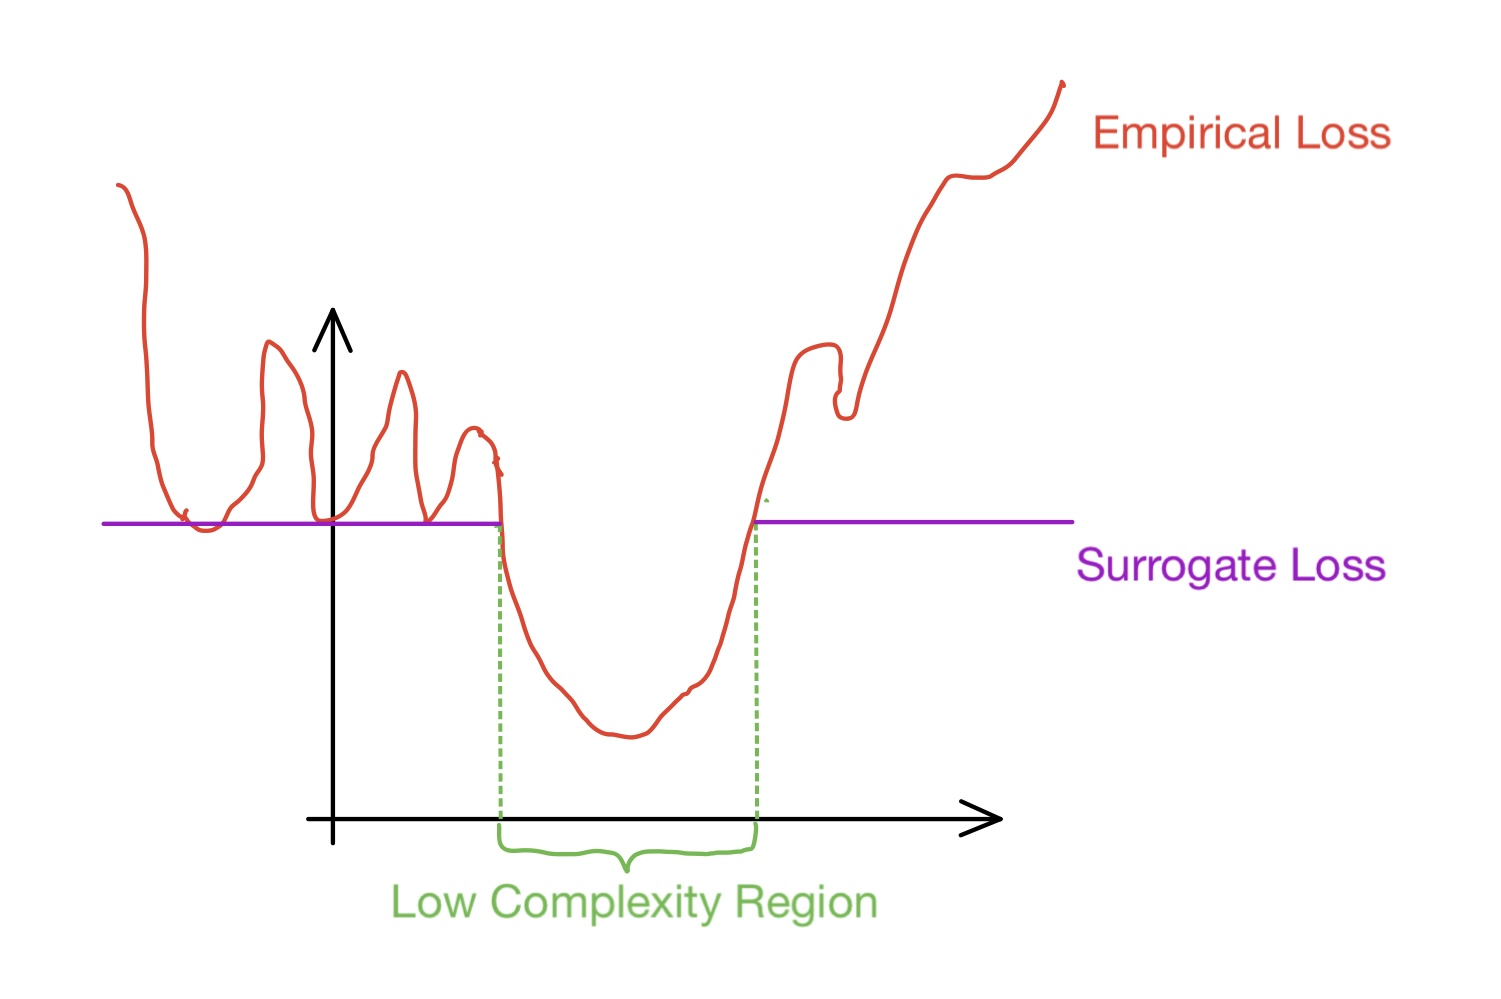
\includegraphics[width=0.7\textwidth]{figures/surrogate_loss.jpg}
    \caption{The empirical loss has bizarre behavior, but only outside the region of interest. The general idea is to define a surrogate loss and prove uniform convergence over the surrogate loss so as to avoid the bizarre behavior of the empirical loss.}
    \label{lec18:fig:surrogate_loss}
\end{figure}

The difficulty with taking this approach is that the low complexity region is random: if it was fixed, we could just zoom into that region and prove something directly by uniform convergence. We deal with this difficulty by defining a \textit{surrogate loss} which it could just be constant outside of the low complexity region. We may then apply uniform convergence over the entire space.

We have talked about the notion of surrogate losses before in this class. For example, the margin loss/ramp loss is a type of surrogate loss. There, we thought of using the surrogate loss to make the zero-one loss more continuous. Here, we use the surrogate loss to avoid dealing with the loss function in ``bad'' regions. Let us define a generalized version of margin loss:

\begin{definition}[Generalized margin]
Let $f : \R^d \mapsto \R$ be a classification model. We call $g_f(x, y)$ a \textit{generalized margin} if $g_f(x,y)$ satisfies
\begin{align}
    g_f(x, y) = \begin{cases} 0 &\text{if } f(x)\cdot y \le 0 \quad \text{(wrong prediction)}, \\  > 0 &\text{if } f(x)\cdot y > 0. \end{cases}
\end{align}
\end{definition}

Given this definition, we have the following lemma:
\begin{lemma}[Generalization bound for general margin]
\label{lec18:lem:generalizedmargin}
Suppose $g_f$ is a generalized margin. Let $G = \{ g_f : f \in \mathcal{F} \}$, and assume we have an $\epsilon$-covering of $G$ under the $\norm{\cdot}_\infty$ metric, $N_{\infty} (\epsilon, G)$, with $|N_{\infty} (\epsilon, G)|  \le \lfloor R^2 / \epsilon^2 \rfloor$, where $R$ is the Rademacher complexity of the model.

Then with probability larger than $1 - \delta$ over the draw of training data, $\forall f \in \mathcal{F}$ that correctly predicts the labels on the training data, we have
\begin{align}
    \Err (f) \le \tilO \l( \frac{R}{\min_i g_f(x^{(i)}, y^{(i)})} \cdot \frac{1}{\sqrt{n}} \r) + \tilO \l(\frac{1}{\sqrt{n}} \r).
\end{align}
\end{lemma}

The proof is similar to that for the bound we proved with margin loss earlier in the class, with only a few technical details changed.

\sec{All-layer margin}

To use Lemma~\ref{lec18:lem:generalizedmargin}, we want to design a generalized margin $g_f(x, y)$ such that $G = \{ g_f : f \in \mathcal{F} \}$ has low complexity. We want this margin to capture the Lipschitzness of the model so that the bound will not scale badly in the worst case. If we use the standard margin $g_f(x, y) = yf(x)$, then $G$ depends on $\prod_i \| W_i \|_{\textup{op}}$; our goal is to do something better than this. To do so, we want to somehow have the margin depend on Lipschitzness.

The \textit{all-layer margin}~\cite{wei2019improved} is one such margin. Consider a perturbed model, where $\delta = (\delta_1, ..., \delta_r)$ is the perturbation and the original neural network model is perturbed in the following way:
\begin{align}
    h_1(x, \delta) &= \sigma(W_1 \cdot x) + \delta_1 \| x \|_2, \\
    h_2(x, \delta) &= \sigma(W_2 \cdot h_1(x, \delta)) + \delta_2 \|h_1(x, \delta) \|_2, \\
    &\vdots \nonumber \\
    f(x, \delta) = h_r(x, \delta) &= \sigma(W_r \cdot h_{r-1}(x, \delta)) + \delta_r \|h_{r-1}(x, \delta) \|_2.
\end{align}

We can then define the margin of the model as 

\begin{align}
    m_f(x,y) \overset{\Delta}{=} \min_{\delta} \sqrt{\sum_{i=1}^r \|\delta_i \|^2} \quad \text{s.t. } f(x, \delta) y \leq 0 \quad \text{(incorrect prediction)}.
\end{align}

(It can be proven that $m_f$ is indeed a generalized margin.) Under this definition, $m_f(x,y)$ is large if $f(x)$ is large (i.e. correct) and $f$ is robust to perturbation of example $x$. The good property is that under this definition, the margin already captures some Lipschitzness of the model. Applying Lemma~\ref{lec18:lem:generalizedmargin} with $m_f$ gives the the following theorem.

\begin{theorem}[Generalization bound for all-layer margin]
\label{lec18:thm:alllayermargin}
With probability larger than $1-\delta$ over the draw of training data, 
\begin{align}
    \Err (f) \le \tilO \l( \frac{\sum_{i=1}^r \|W_i \|_{1,1}}{\min_i m_f(x^{(i)}, y^{(i)})} \cdot \frac{1}{\sqrt{n}} \r) + \tilO \l( \frac{1}{\sqrt{n}} \r),
\end{align}
where $\| W \|_{1,1}$ is the sum of the absolute value of entries of $W$.
\end{theorem}

This theorem implies that a larger all-layer-margin implies better generalization. To get a larger all-layer-margin, we should make the network more robust to perturbation, i.e. more Lipschitz.

\begin{proof}
We present just the main proof ideas here. To use Lemma~\ref{lec18:lem:generalizedmargin}, it suffices to show that
\begin{equation}
N_\infty (\epsilon, G) \leq O \l( \frac{\sum_{i=1}^r \| W_i \|_{1,1} }{\epsilon^2} \r),
\end{equation}
where $G = \{ m_f : f \in \mathcal{F} \}$. Let $\cF_1, \dots, \cF_r$ be a sequence of hypothesis classes (corresponding to each layer in the network), and let $\cF = \{ f_r \circ f_{r-1} \circ \dots \circ f_1: f_i \in \cF_i \}$. \cite{wei2019improved} prove the following lemma:

\begin{lemma}[Decomposition lemma]
\label{lec18:lem:decomposition}
Let $m \circ \mathcal{F} = \{ m_f : f \in \mathcal{F}\}$ denote the family of all-layer margins of function compositions in $\mathcal{F}$. Then
\begin{align*}
    \log N_\infty \l( \sqrt{\sum_{i=1}^r \epsilon_i^2} , m\circ \mathcal{F} \r) \le \sum_i \log N_\infty (\epsilon_i, \mathcal{F}_i).
\end{align*}
\end{lemma}

This reduces the problem to bounding the covering number for each layer which is much easier, since each layer is basically a linear transformation plus a non-linearity.
\end{proof}
	
	\chapter{Online learning}\label{chap:OL}
	% reset section counter
\setcounter{section}{0}

\metadata{15}{Tianyu Du, Xin Lu and Soham Sinha}{Mar 8th, 2021}

In this chapter, we switch gears and talk about \textit{online learning} and \textit{online convex optimization}. The main idea driving online learning is that we move away from the assumption that the training and test data are both drawn i.i.d from some fixed distribution. In the online setting, training data and test data come to the user in an interwoven manner, and data can be generated \textit{adversarially}. We will describe how online learning can be reduced to online convex optimization, some important algorithms, as well as applications of these algorithms to some illustrative examples.

\sec{Online learning setup}

In classical supervised learning, we train the model with the assumption that $(x^{(i)}, y^{(i)}) \overset{i.i.d.}{\sim} P_{\text{train}}$, where $P_{\text{train}}$ is the underlying distribution of the training data. In most cases, we assume the test data, i.e., the data we want our model to predict well, comes from the same distribution (or at least one that is close to $P_{\text{train}}$). Reality is often more complicated: data could indeed be generated in sequence, or even in an adversarial manner, so it is often the case that $P_\text{test}$ differs from $P_\text{train}$. The situation where $P_\text{test}$ and $P_{\text{train}}$ are different is known as \textit{domain shift}. There are some theories that tackle the issue of domain shift and generalization properties of transfer learning. However, the field is still largely being developed. (See \cite{ben2007analysis}, for example.)

Online learning is an attempt to deal with domain shift in a way that is agnostic to the relationship between the training and test data distributions (i.e. deal with ``worst-case'' domain shift). As an example, many recommendation systems today collect users' historical trace of shopping behavior, which are not i.i.d. samples, and makes adaptive recommendations based on users' changing shopping behavior. Hence, one can see that online learning attempts to adapt to the constantly evolving reality on time. Notice that unlike the ``offline model'' (i.e., classical supervised learning), online learning learns while testing, and hence there is no rigid division in time to differentiate training and testing phase.

Online learning has several distinctive features \cite{percynotes}:
\begin{enumerate}
\item The data may be \textit{adversarial}. We cannot assume that sample is drawn independently from some distribution.    
\item The data and predictions are \textit{sequential}. At each step, the algorithm makes a prediction after given a single piece of data.
\item The feedback is \textit{limited}. For example, in bandit problems, the algorithm only knows if its right or wrong, but no other feedback is given. 
\end{enumerate}

Online learning can be viewed as a game between two parties: (i) the learner/agent/algorithm/player, and (ii) the environment/nature. For simplicity, we will refer to the two parties as ``learner'' and ``environment'' in the remainder of this chapter.

The game takes place over $T$ rounds or time steps. At each step $t = 1, \dots, T$, the learner receives an input $x_t \in \cX$ from the environment and makes a prediction $\yhat \in \cY$ in response. The learner then receives the label $y_t$ from the environment and suffers some loss. This procedure is outlined in Algorithm \ref{lec15:alg:gen-ol} and is illustrated in Figure \ref{lec15:fig:OLgame}.

    \begin{algorithm}[h]\label{lec15:alg:gen-ol}
        \caption{General online learning problem}
        \For {$t = 1, ... T$}{
            Learner receives $x_t \in \mathcal{X}$ from environment, which may be chosen adversarially\;
            Learner predicts $\yhat \in \mathcal{Y}$\;
            Learner receives the label $y_t$, from environment, which may be chosen adversarially;
            Learner suffers some loss $\ell(y_t, \yhat_t)$.
        }
    \end{algorithm}

\begin{figure}[ht]
    \centering
    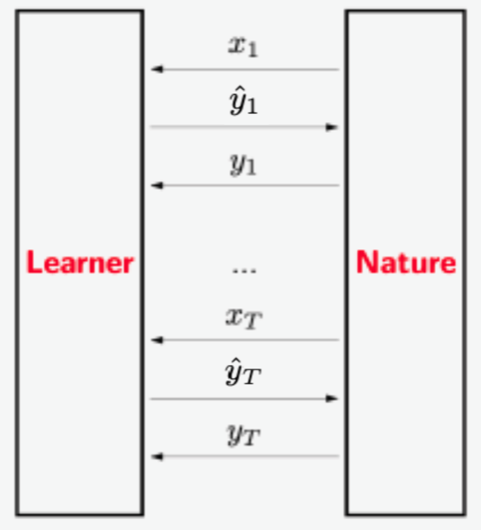
\includegraphics[width=2in]{figures/OLupdated.png}
    \caption{A representation of the online learning problem.}
    \label{lec15:fig:OLgame}
\end{figure}

Later, we will see that the manner in which nature generates  $(x_t, y_t)$ leads to different types of online learning. In the most adversarial setting of online learning, it is possible that the ``true label'' $y_t$ is not generated at the same time as $x_t$. The environment could generate the label $y_t$ depending on the prediction $\hat{y}_t$ made by the learner.  We can also see that Algorithm \ref{lec15:alg:gen-ol} is a very general framework as there are very few constraints on how $x_t$ and $y_t$ are generated.
    
\subsec{Evaluation of the learner}
Given this setup, a natural question to ask is how one can evaluate the performance of the learner. Intuitively, one could simply evaluate the learner's performance by computing the loss between the predicted label and the ``true'' label sent by the environment $\ell(y_t, \hat{y}_t)$. For the entire sequence of tasks, one can then evaluate in terms of the cumulative loss:
    \begin{align}
        \sum_{t=1}^T \ell(y_t, \yhat_t).
    \end{align}
    
However, as the environment can be adversarial, the task itself might be inherently hard and even the best possible learner fails to achieve a small loss. Hence, instead instead of using the cumulative loss for a learner by itself, we compare its performance against a suitable baseline, the ``best model in hindsight''. Assume that our learner comes from a set of hypotheses $\mathcal{H}$. Let us choose the hypothesis $h \in \mathcal{H}$ that minimizes the cumulative loss, i.e.
\begin{equation}
    h^\star = \argmin_{h \in \mathcal{H}} \sum_{t=1}^T \ell(y_t, h(x_t)).
\end{equation}

Note here that in minimizing the cumulative loss, the learner gets to see all the data points $(x_t, y_t)$ at once. The cumulative loss of $h^\star$ is the best we can ever hope to do, and so it would be better to compare the cumulative loss of the learner against it. (This approach is analogous to ``excess risk'', which tells how far the current model is away from the best we could hope for.) This measurement is denoted as \emph{regret}, and is formally defined as:
    \begin{align}
        \text{Regret} \overset{\Delta}{=} 
        \left[\sum_{t=1}^T \ell(y_t, \yhat_t)\right]
        - \underbrace{
        \left[\min_{h \in \mathcal{H}} \sum_{t=1}^T \ell(y_t, h(x_t))\right]
        }_{\text{best loss in hindsight}}
    \end{align}

Using this definition, if the best model in hindsight performs well, then the learner has more responsibility to learn to predict well in order to match up the performance of the baseline.
    
\subsec{The realizable case}
In general, if the environment is too powerful, leading the learner to a large loss, it will also hinder the best model in hindsight from doing well. On the other hand, there are settings where some members of the hypothesis class can actually do well. Such settings/problems are usually referred to as \textit{realizable}:

\begin{definition}[Realizable problem]
An online learning problem is \textit{realizable} (for a family of predictors $\mathcal{H}$) if there exists $h \in \mathcal{H}$ such that for any $T$, $\sum_{t = 1}^T \ell(y_t, h(x_t)) = 0$.
\end{definition}

Note that even though zero error is possible, this is still an interesting problem to consider because the $x_t$'s are not i.i.d. as they are in classical supervised learning. Hence, standard statistical learning theory does not apply, and there is still research to be done here.

\begin{example}
Consider a classification problem on $(x_t, y_t)$, and for simplicity assume $y_t \in \{0, 1\}$. Suppose there exists $h^\star \in \mathcal{H}$ such that we always have $y_t = \yhat^\star_t = h^\star(x_t)$. In this case, the problem is realizable. 
    
In this case, the learner can adopt a ``majority algorithm''. At each time, the learner maintains a set $V_t \subset \mathcal{H}$ so that $\sum_{t=1}^T \ell (y_t, h(x_t)) = 0$ for all $h \in V_t$, and $\hat{y}_t$ is simply the prediction made by the majority of $h \in V_t$. Based on the loss received, learners $h \in V_t$ that fail for time $t + 1$ will be eliminated from future $V_t$'s.
    
With this setup, we can see that for each wrong prediction made by the learner, at least half of the hypotheses $h \in V_t$ will be eliminated. Hence, $1 \leq |V_{t+1}| \leq |\mathcal{H}|2^{-M}$ where $M$ is the number of mistakes made so far. Thus, one has $M \leq \log |\mathcal{H}|$ by taking log on both sides of inequalities and rearrange.
    
Now, if one puts $\ell$ as the zero-one loss, the regret for this example will be
\begin{equation}
\text{Regret} = \sum_{t=1}^T \ell(y_t, h(x_t)) = M,
\end{equation}
so in this example, one has $\text{regret} \leq \log |\mathcal{H}|$, which is a non-trivial bound when $\mathcal{H}$ is finite.
\end{example}
    
As one can see in the example, the realizable case usually indicates that the problem is not too far out of reach. Indeed, for finite hypothesis classes and linear models, the realizable case is considered to be straightforward to solve. This is perhaps why most of the past literature has focused on non-realizable cases. However, the realizable case is still an interesting problem and perhaps a very good starting point when the model class is beyond linear models and when the loss function is no longer convex, because the $x_t$'s are not i.i.d. as they are in classical supervised learning. Hence, standard statistical learning theory does not apply, and there is still research to be done here.
 
In the rest of the chapter, we will only focus on the convex loss case, where we reduce online learning to online convex optimization. 
    
\sec{Online (convex) optimization (OCO)}

\textit{Online convex optimization (OCO)} is a particularly useful tool to get results for online learning. Many online learning problems (and many other types of problems!) can be reduced to OCO problems, which allow them to be solved and analyzed algorithmically. Algorithm \ref{lec15:alg:oco} describes the OCO problem, which is more general than the online learning problem. (Note: \textit{Online optimization (OO)} refers to Algorithm \ref{lec15:alg:oco} except that the $f_t$'s need not be convex. However, due to the difficulty in non-convex function optimization, most research has focused on OCO.)

    \begin{algorithm}\label{lec15:alg:oco}
    \caption{Online (convex) optimization problem}
    \For{$t = 1, ..., T$} {
        The learner picks some action $w_t \in \Omega$ from the action space $\Omega$\;
        The environment picks a (convex) function $f_t: \Omega \to [0, 1]$\;
        The learner suffers the loss $f_t(w_t)$ and observes the \emph{entire} loss function $f_t(\cdot)$.
        }
    \end{algorithm}
    
Essentially the learner is trying to minimize the function $f_t$ at each step. As with online learning, one evaluates the performance of learner in online optimization setting using the regret:
\begin{align}
\text{Regret} = \sum_{t=1}^T f_t(w_t) - 
\underbrace{\min_{w \in \Omega} \sum_{t=1}^T f_t(w)}_\text{best action in hindsight}.
\end{align}

At some level, OCO seems like an impossible task, since we are trying to minimize a function $f_t$ that we only get to see \textit{after} we have made our prediction! This is certainly the case for $t = 1$. However, as time goes on, we see more and more functions and, if future functions are somewhat related to past functions, we have more information to make better predictions. (And if the future functions are completely unrelated or contradictory to past functions, then the best action in hindsight would also be bad and therefore our algorithm does not have to do much.)

\subsec{Settings and variants of OCO}
There are multiple settings of the OCO network, which can vary the power of the environment and observations.

\begin{itemize}
    \item \underline{Stochastic setting:} $f_1,...,f_T$ are i.i.d samples from some distribution $P$. This corresponds to $(x_t, y_t)$ being i.i.d. in online learning. Under this setting, the environment is not adversarial.
    \item \underline{Oblivious setting:} $f_1,...,f_T$ are chosen arbitrarily but before the game starts. This corresponds to $(x_t, y_t$ being chosen before the game starts. In this setting, the environment can be adversarial but cannot be adaptive. The environment can choose these functions based on the learner's algorithm, but not the actual action if the learner's algorithm contains randomness. (This is the setting that we focus on in this course.)
    \item \underline{Non-oblivious/adaptive setting:} For all $t$, $f_t$ can depend on the learner's actions $w_1,...w_t$. Under this setting, the environment can be adversarial and adaptive. This is the most challenging setting because the environment is powerful enough to know not only the strategy of the learner, but also the exact choice the learner finally made. (Note however that If the learner is deterministic, the environment does not have more power here than in the oblivious setting. The oblivious adversary can simulate the game before the game starts, and chose the most adversarial input accordingly.)
\end{itemize}
 
\sec{Reducing online learning to online optimization}
There is a natural way to reduce the online learning problem to online optimization, with respect to a specific type of model $h_{w}$ parametrized by $w \in \Omega$. Recall that in online learning problem, the learner predicts $y_t$ upon receiving $x_t$. If the learner possesses oracle to solve online optimization problem, the learner can consult the oracle to obtain $w_t$, the parameter of the model as in online optimization problem, and then predict $\hat{y}_t = h_{w_t}(x_t)$.

In the next two subsections, we give two examples of how an online learning problem can be reduced to an OCO problem.
    
\subsec{Example: Online learning regression problem}

Consider the regression model $h_w(x) = w^\top x$ parameterized by $w$ in parameter space $\Omega$ with squared error loss $\ell$. Here is the online learning formulation of the regression problem:

\begin{algorithm}
\caption{Online learning regression problem}
\For{$t = 1, ..., T$} {
The learner receives $x_t \in \R^d$ from the environment\;
The learner predicts $\yhat_t$\;
The environment selects $y_t$ and sends it to the learner\;
The learner suffers loss $\ell(y_t, \yhat_t) = (y_t-\yhat_t)^2$.
}
\end{algorithm}

This can be reduced to the OCO problem in the following way:

\begin{algorithm}
\caption{OCO formulation of regression problem}
\For{$t = 1, ..., T$} {
The learner receives $x_t \in \R^d$ from the environment\;
The learner gives $x_t$ to the OCO solver and obtains $w_t \in \R^d$\;
The learner predicts $\hat{y}_t = h_{w_t}(x_t) = w_t^\top x_t$\;
The environment selects $y_t$ and sends it to the learner\;
The learner suffers loss $(y_t - h_{w_t}(x_t))^2$\;
With $(x_t, y_t)$ observed, the learner can reconstruct the loss function $f_t(w) = (y_t -h_{w}(x_t))^2$ and give it to the OCO solver.
}
\end{algorithm}

In this example, we have the following correspondence:
\begin{itemize}
\item $f_t$ in online optimization $\leftrightarrow$ squared error loss functions for $(x_t, y_t)$.
\item $w_t$ in online optimization $\leftrightarrow$ parameters of the linear model $h_{w_t}$.
\end{itemize}
    
Since $h_w(\cdot)$ is linear, the corresponding squared error loss function $f_t$ are convex, and so we have effectively reduced the online linear regression problem to an online \emph{convex} optimization problem.
    
Notice that in the previous example, the loss function $f_t$ actually depends on the label $y_t$, which demonstrates that the key challenge in online optimization is that the function $f_t$ is unknown to the learner when the prediction $\hat{y}_t$ is made.
    
\subsec{Example: The expert problem}
Suppose we wish to predict tomorrow's weather and 10 different TV channels provide different forecasts. Which one should we follow? Formally, consider a finite hypothesis class $\mathcal{H}$, where each $h \in \mathcal{H}$ represents an expert, and we wish to choose a $h_t$ wisely at each time step. For simplicity, we assume the prediction is binary, i.e. $\hat{y} \in \{0, 1\}$, and suppose the loss function is 0-1 loss. (The problem can easily be generalized to more general predictions and losses.) The problem is outlined in Algorithm \ref{lec15:alg:expert_discrete}.

\begin{algorithm}[h]
\caption{The expert problem}
\label{lec15:alg:expert_discrete}
\For{$t = 1, ..., T$}{
The learner obtains predictions from $N$ experts\;
The learner chooses to follow prediction of one of the experts $i_t \in [N]$\;
The environment gives the learner the true value. The learner is thus able to learn the loss of each of the experts: $\ell_t \in \{0, 1\}^N$\;
The learner suffers the loss of the expert which was chosen: $\ell_t(i_t)$.
}
\end{algorithm}

We want to design a method that chooses $i_t$ for each step (line 3 in Algorithm \ref{lec15:alg:expert_discrete}) to minimize the regret:
\begin{equation}
\text{Regret} \overset{\Delta}{=} \mathbb{E}\left[
\sum_{t=1}^T \ell_t(i_t)
- \underbrace{\min_{i \in [N]} \sum_{t=1}^T \ell_t(i)}_\text{the best expert in hindsight}
\right],
\end{equation}
where the expected value is over $i_t$, thus covering the case where the $i_t$'s could be random.
    
To make the expert problem amenable to reduction to OCO, we introduce idea of a \textit{continuous action space}. Instead of choosing $i_t$ from $\Omega = [N]$, the learner chooses a distribution $p_t$ from the $N$-dimensional simplex $\Delta(N) = \left\{p \in \R^N : \norm{p}_1 = 1, p \geq 0 \right\}$. The learner then samples $i_t \sim p_t$. With this formulation, instead of selecting particular expert $i_t$ to follow, the learner adjusts the belief $p_t$, and samples from the distribution to choose which expert to follow. Algorithm \ref{lec15:alg:expert_randomized} outlines this procedure. Note that the loss is the expected loss $\mathbb{E}_{i \sim p_t}[\ell_t(i)]$ instead of the sampled $\ell_t(i_t)$.

\begin{algorithm}
\caption{The expert problem with continuous action}
\label{lec15:alg:expert_randomized}
\For{$t = 1, ..., T$}{
The learner obtains predictions from $N$ experts\;
The learner chooses a distribution $p_t \in \Delta(N)$\;
The learner samples one expert $i_t \sim p_t$\;
The environment gives the learner the true value and the loss/error of all experts: $\ell_t \in \{0, 1\}^N$\;
The learner suffers expected loss $\sum_{i\in[N]} p_t(i) \ell_t(i) = \langle p_t, \ell_t \rangle$\;
}
\end{algorithm}
    
With the continuous action space, it is easy to reduce the expert problem to an OCO: see Algorithm \ref{lec15:alg:expert_discrete_oco}. (The problem is convex since the loss function is convex and the parameter space $\Delta(N)$ is convex.)

\begin{algorithm}[h]
\caption{The expert problem}
\label{lec15:alg:expert_discrete_oco}
\For{$t = 1, ..., T$}{
The learner obtains predictions from $N$ experts\;
The learner invokes the OCO oracle to obtain $p_t \in \Delta(N)$\;
The learner chooses to follow prediction of one of the experts $i_t \in [N]$\;
The environment gives the learner the true value. The learner is thus able to learn the loss of each of the experts: $\ell_t \in \{0, 1\}^N$\;
The learner suffers the loss of the expert which was chosen: $\ell_t(i_t)$.
The learner can reconstruct the loss function $f_t (p) = \langle p, \ell_t \rangle$ and give it to the OCO oracle.
}
\end{algorithm}

In this setting, one can rewrite the regret as:
\begin{align}
\text{Regret} &= \sum_{t=1}^T \langle p_t, \ell_t \rangle - \min_{i\in[N]}\sum_{t=1}^T \ell_t(i)  \\
&= \sum_{t=1}^T \langle p_t, \ell_t \rangle - \min_{p \in \Delta(N)}\sum_{t=1}^T \langle p, \ell_t \rangle \label{lec15:eqn:changearg} \\
&= \sum_{t=1}^T f_t(p_t) - \min_{p \in \Delta(N)}\sum_{t=1}^T f_t(p). \label{lec15:eqn:regret}
\end{align}

We obtain \eqref{lec15:eqn:changearg} because
\begin{align}
\sum_{t=1}^T \langle p, \ell_t \rangle &=  \left\langle p,  \sum_{t=1}^T\ell_t \right\rangle \geq \min_{i \in [N]} \left[ \sum_{t=1}^T \ell_t (i) \right],
\end{align}
with equality for the probability distribution $p(i) =1$ when $i = \text{argmin}_i \left[ \sum_{t=1}^T \ell_t (i) \right]$ and $p(i) = 0$ otherwise, and \eqref{lec15:eqn:regret} is by definition of $f_t$.


\sec{Reducing online learning to batch learning}    
In this section, we present a reduction from online learning to standard supervised learning problem, also known as the ``batch problem'' in this literature.

As in the standard supervised learning setting, consider an i.i.d dataset $\{(x_t, y_t)\}_{t=1}^T$ and some parameter $w$. Let $L(w)$ and $\hatL(w)$ be the population loss and empirical loss respectively. For simplicity, assume $|\ell((x_i, y_i), w)| \leq 1$. The theorem below establishes a link between the regret obtained in online learning and the excess risk obtained in the batch setting.
    
\begin{theorem}[Relationship between excess risk and regret]
Assume $\ell((x, y), w)$ is convex. Suppose we run an online learning algorithm on the dataset $\{(x_i, y_i)\}_{i=1}^T$ and obtain a sequence of models $w_1, \dots, w_T$, and regret $R_T$. Let $\overline{w} = \frac{1}{T} \sum_{i=1}^T w_i$, then the excess risk of $\overline{w}$ can be bounded above:
\begin{align}
L(\overline{w}) - L(w^\star) \leq \frac{R_T}{T} + \tilO\left(\frac{1}{\sqrt{T}}\right), \label{lec15:eqn:lec15_ol_gen_bound}
\end{align}
where $w^\star = \argmin_{w \in \Omega} L(w)$.
\end{theorem}

Here are some intuitive interpretations of the theorem:

    \begin{itemize}
        \item If $R_T = O(T)$, then we have some non-trivial result. Otherwise, the bound in \eqref{lec15:eqn:lec15_ol_gen_bound} is increasing $T$ and does not provide any useful information.
        \item If the batch problem has a $1 / \sqrt{T}$ generalization bound, then the best you can hope for in online learning is $R_T = O(\sqrt{T})$.
        \item If the batch problem has a $1 / T$ generalization bound, you can hope for $O(1)$ regret (or $\tilO(1)$ regret in some cases).
        \item We often have $O(\sqrt{T})$ excess risk supervised learning problems; hence it is reasonable to expect $O(\sqrt{T})$ regret in online learning problems.
    \end{itemize}
    
\sec{Follow-the-Leader (FTL) algorithm} \label{lec15:sec:FTL}
In this section, we analyze an algorithm called ``Follow-the-Leader'' (FTL) for OCO, which is intuitive but fails to perform well in many cases.

The FTL algorithm behaves as its name suggests: it always selects the action $w_t$ such that it minimizes the historical loss the learner has seen so far, i.e.
\begin{equation}
w_t = \argmin_{w \in \Omega} \sum_{i=1}^{t-1} f_i(w).
\end{equation}

We now demonstrate how the FTL algorithm can fail for the expert problem. In the expert problem, $f_t(p) = \langle p, \ell_t \rangle$, so 
    \begin{align}
        p_t &= \argmin_{p \in \Delta(N)} \sum_{i=1}^{t-1} f_i(p) \\
        &= \argmin_{p \in \Delta(N)} \sum_{i=1}^{t-1} \langle\ell_i, p\rangle \\
        &= \argmin_{p \in \Delta(N)} \left\langle\sum_{i=1}^{t-1}\ell_i, p\right\rangle.
    \end{align}

The minimizer $p \in \Delta(N)$ is a point-mass probability, with the point mass at the smallest coordinate of $\sum_{i=1}^{t-1} \ell_i$. This gives regret
\begin{equation}
\text{Regret} = \sum_{i=1}^{t-1} \ell_i(i_t),
\quad \text{ where } i_t = \argmin_{j \in [N]} \sum_{i=1}^{t-1}\ell_i(j).
\end{equation}
    
Now, consider the following example: suppose we have only two experts. Suppose expert 1 makes perfect predictions on even days while expert 2 makes perfect predictions on odd days. Assume also that the FTL algorithm chooses expert 1 to break ties (this is not an important point but makes the exposition simpler.) In this setting, the FTL algorithm always selects the \textit{wrong} expert to follow. A few rounds of simulation of this example is shown in Table \ref{lec15:tab:counter example}.

    \begin{table}[h]
        \caption{An example where FTL fails}
        \label{lec15:tab:counter example}
        \medbreak
        \centering
        \small
        \begin{tabular}{l|c c c c c c}
        \toprule
        Day & 1 & 2 & 3 & 4 & $\dots$ & $\dots$ \\
        \midrule 
        Expert 1's loss & 1 & 0 & 1 & 0 & $\dots$ & $\dots$ \\
        Expert 2's loss & 0 & 1 & 0 & 1 & $\dots$ & $\dots$ \\
        \midrule 
        \midrule 
        FTL choice $i_t$ & 1 & 2 & 1 & 2 & 1 & $\dots$ \\
        \bottomrule
        \end{tabular}
    \end{table}

The best expert in hindsight has a loss of $T/2$ (choosing either expert all the time incurs this loss, and so the regret of the FTL algorithm is $T - T/2 = T/2 = \Theta(T)$. The main reason for FTL's failure is that is a deterministic algorithm driven by an extreme update, with no consideration on potential domain shift (it always selects the best expert based on the past with no consideration of the potential next $f_t$). Knowing its deterministic strategy, the environment can easily play in an adversarial manner. To perform better in a problem like this, we need some randomness to hedge risk.
	% reset section counter
%\setcounter{section}{0}

%\metadata{lecture ID}{Your names}{date}
\metadata{16}{Kevin Guo}{Mar 10th, 2021}

% ===============================================
\sec{Be-the-leader (BTL) algorithm}

A better strategy is called \textit{``Be the Leader'' (BTL)}.  At time $t$, the BTL strategy chooses the action that would have performed best on $f_1, \cdots, f_{t-1}$ \textit{and} $f_t$.  In other words, the BTL action at time $t$ is $w_{t+1}$, as defined for the FTL algorithm. Note that this is an ``illegal'' choice for the action because $w_{t+1}$ depends on $f_t$: in online convex optimization, the action at time $t$ is required to be chosen \textit{before} seeing the function $f_t$.  Nevertheless, we can still gain some useful insights by analyzing this procedure. In particular, the following lemma shows that the BTL strategy is worth emulating because it achieves very good regret.

\begin{lemma}\label{lec16:lem:btl_regret}
The BTL strategy has non-positive regret. That, is, if $w_t$ is defined as in the FTL algorithm, then
\begin{align}
\text{BTL regret} = \sum_{t = 1}^T f_t(w_{t + 1}) - \min_{w \in \Omega} \sum_{t = 1}^T f_t(w) \leq 0, \label{lec16:eqn:btl_regret}
\end{align}
for any $T$ and any sequence of functions $f_1, \cdots, f_T$.
\end{lemma}

\begin{proof}
We prove the lemma by induction on $T$. \eqref{lec16:eqn:btl_regret} holds trivially for $T = 1$. Suppose that \eqref{lec16:eqn:btl_regret} holds for all $t \leq T - 1$ and any $f_1, \cdots, f_{T-1}$.  Now we wish to extend \eqref{lec16:eqn:btl_regret} to time $t = T$.  Let $f_T$ be any function.  Since $w_{T+1} = \argmin_w \sum_{t = 1}^T f_t(w)$, we can write:
\begin{align}
\sum_{t = 1}^{T} f_t(w_{t+1}) - \min_{w \in \Omega} \sum_{t = 1}^{T} f_t(w) &= \sum_{t = 1}^T f_t(w_{t+1}) - \sum_{t = 1}^T f_t(w_{T+1})\\
&= \sum_{t = 1}^{T - 1} f_t(w_{t+1}) - \sum_{t = 1}^{T - 1} f_t(w_{T+1}) &\text{(final summands cancel)}\\
&\leq \sum_{t = 1}^{T - 1} f_t(w_{t+1}) - \min_{w \in \Omega} \sum_{t = 1}^{T - 1} f_t(w)\\
&\leq 0. &\text{(induction hypothesis)}
\end{align}
\end{proof}

A useful consequence of this lemma is a regret bound for the FTL strategy.

\begin{lemma}
\label{lec16:lem:ftl_regret}
\textup{(FTL regret bound)} Again, let $w_t$ be as in the FTL algorithm. The FTL strategy has the regret guarantee
\begin{align}
\text{FTL regret} = \sum_{t = 1}^T f_t(w_t) - \min_{w \in \Omega} \sum_{t = 1}^T f_t(w) \leq \sum_{t = 1}^T [f_t(w_t) - f_t(w_{t+1})].
\end{align}
\end{lemma}

\begin{proof}
\begin{align}
\text{FTL regret} &= \sum_{t = 1}^T f_t(w_t) - \min_{w \in \Omega} \sum_{t = 1}^T f_t(w) \\
&= \sum_{t = 1}^T f_t(w_{t+1}) - \min_{w \in \Omega} \sum_{t = 1}^T f_t(w) + \sum_{t = 1}^T [f_t(w_t) - f_t(w_{t+1})] \\
&\leq 0 + \sum_{t = 1}^T [f_t(w_t) - f_t(w_{t+1})],
\end{align}
where the last inequality is due to \eqref{lec16:eqn:btl_regret}.

\end{proof}

Lemma \ref{lec16:lem:ftl_regret} tells us that if terms $f_t(w_t) - f_t(w_{t+1})$ are small (e.g. $w_t$ does not change much from round to round), then the FTL strategy can have small regret. It suggests that the player should adopt a \textit{stable} policy, i.e. one where the terms $f_t(w_t) - f_t(w_{t+1})$ are small.  It turns out that following this intuition will lead to a strategy that improves the regret all the way to $O(\sqrt{T})$ in certain cases.

% ===============================================
\sec{Follow-the-regularized-leader (FTRL) strategy}

Now, we discuss a OCO strategy aims to improve the stability of FTL by controlling the differences $f_t(w_t) - f_t(w_{t+1})$. To describe the method, we will first need a preliminary definition.

\begin{definition}
We say that a differentiable function $\phi : \Omega \mapsto \R$ is \textit{$\alpha$-strongly-convex} with respect to the norm $|| \cdot ||$ on $\Omega$ if we have 
\begin{equation}\label{lec16:eqn:strongly-convex}
\phi(x) \geq \phi(y) + \langle \nabla f(y), x - y \rangle + \frac{\alpha}{2} \norm{x - y}^2
\end{equation}
for any $x, y \in \Omega$.
\end{definition}

\begin{remark}
If $\phi$ is convex, then we know that $f(x)$ has a linear lower bound $\phi(y) + \langle \nabla f(y), x - y \rangle$. Being $\alpha$-strong-convex means that $f(x)$ has a quadratic lower bound, the RHS of \eqref{lec16:eqn:strongly-convex}. This quadratic lower bound is very useful in proving theorems in optimization.
\end{remark}

\begin{remark}
If $\nabla^2 f(y) \succeq \alpha I$ for all $y$, then $f$ is $\alpha$-strongly-convex. This follows directly from writing the second-order Taylor expansion of $f$ around $y$.
\end{remark}

Given a $1$-strongly-convex function $\phi(\cdot)$, which we call a \textit{regularizer}, we can implement the \textit{``Follow the Regularized Leader'' (FTRL)} strategy.  At time $t$, this strategy chooses the action
\begin{align}
w_t = \argmin_{w \in \Omega} \left[ \sum_{i = 1}^{t -1} f_i(w) + \frac{1}{\eta} \phi(w) \right], \label{lec16:eqn:ftrl}
\end{align}
where $\eta > 0$ is a tuning parameter that we will tune later.

\subsec{Regularization and stability}

To understand why we might use the FTRL policy, we first establish that it achieves the intended goal of controlling the differences $f_t(w_t) - f_t(w_{t+1})$. Actually, we will show a more general result that adding a regularizer induces stability for any convex objective.

\begin{lemma}
\label{lec16:lem:regularizers_stability}
\textup{(Regularizers induce stability)} Let $F$ and $f$ be functions taking $\Omega$ into $\R$, and assume that $F$ is $\alpha$-strongly-convex with respect to the norm $\norm{\cdot}$ and that $f$ is convex.  Let $w = \argmin_{z \in \Omega} F(z)$ and $w' = \argmin_{z \in \Omega} [f(z) + F(z)]$.  Then
\begin{equation}\label{lec16:eqn:regularizers_stability}
0 \leq f(w) - f(w') \leq \frac{1}{\alpha} \norm{\nabla f(w)}_*^2,
\end{equation}
where $\norm{\cdot}_*$ is the dual norm of $\norm{\cdot}$.
\end{lemma}

\begin{proof}
By strong convexity,
\begin{align}
F(w') - F(w) &\geq \langle \nabla F(w), w' - w \rangle + \frac{\alpha}{2} \norm{w - w'}^2 \\
&\geq \frac{\alpha}{2} \norm{w - w'}^2,
\end{align}
where in the second step we used the fact that the KKT optimality conditions for $w$ imply $\langle \nabla F(w), w' - w \rangle \geq 0$. (Informally, if $\Omega = \R^d$, then $\nabla F(w) = 0$ as $w$ minimizes $F$. If $\Omega$ is a convex subset of $\R^d$, then the gradient $\nabla F(w)$ must be perpendicular to the tangent to $\Omega$ at $w$; otherwise, we could move in the direction of the negative gradient and project back to the set $\Omega$ to lower the value of $F$.) Since $F + f$ is also $\alpha$-strongly convex, exactly the same argument implies:
\begin{align}
[F(w) + f(w)] - [F(w') + f(w')] \geq \frac{\alpha}{2} \norm{w - w'}^2.
\end{align}
Adding these two inequalities gives
\begin{align}
f(w) - f(w') \geq \alpha \norm{w - w'}^2. \label{lec16:eqn:lower_bound}
\end{align}
Since this lower bound is clearly positive, this shows $0 \leq f(w) - f(w')$.

Next, we prove the upper bound on $f(w) - f(w')$. Rearranging the inequality \eqref{lec16:eqn:lower_bound}, we obtain
\begin{align}
\norm{w - w'} \leq \sqrt{\frac{1}{\alpha} [f(w) - f(w')]}. \label{lec16:eqn:upper_bound}
\end{align}
Since $f$ is convex, we have $f(w') \geq f(w) + \langle \nabla f(w), w' - w \rangle$.  Rearranging this gives
\begin{align*}
f(w) - f(w') &\leq \langle \nabla f(w), w - w' \rangle\\
&\leq \norm{\nabla f(w)}_* \cdot \norm{w - w'} &\text{(by Cauchy-Schwarz)} \\
&\leq \norm{\nabla f(w)}_* \sqrt{ \frac{1}{\alpha} [f(w) - f(w')]}. &\text{(by \eqref{lec16:eqn:upper_bound})}
\end{align*}
Since $f(w) - f(w') \geq 0$, we can square both sides of this inequality to conclude that
\begin{equation}
[f(w) - f(w')]^2 \leq || \nabla f(w) ||_*^2 \frac{1}{\alpha} [f(w) - f(w')].
\end{equation}
Dividing both sides of this expression by $f(w) - f(w')$ gives the desired upper bound.
\end{proof}

\begin{remark}
Consider the special case where $\nabla f(w) = 0$. In this situation, $w$ is the minimizer of both $F$ and $f$, and hence is the minimizer of $F + f$. This implies that $w = w'$, and the inequalities in \eqref{lec16:eqn:regularizers_stability} become equalities.
\end{remark}

\subsec{Regret of FTRL}
We are now ready to prove a regret bound for the FTRL procedure, based on the idea that strongly convex regularizers induce stability.

\begin{theorem}\label{lec16:thm:ftrl_regret}
\textup{(Regret of FTRL)} Let $\phi$ be a 1-strongly-convex regularizer with respect to the norm $\norm{\cdot}$ on $\Omega$.  Then the FTRL algorithm (\ref{lec16:eqn:ftrl}) satisfies the regret guarantee
\begin{align}
\text{FTRL regret} = \sum_{t = 1}^T f_t(w_t) - \argmin_{w \in \Omega} \sum_{t = 1}^T f_t(w)  \leq \frac{D}{\eta} + \eta \sum_{t = 1}^T \norm{\nabla f_t(w_t)}_*^2,
\end{align}
where $D = \max_{w \in \Omega} \phi(w) - \min_{w \in \Omega} \phi(w)$.
\end{theorem}

\begin{remark}
Suppose that for all $t$ and $w$, we have the uniform bound $|| \nabla f_t(w) ||_* \leq G$.  Then Theorem \ref{lec16:thm:ftrl_regret} implies that the regret is upper bounded by $D / \eta + \eta G T$.  Optimizing this upper bound over $\eta$ by taking $\eta = \sqrt{\dfrac{D}{TG^2}}$ gives the guarantee
\begin{equation}\label{lec17:eqn:ftrl-regret-ub}
\text{FTRL regret} \leq 2 \sqrt{D G} \times \sqrt{T}.
\end{equation}
In other words, optimally-tuned FTRL can achieve $O(\sqrt{T})$ regret in many cases.
\end{remark}

\begin{proof}
For convenience, define $f_0(w) = \phi(w) / \eta$.  Then the FTRL policy can be written as
\begin{equation}
w_t = \argmin_{w \in \Omega} \sum_{i = 0}^{t - 1} f_i(w),
\end{equation}
i.e. FTRL is just FTL with an additional ``round'' of play at time zero. Thus, by Lemma \ref{lec16:lem:ftl_regret} with time starting from $t = 0$, we have
\begin{align}
\sum_{t = 0}^T f_t(w_t) - \argmin_{w \in \Omega} \sum_{t = 0}^T f_t(w) &\leq \sum_{t = 0}^T [f_t(w_t) - f_t(w_{t+1})].
\end{align}
For any $t \geq 1$, applying Lemma \ref{lec16:lem:regularizers_stability} with $F(w) = \sum_{i = 0}^{t-1} f_i(w)$ (which is $1/\eta$-strongly-convex) and $f(w) = f_t(w)$ gives the bound $f_t(w_t) - f_t(w_{t+1}) \leq \eta || \nabla f_t(w_t) ||_*^2$.  Plugging this into the preceding display gives the upper bound:
\begin{align}
\sum_{t = 0}^T f_t(w_t) - \argmin_{w \in \Omega} \sum_{t = 0}^T f_t(w) &\leq f_0(w_0) - f_0(w_1) + \eta \sum_{t = 1}^T \norm{\nabla f_t(w_t)}_*^2. \label{lec16:eqn:ftrl_ub}
\end{align}

Next, we need to relate the LHS of the above display (which starts at time $t = 0$) to the actual regret of FTRL (which starts at time $t = 1$). To do this, define $w^* = \argmin_{w \in \Omega} \sum_{t = 1}^T f_t(w)$. Then,
\begin{align}
\sum_{t = 0}^T f_t(w_t) - \argmin_{w \in \Omega} \sum_{t = 0}^T f_t(w) &\geq \sum_{t = 0}^T f_t(w_t) - \sum_{t = 0}^T f_t(w^*)\\
&= f_0(w_0) - f_0(w^*) + \underbrace{\left( \sum_{t = 1}^T f_t(w_t) - \argmin_{w \in \Omega} \sum_{t = 1}^T f_t(w)  \right)}_{\text{Regret of FTRL}}.
\end{align}
Combining this inequality with (\ref{lec16:eqn:ftrl_ub}) gives
\begin{align}
\text{Regret of FTRL} &\leq f_0(w_0) - f_0(w_1) + f_0(w^*) - f_0(w_0) + \eta \sum_{t = 1}^T \norm{\nabla f_t(w_t)}_*^2\\
&= \frac{\phi(w^*) - \phi(w_1)}{\eta} + \eta \sum_{t = 1}^T \norm{\nabla f_t(w_t)}_*^2\\
&\leq \frac{D}{\eta} + \eta \sum_{t = 1}^T \norm{\nabla f_t(w_t)}_*^2.
\end{align}
This concludes the proof of the theorem.
\end{proof}

\subsec{Applying FTRL to online linear regression}

We apply the FTRL algorithm to a concrete machine learning problem. Let $\Omega = \{ \omega \, : \, \norm{w}_2 \leq 1 \}$, and let $f_t(\omega) = \tfrac{1}{2}(y_t - \omega^{\top} x_t)^2$ for some observation pair $(x_t, y_t)$ satisfying $\norm{x_t}_2 \leq 1$ and $|y_t| \leq 1$.  This corresponds to a problem where we are trying to make accurate predictions using a linear model, but we do not assume any structure on the observation sequence $(x_t, y_t)$ beyond boundedness.

Consider using FTRL in this problem with a ridge regularizer, $\phi(\omega) = \tfrac{1}{2} \norm{w}_2^2$.  One can check that $\phi$ is 1-strongly-convex with respect to the $\ell_2$-norm, and also that $D = \max_{\omega \in \Omega} \phi(\omega) - \min_{\omega \in \Omega} \phi(\omega) = \tfrac{1}{2}$.  Moreover, for all $t$ and $w$ we have 
\begin{align}
\nabla f_t(w) &= - (y_t - w^\top x_t) x_t, \\
\norm{\nabla f_t(w)}_2 &\leq |y_t - w^\top x_t| \cdot \norm{x_t}_2 \\
&\leq 2 \cdot 1 = 2.
\end{align}
Therefore, by choosing $\eta = \sqrt{1/(8T)}$ and applying the FTRL regret theorem (Theorem \ref{lec16:thm:ftrl_regret}), we can obtain the regret guarantee
\begin{align}
\sum_{t = 1}^T (y_t - w_t^{\top} x_t)^2 - \min_{|| w ||_2 \leq 1} \sum_{t = 1}^T  (y_t - w^{\top} x_t)^2 \leq 4 \sqrt{T}.
\end{align}

\subsec{Applying FTRL to the expert problem}

For the expert problem, recall that the action space is $\Delta (N)$ and $f_t = \langle \ell_t , p \rangle$, where $\ell_t \in [0,1]^N$. As a first attempt at applying FTRL to this problem, we set $\phi (p) = \frac{1}{2}\norm{p}_2^2$. With this choice,
\begin{align}
D &= \max_{p \in \Delta(N)} \phi (p) - \min_{p \in \Delta(N)} \phi (p) \\
&\leq \max_{p \in \Delta(N)} \frac{1}{2}\norm{p}_2^2 \\
&\leq \max_{p \in \Delta(N)} \frac{1}{2}\norm{p}_1^2 \\
&= \frac{1}{2}.
\end{align}

Also,
\begin{align}
\norm{\nabla f_t}_2 &= \norm{\ell_t}_2 \leq \sqrt{N}.
\end{align}

Thus, the regret bound is $O(G\sqrt{DT}) = O(\sqrt{NT})$. This is optimal dependency on $T$, but not good dependency on $N$.

Next, we show that if we change our regularization, we can get a better regret guarantee which is logarithmic in $N$, i.e., the regret is $O(\sqrt{(log N) \cdot T})$. The new regularizer we choose is the \textit{(negative) entropy regularizer}:
\begin{equation}
\phi(p) = -H(p) = \sum_{j=1}^N p(j)\log p(j),
\end{equation}
where $p \in \Delta(N)$ is in the set of distributions over $[N]$. We first introduce the following nice property of this regularizer:
\begin{lemma}
	$\phi(p)$ defined above is 1-strongly convex with respective to the $\ell_1$ norm $\|\cdot\|_1$. 
\end{lemma}

\begin{proof}
By definition of strong convexity, we need to show that for all $p, q \in \Delta(N)$,
\begin{equation}\label{lec17:eqn:entropy-sc}
\phi(p) - \phi(q) - \langle \nabla \phi(q), p-q\rangle \geq \frac{1}{2} \|p-q\|_1^2.
\end{equation}
	
From direct computation, we know the gradient of $\phi(q)$ is 
\begin{equation}
\nabla\phi(q) = \begin{bmatrix} 1+\log q(1)\\\cdots \\ 1+\log q(N) \end{bmatrix}.
\end{equation}
	
Plugging this into the LHS of \eqref{lec17:eqn:entropy-sc}, we get
\begin{align}
&\phi(p) - \phi(q) - \langle \nabla \phi(q), p-q\rangle  \\
=& \sum_{j=1}^N p(j)\log p(j) - \sum_{j=1}^N q(j)\log q(j) - \sum_{j=1}^N \left(1 + \log q(j)\right)\left(p(j) - q(j)\right) \\
=& \sum_{j=1}^N p(j)\log p(j) - \sum_{j=1}^N p(j)\log q(j) - \sum_{j=1}^N \left(p(j) - q(j)\right)\\
=& \sum_{j=1}^N p(j) \log \frac{p(j)}{q(j)} \label{lec17:eqn:entropy-sc-proof} \\
=& KL(p||q),
\end{align}
where $KL(p || q)$ is the KL-divergence between $p$ and $q$. (We used the fact that $\sum_{j=1}^N p(j) = \sum_{j=1}^N q(j) = 1$ to get \eqref{lec17:eqn:entropy-sc-proof}.) Finally, we finish the proof by applying Pinsker's inequality: $KL(p||q) \geq \frac{1}{2} \norm{p-q}_1^2$. 
	
\end{proof}

Hence, $\phi$ is a satisfies the condition on the regularizer for our FTRL regret guarantee. To obtain the regret bound \eqref{lec17:eqn:ftrl-regret-ub}, we also need to bound $D = \sup \phi(p) - \inf \phi(p)$ and $G = \sup \|\nabla f_t(w)\|_\infty$ (since $\|\cdot\|_\infty$ is the dual norm of $\|\cdot \|_1$ ). Since negative entropy is always non-positive and (positive) entropy is always bounded above by $\log N$, we bound $D$ with
\begin{equation} 
D = \sup \phi(p) - \inf \phi(p) \leq -\inf \phi (p) = -\inf (-H(p)) = \sup (H(p)) \leq \log N,
\end{equation}
and we bound $G$ with
\begin{equation}
G = \|\nabla f_t(w)\|_\infty = \|l_t\|_\infty \leq 1.
\end{equation}

Plugging these two into the regret bound \eqref{lec17:eqn:ftrl-regret-ub} we get bound $O(\sqrt{(\log N) \cdot T})$. 

Thus far, we have looked at FTRL and the expert problem abstractly: at each time $t$ we choose action $p_t$ based on the update
\begin{equation}
p_t = \argmin_{p \in \Delta(N)} \sum_{i=1}^{t+1} f_t(p) - \frac{1}{\eta} H(p).
\end{equation}

\textbf{Can we get an exact analytical solution for $p_t$?} Since we are minimizing a convex function, we can call some off-the-shelf convex optimization algorithm to solve this at each step. Another way is to write down the KKT conditions and solve that set of equations.  Instead, we will show that there exists much simpler ways to solve this update. In particular, we will be using the \textit{Gibbs variational principle}, which is essentially the KKT conditions under the hood.

\begin{lemma}[Gibbs variational principle] \label{lec17:lem:gibbs}
Let $\nu, \mu$ be probability distributions on $[N]$. Then 
\al{\sup_\nu \left(\Exp_\nu[f] - KL(\nu||\mu)\right) = \log \Exp_\mu \left[e^f\right],} where $\Exp_\nu[f] = \Exp_{x \sim \nu} [f(x)] = \langle v, f\rangle$ and $\Exp_\mu \left[e^f\right] = \Exp_{x \sim \mu}  \left[e^{f(x)}\right]$. Moreover, the optimal solution is attained at \al{\nu(x) \propto \mu(x) \cdot e^{f(x)}.}
\end{lemma}

Intuitively, Lemma~\ref{lec17:lem:gibbs} says that taking the supremum over distributions $\mu$ of a linear function plus the KL divergence as the regularizer will give us the same distribution as exponentiating $f$. 

If we take $\mu$ to be the uniform distribution on $[N]$ and replace $f$ with $-f$ in Lemma~\ref{lec17:lem:gibbs}, we get the following corollary:

\begin{corollary}\label{lec17:cor:gibbs}
	Let $\nu$ be a probability distribution. Then, 
	$\Exp_\nu[f] - H(\nu)$ is minimized at $\nu(x) \propto e^{-f(x)}$.
\end{corollary} 

\begin{proof}
When $\mu$ is uniform distribution, we have
\begin{align}
KL(\nu||\mu) &= \sum_x \nu(x) \log \frac{\nu(x)}{\mu(x)} \\
&= \log N - \sum_x \nu(x) \log \frac{1}{\nu(x)} \\
&= \log N - H(\nu).
\end{align}

So $\sup_\nu \left(\Exp_\nu[-f] - KL(\nu||\mu)\right) = -\inf_\nu \left(\Exp_\nu[f] - H(\nu) + \log N\right)$. This means that the value of $\nu$ that attains the infimum of $\Exp_\nu[f] - H(\nu)$ is the same $\nu$ attaining the supremum of $\Exp_\nu[-f] - KL(\nu||\mu)$, which by Lemma~\ref{lec17:lem:gibbs} is proportional to $e^{-f(x)}$.
\end{proof}

We now apply the Gibbs variational principle to the expert problem. Notice that our FTRL update for the expert problem at time $t$ can be written as
\begin{equation}
\argmin_{p_t \in \Delta(N)} \l\langle \sum_{i=1}^{t-1}l_i, p_t \r\rangle - \frac{1}{\eta}H(p_t) = \argmin_{p_t \in \Delta(N)} \l\langle\eta \sum_{i=1}^{t-1}l_i, p_t \r\rangle - H(p_t),
\end{equation}
where $l_i$ is the vector of expert losses at time $i$. Letting $f = \eta \sum_{i=1}^{t-1} l_i$, we know from Corollary~\ref{lec17:cor:gibbs} that the minimizer is attained at $p_t \propto \exp \l(-\eta \sum_{i=1}^{t-1}l_i \r)$, or equivalently,  
\begin{equation}
p_t(j) = \frac{\exp(-\eta L_t(j))}{\sum_{k=1}^N \exp(-\eta L_t(k))},
\end{equation}
where $L_t = \sum_{i=1}^{t-1}l_i$ is the cumulative loss vector. Basically, solving the expert problem is to look a the historical loss of each expert and take softmax to find the probability distribution of how much to trust each expert. 

This algorithm is also called the ``Multiplicative Weights Update'', which has been studied before online learning framework became popular~\cite{arora2005fast, freund1997decision, littlestone1994weighted}. One way of doing multiplicative weights update is the following: Let $\tilde{p}_t$ be the unnormalized distribution that we keep track of. At each time step $t$, for each expert $j$, we look at $l_{t-1}(j)$. if $l_{t-1}(j)=1$, i.e. the expert made a mistake at the previous time step, we update $\tilde{p}_t(j) = \tilde{p}_{t-1}(j) \cdot \exp(-\eta)$; otherwise we make no change. We then get a distribution by normalizing $\tilde{p}_t$:
\begin{equation}
p_t = \frac{\tilde{p}_t}{\|\tilde{p}_t\|_1}.
\end{equation}

\sec{Convex to linear reduction}

In the previous section we considered the expert problem, where the loss function is a \textit{linear} function of the parameters. At first glance we may think this is a very restrictive constraint for online convex optimization. However, as we will see in this section, we can always assume $f_t$ to be linear in online convex optimization without loss of generality. That means that for online learning, the linear case is the hardest one. 

More concretely, assume we have an algorithm $\cA$ that solves the linear case. Given any online convex optimization, we will build an algorithm $\cA'$ which invokes algorithm $\cA$ in the following fashion: for $t = 1, \dots, T$,
\begin{enumerate}
	\item The learner invoke $\cA$ to get output action $w_t \in \Omega$. 
	\item The environment gives the learner the loss function $f_t(\cdot)$. 
	\item The learner construct a linear function $g_t(w) = \langle\nabla f_t(w_t), w \rangle$, which is the local linear approximation of $f$ at $w$. (Technically the local linear approximation of $f$ and $w$ is $\langle \nabla f_t(w_t), w - w_t\rangle$, but we drop the $w_t$ shift for convenience.)
	\item The learner feeds $g_t(\cdot)$ to algorithm $\cA$ as the loss function. 
\end{enumerate}

We have the following informal claim\footnote{For rigorous proof, we need additional assumptions and restrictions on $f_t, g_t$.}:
\begin{proposition}[Informal]
	If a deterministic algorithm $\cA$ has regret no more than $\gamma (T)$ for linear cases for some function $\gamma (\cdot)$, then $\cA'$ stated above has regret no more than $\gamma(T)$ for convex functions. 
\end{proposition}

\begin{proof}
	For all $w \in \Omega$, the regret guarantee on $\cA$ tells us that
	\begin{align}
		\sum_{t=1}^T g_t(w_t) - \sum_{t=1}^T g_t(w) \leq \gamma(T).
	\end{align}
	Since $f_t$ is convex, we also know that
	\begin{align}
		g_t(w_t) - g_t(w) = \langle \nabla f_t(w_t), w_t- w \rangle \geq f_t(w_t) - f_t(w).
	\end{align}
	Therefore, for all $w \in \Omega$,
	\begin{align}
		\sum_{t=1}^T f_t(w_t) - \sum_{t=1}^Tf_t(w) &\leq \sum_{t=1}^T g_t(w_t) - \sum_{t=1}^T g_t(w) \\
		&\leq \gamma(T).
	\end{align}
	
	Hence, the regret for $\cA'$ is upper bounded by $\gamma(T)$ as well.
\end{proof}

\subsec{Online gradient descent}
In this section we combine the FTRL framework with $\ell_2$-regularization and the online-to-linear reduction. The resulting algorithm is \textit{online gradient descent}.

Concretely, given any convex online optimization problem, we first do the online-to-linear reduction, then we use FTRL with $\ell_2$ regularization ($\phi (w) = \frac{1}{2}\norm{w}_2^2$) to solve the resulting linear case. This gives us the following update:
\begin{align}
w_t &= \argmin \sum_{i=1}^{t-1} g_i(w) + \frac{1}{\eta} \|w\|_2^2 \\
&= \argmin_{w \in \Omega} \sum_{i=1}^{t-1} \langle \nabla f_i(w_i), w \rangle + \frac{1}{\eta} \|w\|_2^2 \\
&= \Pi_\Omega \left( -\eta \cdot \sum_{i=1}^{t-1} \nabla f_i(w_i) \right),
\end{align}
where $\Pi_\Omega (\cdot)$ is the projection operator onto the set $\Omega$.The last equality is because for any vector $a$, we have 
\begin{align}
\argmin_{w \in \Omega} \langle a, w\rangle + \frac{1}{\eta} \|w\|_2^2 & = \argmin_{w \in \Omega} \frac{1}{2\eta} \|w + \eta a\|_2^2 - \eta \|a\|_2^2 \\
& = \argmin_{w \in \Omega} \|w + \eta a\|_2^2 \\
& = \argmin_{w \in \Omega} \|w - (-\eta a)\|_2^2 \\
& = \Pi_\Omega(-\eta a).
\end{align}

Intuitively, we can think of this algorithm as gradient descent with ``lazy'' projection:
\begin{align}
u_t &= u_{t-1} - \eta \nabla f_{t-1}(w_{t-1}), \\
w_t &= \Pi_\Omega(u_t).
\end{align}

Similarly, we can define gradient descent with ``eager'' projection (which can get similar regret bounds):
\begin{align}
u_t &= w_{t-1} - \eta \nabla f_{t-1}(w_{t-1}), \\
w_t &= \Pi_\Omega(u_t).
\end{align}

This concludes our discussion of online learning in this course.
	
	
	\appendix
	%    Include appendix "chapters" here.
	
	
	\backmatter
	%    Bibliography styles amsplain or harvard are also acceptable.
	\bibliographystyle{plainnat}
	\bibliography{bibliography}
	%    See note above about multiple indexes.
	%\printindex
	
\end{document}

%-----------------------------------------------------------------------
% End of amsbook-template.tex
%-----------------------------------------------------------------------
